% Version 2.5 (27/8/17)
% This template was downloaded from:
% http://www.LaTeXTemplates.com
% Version 2.x major modifications by:
% Vel (vel@latextemplates.com)
% This template is based on a template by:
% Steve Gunn (http://users.ecs.soton.ac.uk/srg/softwaretools/document/templates/
%PACKAGES AND OTHER DOCUMENT CONFIGURATIONS

\documentclass[
11pt, % The default document font size, options: 10pt, 11pt, 12pt
oneside, % Two side (alternating margins) for binding by default, uncomment to switch to one side
english, % ngerman for German
onehalfspacing, % Single line spacing, alternatives: onehalfspacing or doublespacing
%draft, % Uncomment to enable draft mode (no pictures, no links, overfull hboxes indicated)
nolistspacing, % If the document is onehalfspacing or doublespacing, uncomment this to set spacing in lists to single
liststotoc, % Uncomment to add the list of figures/tables/etc to the table of contents
%toctotoc, % Uncomment to add the main table of contents to the table of contents
%parskip, % Uncomment to add space between paragraphs
%nohyperref, % Uncomment to not load the hyperref package
headsepline, % Uncomment to get a line under the header
%chapterinoneline, % Uncomment to place the chapter title next to the number on one line
consistentlayout, % Uncomment to change the layout of the declaration, abstract and acknowledgements pages to match the default layout
]{name} % The class file specifying the document structure
\usepackage{siunitx}
%\usepackage[colorinlistoftodos]{todonotes}
\usepackage{expl3}
%\usepackage{algorithm2e}
\usepackage[utf8]{inputenc} % Required for inputting international characters
\usepackage[T1]{fontenc} % Output font encoding for international characters
\usepackage[version=4]{mhchem}
\usepackage{threeparttable}
\usepackage{hyperref}
\usepackage{mathpazo}
\usepackage{amsmath}
\usepackage{pdfpages}
\usepackage{rotating}
\usepackage{multirow}
\usepackage{adjustbox}
\usepackage{amssymb}
%\usepackage{mathtools}
%\usepackage{fourier, heuristica}
\usepackage{array, booktabs}
\usepackage{graphicx}
%\usepackage{lmodern}
\setlength{\arrayrulewidth}{0.5mm}
\setlength{\tabcolsep}{8pt}
\renewcommand{\arraystretch}{1.5}
  % hyperlinks
    % simple URL typesetting
% Use the Palatino font by default
%\usepackage{babel}
\usepackage[backend=bibtex,style=numeric-comp,natbib=true,sorting=none]{biblatex} % Use the bibtex backend with the authoryear citation style (which resembles APA)
\bibliography{Thesis2.bib} % The filename of the bibliography
\usepackage[autostyle=true]{csquotes} % Required to generate language-dependent quotes in the bibliography

%	MARGIN SETTINGS
\geometry{paper=a4paper, % Change to letterpaper for US letter
	inner=2.5cm, % Inner margin
	outer=3.8cm, % Outer margin
	bindingoffset=0.5cm, % Binding offset
	top=1.5cm, % Top margin
	bottom=1.5cm} % Bottom margin
	%showframe, % Uncomment to show how the type block is set on the page
	
\begin{document}

%	THESIS INFORMATION
\thesistitle{New Cathodes for Rechargeable Non-Aqueous Aluminium-Ion Batteries} % Your thesis title, this is used in the title and abstract, print it elsewhere with \ttitle
\supervisor{Thomas \textsc{Nann}\\ Jim \textsc{Johnston}} 
% Your supervisor's name, this is used in the title page, print it elsewhere with \supname
%\examiner{} % Your examiner's name, this is not currently used anywhere in the template, print it elsewhere with \examname
\degree{Doctor of Philosophy} % Your degree name, this is used in the title page and abstract, print it elsewhere with \degreename
\author{Shalini \textsc{Divya}} % Your name, this is used in the title page and abstract, print it elsewhere with \authorname
%\addresses{} % Your address, this is not currently used anywhere in the template, print it elsewhere with \addressname

\subject{Chemistry} % Your subject area, this is not currently used anywhere in the template, print it elsewhere with \subjectname
%\keywords{} % Keywords for your thesis, this is not currently used anywhere in the template, print it elsewhere with \keywordnames
\university{\href{http://www.vuw.ac.nz}{Victoria University of Wellington}} % Your university's name and URL, this is used in the title page and abstract, print it elsewhere with \univname
\department{School of Chemical and Physical Sciences} % Your department's name and URL, this is used in the title page and abstract, print it elsewhere with \deptname
%\group{\href{http://researchgroup.university.com}{Research Group Name}} % Your research group's name and URL, this is used in the title page, print it elsewhere with \groupname
 % Your faculty's name and URL, this is used in the title page and abstract, print it elsewhere with \facname


\frontmatter % Use roman page numbering style (i, ii, iii, iv...) for the pre-content pages
\pagestyle{plain} % Default to the plain heading style until the thesis style is called for the body content

%	TITLE PAGE
\begin{titlepage}
\begin{center}
\vspace*{.06\textheight}
{\scshape\LARGE \univname\par}\vspace{1.5cm} % University name
\textsc{\Large Doctoral Thesis}\\[0.5cm] % Thesis type
\HRule \\[0.4cm] % Horizontal line
{\huge \bfseries \ttitle\par}\vspace{0.4cm} % Thesis title
\HRule \\[1.5cm] % Horizontal line
 \begin{minipage}[t]{0.4\textwidth}
\begin{flushleft} \large
\emph{Author:}\\
\href{http://www.johnsmith.com}{\authorname} % Author name - remove the \href bracket to remove the link
\end{flushleft}
\end{minipage}
\begin{minipage}[t]{0.4\textwidth}
\begin{flushright} \large
\emph{Supervisors:} \\
\href{http://www.jamessmith.com}{\supname}% Supervisor name - remove the \href bracket to remove the link  
\end{flushright}
\end{minipage}\\[3cm]
 \vfill
\large \textit{A thesis submitted in fulfillment of the requirements\\ for the degree of \degreename}\\[0.3cm] % University requirement text
\textit{in the}\\[0.4cm]
\deptname \\[2cm] % Research group name and department name
 
\vfill

{\large \today}\\[4cm] % Date
%\includegraphics{Logo} % University/department logo - uncomment to place it
 \vfill
\end{center}
\end{titlepage}

%	DECLARATION PAGE
\begin{declaration}
\addchaptertocentry{\authorshipname} % Add the declaration to the table of contents
\noindent I, \authorname, declare that this thesis titled, \enquote{\ttitle} and the work presented in it are my own. I confirm that:

\begin{itemize} 
\item This work was done wholly or mainly while in candidature for a research degree at this University.
\item Where any part of this thesis has previously been submitted for a degree or any other qualification at this University or any other institution, this has been clearly stated.
\item Where I have consulted the published work of others, this is always clearly attributed.
\item Where I have quoted from the work of others, the source is always given. With the exception of such quotations, this thesis is entirely my own work.
\item I have acknowledged all main sources of help.
\item Where the thesis is based on work done by myself jointly with others, I have made clear exactly what was done by others and what I have contributed myself.\\
\end{itemize}
 
\noindent Signed:\\
\rule[0.5em]{25em}{0.5pt} % This prints a line for the signature
 \noindent Date:\\
\rule[0.5em]{25em}{0.5pt} % This prints a line to write the date
\end{declaration}
\cleardoublepage

%	QUOTATION PAGE
\vspace*{0.2\textheight}
\noindent\enquote{\itshape Where the mind is without fear and the head is held high. Where knowledge is free.}\bigbreak
\hfill Rabindranath Tagore

\newpage
%	ABSTRACT PAGE
\begin{abstract}
\addchaptertocentry{\abstractname} % Add the abstract to the table of contents
Lithium-ion batteries (LIBs) are a popular battery-choice for most applications. However, future battery demand will place increasing pressure on lithium and cobalt reserves and supply lines in the medium and long term. Moreover, the electrolyte used in LIBs is flammable, which is a safety issue that has to be managed. Any mechanical damage to the cell might result in short circuits or thermal runaway reactions, sometimes leading to an explosion.\\
High abundance and easy accessibility of aluminium resources enable aluminium-ion batteries (AIBs), offer the opportunity to become an ideal alternative. Since a multivalent ion insertion is feasible, higher energy densities can be achieved. Non-aqueous AIBs use a non-flammable ionic liquid as their electrolyte, making them safer than LIBs in this regard. The most common electrolyte for AIBs is currently the ionic liquid 1-ethyl-3-methyl imidazolium chloride ([EMIm]Cl) mixed with aluminium trichloride (\ce{AlCl3}) where a chloroaluminate ion is the active charge-carrying species.\\
This dissertation focuses on discovering new cathode materials. The author aimed to achieve an AIB with a superior performance over those previously reported. Two-dimensional (2D) layered materials showed potential as active cathode materials since they display similar properties as graphite, which is a popular choice for AIBs. Transition metal dichalcogenides-- bulk and nanostructured molybdenum disulfide (\ce{MoS2}), molybdenum diselenide (\ce{MoSe2}, and molybdenum sulfide selenide (MoSSe)), carbon-based materials-- activated carbon from human hair, hemp fibres, mixture of fullerenes, and conductive carbon, and a few other materials such as tin oxide (\ce{SnO2}), molybdenum trioxide (\ce{MoO3}), graphitic-carbon nitride (g-\ce{C3N4}), and various combinations of metal oxides and, group 13 and 14 nitrides were tested. Results showed that some of the materials displayed high stability and long cycle life and outperformed cathodes existing in current AIB literature. Molybdenum dichalcogenides and carbon-based materials were thoroughly investigated and an attempt was made to establish the underlying mechanism. h-BN/\ce{B2O3} was patented and is currently in the process of commercialisation.
\end{abstract}
%	ACKNOWLEDGEMENTS
\begin{acknowledgements}
\addchaptertocentry{\acknowledgementname} 
There are no proper words to express my sincere gratitude and respect to my research advisor and supervisor Prof. Thomas Nann for his continuous support during the course of my Ph.D. and related research. For his patience, immense knowledge and endless motivation that helped me strive forward. I could not have imagined having a better advisor and mentor for my Ph.D. study.
I am forever indebted to Prof. James H. Johnston who agreed to be my supervisor after Thomas shifted to Australia. He continuously guided and encouraged me to be professional and do the right thing even when the roads got tough. It is wholeheartedly appreciated that your great advice for my study proved monumental towards the success of this study. 

Besides my advisors, I would like to thank the rest of my thesis committee: Prof. X, Prof. Y, and Dr. Z, for their insightful comments and encouragement, but also for the hard questions, which incented me to widen my research from various perspectives.

I am grateful to all my collaborators with whom I have had the pleasure to work during this and other related projects: Yuta Nakayasu (Assistant professor at Tohoku University, Japan), Nonglak Meethong (Assistant Professor at Khong Kaen University, Thailand), Geoffrey Waterhouse (Associate Professor at University of Auckland, New Zealand), Sara Cavaliere (Lecturer at the University of Montpellier, France) and Ossie Amir (CEO, Carbon Valley, New Zealand).

Mr. Colin Doyle gave me invaluable help with data and statistics for X-ray photoelectron analysis (XPS) which I used in my project. I wish to show my appreciation to Mr. David Flynn, who helped me with various microscopic imaging (SEM and TEM).

I would like to express my gratitude to Mrs. Jayoti Chakraborty, who was a wonderful teacher and inspired me to study chemistry.

Heartfelt thanks to my fellow lab mates and friends, from past and present, Erin, Garima, Geoffry, Jake, Jacob, Moritz, Rohan and Vaibhav for the thought-provoking discussions, and for all the fun we have had in the last three years. In particular, I am grateful to Dr. Nicolo Canever, whose assistance was a milestone in the completion of this dissertation. Their presence was very important as they are the ones with whom I have shared moments of deep anxiety but also of big excitement. Special thanks to my friends from New Zealand: Abhi, Parth, Sreelakshmi, and Tehreema for offering me advice, and supporting me throughout this entire process. \\
The final words in acknowledgment are usually reserved for those dearest to the author. I do not wish to break this tradition. A warm word for my colleague and great friend Fraser, whose words never failed to lift my spirits amid my discouragement. I would like to pay my special regards to Dr. Poulomi Roy for guiding me towards the right path, the same way she did during my Master's thesis. She taught me so much, but also went beyond that to show her love and care. 

Some special words of gratitude go to my friends who have always had my back when things would get a bit disheartening: Arti, Baibhaw, Harsh, and Saket. Thank you for always being there for me. I deeply thank Megha and Payal, my best friends for the past 20 years, who have loved, entertained, and encouraged me to get through this period in the most positive way.
I wish to acknowledge the support and great love of my family, my father, Roy Upendra, my sister, Nishika and her husband, Arindam. Thank you for teaching me that my job in life was to learn and most importantly to be happy. This thesis would not have been possible without their endless love and care.\\
The last word goes for Sangeeta, my mother, for always showing how proud she is of me for the last three years and who has given me the extra strength and motivation to get things done. This thesis is dedicated to her.

\end{acknowledgements}

%	LIST OF CONTENTS/FIGURES/TABLES PAGES
\tableofcontents % Prints the main table of contents
\listoffigures % Prints the list of figures
\listoftables % Prints the list of tables

%	ABBREVIATIONS
%\begin{abbreviations}{ll} % Include a list of abbreviations (a table of two columns)
%\textbf{LAH} & \textbf{L}ist \textbf{A}bbreviations \textbf{H}ere\\
%\textbf{WSF} & \textbf{W}hat (it) \textbf{S}tands \textbf{F}or\\
%\end{abbreviations}

%	PHYSICAL CONSTANTS/OTHER DEFINITIONS
%\begin{constants}{lr@{${}={}$}l} % The list of physical constants is a three column table

% The \SI{}{} command is provided by the siunitx package, see its documentation for instructions on how to use it
%Speed of Light & $c_{0}$ & \SI{2.99792458e8}{\meter\per\second} (exact)\\
%Constant Name & $Symbol$ & $Constant Value$ with units\\
%\end{constants}

%	SYMBOLS
%\begin{symbols}{lll} % Include a list of Symbols (a three column table)
%a$ & distance & \si{\meter} \\
%$P$ & power & \si{\watt} (\si{\joule\per\second}) \\
%Symbol & Name & Unit \\

%\addlinespace % Gap to separate the Roman symbols from the Greek
%$\omega$ & angular frequency & \si{\radian} \\
%\end{symbols}

%	DEDICATION
\dedicatory{
{\Huge To my mother... because I owe it all to you!}
} 

%	THESIS CONTENT - CHAPTERS
\mainmatter % Begin numeric (1,2,3...) page numbering
\pagestyle{thesis} % Return the page headers back to the "thesis" style

% Include the chapters of the thesis as separate files from the Chapters folder
% Uncomment the lines as you write the chapters
%\section*{\centering Aims and objectives}
This PhD dissertation aims to discover new cathode materials for rechargeable non-aqueous aluminium-ion batteries with improved specific capacity and battery voltage than state-of-the-art. The goal raises the following research objectives:
\begin{itemize}
    \item to prepare, test and investigate layered-type structures such as transition-metal dichalcogenides, main group oxides, carbides and nitrides, as cathodes and explore their mechanism
    \item to prepare carbonised natural products and other forms of carbon with high surface area (other than graphite) and test them as cathodes 
    \item to establish the mechanism behind all successful cathodes (two-dimensional, carbon-based, etc.) using analytical tools such as X-ray diffraction, Raman spectroscopy, and X-ray photoelectron spectroscopy
    \item to explore the impact of cost-effective solvents and current collectors used in an aluminium-ion battery. 
    
\end{itemize}
\newpage
\newpage
\section*{\centering Thesis structure}
\begin{itemize}
    \item \textbf{Chapter 1}: This chapter gives a brief introduction on batteries and the terms associated with understanding a battery technology. Lithium-ion batteries and its shortcomings are discussed, and a comparison between batteries that currently exist in the market is made. Aluminium-ion batteries, both aqueous and non-aqueous, are introduced and ways of finding new cathode materials that can be used in aluminium-ion batteries is explored.
    \item \textbf{Chapter 2}: This chapter explains the experimental methods carried out to assemble a battery on a lab-scale. Procedures for preparing cathode slurries and electrolytes for an aluminum-ion cell have been briefly described.  
    \item \textbf{Chapter 3}: This chapter discusses the characterisation techniques that were implemented post-mortem, to fully analyse how a battery works. Electrochemical processes such as cyclic voltammetry and galvanostatic charge/ discharge curves have been discussed in detail.   
    \item \textbf{Chapter 4, 5, 6 and 7}: These chapters discuss the new materials that were tested as cathodes in aluminium-ion batteries. With a brief review of the literature, new batteries were made using molybdenum dichalcogenides (Chapter 4), carbon-based materials (Chapter 5) and boron nitride/oxide (Chapter 6) as cathodes. Results of several other two-dimensional and three-dimensional materials have been reported in Chapter 7. 
    \item \textbf{Chapter 8}: To find cheaper alternatives to the state-of-the-art, new solvents and current collectors were tested while preparing cathodes and their performance was recorded. The purpose of the chapter was to test new current collectors and solvents, and see if they were suitable for the non-aqueous battery system. Since the solvent and current collectors do not play an active role in storing charge in a battery, the low capacity values obtained from these batteries was not a major concern.    
    \item \textbf{Chapter 9}: This chapter summarises the research findings of chapters 4-8 and provides an outlook for future research possibilities. Many new scientific findings have been made, which need to be studied and analysed in greater detail, so that aluminium-ion batteries can find commercial use.
    \end{itemize}

%\section*{\centering Conferences}
\section*{International}
\begin{enumerate}
    \item \textbf{S. Divya} and T. Nann \enquote{Aluminum-Ion Batteries}, Pacific Climate Change Conference (\textbf{PCCC}), 2018, New Zealand.
    \item \textbf{S. Divya} and T. Nann- \enquote{New Cathodes for Aluminum-Ion Batteries.} 9th International Conference on Advanced Materials and Nanotechnology (\textbf{AMN9}), 2019, New Zealand.
    \item \textbf{S. Divya} and T. Nann- \enquote{Cathodes for Aluminum-Ion Batteries.} 10th International Conference on Materials for Advanced Technologies (\textbf{ICMAT}) by MRS Singapore, 2019, Singapore.
     \item \textbf{S. Divya} and T. Nann- \enquote{New Carbon Cathodes for Aluminum-Ion Batteries.} New Zealand Institute of Chemistry Conference (\textbf{NZIC}), 2019, New Zealand.
     \item \textbf{S. Divya}, J. Johnston and T. Nann- \enquote{New Cathodes for Rechargeable Aluminium-Ion Batteries.} TechConnect 2020, Washington D.C., USA, 2020. Abstract submitted.
\end{enumerate}
\section*{Domestic}   
\begin{enumerate}
     \item \textbf{S. Divya} and T. Nann- \enquote{New Cathodes for Aluminum-Ion Batteries.} Victoria University of Wellington-Massey University Symposium, 2018, New Zealand.
      \item \textbf{S. Divya} and T. Nann- \enquote{New Cathodes for Aluminum-Ion Batteries.} Nobel Prize Public Lecture at Victoria University of Wellington, 2019, New Zealand.
      \item \textbf{S. Divya}, J. Johnston and T. Nann- \enquote{Aluminum-Ion Batteries.}, Science Wairarapa, \textit{Invited talk}, May 2020, New Zealand.
\end{enumerate}

\section*{\centering Publications}
\begin{enumerate}
    \item \textbf{Shalini Divya}, James H.Johnston,and Thomas Nann.“Molybdenum Dichalcogenide Cathodes for Aluminium-Ion Batteries”. In: ArXiv191210607 Cond- MatPhysicsphysics (Dec. 2019) %\cite{divya_molybdenum_2019-1}
    \item \textbf{Shalini Divya} and Thomas Nann.“Carbon Cathodes for Rechargeable Aluminium-Ion Batteries”, to be submitted.
    \item \textbf{Shalini Divya}, Yuta Nakayasu,and Thomas Nann.“Molybdenum Dichalcogenide Nanoflowers as Cathodes for Non-Aqueous Aluminium-Ion Batteries”, to be submitted.
\end{enumerate}
\section*{\centering Patent}

% Chapter 1

\chapter{Batteries --- an introduction} % Main chapter title
In this chapter, a brief description has been made on the parameters required for understanding a battery performance and various types of batteries available in current market.   
\label{chap1} % For referencing the chapter elsewhere, use \ref{Chapter1} 

%----------------------------------------------------------------------------------------

% Define some commands to keep the formatting separated from the content 
\newcommand{\keyword}[1]{\textbf{#1}}
\newcommand{\tabhead}[1]{\textbf{#1}}
\newcommand{\code}[1]{\texttt{#1}}
\newcommand{\file}[1]{\texttt{\bfseries#1}}
\newcommand{\option}[1]{\texttt{\itshape#1}}

%----------------------------------------------------------------------------------------
According to an IEA estimate, we humans produced and used 5.67 x 1020 joules of energy in 2013, equivalent to about 18.0 terawatt-hour (TWh). One TWh is equivalent to 5 billion barrels of oil per year or 1 billion tons of coal per year, it also used to be the globe's entire energy consumption in 1890.
A photovoltaic (PV) produces power only while sunlight is available. Grid provides electricity when the sun is shining, and at night or during periods of cloudy weather. However, storage should be included in grid-connected systems to increase the value of the PV-generated electricity. In the grid connect systems, batteries prove favorable when used for daily peak-demand reserve. 
Every energy storage device can be used for a specific purpose (a capacitor can be used for short-term storage). Batteries store energy in a chemical form. Its maintenance and parameters like battery lifetime , available power and efficiency, play a significant role while maintaining a grid-connected systems operation. Batteries have various advantages and can be used for multiple purposes. In grid-connected systems, a battery can be used to store the power generated by the sun for several hours in order to match when peak load occurs. Specific capacity and battery potential are one of the most important battery performance indicators. It is important that we understand these and a few other terms to completely understand a battery. 
\begin{itemize}
\item \textbf{Battery capacity}: Battery capacity is the amount of charge or energy stored in it. Mathematically, it is evaluated by integrating current over time. The fundamental units of battery capacity is coulombs (C), though Amp-hrs (Ah) is more commonly used.  Theoretical capacity (ideal capacity under equilibrium conditions) is calculated with the help of chemical reactions that take place inside the cell. The equation gives us number of moles of the active species and number of participating electrons, \textit{n}. Using Faraday’s constant (number of Coulombs per mole of electrons, F = 96,484.56 C mol$^{-1}$), total available charge can be calculated for a battery. The capacity when described in Ah can be determined using the equation:
\begin{equation} \label{eq1}
  \text{Capacity(Ah)}=\frac{n \times F \times 1 \text{ hour}}{3600 \text{ sec}}
\end{equation}
\item \textbf{Battery potential}: Voltage is the  most important characteristic of a battery. Various factors help determine a cell's voltage such as electrolyte stability, polarization of the battery and concentrations of the active species. Figure \ref{Figures/chap1fig:CDCforcellvoltage} represents an ideal charge/ discharge curve (CDC). To avoid any permanent damage, a battery should not be discharged below a certain level. This voltage is called the "cut-off voltage". Upper and lower cut-offs depend on the electrolyte stability. Going beyond these potentials might lead to certain reactions that decompose the electrolyte (also called side reactions) resulting in an irreversible capacity loss. 
\begin{figure}[tbh!]
\centering
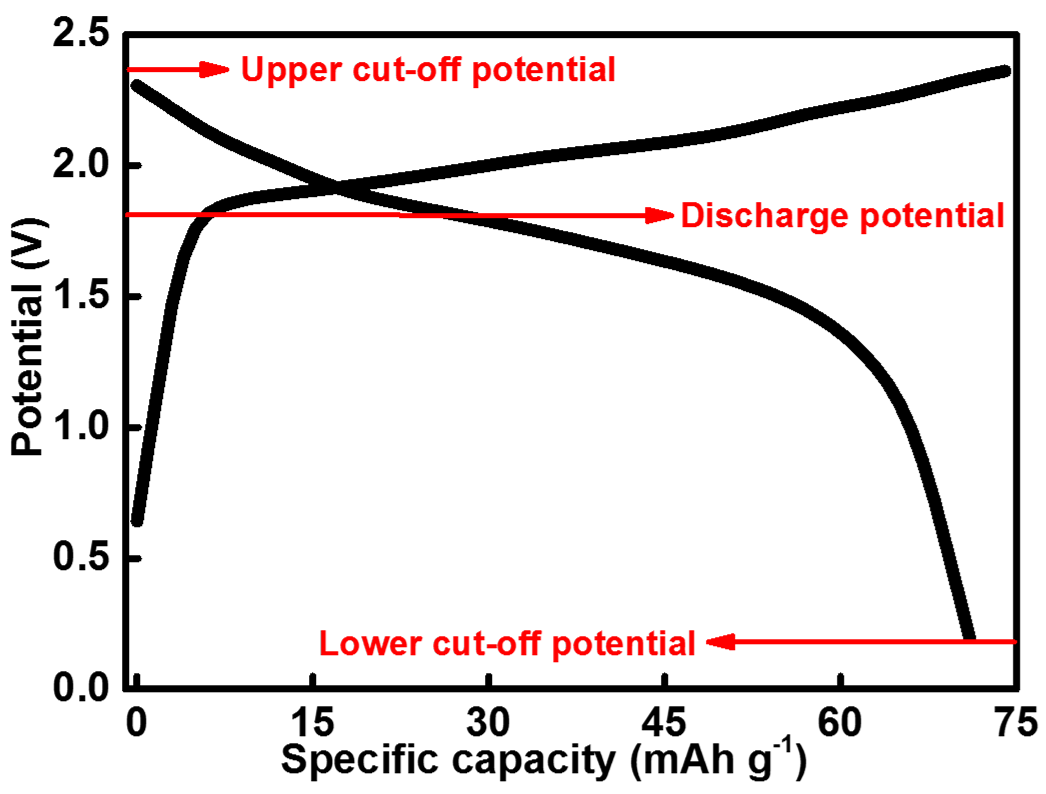
\includegraphics[width=\textwidth]{Figures/chap1fig/CDCforcellvoltage}
\caption{A charge/ discharge curve of an aluminium ion cell using graphite as the cathode and pure aluminium as the anode. The cell was charged and discharged to 2.45 V and 0.2 V respectively.}
\label{Figures/chap1fig:CDCforcellvoltage}
\end{figure}
    %While the reduction of battery voltage with discharge is a negative aspect of batteries which reduces their efficiency, one practical aspect of such a reduction, if it is approximately linear, is that at a given temperature, the battery may be used to approximate the state of charge of the battery. In systems where the battery voltage is not linear over some range of state of charge of the battery or in which there are rapid variations in the voltage with the BSOC will be more difficult to determine the BSOC and therefore will be more difficult to charge. However, a battery system that maintains a more constant voltage with discharge rate will have a high voltage efficiency and will be more easily used to drive voltage sensitive loads. Battery voltage will increase with the temperature of the system, and can be calculated by the Nernst Equation for the equilibrium battery voltage.
    
\item \textbf{Energy density}: The primary function of a battery is to store electrical energy. It is an important characteristic of a battery for any portable application, whether it’s for a laptop or an electric vehicle. Heavy batteries required to move something as large as a car over long distances need high energy density batteries. We need battery chemistries which have higher theoretical energy densities than Li-ion batteries, the current state-of-the-art. A simple way to determine the specific energy or energy density of a battery is using Eq.\ref{eq2} multiply the capacity by the battery voltage:
\begin{equation} \label{eq2}
    \text{Energy Capacity}= \text{Ah} \times \text{Battery voltage}
\end{equation}
\item \textbf{Power density}: Power density measures how quickly a battery can deliver energy. Also known as specific power, it's equivalent to the maximum current one can draw from a battery. Units used to describe power density are W kg$^{-1}$ or W m$^{-3}$. The best way to differentiate between energy and power density of a battery is to use an example of a moving car. Energy density determines how 'far' the car will go, whereas power density determines how 'fast' the car will go.
\item {\textbf{Primary and secondary batteries}}: Primary or non-rechargeable batteries produce current immediately when assembled. They have very high energy densities since it is a single-use system. Implanted medical devices, guided missiles, mars rovers and military ordnance use primary batteries. They have a low initial cost, however disposing a primary cell is problematic since the chemical reactions are not easily reversible and active materials may not return to their original states. They prove to be an uneconomical energy source since they produce only about 2\% of the power used during their production. Common types of disposable batteries include zinc–carbon and alkaline batteries. 
\textit{Secondary}, or rechargeable batteries, need to be charged before their first use. Applying an electric current (during charge) reverses the cell's active materials chemical state since they are  assembled in the discharged state. Since they can store energy reversibly, they are extensively used as energy storage devices. The oldest form of rechargeable battery is the lead–acid battery, which has been used since the 1700's. These batteries find extensive use in automotive, power tools, laptop computers, mobile phones, toys, etc. The most commonly used examples of rechargeable batteries are lithium-ion batteries, nickel-cadmium (NiCad) and nickel metal hydride (NiMH) batteries. 
\item \textbf{Coulombic efficiency}: Coulombic efficiency of a battery is the ratio of number of charges that enter during charge to the number that can be extracted from the battery during discharge.  Any loss in coulombic efficiency can be attributed to some secondary reaction (side reactions) in the battery system. A high coulombic efficiency in excess of 95\% is considered a standard value for commercial battery systems.
  
    \end{itemize}
The charging/discharging rates affect the rated battery capacity. If the battery is being discharged very quickly (i.e., the discharge current is high), then the amount of energy that can be extracted from the battery is reduced and the battery capacity is lower. This is due to the fact the necessary components for the reaction to occur do not necessarily have enough time to either move to their necessary positions. The only a fraction of the total reactants are converted to other forms, and therefore the energy available is reduced. Alternately, is the battery is discharged at a very slow rate using a low current, more energy can be extracted from the battery and the battery capacity is higher. Therefore, the battery of capacity should include the charging/discharging rate. A common way of specifying battery capacity is to provide the battery capacity as a function of the time in which it takes to fully discharge the battery (note that in practice the battery often cannot be fully discharged). The notation to specify battery capacity in this way is written as C$_x$, where x is the time in hours that it takes to discharge the battery. In the above table, C$_{10}$ (also written as C$_{10}$ = xxx) means that the battery capacity is xxx when the battery is discharged in 10 hours.The temperature of a battery will also affect the energy that can be extracted from it. At higher temperatures, the battery capacity is typically higher than at lower temperatures. However, intentionally elevating battery temperature is not an effective method to increase battery capacity as this also decreases battery lifetime. 
An ideal battery should be low-cost, get charged and discharged indefinitely under high or low current rate, have a long lifetime with high coulombic efficiency (>95\%), high energy density, and low-self discharge. However, it is very difficult to achieve the above set of requirements. Researchers are working towards various chemistries to achieve the above set of requirements. The lithium-ion battery system is a power pack of choice not only on the Earth, but also in space. It receives the most attention and is gradually replacing the nickel-based predecessors that dominated the battery world until the 1990s. Last year in October, a few astronauts on board the International Space Station (ISS) finally stepped outside their quarters for a spacewalk. Flight engineers Christina Koch and Jessica Meir (first all female spacewalk) were assigned the task of manually swapping out two nickel hydrogen (NiH) batteries for one brand new lithium-ion battery (LIB). This would not only upgrade the station's complex electrical system but also extend it's life through 2020's. ISS was launched into orbit in 1998 with 48 NiH batteries. The National Aeronautics and Space Administration (NASA) has started swapping these old batteries, since 2017, with 24 new LIBs  that provide higher energy density and a better power efficiency. Naturally, they had to be careful while handling these heavy batteries (195 kg) because they cannot be damaged or dented. LIBs come with a potential risk of \textit{thermal runaway}- defects or manhandling a battery to overheat and explode. Inside a pressurised oxygen-rich capsule, the results would have been catastrophic! NASA has found a solution for this safety concern by making batteries equipped with materials that would contain any form of leakage and prevent if from emitting heat , smoke or fire in case of combustion. 
A battery expert said that the switch from lead acid to Li-ion will be faster than the advancement of the Internet. Applied to a battery, Moore’s Law would shrink a starter battery in a car to the size of a coin.
\section{Rechargeable batteries and other power sources}
\subsection{Lead-acid batteries}
Lead acid batteries are the most commonly used type of battery in photovoltaic systems. Although lead acid batteries have a low energy density, only moderate efficiency and high maintenance requirements, they also have a long lifetime and low costs compared to other battery types. One of the singular advantages of lead acid batteries is that they are the most commonly used form of battery for most rechargeable battery applications (for example, in starting car engines), and therefore have a well-established established, mature technology base.
\subsection{Nickel-cadmium (NiCad)}
Nickel-cadmium may be cost effective on a life-cycle/cost basis. They consist of a positive electrode of nickel (or hydroxide) and a negative electrode of cadmium hydroxide. They are commonly used in a sealed configuration in small household appliances. NiCad batteries have several advantages such as a long lifetime and long storage life. The redox processes occur on the surface of the electrodes which means there is no loss of the active material. These processes increase the cell's lifetime. Furthermore, the electrolyte in nickel-cadmium is less corrosive to battery parts than in a lead-acid battery which also increases lifetime. A NiCad cell can be fully discharged and charged without damaging the battery. NiCad batteries are less sensitive to colder temperature, tolerating temperatures of -50$^{\circ}$C. In addition, the NiCad batteries have low maintenance requirements. Unlike, lead-acid batteries, NiCad batteries do not use corrosive elements and require less frequent maintenance. However, they also have a number of disadvantages. Some of the disadvantages include; Expense. Nickel-cadmium batteries are typically at least twice as expensive than lead-acid batteries and record lower coulombic efficiencies between 75\% to 85\%.

\subsection{Vanadium redox-flow batteries)}
 Redox flow batteries use a reduction-oxidation between two valence states in solution rather than changing the composition, and hence the valence states of solid material on an electrode. A flow battery consists of two volumes of solution separated by a selective membrane which allows some ions to pass but not others. Flow batteries have several potential advantages over solid batteries. A key advantage, which is particularly important in transport applications, is that the battery may be re-charged simply by pumping out the uncharged solution and replacing the solution with charged solution. This eliminates potentially long recharging times, such as are encountered in electric vehicles. Replacement of the solution allows the electric car to be recharged in the same fashion in which a car is filled with fuel. Another advantage is that the capacity of the battery is determined by the volume of solution, while the power of the battery is determined by the membrane contact area between the two solutions. The vanadium-Vanadium redox flow battery, developed at the University of New South Wales, is a particularly promising flow battery. It consists of two states of Vanadium. It has high efficiencies, with coulombic efficiencies of 97\% and energy efficiencies of 87\%. In addition, since both solutions (anode and cathode) in the battery use vanadium, cross contamination between the two solutions may discharge the battery, but will not cause damage to the battery.
\subsection{Lithium and lithium-ion (LIB)}
An electrochemical potential is a measure of the energy of the outer most electrons. Examination of the electronic configuration of the outer shell of the material gives an indication of the magnitude and sign of the electrochemical potential between the reactants and products of a redox reaction taking place inside a battery. The standard potential of a redox reaction is used to determine if a redox reaction will occur spontaneously (if it will generate a voltage between the reduction and oxidation reaction). If the difference between the standard potentials is positive, then the reaction will proceed spontaneously. If the standard potential is negative, a voltage needs to be applied in order for the reaction to proceed, which is precisely what is needed in a battery. Therefore, standard potential is an important parameter to find a suitable battery anode. Lithium has the highest electrochemical potential. It can achieve very high energy and power densities in high power battery applications. Many variations (such as lithium-ion) of the basic lithium chemistry have been developed for specific applications. Lithium is a highly flammable metal. Early commercial cells with metallic lithium cathodes were considered unsafe because of this property. However, modern cells use compounds of lithium that do not react as aggressively. A typical Li-ion cell use graphite for its anode and lithium-cobalt dioxide (LiCoO$_2$) or a lithium-manganese compound (\ce{LiMnO4}, \ce{Li2MnO3}) as cathodes. An electrolyte is a medium that allows ion-transfer inside the cell. The most commonly used electrolyte for LIBs is based on \ce{LiPF6} and mixtures of cyclic and linear carbonate solvents. The linear carbonates, such as dimethyl carbonate (DMC), ethyl methyl carbonate (EMC), or diethyl carbonate (DEC), maintain low viscosity of the electrolyte and enhance its conductivity. However, they are flammable and show flash points around room temperature (between 16 and 33$^{\circ}$C). In combination with an oxidant and an ignition source, they may catch fire and cause explosions. Using non-flammable electrolyte solvents or of flame-retardant electrolyte additives enhances the safety of flammable electrolytes, it deteriorates the electrochemical performance of batteries. 
However, LIBs have become the leading pioneers in battery technology especially for portable consumer electronics. Additionally, volume production has brought the prices down.
Mechanisms: 1. Intercalation/ deintercalation, 2. alloying/ dealloying 
\section{Aluminium-ion battery}
To find a suitable battery system, one needs to examine theoretical specific capacities of different ions that can replace lithium, using \ref{eq1}. Metals in the upper left corner of the periodic table, such as sodium (Na), magnesium (Mg), potassium (K) and calcium (Ca) reported higher theoretical capacities than the others and can be alternatively used as battery anodes. Table  \ref{table1} shows calculations for a few common metal anodes. 
\begin{table}[tbh!]
\caption{Comparing important parameters of various metal anodes.} \label{table1}
\begin{tabular}{lccccrr}
\headrow
\hline
 & \textbf{Li} & \textbf{Na} & \textbf{Mg} & \textbf{Al} & \textbf{K} & \textbf{Ca}\\
\hline
Valence electrons & 1 & 1 & 2 & 3 & 1 & 2\\
Specific capacity (mAh g$^{-1}$) & 3862 & 1166 & 2205 & 2980 & 685 & 1340\\
Standard potential (V) & -3.04 & -2.71 & -2.36  & -1.68 & -2.93 & -2.87\\
Abundance (ppm) & 18 & 22700 & 23000 & 82000 & 18400 & 41000\\
\hline  % Please only put a hline at the end of the table
\end{tabular}
\end{table}

Table \ref{table1} shows lithium to be one of the most promising candidates. An important drawback with lithium is that it is rare. Lithium and cobalt have been exhaustively used in the LIB industry and we might run out of these resources after 25-30 years. The second most promising metal is aluminium (Al), which has a relatively high standard oxidation potential. Aluminium-ion batteries (AIBs) using aluminium metal as anode will be cost-effective, easily recyclable, and much safer to use than LIBs.  In Na-ion and LIBs, a monovalent ion is intercalated/ deintercalated into/from the electrode compared to a trivalent ion in AIBs. Since three charges are involved in the redox reactions, a higher specific capacity and energy density might be obtained. The electrolyte is a chemical medium that allows the flow of charge between the cathode and anode. It acts like a catalyst by promoting the movement of ions from the cathode to the anode. The electrolyte of a battery is usually made of soluble salts, acids or other bases in liquid, gelled or dry media; it might be a polymer (in LIBs), soil or concrete (Zn-ion batteries), or ionic liquids, also known as molten salts (in AIBs). The electrolyte is there to put the different chemicals of the anode and cathode into contact with one another, in a way that the chemical potential can equilibrate from one terminal to the other, converting stored chemical energy into useful electrical energy. The ions transport current through the electrolyte while the electrons flow in the external circuit generating an electric current. 

\subsection{Aqueous aluminium-ion batteries}
Using water instead of organic solvents (flammable electrolyte in LIBs) or ionic liquids as an electrolyte would reduce the battery costs significantly and increase battery safety.
However, these batteries come with their own set of problems. 
\begin{itemize}
    \item the electrochemical plating/stripping of aluminium occurs at a
    voltage far from the stable potential window of water
    \item \ce{AlCl3}, which is used in the electrolyte, is highly acidic and sometimes results in dissolution of active material and corrosion of battery parts
    \item No cathode material has yet been reported with a good cycling stability 
\end{itemize}  
  Anatase \ce{TiO2} has been investigated as potential intercalation electrodes in aqueous AIBs. Cyclic voltammetry (CV) scans suggest an insertion redox mechanism [12]. Titanium oxide nanostructures have been commonly used as cathode materials in aqueous AIBs. Different nanostructures such as nanoleaves \cite{}, nanospheres\cite{} and nanotubes\cite{} have been tested with varying results. Using black \ce{Ti)2} nanoleaves, He et al. achieved a capacity of 271 mAh g$^{-1}$ at a current rate of 50 mA g$^{-1}$ , while TiO2 nanospheres produced a capacity of 180 mAh g$^{-1}$ at a lower current rate of 50.25 mA g$_1$ but for 30 cycles. However, given the domination of Li-ion chemistries for high energy density (specific energy) applications, more important metrics for aqueous ion cells are cycle life, efficiency and rate capability. Improving these characteristics would allow them to be competitive for a number high power applications such as regenerative braking or high power grid services [13]. Despite this, only limited focus has been given to cycle life, efficiency and rate capability in the recent aqueous Al-ion literature. Only 30 cycles are presented by He et al. and Kazazi et al. for their black TiO2 nanoleaves and TiO2 nanospheres respectively (although He et al. show 300 cycles from black nanoleaves in their supplementary material)\cite{kazazi_high_2017}. Cycling data for TiO2 nanotubes were presented up to cycle 13 by Liu et al \cite{liu_aluminum_2012}.  Recently, a graphene enhanced \ce{TiO2} electrode was shown to produce a capacity between 10 and 25 mAh g$_1$ at a current density of 6.25 A g$_1$. However, only 125 cycles were possible and coulombic efficiency was observed to be very low at approximately 50\% (estimated from figures). Similarly, the charge discharge profiles observed for the nanospheres and nanotubes show low coulombic efficiencies of around 80e85\%. The reason for the low efficiency of \ce{TiO2} in aqueous Al 3þ electrolyte has yet to be explicitly mentioned but are suggested here to be due to possible:
Oxidation of Ti3þ due to dissolved O2 in electrolyte
H2 evolution
Irreversible reduction of Ti4þ to Ti2þ during charge phases 
This paper therefore focusses on high rate capability and extended cycle life as the primary metrics of importance for aqueous Al-ion electrodes.
Rechargeable Al batteries emerge as a competitive alternative for post-lithium batteries5. As typical multi-electron reaction devices, the Al-ion batteries possess the potential of higher specific capacity, superior volumetric energy density, and comparable gravimetric energy density to lithium-ion batteries6,8,9. Moreover, the high abundancy and easy accessibility of Al resources enable Al-ion batteries to become an ideal candidate for large-scale energy storage system9. Because the standard electrode potential of Al$^{3+}$/Al (−1.68 V) is lower than \ce{H+}/\ce{H2}, the evolution of H2 occurs due to the reaction between aluminum foil and aqueous acid or alkali solution. Thus, Al cannot be electrochemically striped or deposited
in a common aqueous solution. To be compatible with Al anode, the ionic liquid \ce{AlCl3}/[EMIM]Cl with a wider range of electrochemical active window emerges as the typical electrolyte, which provides a mild corrosive effect on the Al surface to activate the Al striping and plating reaction. However, such type of ionic liquid electrolytes are not preferable for the application in large-scale energy storage systems due to its high cost and potential environmental concerns. Therefore, an alternative nonflammable and low-toxicity aqueous electrolytes for low-cost rechargeable aluminum-ion battery is urgently needed. Another critical issue that limits the application of Al batteries is the low energy density due to the lack of proper cathode materials. Thus far, there are two categories of cathode materials for rechargeable Al batteries. One is the carbon-based materials with high specific surface area such as 3D graphite-foam that can accommodate AlxCly − 12–18. Owing to the ultrafast monovalent reaction kinetics18, the 3D graphite-foam delivers a high power density of 3000Wkg−1 12. At the same time, the monovalent reaction inherently limits the obtainable specific capacity. Among the carbon-based materials, the highest reported specific capacity (graphene nanoribbons on highly porous 3D-graphene foam) was only 148 mAh g$^{−1}$ 13, which is far from practical requirements. The other category of cathode materials can realize trivalent reaction and thus have the potential to achieve high specific capacity, but they suffer from relatively lower redox potentials. It is well known that the strong electrostatic nature of Al3+ always leads to sluggish kinetics, high over-potentials, and the eventual collapse of host structure. Therefore, to accommodate trivalent \ce{Al^{3+}}, it is essential for the cathode materials to possess weak bond strengths between the host frameworks (namely, moderate polarity). The representatives with moderate polarity are sulfur, transition metal sulfides, Prussian blue analogues, and some transition metal oxide. These materials have promoted a relatively reversible trivalent reaction, but with discharge voltages only ranging from 0.3 to 0.8 V can hardly be considered as valid cathode materials. As such, there is an urgent need for the development of cathode materials for Al
batteries with high capacity and high redox potential.

\subsection{Non-aqueous aluminium-ion batteries}

\subsection{Cathodes in aluminium-ion batteries}
\section{Future outlook} 
%% Chapter 3

\chapter{Experimental methods} % Main chapter title
In this chapter we discuss the methods used when assembling a lab-scale battery for preliminary electrochemical tests. 
\label{chap3} % For referencing the chapter elsewhere, use \ref{Chapter1} 
%----------------------------------------------------------------------------------------

% Define some commands to keep the formatting separated from the content 
%----------------------------------------------------------------------------------------
\section{Components of a cathode}
A cathode consists of an active material, a binder and conductive carbon. They are mixed together to form a slurry, which is then coated on a current collector.  
\begin{itemize}
    \item Active material: The main material that gives a battery its capacity
    \item Binder: A binder is usually a polymer that uniformly binds the cathode materials and allows it to stick firmly on the current collector. Polytetrafluoroethylene (PTFE or Teflon) and Polyvinylidene fluoride (PVDF) are most commonly used as binders while making battery slurries.
    \item Conductive carbon: A conductive form of carbon which is amorphous in nature, is added to improve the conductivity of the slurry. Super-P\textsuperscript{\textregistered} or carbon black is normally used as a conductive agent. 
    \item Current collector: Typically a metallic foil (copper, aluminium, steel, etc.) connected to the electrode with external loading. The main role of the current collector is to support the electrode and to collect the accumulated electrical energy from the electrode\cite{sun_effect_2017}.
\end{itemize}
\section{Formation of slurry}
A slurry is a paste-like substance used in making battery electrodes. It is important for slurries to be homogeneous. This helps in getting a uniform coating at later stages.  PVDF was mixed separately in an organic solvent, N-methyl pyrrolidinone (NMP). This viscous solution was added to the mixture of active material and Super-P\textsuperscript{\textregistered} . NMP can be added later to adjust the consistency of the slurry. It was then mixed on a magnetic stirrer for 8-10 hours. 
\section{Preparing a cathode}
Once the slurry was prepared, it was 'doctor-bladed' on a current collector. Doctor blading is a coating process where the slurry spreads on a substrate (molybdenum foil)  using a blade, to form a this sheet which dries off to give a layer of coating.  Initially, we used nickel foils as current collectors, however we found that Ni oxidised at $\sim$ 1.0 V. This did not allow the cell to reach it's cut-off potential at 2.4 V. It impeded the cell's redox processes, which reduced the cell's capacity. After trying a few current collectors, we found that molybdenum foil was inert in this cell chemistry (discussed in Appendix A) and was used in all our battery systems. After coating the foils with the slurry, the electrodes were dried at 80$^{\circ}$ C for two hours to improve the adhesion of the slurry onto molybdenum foil. 
\begin{figure}[tbh!]
\centering
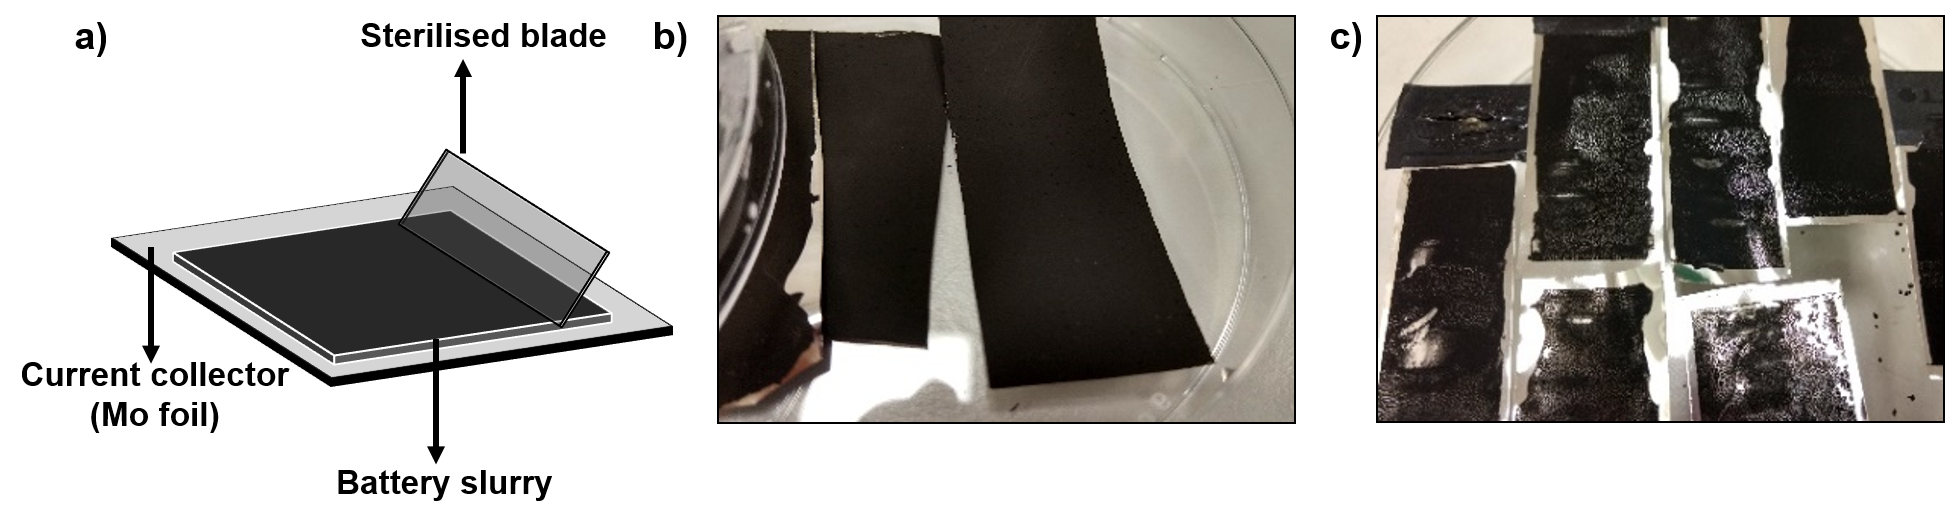
\includegraphics[width=\textwidth]{Figures/chap3fig/coating}
\caption{a) Doctor-blading on a current foil using a steel blade. A dried cathode after b) uniform and c) non-uniform coating.}
\label{Figures/chap3fig:coating}
\end{figure}
\section{Vacuum drying}
Vacuum drying is a moisture-removal technique by means of creating a vacuum. Vacuum drying is used for drying things which are hygroscopic (water sensitive). IA vacuum is created to decrease the chamber pressure below vapor pressure of the solvent (NMP), causing it to boil. This increases its rate of evaporation and increases the drying rate of the product. The pressure maintained in vacuum drying is generally 0.03–0.06 atm. The cathodes are ready for use after drying. 
\section{Assembling a cell}
Using pouch cells or coin cells (CR-2032\textregistered) is a common practice amongst researchers working on batteries. CR-2032 is made of steel and could not be used in our experiments. Since our electrolyte reacts with steel, we switched to custom-made cells that used PEEK (polyether ether ketone) for the main body and steel rods as plungers that would push the electrodes towards each other. PEEK  is a colourless organic thermoplastic polymer. It has a melting point of 343$^{\circ}$C, with excellent mechanical and chemical resistance properties. Steel rods were later replaced with molybdenum rods because of above mentioned reasons. 
\begin{figure}[tbh!]
\centering
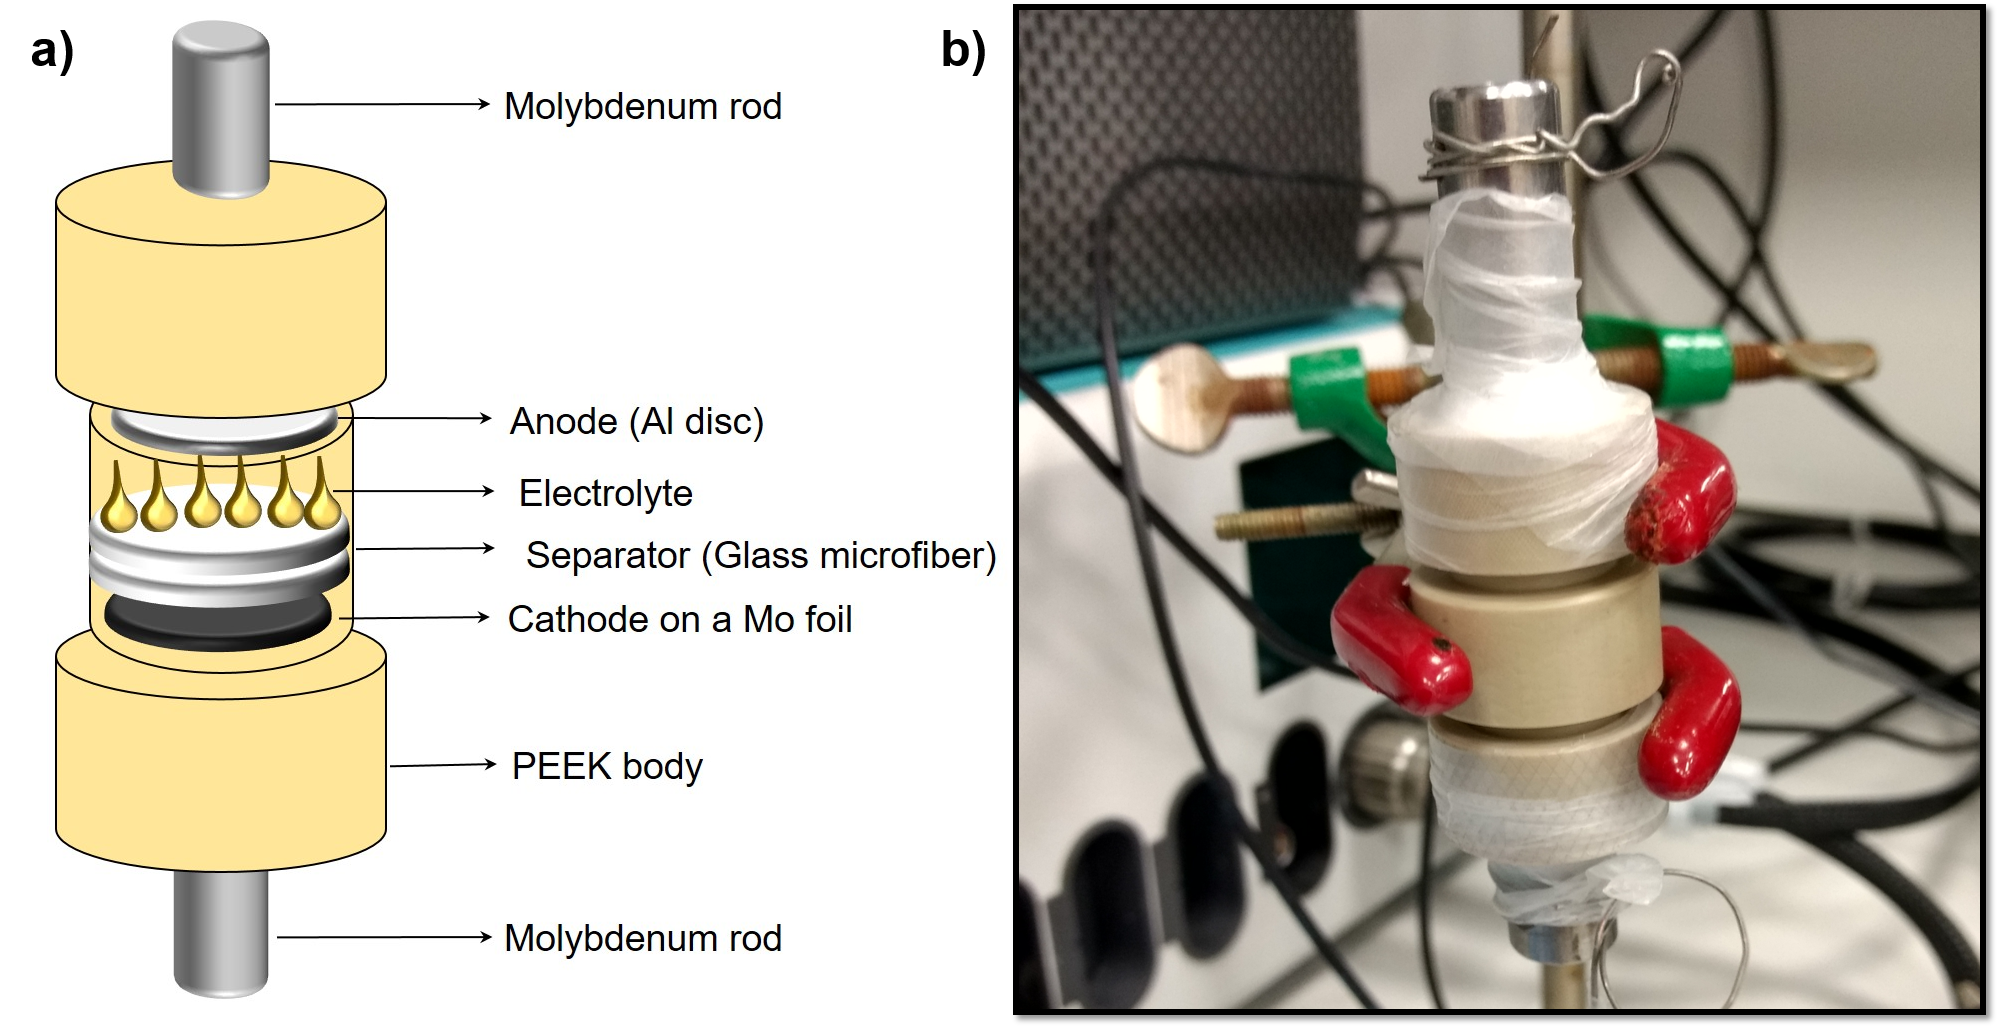
\includegraphics[width=\textwidth]{Figures/chap3fig/swagelok}
\caption{a) Assembling a two-electrode PEEK cell using a cathode, separators wetted with electrolyte and an anode. Mo rods were used as plungers and Mo sheets was used as current collector. b) A custom-made lab cell ready for preliminary electrochemical measurements.}
\label{Figures/chap3fig:swagelok}
\end{figure}
A cathode was placed at the bottom of the cell, two separators made of glass microfibers were put above the cathode. Electrolyte was then added ($\sim$80 $\mu$l) until the separators were completely wet. An anode which was 99\% pure aluminium foil was cut into a disc and placed on top and the cell was then screwed tight, shown in Figure \ref{Figures/chap3fig:swagelok}a. Since the electrolyte is hygroscopic, the cell was assembled inside a glove box with <0.1ppm \ce{O2},\ce{H2O}. The cell was taken out of the glove box and wrapped tightly with a paraffin film to further inhibit contact with moisture or air, as shown in Figure \ref{Figures/chap3fig:swagelok}b. The cells were ready for electrochemical measurements . 





















 
%% Chapter 1
\section*{\centering Preface}
This chapter discusses the characterisation techniques that were implemented post-mortem, to fully analyse how a battery works. Electrochemical processes such as cyclic voltammetry and galvanostatic charge/ discharge curves have been discussed in detail.   

\pagebreak

\chapter{Techniques for characterisation} % Main chapter title

\label{chap2} % For referencing the chapter elsewhere, use \ref{Chapter1} 

Performance of a battery cannot be assessed without galvanostatic charge and discharge cycles and cyclic voltammetry (CV). Battery potential is determined by the stability of its electrolyte. CV scans help in determining the voltage range of a cell. A charge/discharge cycle (CDC) on the other hand helps in evaluating a cell's specific capacity and nominal (discharge) voltage. Long term CDCs are necessary to verify a cell's stability and observe whether it can be put to commercial use or not. 
During continuous charge and discharge, a cathode material undergoes many changes. For example, distance between two layers should increase when intercalation takes place. Or, the oxidation states of a metal should change when it oxidises or reduces itself during cycles. Analytical tools are needed to study the following changes. 

\begin{itemize}
    \item Changes in the crystal lattice of a material can be studied in its XRD patterns 
    \item Changes in the oxidation state of an element can be noticed in its XPS spectra
    \item Changes in the vibrational mode of a molecule can be observed in its Raman spectra 
\end{itemize}

\section{Galvanostatic charge/discharge cycles}
Galvanostatic charge and discharge is a method to evaluate the amount of charge stored in a cell, typically under constant current. The technique measures voltage at a controlled or fixed current rate. Since the current is repeatedly reversed, it is also known as 'cyclic chronopotentiometry'. It is used to estimate the specific capacity and cycling stability of a cell. The total quantity of electricity per mass available from a fully charged cell can be calculated, from the charge transferred during discharge in terms of mAh g$^{-1}$. Specific discharge capacity is frequently measured at different discharging rates to establish rate capability of a cell \cite{pyun_electrochemistry_2012-1}. The voltage profile obtained can be used to identify multi-step redox reactions, in Figure \ref{Figures/chap2fig:ChrononCDC}. 

\begin{figure}[th!]
\centering
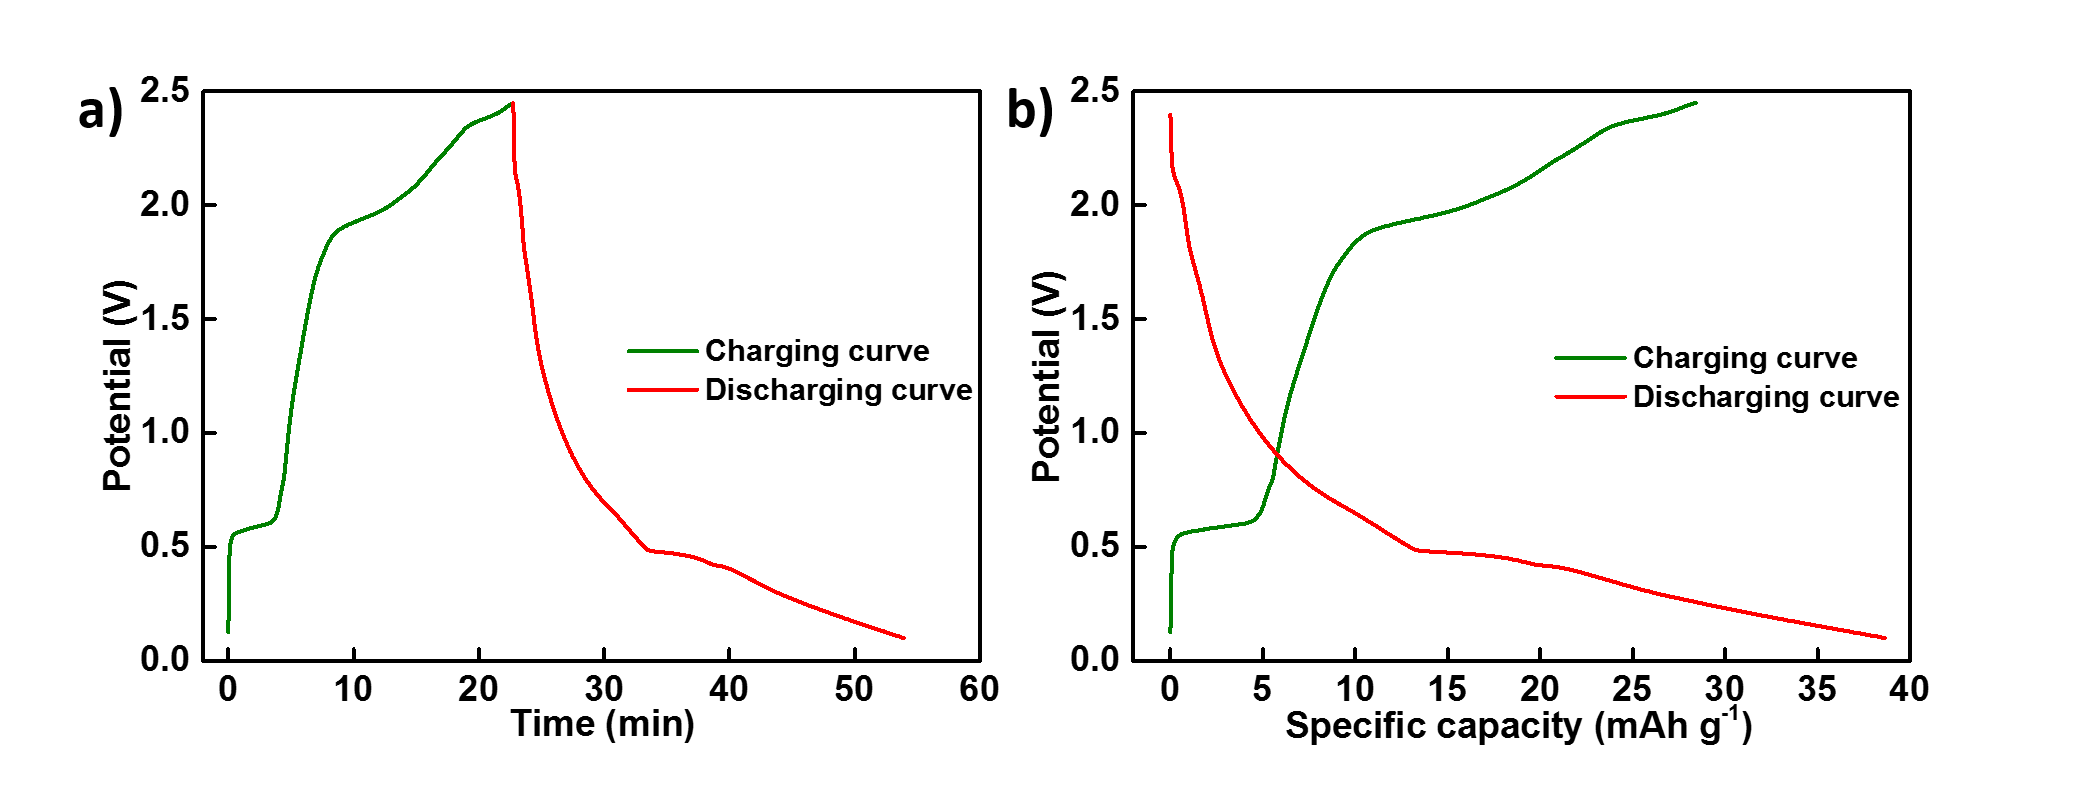
\includegraphics[width=\textwidth]{Figures/chap2fig/ChrononCDC}
\caption{a) Chronopotentiogram- a graph of electric potential versus time, at constant current. b) A galvanostatic charge/discharge curve showing the voltage plateaus at which reactions occur and the charging/discharging capacity.}
\label{Figures/chap2fig:ChrononCDC}
\end{figure}

\section{Cyclic voltammetry}
Cyclic voltammetry (CV) is a technique which measures the current that develops in an electrochemical cell during oxidation and reduction of an analyte (say M). It is performed by cycling the potential of a working electrode, and measuring the resulting current. In Figure \ref{Figures/chap2fig:CV}, we started a forward sweep with a positive scan (lower potential to higher potential). S1 is called a switch potential where the voltage is sufficient enough to cause an oxidation or reduction, and the scan is reversed. Potential is then swept negatively (higher potential to lower potential) until it reaches S2 (another switch potential). In an ideal situation, during forward sweep, M is depleted from the solution as it gets oxidised to \ce{M+}. Further oxidation after scanning higher potentials, leads to growth of a diffusion layer (solution containing M/\ce{M+} ions) at the electrode surface throughout the scan. The layer continues to expand until a certain point, recording maximum current density. However, since diffusion layer continues to grow at this stage, flux of M from the bulk solution to electrode surface decreases. Therefore, current starts to decrease and we get an oxidation peak. A reverse scan converts \ce{M+} back to M (reduction) via similar pathway- formation of a diffusion layer containing M and eventually we record a reduction peak. The two peaks are separated due to the diffusion of the analyte to and from the electrode. If the reduction process is chemically and electrochemically reversible, a peak-to-peak separation of 57 mV is observed \cite{bard_electrochemical_1980}. When there is a high barrier to electrochemical irreversibility, electron transfer reactions are sluggish and more positive/negative potentials are required to observe oxidation/reduction reactions respectively. 

\begin{figure}[tbh!]
\centering
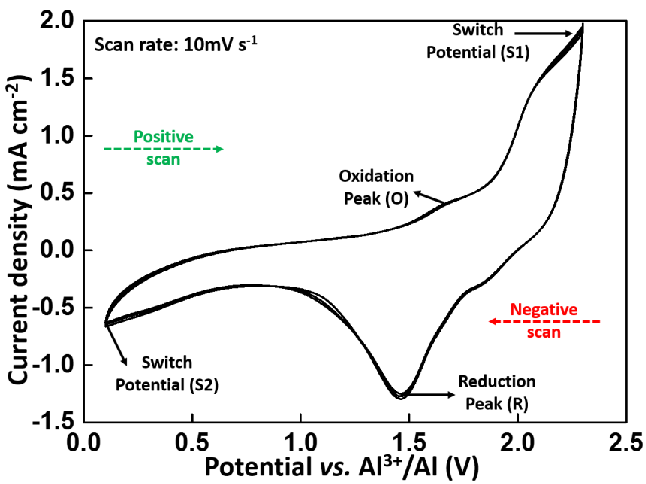
\includegraphics[width=\textwidth]{Figures/chap2fig/CV}
\caption{Cyclic voltammogram of an AIB at a scan rate of 10 mV s$^{-1}$ using a two-electrode cell with aluminium foil acting as a counter and reference electrode.}
\label{Figures/chap2fig:CV}
\end{figure}

Scan rates play a very important role too. If a CV is run on a slower scan rate (0.05 mV s$^{-1}$), diffusion layer grows farther from the electrode, which reduces the flux, consequently decreasing the current value. At a faster scan rate lead (1 V s$^{-1}$), the size of the diffusion layer decreases and higher currents are recorded. Cyclic voltammetry is a helpful tool in understanding the presence of a surface reaction and its reversibility during cell cycles. It can be used for both single-electron and multi-electron processes.  

\section*{Sample preparation}
The cell was disassembled inside a glove box to prevent the cathode from any contact with air or moisture. The cathode was taken out and washed with dry ethanol to get rid of any remaining electrolyte on its surface. It was found that scrapping off the active material from the current collector did not yield enough sample for analysis, since some of it got wasted in the process. Thus, cathode, including the current collector, was used for X-ray diffraction, Raman and X-ray photoelectron spectroscopic analyses.

\section{X-ray diffraction Studies}
Diffraction of x-rays by crystal planes allows us to derive lattice spacings by using Bragg's law. 

 \begin{equation} \label{eq2-1}
     2d\sin\theta \text= n{\lambda}
 \end{equation}
 where d = spacing between diffracting planes,\\
$\theta$ = incident angle,\\ 
n = any integer, and \\
$\lambda$ = wavelength of the incident beam. X-rays produce the diffraction pattern because their wavelength $\lambda$ is typically the same order of magnitude (1-100 $\AA$ ) as the d-spacing between the crystal planes. According to equation \ref{eq2-1} any decrease in 2$\theta$ suggests an increase in the d-spacing. 
A pure crystalline sample such as \ce{MoS2} (Figure \ref{Figures/chap2fig:XRD}a) yields sharp peaks in a XRD pattern since it has a long ordered structure. Random orientation of the powdered material is attained after scanning the sample through a range of 2$\theta$ angles. Conversion of the diffraction peaks to d-spacings allows identification of the sample because each sample has a unique set of d-spacings. Typically, d-spacings of the sample are compared with standard reference patterns (International Centre for Diffraction Data, ICDD). For determination of unit cell parameters, each reflection implies a specific lattice plane indicated by miller indices \textit{hkl} (labelled in red  for \ce{MoS2} crystal lattice). Figure \ref{Figures/chap2fig:XRD}b displays the diffraction pattern of activated carbon obtained from human hair. Since the structure of activated carbon is much less ordered, its pattern shows line broadening of the major diffraction bands, which exist at $\sim$ 25$^{\circ}$  and $\sim$ 44$^{\circ}$.
X-ray diffraction studies is a useful tool and can easily help in proving intercalation of ions. Rani \textit{et al.} used fluorinated graphite as a cathode for AIBs. The d-spacing values of the discharged graphite cathode were higher than natural graphite. The results indicate that intercalation of aluminum ions in the graphene sheets increase the d-spacing of the graphite crystal\cite{rani_fluorinated_2013-1}.
%X-ray diffraction shows line broadening of only the principal graphite diffraction bands. This broadening is usually interpreted in terms of dimensions of a hypothetical crystallite. Although the crystallite concept has been used when comparing structures in carbons, it has to be stressed that the crystallite does not exist as such within these structures. The disorganized carbon are present in cross-linkage structures [15] forming non-crystallite structures to form microstructures! 
Panalytical X-Ray diffractometer was used to record the XRD patterns using Cu-K$\alpha$ radiation at an operating voltage of 45 kV and a 40 mA current. The patterns were run with copper radiation ($\lambda$ =1.5405\AA) at a scanning speed of 2$^{\circ}$ in 20 minutes. 

\begin{figure}[tbh!]
\centering
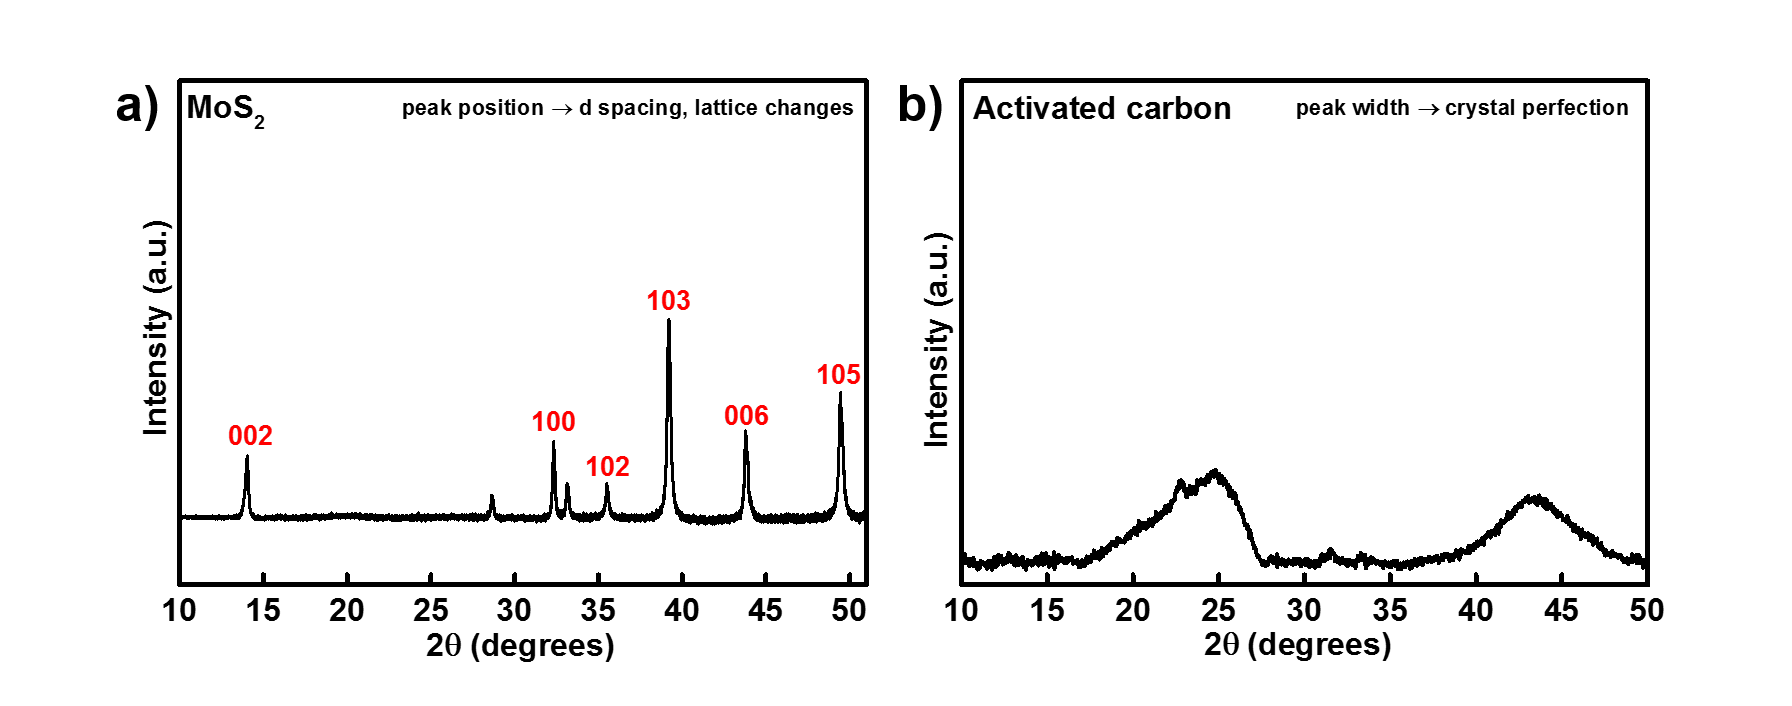
\includegraphics[width=\textwidth]{Figures/chap2fig/XRD}
\caption{X-ray diffraction pattern of a) bulk molybdenum disulfide (ICDD: 04-001-9285), and b) activated carbon.}
\label{Figures/chap2fig:XRD}
\end{figure}

\section{Raman spectroscopy}
Raman spectroscopy is a technique, which is used to determine vibrational modes of a molecule. A source of monochromatic light, usually from a laser, interacts with molecular vibrations in the system, resulting in the energy of the laser photons being shifted up (blue shift) or down (red shift). The shift in energy gives information about any changes taking place in the vibrational modes of a material. 
%This technique uses the inelastic scattering of photons, also known as Raman scattering. 
\begin{figure}[tbh!]
\centering
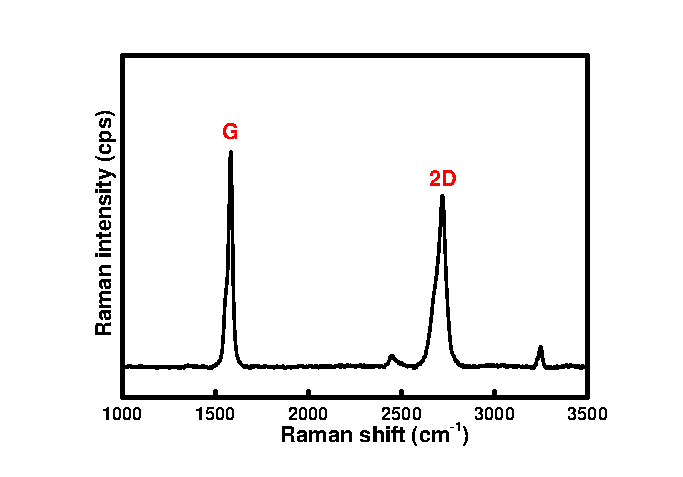
\includegraphics[width=\textwidth]{Figures/chap2fig/Raman}
\caption{Raman spectra of graphite.}
\label{Figures/chap2fig:Raman}
\end{figure}

Graphite is composed of \ce{sp2} bonded carbon atoms in planar sheets. The bond energy of the \ce{sp2} bonds displays its vibrational frequency at 1582 cm$^{-1}$. The presence of additional bands in graphite spectrum indicate that there are some carbon bonds at different bond energies. The D band indicates presence of some disorder in the structure. The ratio of intensity of D/G peaks is a measure of the defects present. Both D and G peaks are the result of vibrations of \ce{sp2} bonded carbon atoms. G band is an outcome of in-plane vibrations, whereas the D peak is due to out of plane vibrations attributed to the presence of structural defects. If the D band is more intense, it means that the \ce{sp2} bonds are broken which in turn means that there are more \ce{sp3} bonds, there will be a maximum D/G ratio. If I$_D$/I$_G$ ratio is higher than pristine sample, it means that defects are present on the material. 
Raman spectroscopy is a helpful technique in detecting the mechanism of an intercalation-based battery. Wang \textit{et al.} used Raman spectroscopy to show two different intercalation processes involving chloroaluminate anions in a graphite cathode. The Raman data pointed to two different intercalation processes at two different charging plateaus. The first plateau in the charging curve showed G band splitting and the higher voltage plateau showed a single, dominant blue-shifted peak. During discharge, the opposite trends were observed when chloroaluminate anions were deintercalated. The original graphite spectrum was recovered when the cell was fully discharged\cite{wang_advanced_2017}. 

\section{X-ray photoelectron spectroscopy}
 X-ray photoelectron spectroscopy is used to measure elemental composition and oxidation states of various elements. It is a surface-based technique that quantitatively analyses a sample. By irradiating a sample with a beam of X-rays, kinetic energy and number of electrons escaping from the top 10 nm of the sample are measured. 
%The instrument requires high vacuum (10$^{-8}$ millibar) conditions to count these electrons. The electron emission after irradiation is also called a 'photoelectron effect'. These electrons are separated according to their energies and counted. ,
A normal XPS spectrum is a plot of the number of electrons detected versus the binding energy of the electrons detected. XPS helps in studying the redox processes that take place inside a cell. XPS helps in characterising elements species and valence changes of original sample and sample during electrochemical reactions. Understanding curve-fitting of an XPS spectra is important as it suggests the number of chemical states and therefore number of peaks present in a sample. It is essential to apply constraints to restrict the peak widths and relative intensities of the peaks. The peaks were fitted using Shirley background and any observed peak was convoluted using Gaussian and Lorentzian function. \\
Li \textit{et al.} studied the XPS spectra of \ce{MoS2} microspheres to probe the valence changes and the Al$^{3+}$ storage mechanism during the charging/ discharging process at various charge and discharge states of the cathode \cite{li_rechargeable_2018-2}.

\begin{figure}[tbh!]
\centering
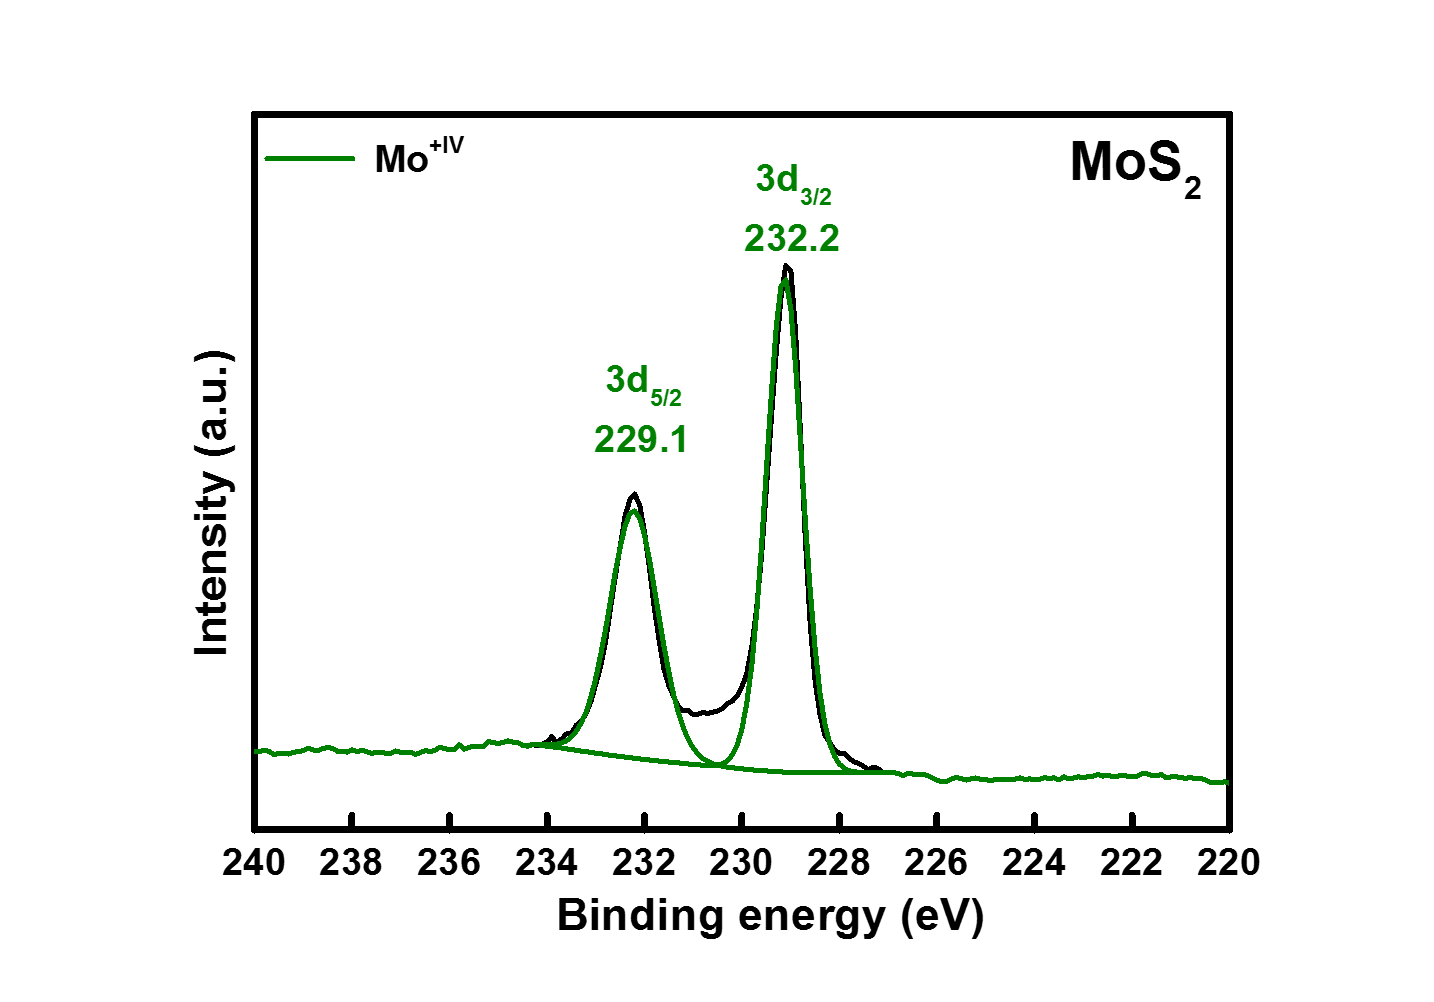
\includegraphics[width=\textwidth]{Figures/chap2fig/XPS}
\caption{X-ray photoelectron spectra of molybdenum disulfide. Molybdenum 3d orbitals appear as a doublet at 229 and 232 eV. The area ratio for the two peaks (3d$_{3/2}$ : 3d$_{5/2}$) was 2:3 (corresponding to two electrons in the 3d$_{3/2}$ level and 4 electrons in the 3d$_{5/2}$ level).}
\label{Figures/chap2fig:XPS}
\end{figure}





%\section*{Preface}
In this chapter, we discuss performance of AIBs using two-dimensional molybdenum dichalcogenides such as \ce{MoS2}, \ce{MoSe2} and MoSSe in their bulk and nano form, as cathodes for AIBs attempt to establish their mechanism. We explored different molybdenum dichalcogenide-based cathodes and their mechanism of energy storage. We expected that two-dimensional (2D) layered materials that support intercalation of charged species might be suitable as active cathode materials in AIBs. 
\pagebreak
\chapter{Molybdenum dichalcogenides as cathodes for rechargeable AIBs} % Main chapter title

\label{chap4} % For referencing the chapter elsewhere, use \ref{Chapter1} 

\section{Theory and background}
Transition metal dichalcogenides (TMDs) have a strong in-plane covalent bonding and weaker van der Waals (vdW) bonds exist between any two layers, which is quite similar to graphene layers in graphite. The 2D structure facilitates intercalation of ions within these layers. Molybdenum dichalcogenides not only provide redox variability but also a high theoretical capacity (600-1200 mAh g$^{-1}$). The intercalation voltage observed with \ce{MX2}, where M = Mo, W, Ti, etc. and X = S and Se, is high ($\approx$ 2.0 V). The mechanism that TMDs follow is based on intercalation as well as conversion. 
Molybdenum dichalcogenides (\ce{MoX2} where X=S, Se or Te) display similar properties as graphite. They have a 2D-layered structure, which allows intercalation of ions and are electrically conductive. Lower volumetric expansion on cycling is an advantage these materials have over graphitic cathodes \cite{liang_rechargeable_2011, huang_molybdenum_2019}. Amongst various transition metal chalcogenides, \ce{MoS2} has been extensively studied as a cathode for rechargeable batteries \cite{li_mos2_2004, zhu_fast_2015}, making them attractive candidates for AIB cathodes. In 2015, Geng \textit{et al.} found that \ce{Al^3+} ions fully intercalated into chevrel phase \ce{Mo6S8} with the cations occupying two different sites in the crystal lattice \cite{geng_reversible_2015}. This mechanism was called the 'rocking chair' mechanism where charge carrying species shuttled back and forth between intercalating electrodes during cycles while the overall electrolyte concentration remains constant. The discharging and charging reactions at the anode (equation 1) and cathode (equation 2) were proposed as follows:

\begin{align}
          \ce{Al + 7AlCl4^-} &\rightleftharpoons 4\ce{Al2Cl7^- + 3e^-}\\
\ce{8AlCl7^- + 6e^- + Mo6S8 &\rightleftharpoons Al2Mo6S8 + 14AlCl4^-}
\end{align}

Three years later, Li \textit{et al.} prepared \ce{MoS2} microspheres by a simple hydrothermal method \cite{li_rechargeable_2018-2}. They proposed a similar mechanism where \ce{Al^3+} ions inserted into the electrode accompanied by a phase transformation at the electrode interface. Li and his group confirmed this phase-transition by using \textit{ex-situ} XPS and XRD etching techniques. The reaction equations for this battery system at the cathode (equation 3) and anode (equation 4) were proposed as follows:
\begin{align}
    \ce{MoS2 + x\ce{Al^{3+}}  + 3x\ce{e-} &\rightleftharpoons Al_xMoS2}\\
    \ce{Al} + 7x\ce{AlCl4-} &\rightleftharpoons 4x\ce{Al2Cl7-} + 3x\ce{e-}
\end{align}

In general, these cells showed low energy density and had reversibility issues in the redox processes. It has been reported that transition metal dichalcogenide electrodes tend to transition from a 2H phase into a more conducting 1T phase when used in a battery \cite{fan_hybrid_2017}. A hybrid \ce{Mg^{2+}}/\ce{Li+} cell was tested using bulk \ce{MoS2} as a cathode material. During cyclic voltammetry (CV) scans, the authors associated the first cathodic peak, with a phase transition. 2H phase \ce{MoS2} was converted to 1T phase during initial ion intercalation. This seems to be a common phenomenon for molybdenum dichalcogenides, since Li \textit{et al.} observed similar transitions in sodium ion batteries \cite{li_enhancing_2015}. It mostly takes place during the first cycle and since the phase change is irreversible, it can be detected in a cyclic voltammogram.

This chapter documents a range of 2D molybdenum dichalcogenides including \ce{MoS2}, \ce{MoSe2} and \ce{MoSSe}, as cathodes for non-aqueous AIBs. Our unpublished, preliminary density functional theory (DFT) calculations indicated a significant decrease in inter-layer spacing of these materials when \ce{Al^3+} cations were assumed to intercalate (owing to the very high charge density of \ce{Al^3+}). Therefore, we propose intercalation of structurally distorted \ce{AlCl4-} anions into the cathode layers. Surprisingly we found that \ce{MoSe2}-based cathodes performed different and better than all of the other molybdenum dichalcogenides.

\section{Experimental methods}
Same as discussed in Chapter 3.

\section{Results and Discussion}
Figure \ref{Figures/chap4fig:S1} shows the crystal structure of \ce{MoX2} where X is sulfur (S) and/or selenium (Se). The material has two vacant sites for intercalation --- M1 and M2. M1 denotes the spaces in between the X-Mo-X atoms, whereas M2 represents the space created between the \ce{MoX2} layers as shown in Figure \ref{Figures/chap4fig:S1} a). The inter-layer distance in \ce{MoX2} is 6.3 \AA\ with a gallery height of 3 \AA. The layers are held together by weak van der Waals (vdW) forces. M2 presents an open network and provides various interstitial sites for intercalation. Since \ce{AlCl4-} ions are 5.28 \AA\ in diameter, as reported by Takahashi {\it et al.} \cite{takahashi_niv2o5nh2o_2005}, they undergo some distortion during intercalation to fit into these layers. Our preliminary results showed that \ce{Al^{3+}} would \lq contract\rq\ the \ce{MoX2} layers when trying to intercalate, making \ce{AlCl4-} anion intercalation more likely. Also, the triply charged \ce{Al^{3+}} cation has to overcome strong electrostatic forces from the \ce{S^{2-}} or \ce{Se^{2-}} anion network in order to enter, making the intercalation process slow and most likely not reversible. Therefore, we propose intercalation of \ce{AlCl4-} anions from the electrolyte into M2 sites of \ce{MoX2} during charge. Galvanostatic cycles, cyclic voltammetry (CV), X-Ray diffraction (XRD), Raman spectra and X-Ray Photoelectron Spectroscopy (XPS) results discussed later, strongly support our claim of a reversible intercalation process especially in \ce{MoSe2}.

\begin{figure}
  \centering
  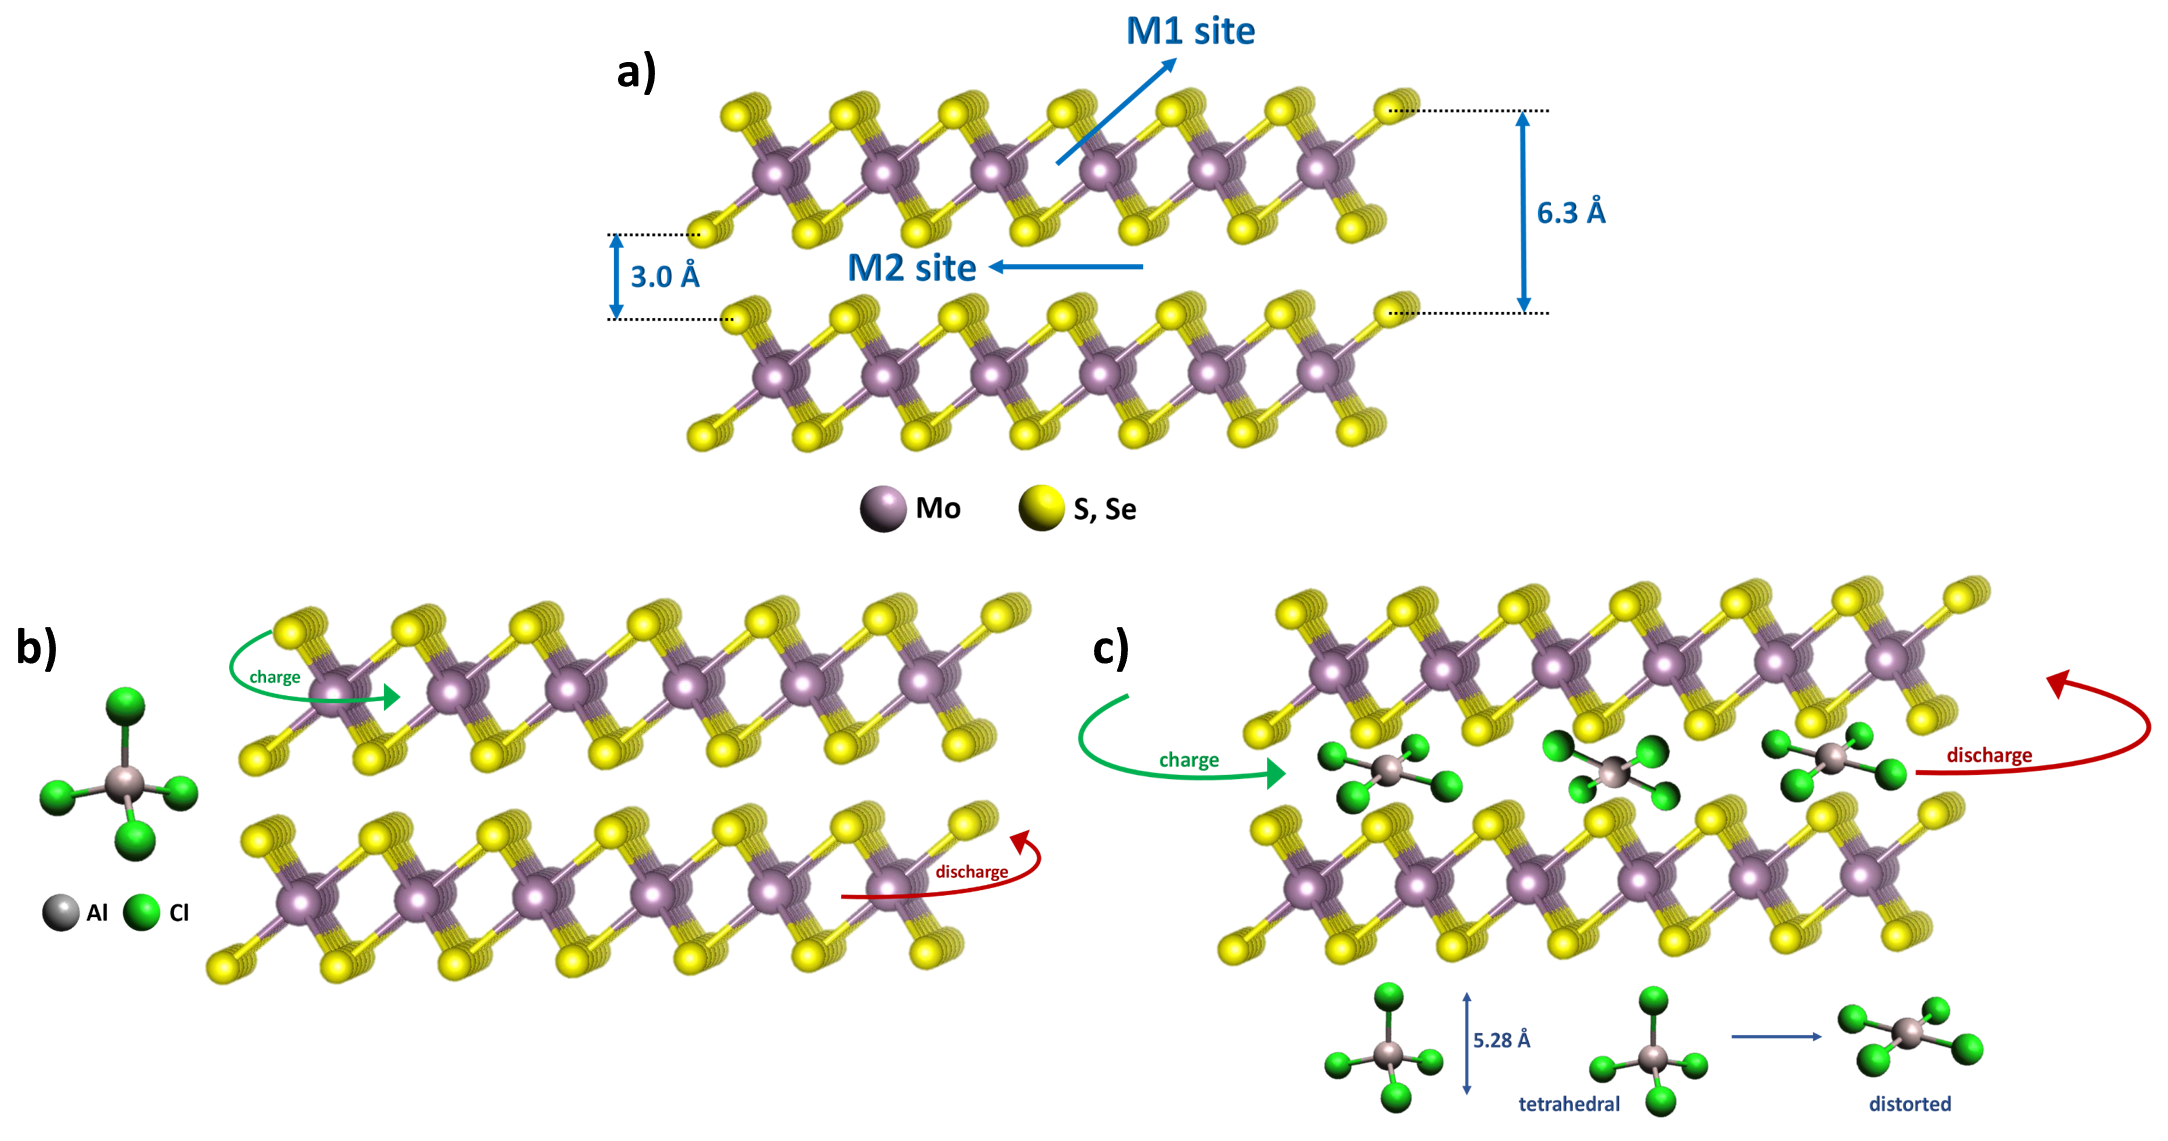
\includegraphics[width=\textwidth]{Figures/chap4fig/S1}
  \caption{Schematic representation of a) a \ce{MoX2} crystal structure with possible intercalation sites at M1 and M2 b) intercalation at M1 site and c) intercalation at M2 site.}
  \label{Figures/chap4fig:S1}
\end{figure}

\begin{figure}[htb!]
\centering
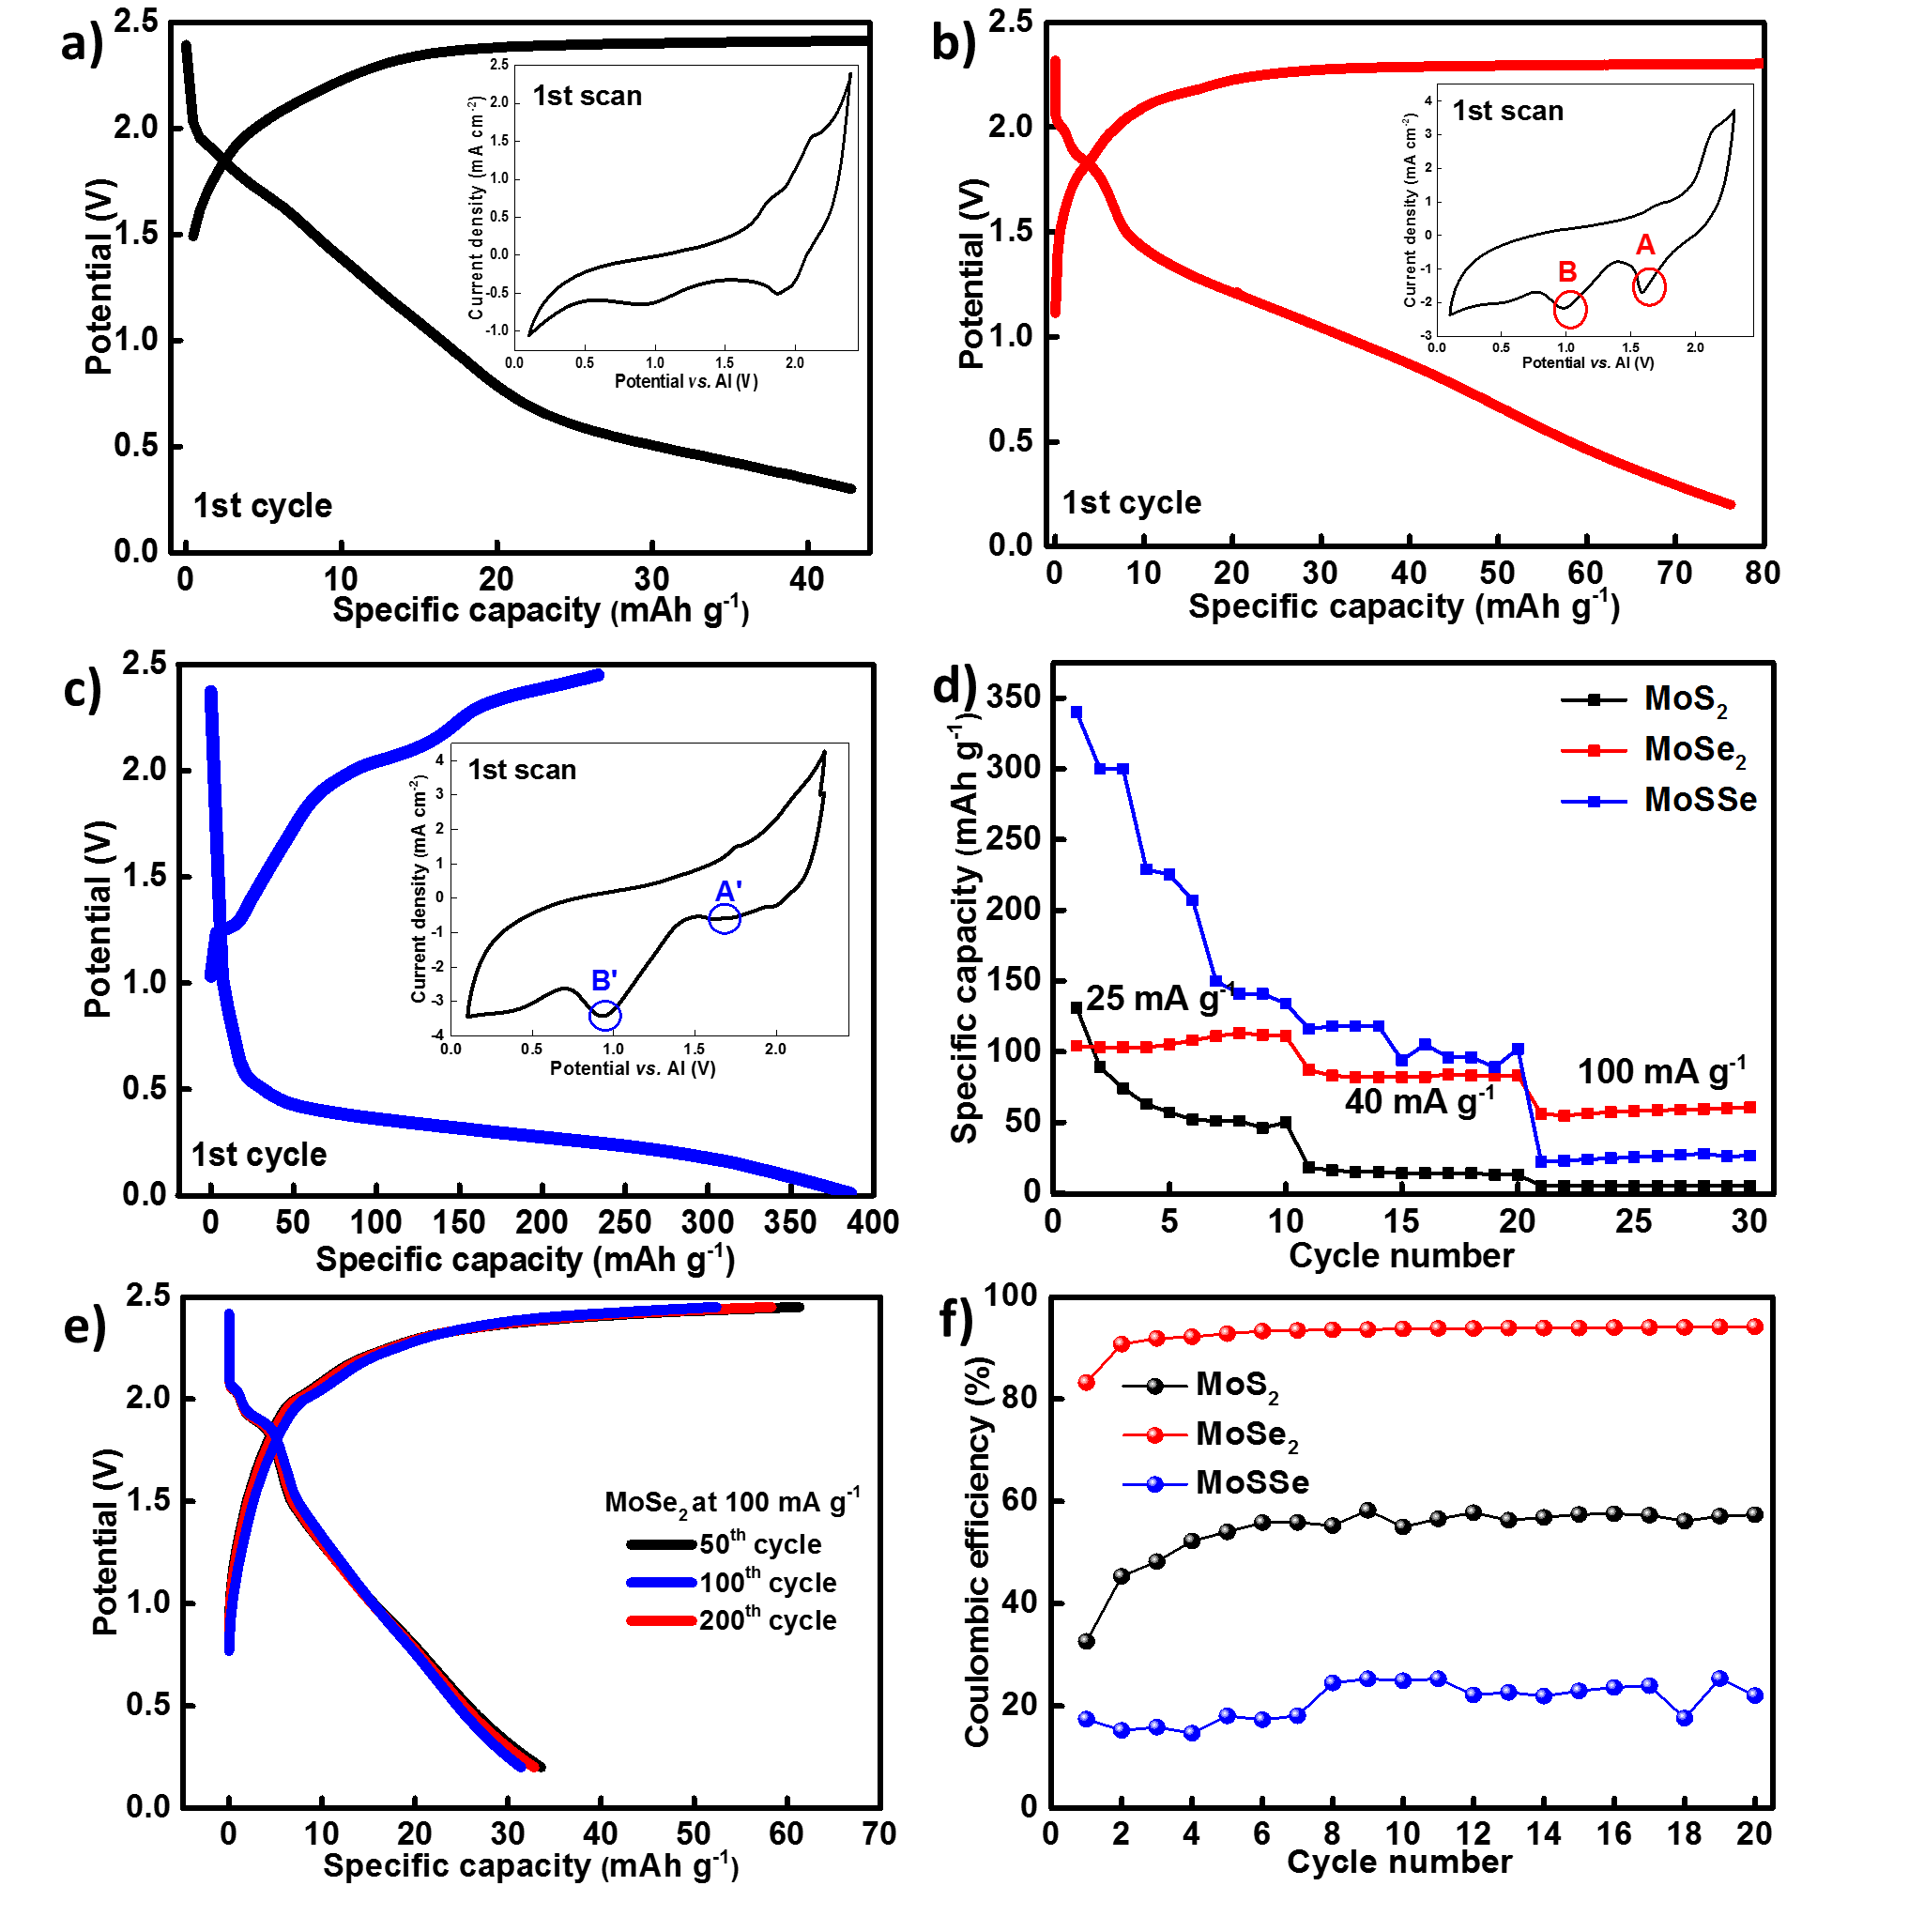
\includegraphics[width=\textwidth]{Figures/chap4fig/MoX2CDCCV}
\caption{First charge/discharge curve at 40 mA g$^{-1}$ for a) \ce{MoS2}, b) \ce{MoSe2} and c) MoSSe. d) Specific capacities of \ce{MoS2}, \ce{MoSe2} and MoSSe at current rates of 25, 40 and 100 mA g$^{-1}$. e)First CV scan of \ce{MoS2}, f) \ce{MoSe2} and g) MoSSe at a scan rate of 10 mV s$^{-1}$ in an aluminium-ion battery against Al reference electrode.}
\label{Figures/chap4fig:MoX2CDCCV}
\end{figure} 

Figure \ref{Figures/chap4fig:MoX2CDCCV} a)--c) shows the charge/discharge cycles (CDCs) for \ce{MoS2}, \ce{MoSe2} and MoSSe at a current rate of 40 mA g$^{-1}$. The discharge capacity of Al/\ce{MoS2} in its first cycle was found at $\sim$45 mAh g$^{-1}$, Figure \ref{Figures/chap4fig:MoX2CDCCV} a). Comparing this with its first CV scan (Figure \ref{Figures/chap4fig:MoX2CDCCV} g), a good correlation between the discharge voltage plateau and reduction peaks, and other redox features was found. With discharge plateaus at 1.9 V and 1.7 V, the first CV scan for \ce{MoSe2} displayed two reduction peaks at 1.65 V (point A) and 1.0 V (point B), Figures \ref{Figures/chap4fig:MoX2CDCCV} b) and \ref{Figures/chap4fig:MoX2CDCCV} h). The peak at 1.0 V suggested an irreversible reaction since this peak was absent in the following scans. Based on this, we agree with Li \textit{et al.}'s interpretation and attributed this peak to an irreversible phase transition \cite{li_enhancing_2015}. During this transition, the semi-conducting 2H phase converted into a more metallic 1T phase. This transition seemed to increase the interlayer spacing of \ce{MoSe2} by reducing the vdW forces that exist between the two layers \cite{fan_hybrid_2017}. Al/MoSSe cells showed three distinct plateaus during charging at 1.2 V, 2.0 V and 2.3 V in its first cycle, with a discharge plateau at 0.5 V shown in Figure \ref{Figures/chap4fig:MoX2CDCCV} c). Capacities of all molybdenum dichalcogenides were recorded at different current rates of 25, 40 and 100 mA g$^{-1}$, and displayed in Figure \ref{Figures/chap4fig:MoX2CDCCV} d). Since \ce{MoSe2} displayed stable specific capacities at all current rates, we recorded further 200 cycles at the highest current rate of 100 mA g$^{-1}$. A highly reversible electrochemical reaction was observed since the capacity remained at 30-32 mAh g$^{-1}$ after 200 cycles (Figure \ref{Figures/chap4fig:MoX2CDCCV} e)). The presence of multiple charging plateaus in MoSSe might correspond to various oxidation processes occurring when \ce{AlCl4-} interacts individually with S and Se atoms. The first CV scan in Figure \ref{Figures/chap4fig:MoX2CDCCV} i) showed an irreversible reduction potential at 0.9 V, point B', like \ce{MoSe2}, implying a similar phase transition. It seems MoSSe undergoes a lattice distortion and the material loses its long range order after converting to its 1T phase. This might be the reason why the cells fail to deliver a stable capacity.

CV of a blank cell with an uncoated Mo foil (Figure inset\ \ref{Figures/chap4fig:fig2} a)) showed that the current collector did not contribute to the cell's capacity. Both \ce{MoS2} and \ce{MoSe2} have similar interlayer distance (6.3 \AA) and a gallery height of 3.0 \AA. However, \ce{MoSe2} showed a higher capacity and a more stable cycle life. To account for this behaviour, we compared the cyclic voltammograms of all electrodes at a scan rate of 10 mV s$^{-1}$ in Figure \ref{Figures/chap4fig:fig2}.  Different charge-storage mechanisms lead to distinct features in the CVs. Ideal capacitors result in a rectangular CV shape. Due to the absence of faradaic processes, the charging/discharging currents are directly proportional to the scan speed. Batteries show oxidation and reduction peaks in their voltammograms \cite{jiao_aluminum-ion_2016}. We observed that the CVs of \ce{MoSe2} and MoSSe in Figure \ref{Figures/chap4fig:fig2} b) and \ref{Figures/chap4fig:fig2} c) covered a broader area suggesting an additional capacitor-like charge storage mechanism. This additional non-faradaic process taking place at their surfaces might have resulted in a higher capacity for \ce{MoSe2} and  MoSSe. Also, the peak indicating phase transition from 2H$\rightarrow$1T at $\sim$0.9 V was visible only for \ce{MoSe2} and MoSSe. Charge storage in \ce{MoS2} is primarily based on reversible oxidation and reduction of Mo from \ce{Mo^{4+}} to \ce{Mo^{5+}} with oxidation peaks visible at 1.8 V (O1) and 2.1 V (O2), and a corresponding reduction peak at 2.0 V (R3), Figure \ref{Figures/chap4fig:fig2} a). Two more reduction peaks were found at 1.6 V (R2) and 0.9 V (R1). However, their peak intensities decreased with every scan. CV scans of Al/\ce{MoSe2} cells in Figure \ref{Figures/chap4fig:fig2} b) indicated a reversible electrochemical process, which was in agreement with their CDCs. The scans overlapped with each other displaying two oxidation peaks at 1.7 V (O'1) and 2.1 V (O'2) and corresponding reduction peaks at 1.8 V (R'1) and 1.6 V (R'2). In Figure \ref{Figures/chap4fig:fig2} c) an oxidation and a reduction peak at 1.7 V (O''1) and 1.8 V (R''1) was observed for Al/MoSSe respectively. R''1's peak intensity increased after every scan, which might suggest sluggish kinetics in the system; perhaps due to strong interaction between the host material and the intercalating anion. The voltammogram became more capacitor-like after a few scans, indicating the absence of reversible redox processes.

\begin{figure}
  \centering
  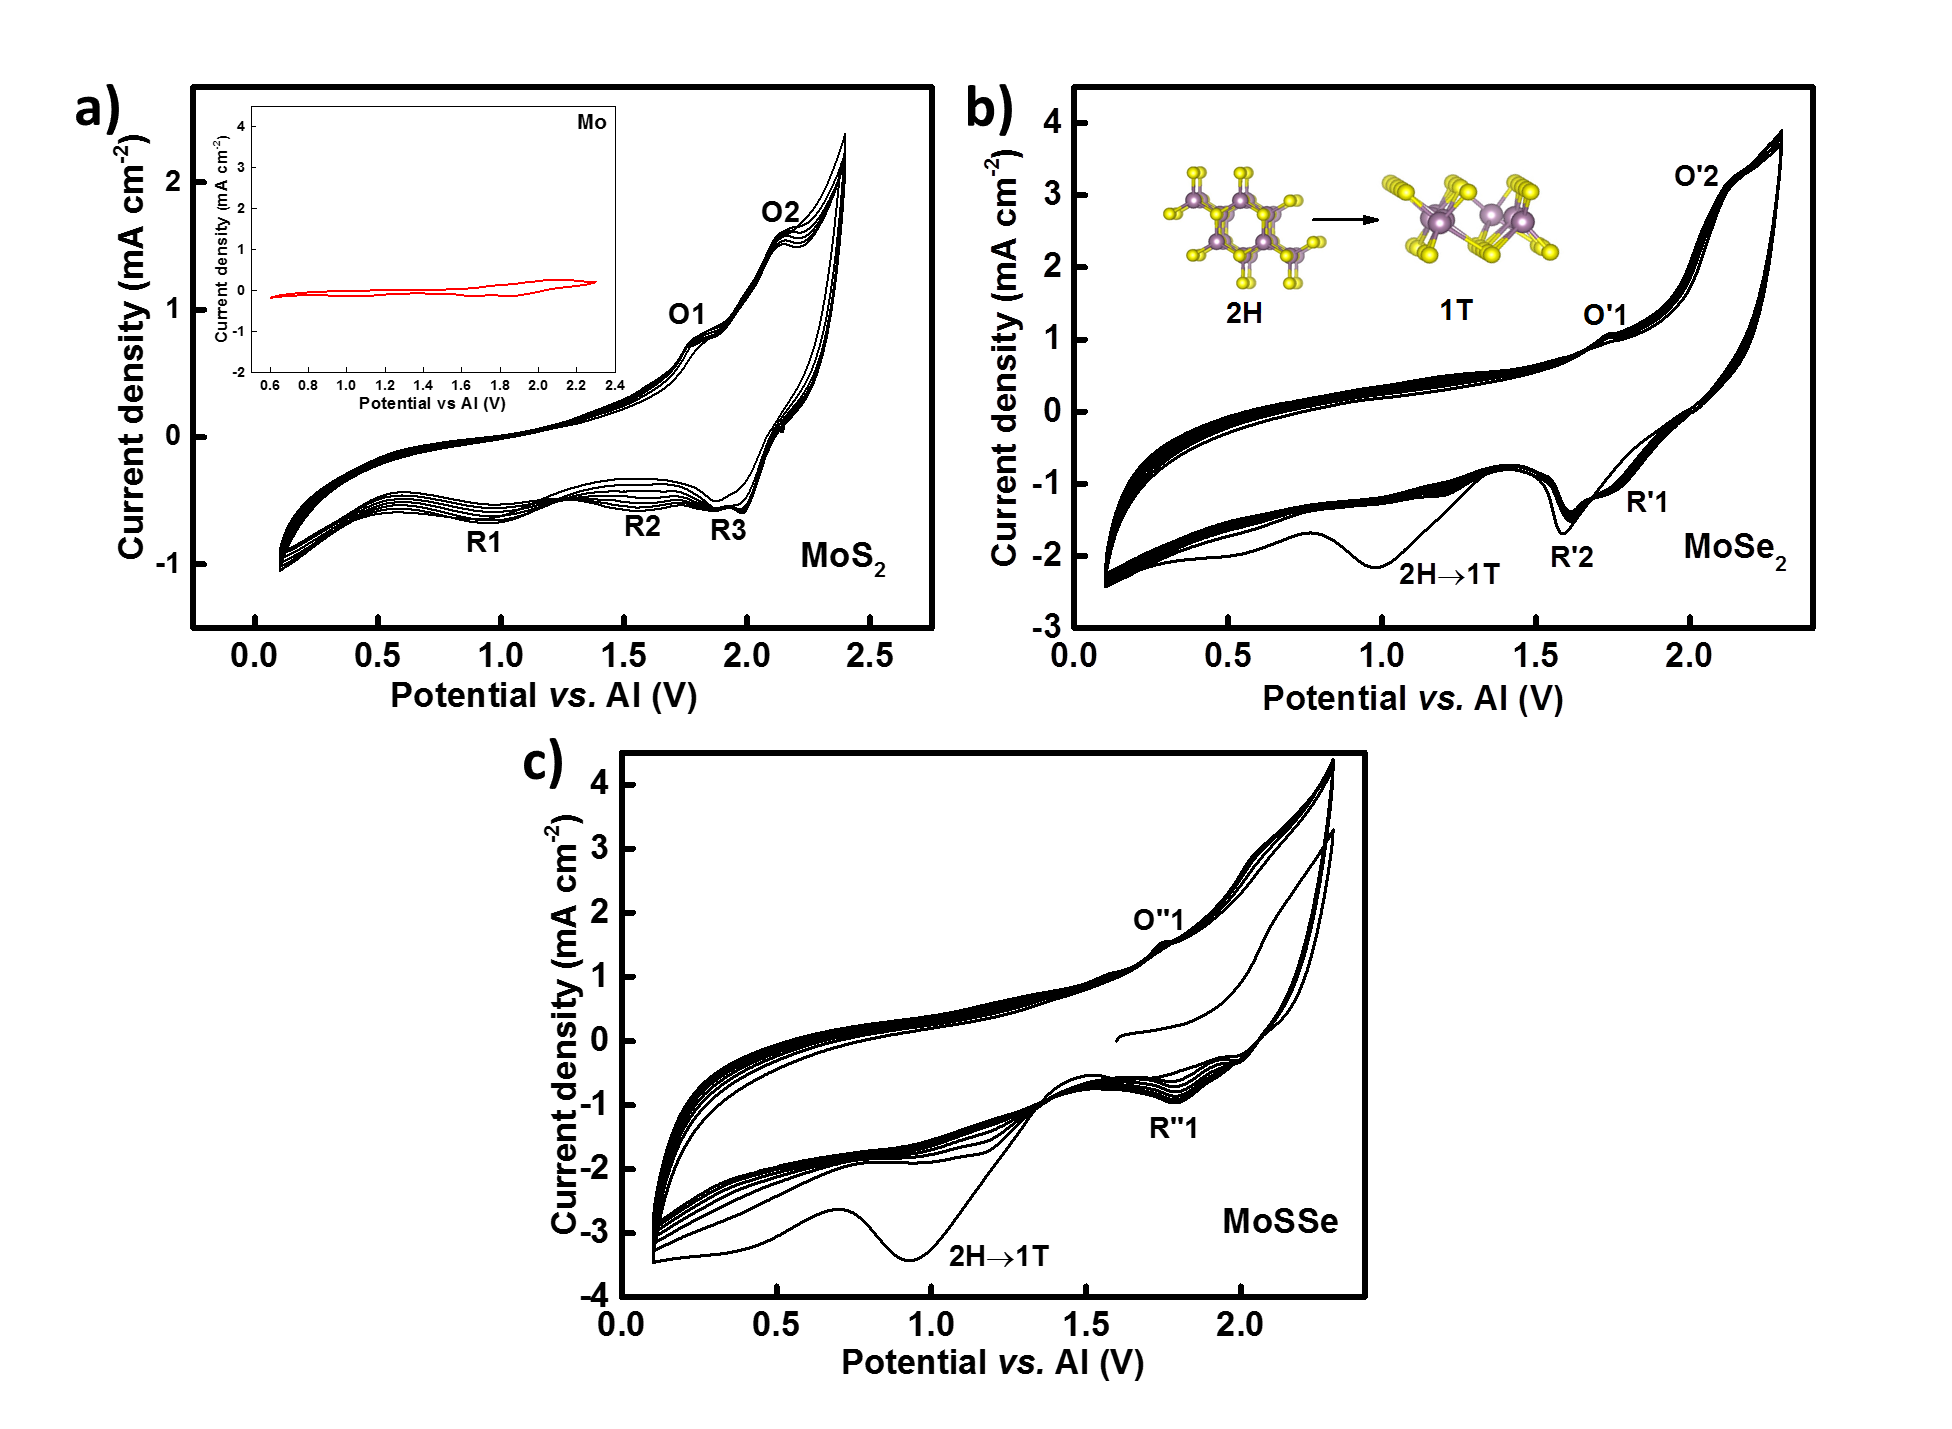
\includegraphics[width=\textwidth]{Figures/chap4fig/fig2}
  \caption{Cyclic voltammograms of a) \ce{MoS2}, b) \ce{MoSe2} and c) MoSSe at a scan rate of 10 mV s$^{-1}$ in a two-electrode aluminium-ion cell against an Al/\ce{Al^{3+}} reference electrode.}
  \label{Figures/chap4fig:fig2}
\end{figure} 

\begin{figure}
  \centering
  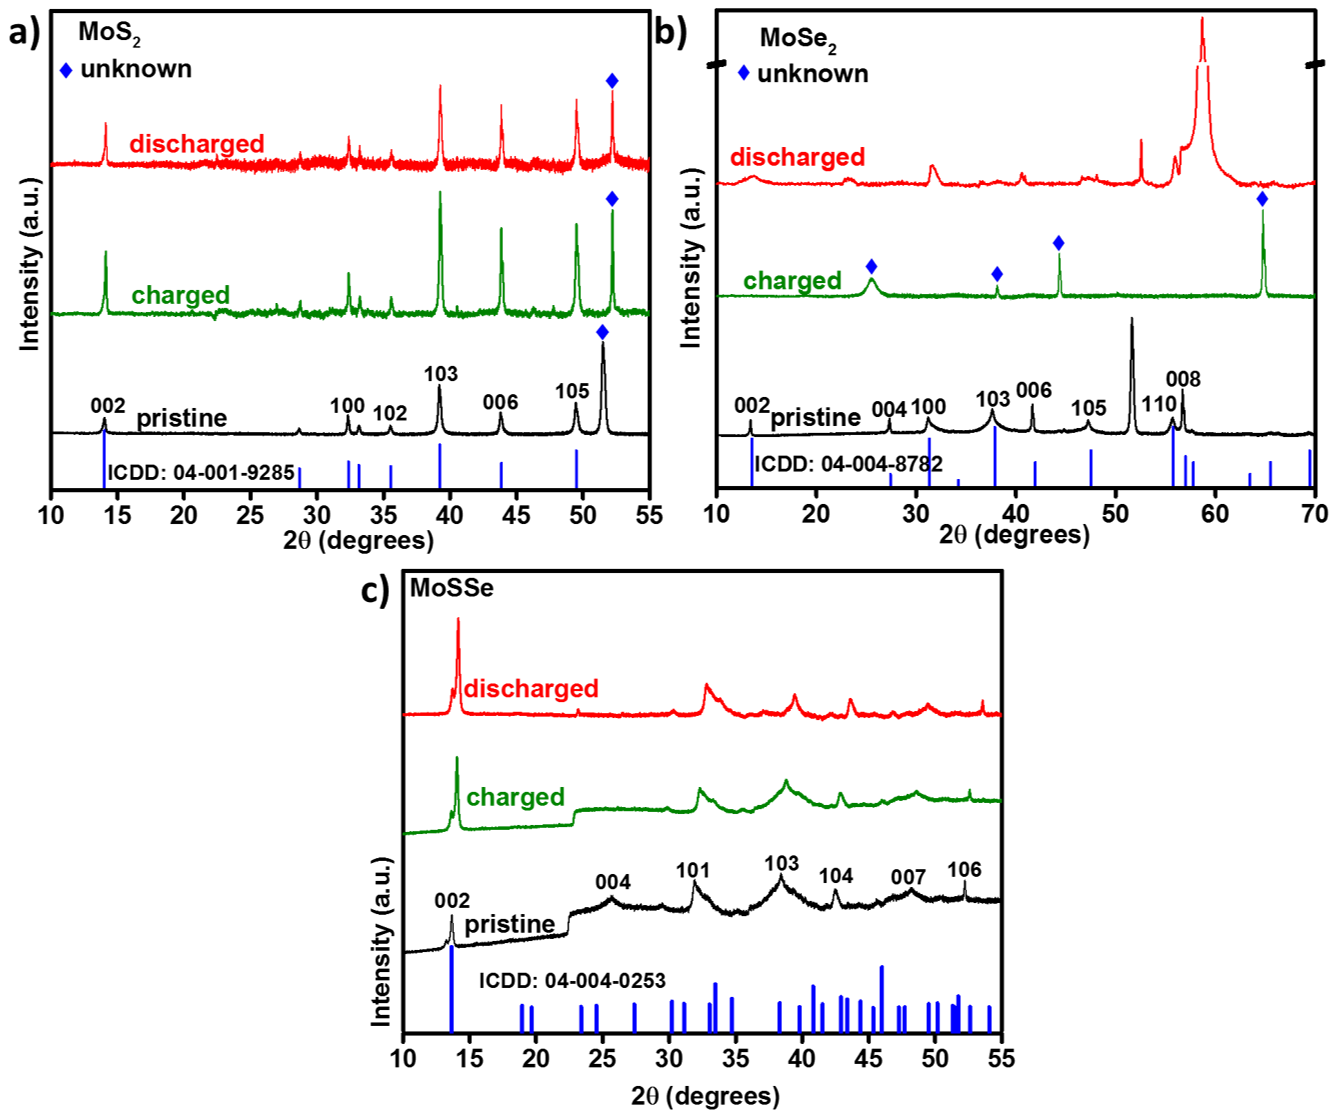
\includegraphics[width=\textwidth]{Figures/chap4fig/fig3}
  \caption{X-ray diffraction patterns of pristine (black), charged (green) and discharged (red) a) \ce{MoS2}, b) \ce{MoSe2} and c) MoSSe electrodes charged to 2.35 V and discharged to 0.2 V vs. Al/\ce{Al^{3+}}, with International Centre for Diffraction Data (ICDD) references.}
  \label{Figures/chap4fig:fig3}
\end{figure}

Figure \ref{Figures/chap4fig:fig3} shows the XRD patterns of \ce{MoS2}, \ce{MoSe2} and MoSSe electrodes. Pristine (in black), charged (in green) and discharged (in red) cathodes were compared after 30 cycles. \ce{MoS2} cells displayed a very small shift in their d-spacings. The peak at 14.2$^{\circ}$ (6.22 \AA) shifted to 14.02$^{\circ}$ (6.32 \AA), as shown in Figure \ref{Figures/chap4fig:fig3} a). Most of the peaks retained their positions after charge and discharge showing no significant change in the lattice dimensions. A completely different XRD pattern appeared after charging for Al/\ce{MoSe2} cells, as new peaks appeared at 2$\theta$ values, displayed in Figure \ref{Figures/chap4fig:fig3} b). After discharge, the diffraction patterns of the discharged cathodes resembled the pristine cathode patterns. Every time the cells were charged, \ce{MoSe2} seemed to adopt this new crystal lattice. However, the characteristic peaks of \ce{MoSe2} reappeared after discharge. This follows closely the observations made by Rani \textit{et al.} \cite{rani_fluorinated_2013}, where they proved intercalation of ions into the layers of fluorinated natural graphite during charging. This strongly confirms our hypothesis of a reversible intercalation taking place in \ce{MoSe2}. It was interesting to note that MoSSe did not have a well-defined crystal structure to begin with, Figure \ref{Figures/chap4fig:fig3} c). The patterns after charge and discharge did not look any different from the untested cathode. This confirmed MoSSe layers did not undergo any expansion and the initial specific capacities came from non-faradaic reactions where \ce{AlCl4-} might have been electrostatically absorbed and desorbed onto the surface of the electrode.  

To further understand the interactions between \ce{AlCl4-} and \ce{MoSe2} we used XPS, which is a useful method for distinguishing various oxidation states and helps in identifying different polymorphs (2H and 1T) \cite{fan_hybrid_2017}. The detailed narrow spectrum scans in Figure \ref{Figures/chap4fig:MoAlOverallMoSeMoSSe} show the binding energies of Mo (3d$_{5/2}$ and 3d$_{3/2}$, Figure \ref{Figures/chap4fig:MoAlOverallMoSeMoSSe} a) and b)) and Al 2p peaks for charged \ce{MoSe2} (Figure \ref{Figures/chap4fig:MoAlOverallMoSeMoSSe} c)) and MoSSe electrodes (Figure \ref{Figures/chap4fig:MoAlOverallMoSeMoSSe} d)). In pristine \ce{MoSe2}, two peaks appeared at 229.1 eV and 232.2 eV corresponding to 3d$_{5/2}$ and 3d$_{3/2}$ (Figure\ \ref{Figures/chap4fig:MoSeSeAlClPrtChg} a)). Selenium displayed a doublet at 55.4 eV and 54.6 eV corresponding to Se 3d$_{3/2}$ and 3d$_{5/2}$ respectively (Figure \ref{Figures/chap4fig:MoSeSeAlClPrtChg} c)). Peak splitting in an XPS spectrum can indicate a phase change or a change in oxidation state. After charge, the peak for Mo 3d split into three doublets indicating the presence of multiple oxidation states or phases of Mo (Figure \ref{Figures/chap4fig:MoAlOverallMoSeMoSSe} a)). Se 3d deconvoluted into four peaks after charge, Figure \ref{Figures/chap4fig:MoSeSeAlClPrtChg} e), confirming presence of more than one phase after charge. This was similar to observations made by Fan \textit{et al.} Pristine electrodes of MoSSe contained Mo in more than one oxidation state, and provided evidence for the presence of both 2H and 1T polymorphs, Figure\ \ref{Figures/chap4fig:MoSeSeAlClPrtChg} b). After charging, the width of peaks at 231.7 eV (Mo 3d$_{5/2}$) and 228.6 eV (Mo 3d$_{3/2}$) increased as displayed in Figure\ \ref{Figures/chap4fig:MoAlOverallMoSeMoSSe} b). After comparing Figure\ \ref{Figures/chap4fig:MoSeSeAlClPrtChg} d) and f), we noticed that the Se 3d spectrum deconvoluted into four peaks after charging in MoSSe cells. An increase in the peak width was observed for both Mo and Se binding energies. A new peak at $\sim$236 eV in Mo 3d spectra for \ce{MoS2}, \ce{MoSe2} and MoSSe electrodes generally indicates a Mo$^{6+}$ species present in molybdenum oxide, \ce{MoO3}. 

\begin{figure}
  \centering
  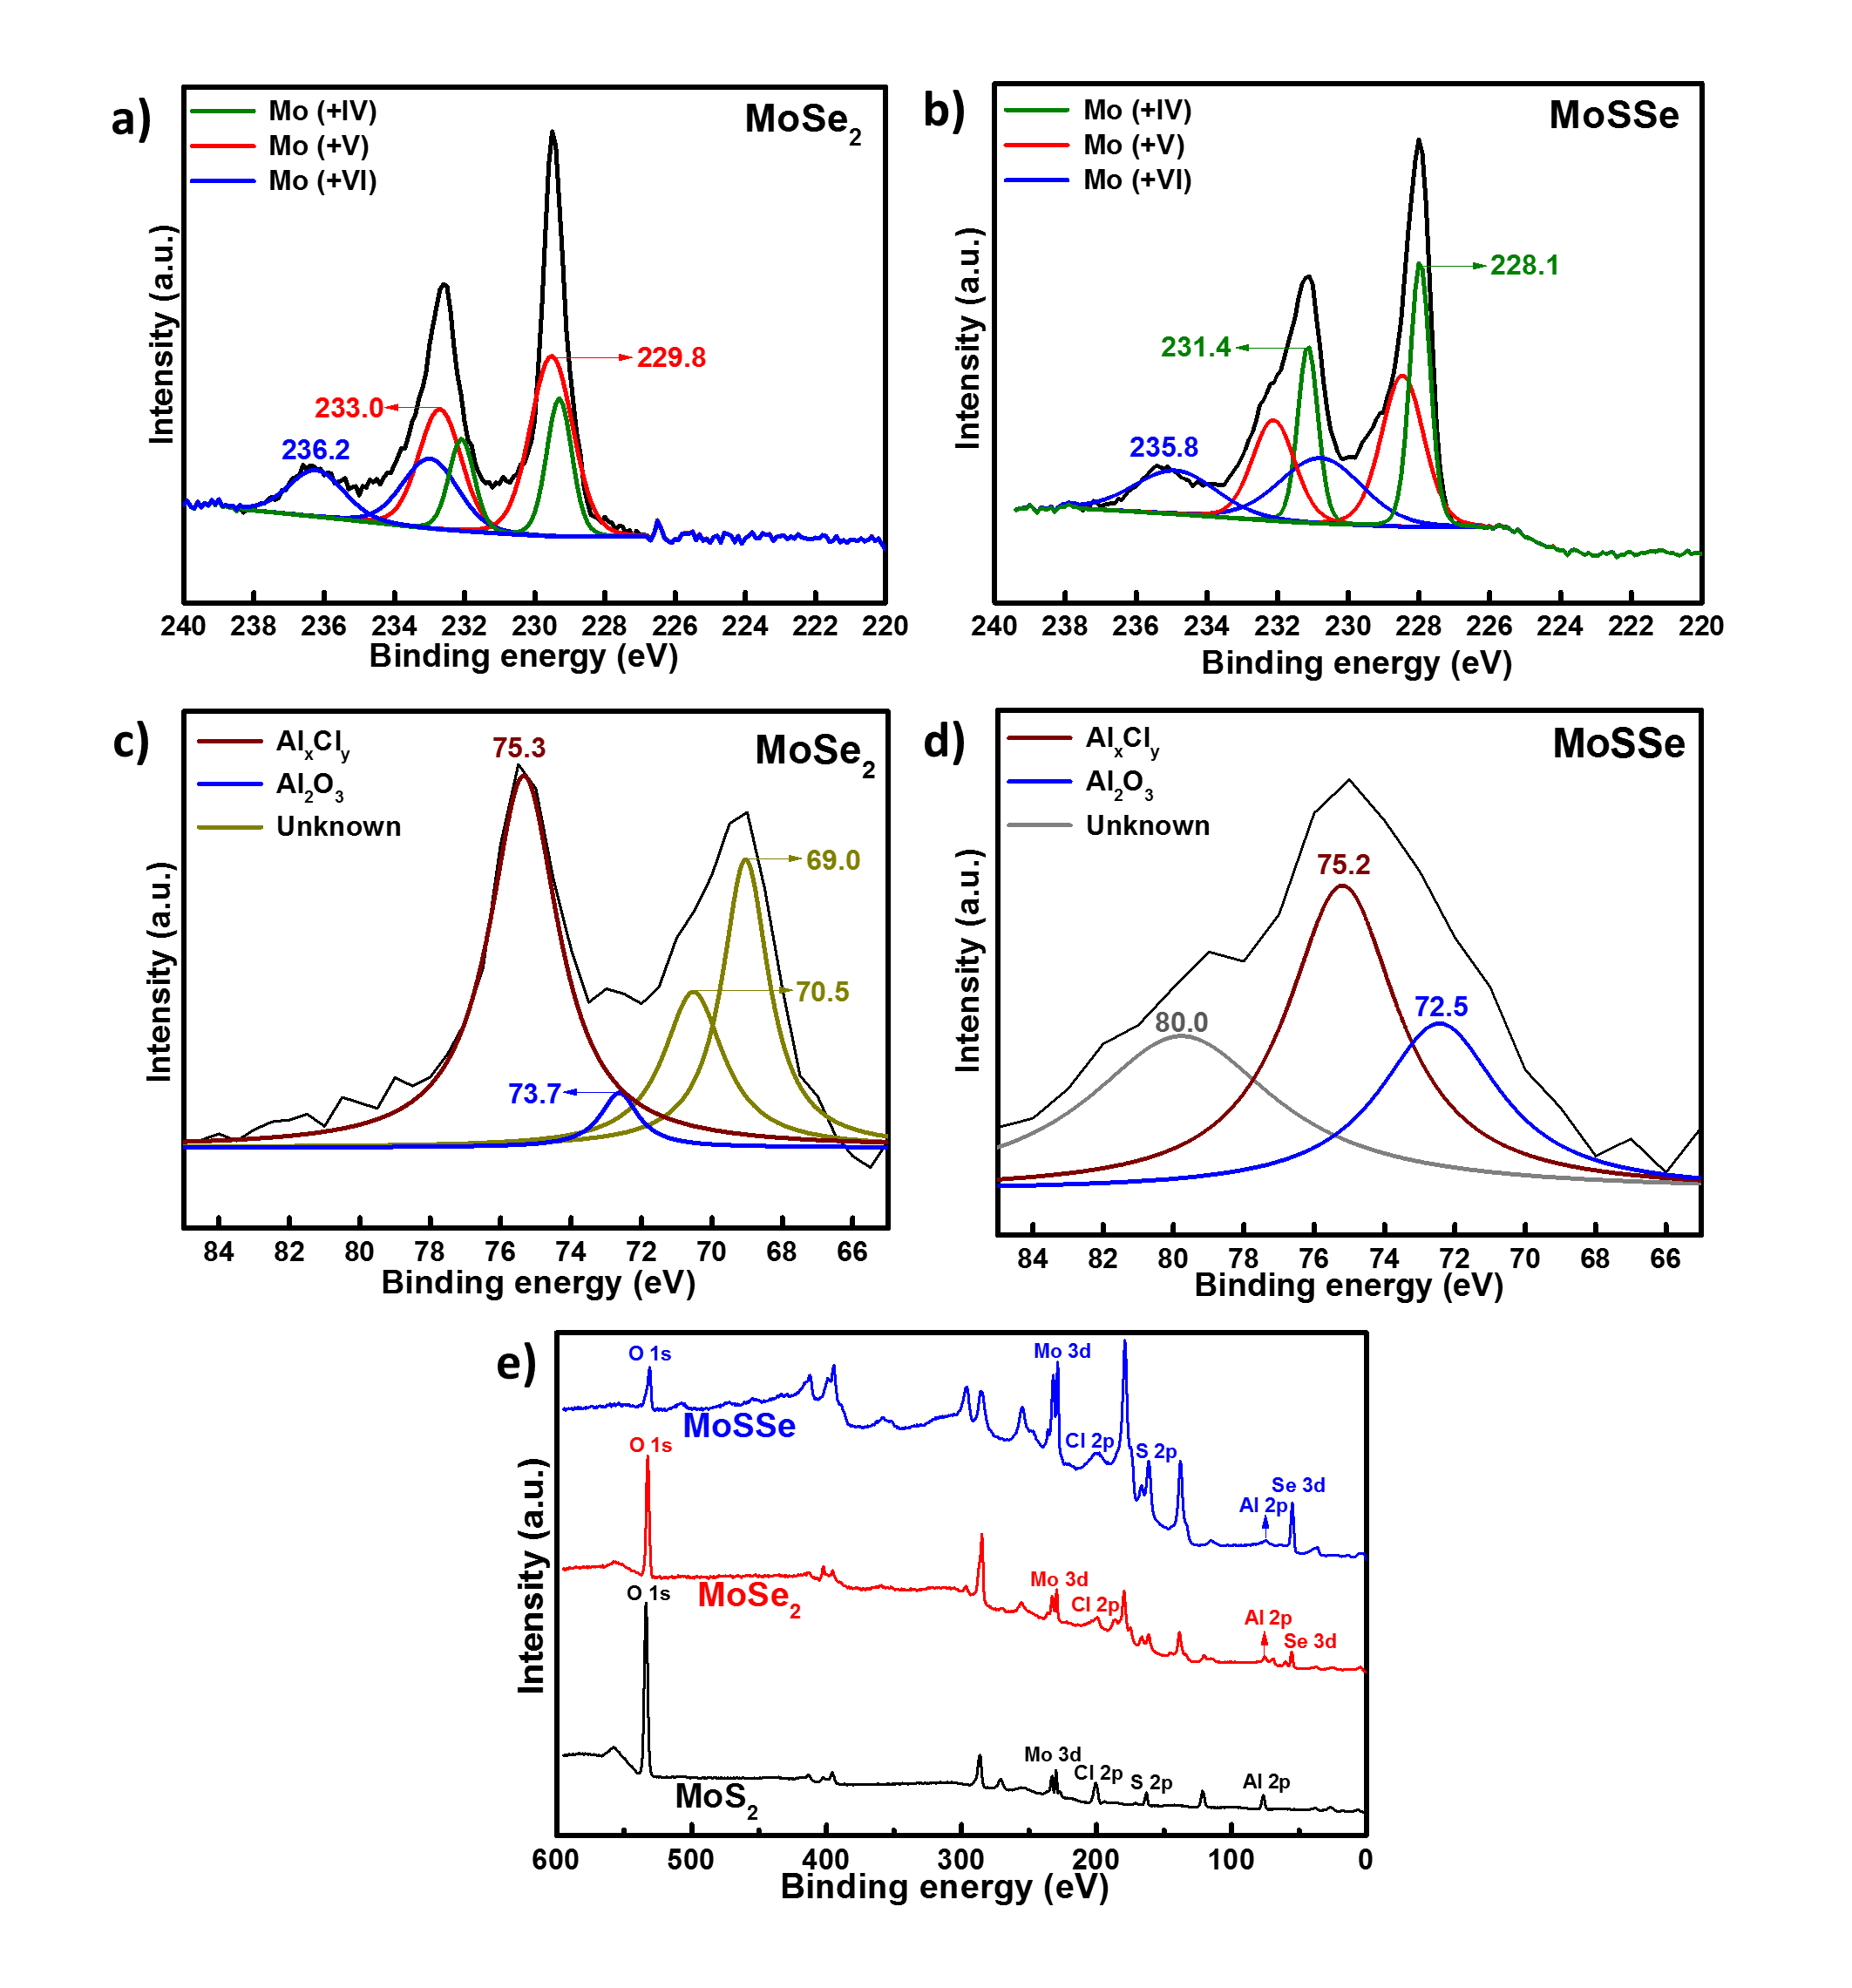
\includegraphics[width=\textwidth]{Figures/chap4fig/MoAlOverallMoSeMoSSe}
  \caption{XPS spectra of Mo 3d orbitals in a charged a) \ce{MoSe2} and b) MoSSe cathode and Al 2p orbitals in a charged c) \ce{MoSe2} and d) MoSSe cathode. e) An overview spectrum of all three tested and charged cathodes.}
  \label{Figures/chap4fig:MoAlOverallMoSeMoSSe}
\end{figure}

The peak shifts detected in Mo 3d spectra for charged \ce{MoS2} and \ce{MoSe2} cathodes were insignificant in MoSSe (cf.\ Figures \ref{Figures/chap4fig:MoS2XPS} a), b), \ref{Figures/chap4fig:MoAlOverallMoSeMoSSe} a), and \ref{Figures/chap4fig:MoSeSeAlClPrtChg} a)). This further confirms the absence of redox reactions and that the capacity was mainly derived from a surface-based charge storage. As expected, charged electrodes showed higher concentration of aluminium and chlorine than discharged electrodes as seen in Figure \ref{Figures/chap4fig:MoSeSeAlClPrtChg} g) and h). The XPS spectra support the observation that \ce{MoSe2} underwent a phase transformation that made it a better performing cathode than \ce{MoS2}. Further analysis is needed to fully understand the mechanism of MoSSe.

\begin{figure}
  \centering
  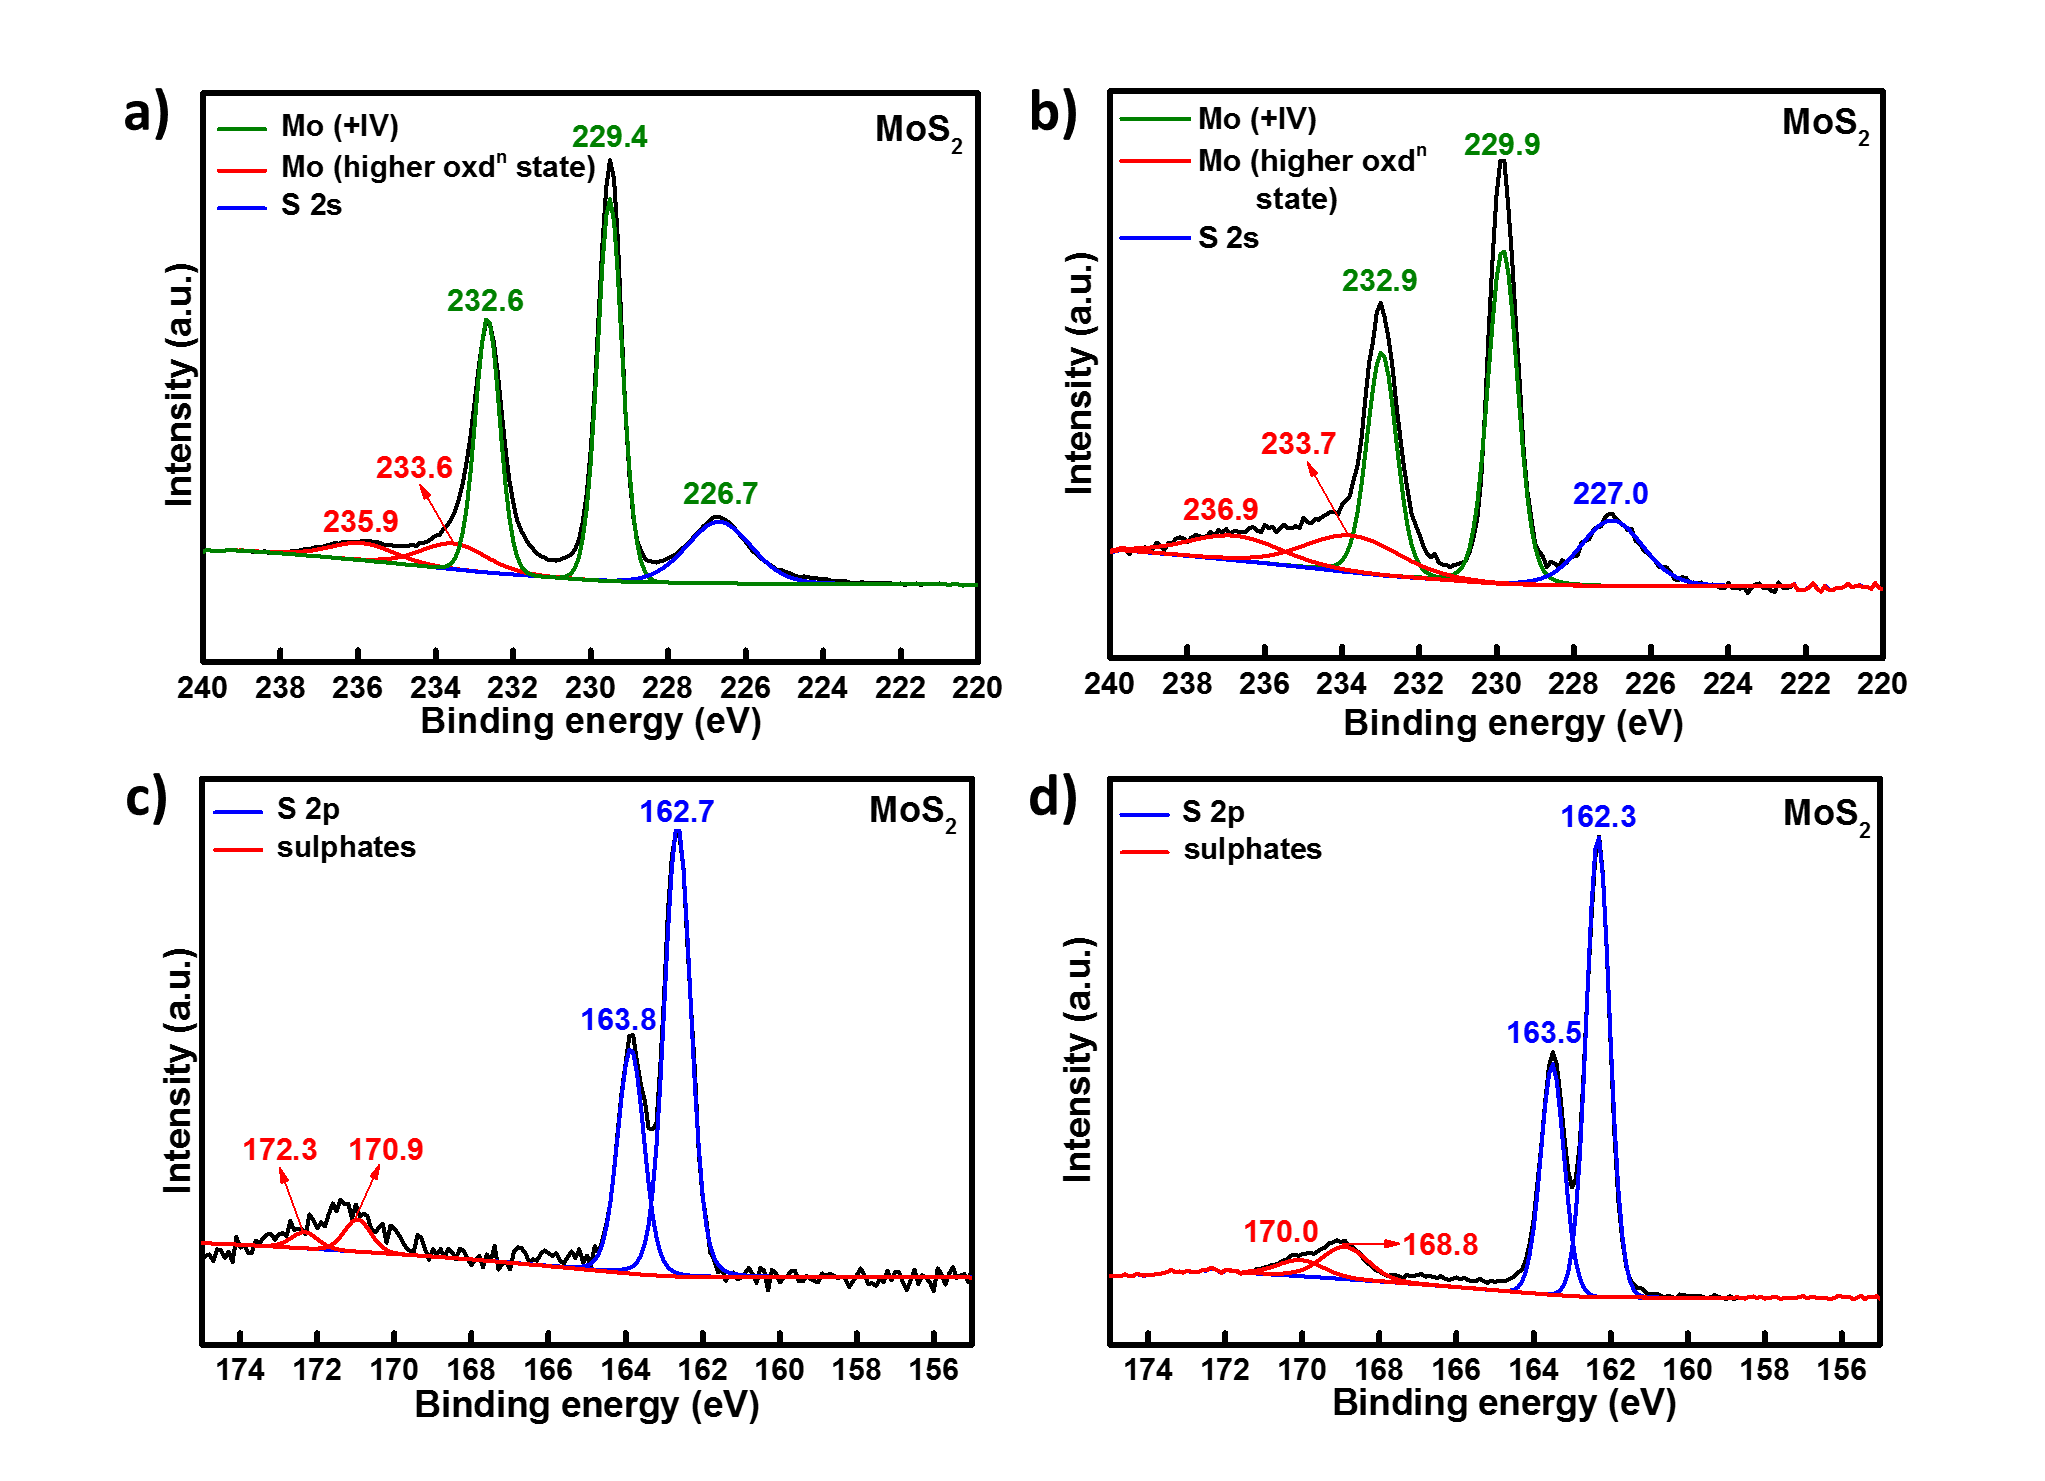
\includegraphics[width=\textwidth]{Figures/chap4fig/MoS2XPS}
  \caption{XPS spectra of Mo 3d orbitals in a charged and b) discharged \ce{MoS2} cathode and binding energies of S 2p orbital in a charged and b) discharged \ce{MoS2} cathode.}
  \label{Figures/chap4fig:MoS2XPS}
\end{figure}

\begin{figure}
  \centering
  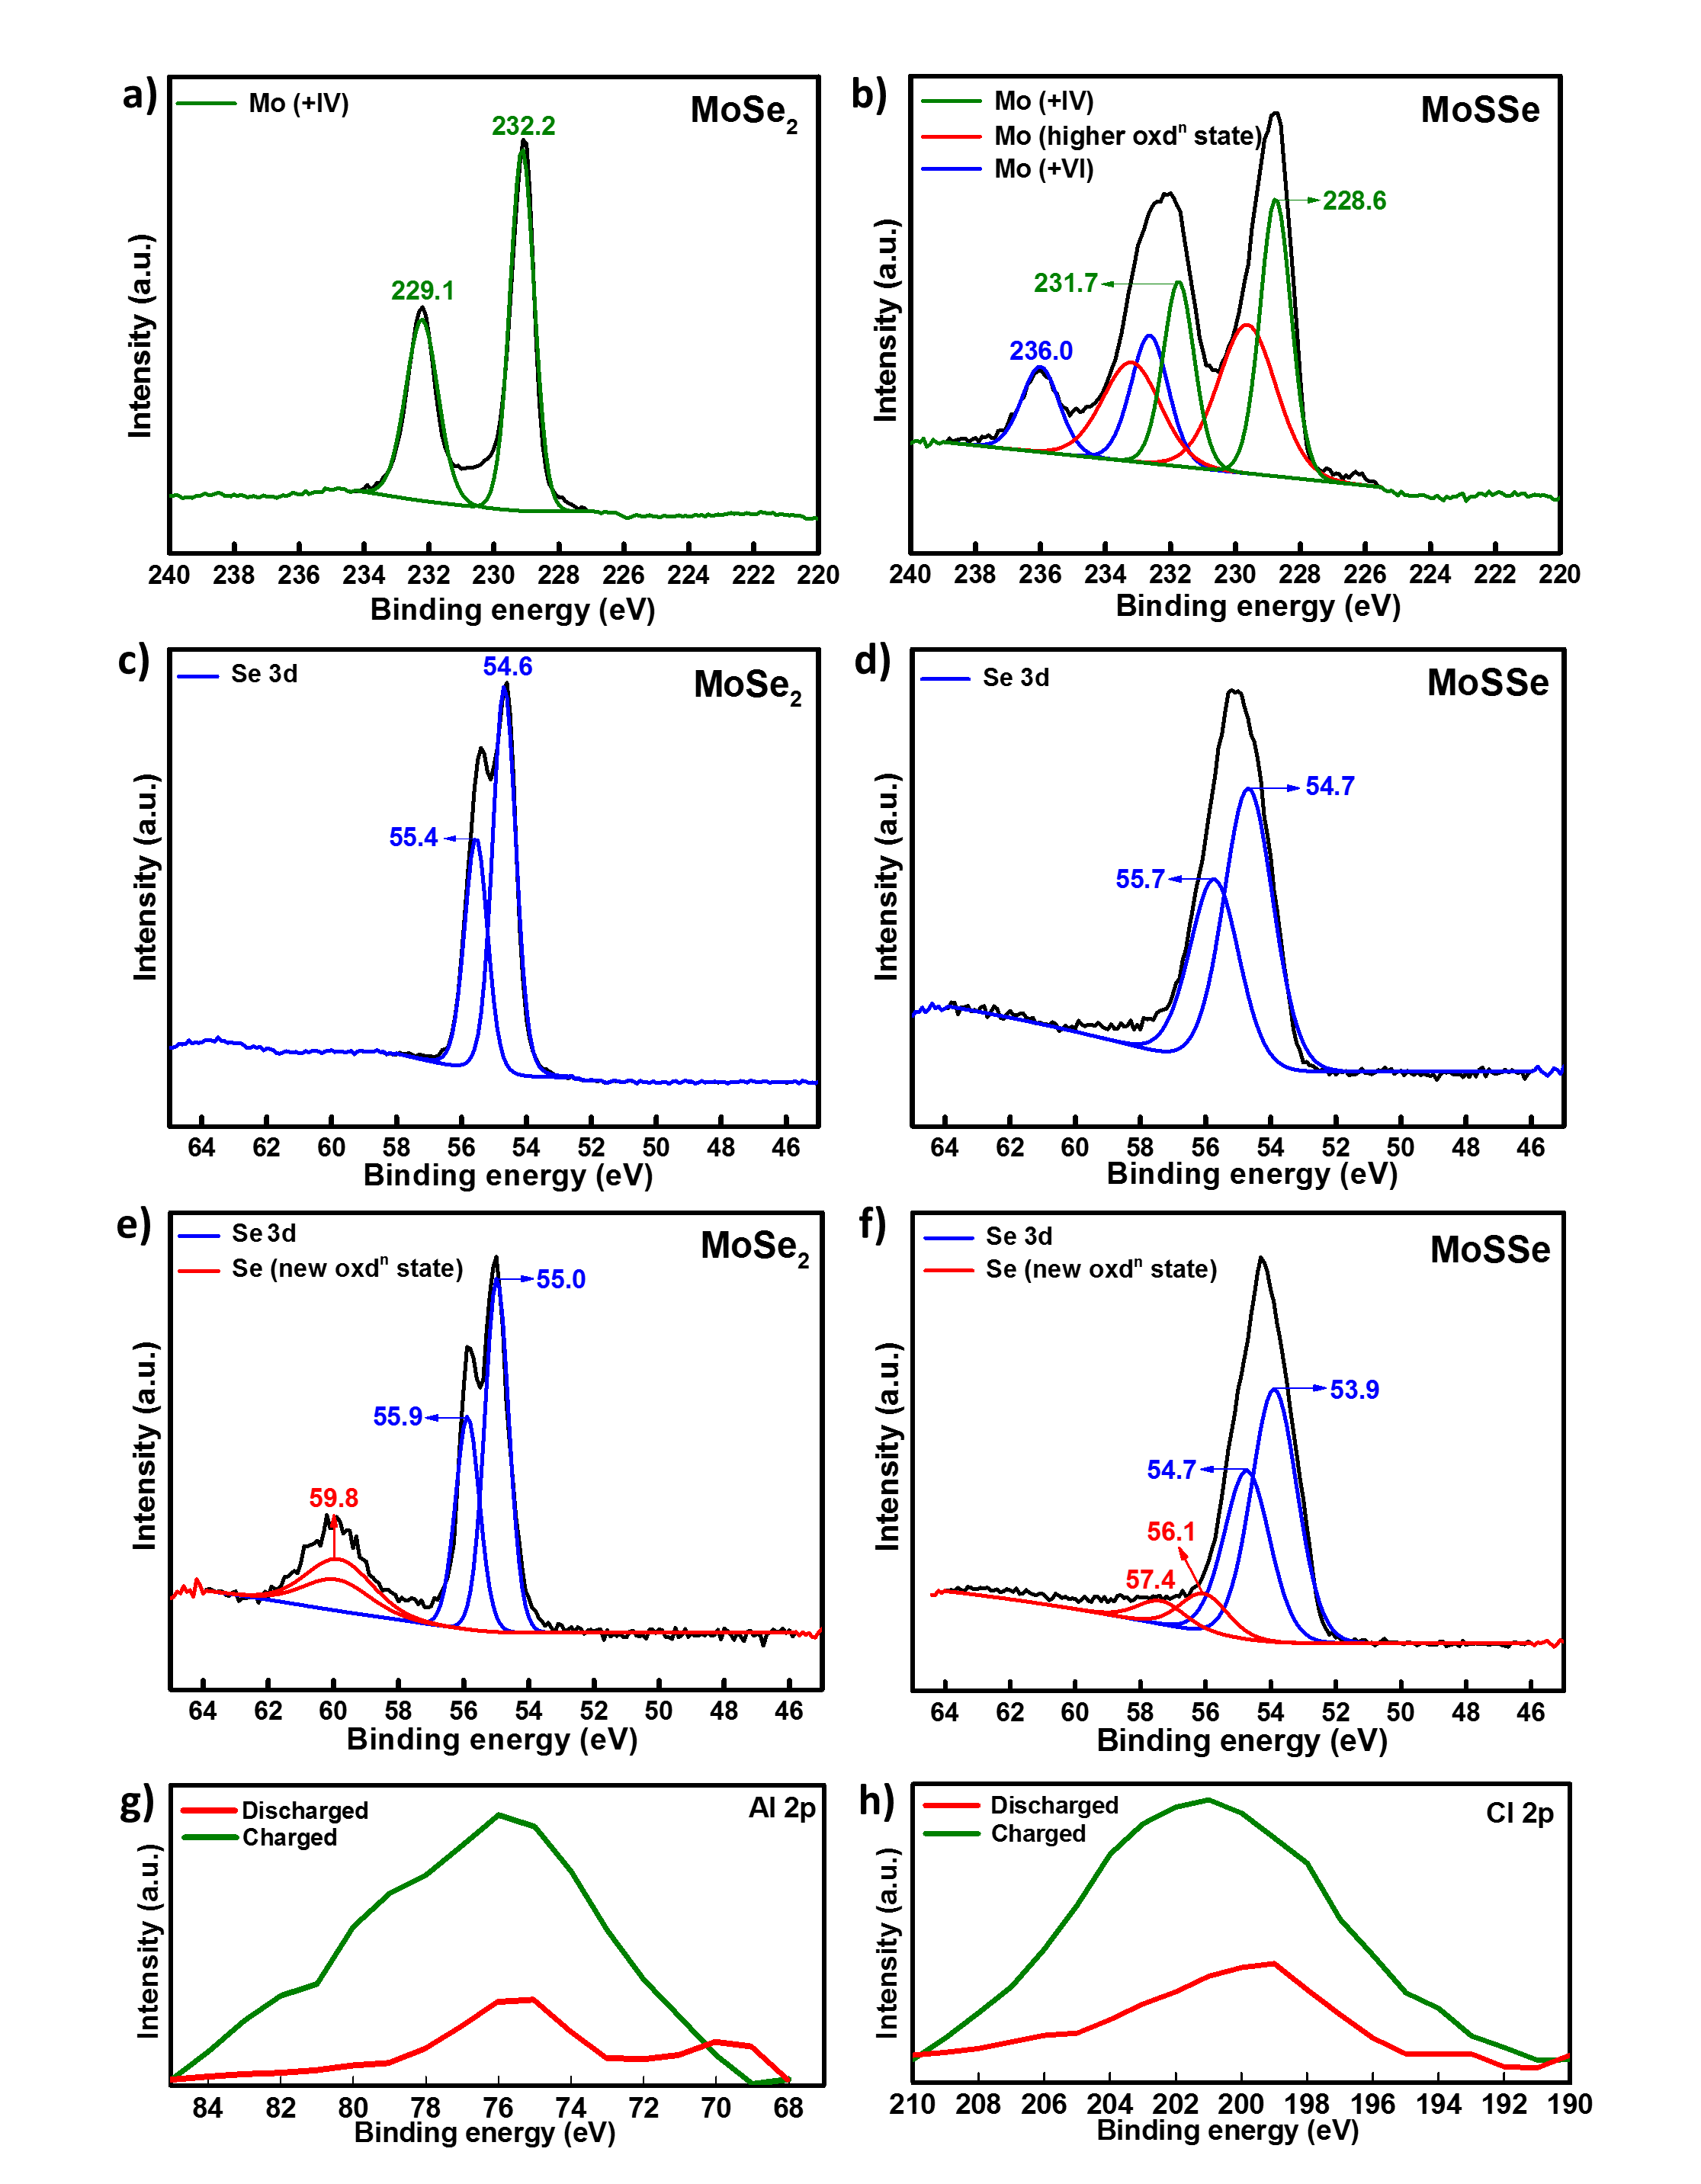
\includegraphics[width=\textwidth]{Figures/chap4fig/MoSeSeAlClPrtChg}
  \caption{XPS spectra of Mo 3d for pristine a) \ce{MoSe2} and b) MoSSe electrodes. The spectra of \ce{MoSe2} are composed of two peaks at 232.2 eV and 229.1 eV corresponding to \ce{Mo^{4+}}. MoSSe spectra consist of three doublet bands, which were assigned to \ce{Mo^{4+}}, one with higher oxidation state and another band corresponding to \ce{Mo^{6+}} at 236 eV. c) Pristine and e) charged Se 3d from \ce{MoSe2}. \ce{MoSe2} observed peaks corresponding to 3d$_{3/2}$ and 3d$_{5/2}$ at 55.6 eV and 54.6 eV respectively. Binding energies of Se 3d from d) pristine and f) charged MoSSe cathodes.}
  \label{Figures/chap4fig:MoSeSeAlClPrtChg}
\end{figure}

Charged \ce{MoSe2} electrodes displayed binding energies of Al 2p at 77 eV (red) and 76 eV (in blue) corresponding to chlorides (\ce{AlxCly}) and \ce{Al2O3} respectively in Figure \ref{Figures/chap4fig:MoAlOverallMoSeMoSSe} c). New peaks were observed at much lower binding energies --- 69 and 70 eV (green) suggesting the presence of a new complex with an increased electron density around aluminium. An overall spectra of charged \ce{MoS2}, \ce{MoSe2} and MoSSe cathodes is shown in Figure \ref{Figures/chap4fig:MoAlOverallMoSeMoSSe} e) indicating the presence of Al and Cl (from chloroaluminates) and oxygen (from \ce{MoO3}).

In addition, we compared the Raman spectra of pristine and charged cathodes to detect shifts in vibrational modes, Figure \ref{Figures/chap4fig:fig5}. E$^1_{2g}$ and A$^1_g$ are the most intense vibrational modes for molybdenum dichalcogenides \cite{yang_pressure-induced_2019, r_2d_2017,sharma_stable_2018}. Peaks corresponding to E$^1_{2g}$ and A$^1_g$ modes for \ce{MoS2} (Figure \ref{Figures/chap4fig:fig5} a)) are prominent at 384.6 cm$^{-1}$ and 410.2 cm$^{-1}$ respectively. A$^1_g$ indicates an out-of-plane symmetric displacement of S atoms, whereas E$^1_{2g}$ suggests an in-layer displacement. Also, separation between the two peaks indicates a multi-layer structure, which was observed for all three materials. No significant peak shift or peak broadening was observed for the charged \ce{MoS2} electrode. For 2H \ce{MoSe2} (Figure \ref{Figures/chap4fig:fig5} b)), A$^1_g$ is the most intense vibration occurring at a frequency lower than that of E$^1_{2g}$. When the number of layers decreases, the A$^1_g$ mode softens (increase in full-width-at-half-maximum (FWHM)). Spectra generated after intercalation were different from the pristine cathodes because phase conversion from 2H to 1T decreases the molecule's symmetry and more Raman bands get active. The presence of J1 and J2 peaks in addition to E$^1_{2g}$ and A$^1_g$ at lower wavelengths suggest the existence of 1T phase especially for \ce{MoSe2} and MoSSe (inset, Figure\ \ref{Figures/chap4fig:fig5} b) and c)). This agrees with our CV scans where a phase transition was observed for \ce{MoSe2} and MoSSe. Raman results suggest that 'chloroalumination' or insertion of chloroaluminates changed the symmetry and vibrational modes of \ce{MoSe2}'s crystal lattice. 

\begin{figure}
  \centering
  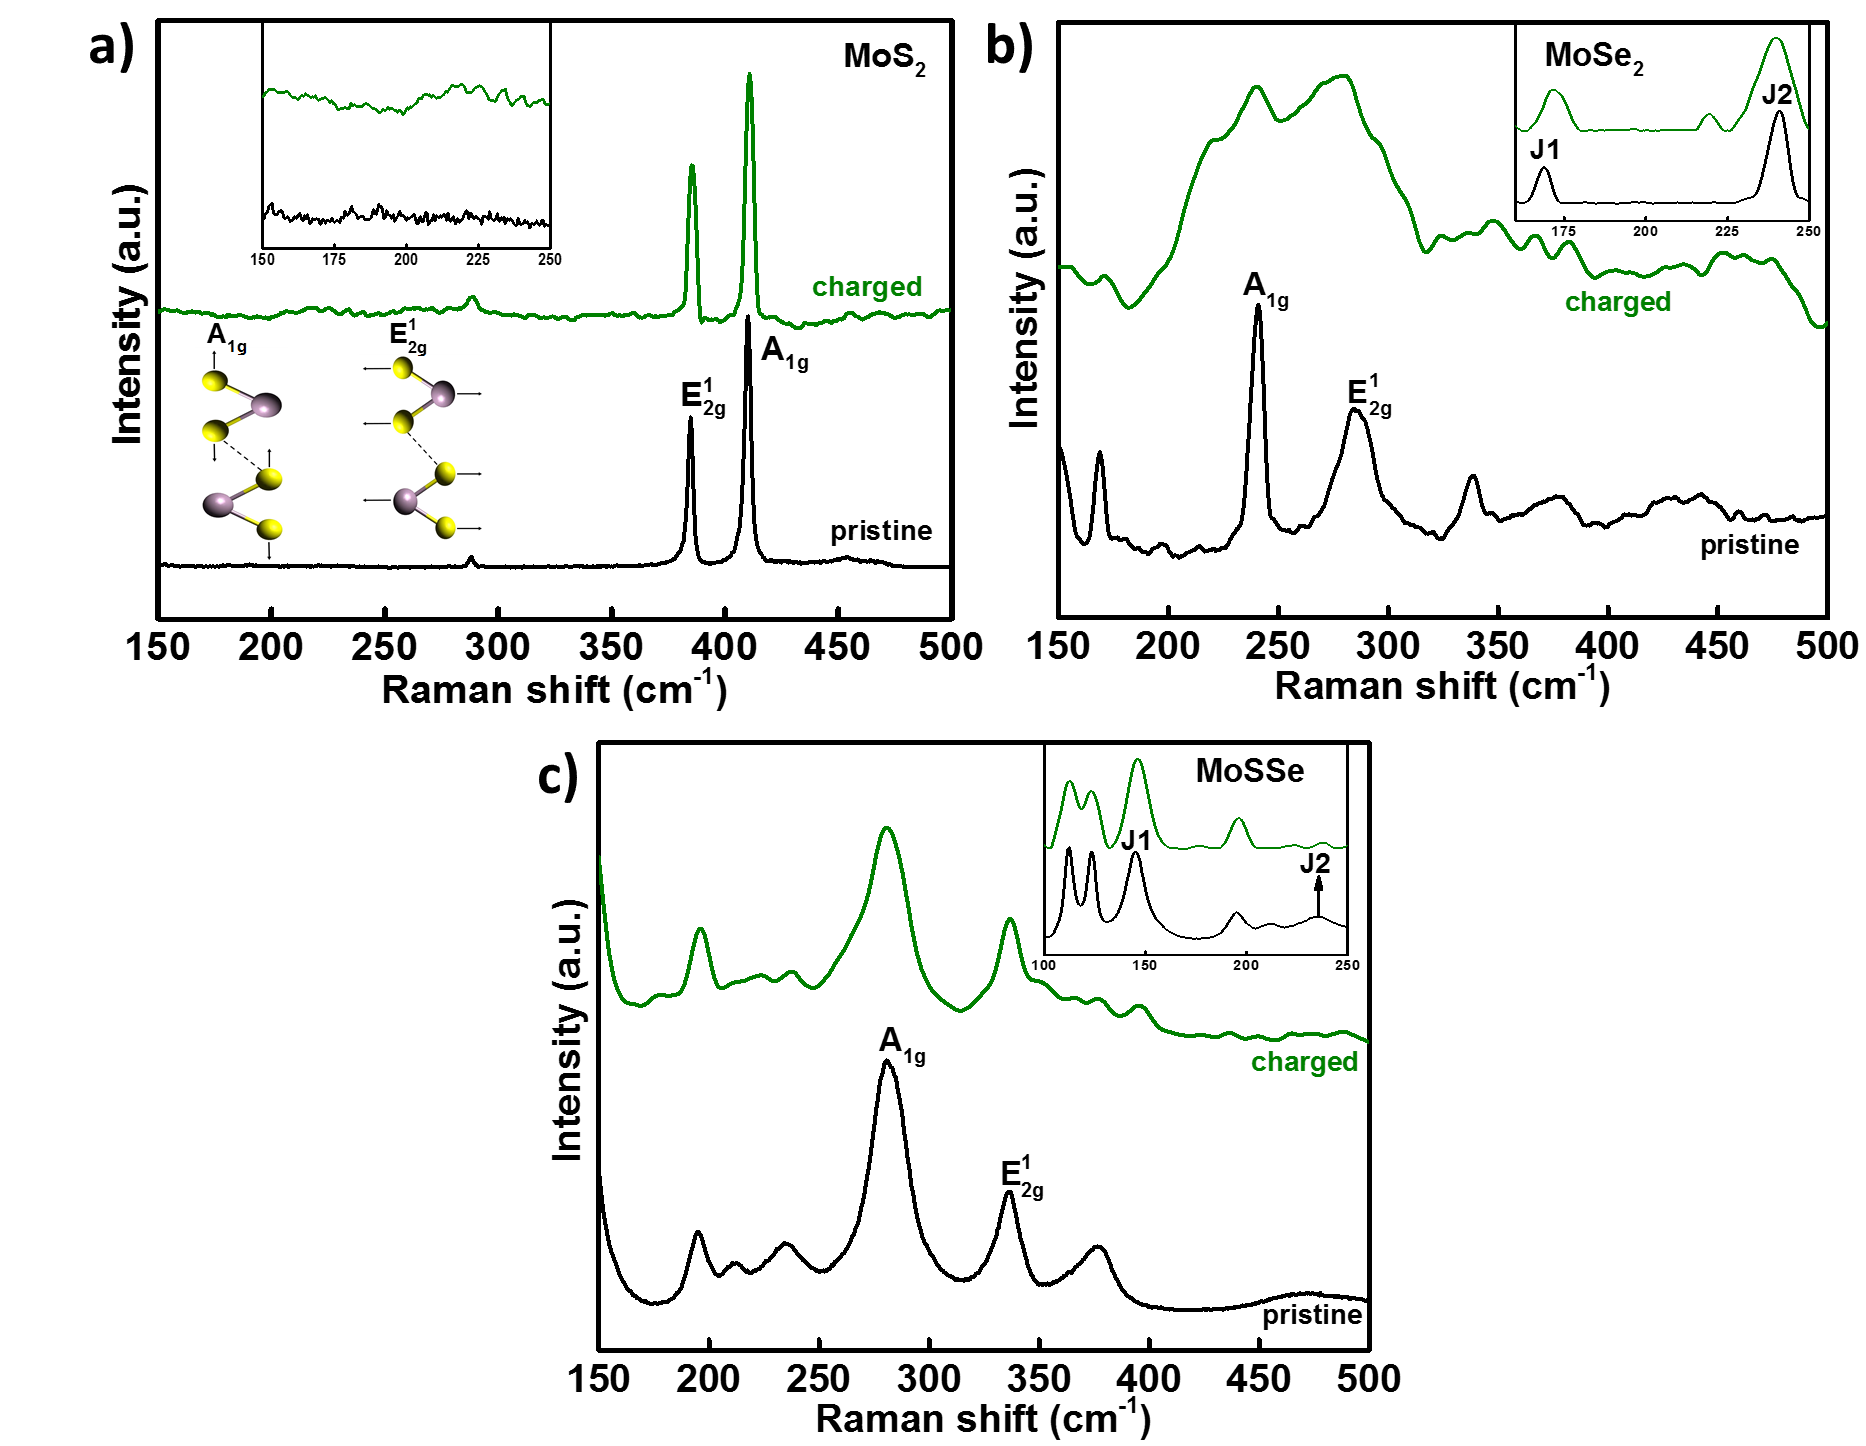
\includegraphics[width=\textwidth]{Figures/chap4fig/fig5}
  \caption{Raman spectra of pristine (black) and charged (green) a)\ce{MoS2}, b) \ce{MoSe2} and c) MoSSe electrodes with position of new Raman active J1 and J2 bands marked along with E$^1_{2g}$ and A$^1_g$ bands.}
  \label{Figures/chap4fig:fig5}
\end{figure}

\begin{figure}
  \centering
  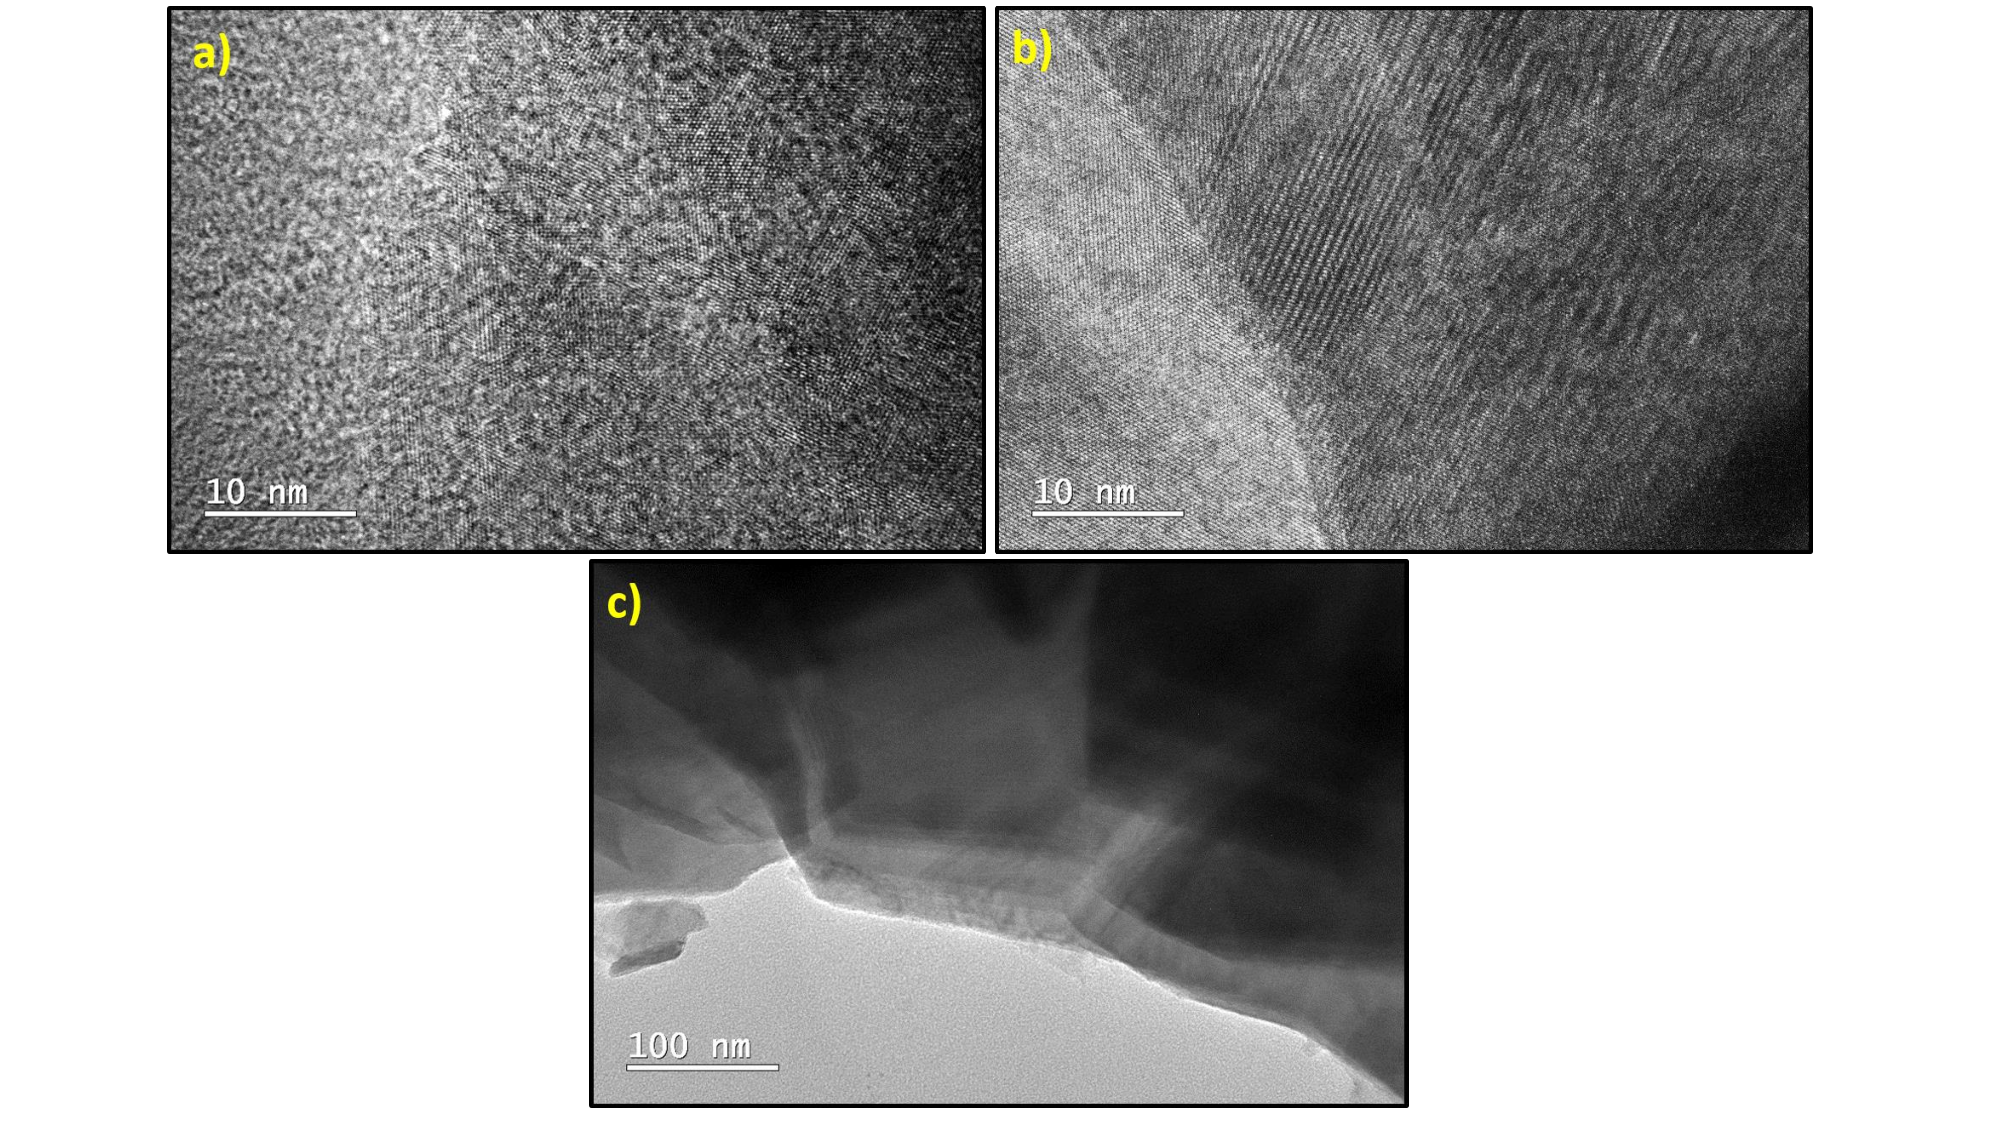
\includegraphics[width=\textwidth]{Figures/chap4fig/mose2tem}
  \caption{Raman spectra of pristine (black) and charged (green) a)\ce{MoS2}, b) \ce{MoSe2} and c) MoSSe electrodes with position of new Raman active J1 and J2 bands marked along with E$^1_{2g}$ and A$^1_g$ bands.}
  \label{Figures/chap4fig:mose2tem}
\end{figure}
 
%\chapter{Carbon-based cathodes for reachargeable AIBs} % Main chapter title
In this chapter, we discuss performance of AIBs using carbon-based materials as cathodes and establish their individual mechanism.
\label{chap5} % For referencing the chapter elsewhere, use \ref{Chapter1} 

%----------------------------------------------------------------------------------------

% Define some commands to keep the formatting separated from the content 
\newcommand{\keyword}[1]{\textbf{#1}}
\newcommand{\tabhead}[1]{\textbf{#1}}
\newcommand{\code}[1]{\texttt{#1}}
\newcommand{\file}[1]{\texttt{\bfseries#1}}
\newcommand{\option}[1]{\texttt{\itshape#1}}
 In this work, we compare four different forms of carbon: activated carbon from human hair (ACH), hemp fibers, a fullerene extract (CFEx) and Super-P carbon black as cathodes for non-aqueous aluminium-ion batteries. These materials differ in their general structure, porosity and morphology. The fullerenes display a crystalline structure, whereas hemp fibers, Super-P and ACH are amorphous in nature. Of all materials, ACH recorded the highest specific capacity after 50 cycles at 103 mAh g$^{-1}$ with a coulombic efficiency of ~90\% at a current rate of 50 mV s$^{-1}$. Both hemp fibers and SPC achieved their highest specific capacities at 56 mAh g-1 and 84 mAh g$^{-1}$ respectively. CFEx, a mixture of \ce{C60} (85\%) and \ce{C70} (15\%) fullerene, recorded its highest capacity at 78 mAh g$^{-1}$ and maintained it for 50 cycles. The cells were charged and discharged to 2.45 V and 0.2 V respectively. 
\section{Theory and background}
Different varieties of carbon-based materials have been widely used in energy storage applications. Graphite, with its layered structure turned out to be an ideal intercalation cathode material \cite{ji_recent_2011, yoo_large_2008, lian_large_2010}. Activated carbon, owing to its porous structure, provided a high surface area for absorption of electrolyte ions in super-capacitors \cite{eliad_ion_2001, zhu_carbon-based_2011-2}. Aluminium-ion batteries (AIBs) use low-cost, abundant materials, a non-flammable electrolyte and aim to provide higher theoretical energy density than lithium-ion batteries (LIBs) due to the multivalent nature of aluminium. Exhaustive use of lithium and cobalt in LIBs would make portable batteries expensive in the coming years. One needs to switch to cost-effective alternatives. The above-mentioned properties make AIBs an interesting alternative\cite{ambroz_trends_2017-1}. We tested a number of rechargeable AIBs using an ionic liquid electrolyte with carbon-based cathodes.
Graphite has been commonly used as a cathode in AIBs. It has a) a layered structure that enhances the intercalation process, b) good conductivity and c) a high electrical potential {\it vs.} \ce{Al}/\ce{Al^{3+}} of 2.1 V. Various forms of graphite such as fluorinated graphite \cite{rani_fluorinated_2013}, kish graphite flakes \cite{wang_kish_2017-1}, three-dimensional graphitic-foam\cite{wu_3d_2016}, graphene aerogels\cite{huang_graphene_2019} and several other forms have been tested as cathodes for AIBs, which showed specific capacities ranging from 60-250 mAh g$^{-1}$. The \ce{AlCl4-}-anions intercalate into the graphitic stacks when the cell is being charged and deintercalate during discharge. X-ray diffraction (XRD) and Raman spectroscopy studies have widely been used to establish this mechanism\cite{rani_fluorinated_2013, wang_advanced_2017, lin_ultrafast_2015-3} as shown in Figure \ref{Figures/chap5fig:graphmech}. Raman data showed that conversion of a doublet peak during charge to one single peak after the cell was fully charged, indicated two stages of intercalation. XPS studies confirmed reversible oxidation/reduction of carbon when \ce{AlCl4-} anions intercalate/deintercalate respectively\cite{stadie_zeolite-templated_2017, liu_binder-free_2019}.
 \begin{figure}[tbh!]
  \centering
  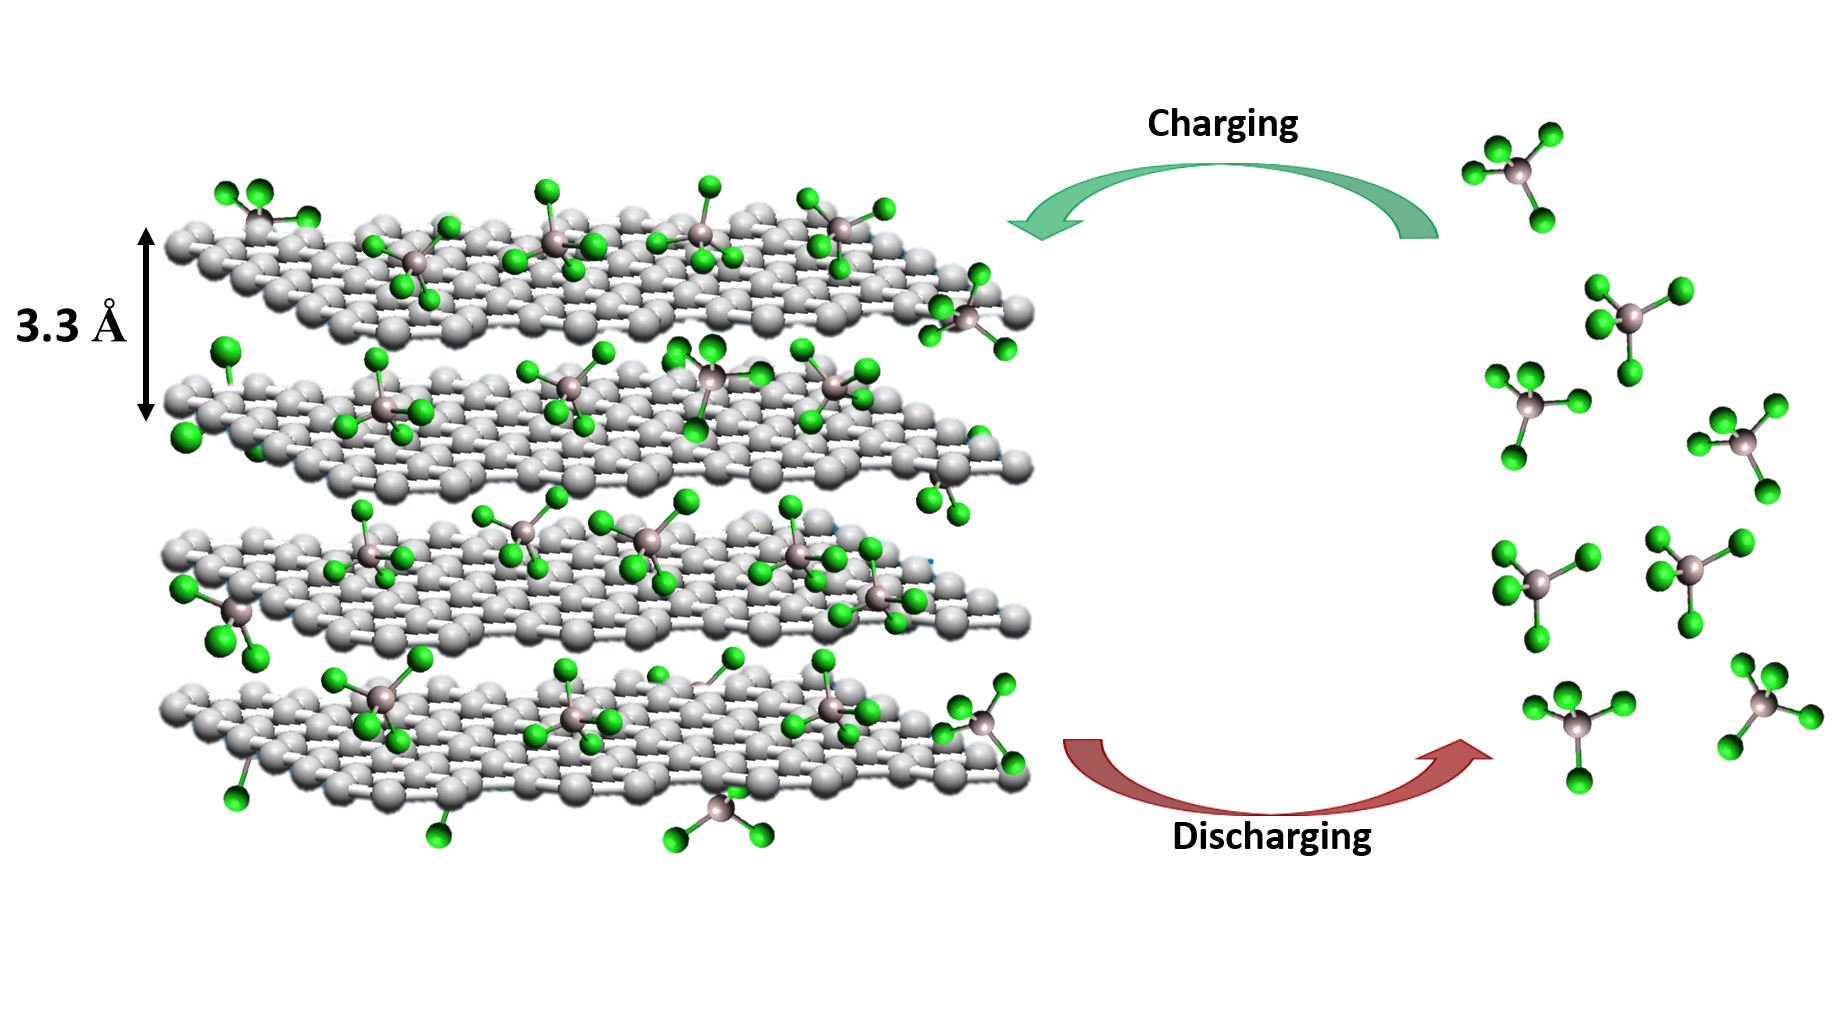
\includegraphics[width=\textwidth]{Figures/chap5fig/graphmech}
    \caption{Intercalation of \ce{AlCl4-} ions while cell charging and deintercalation during discharge in a Al/graphite cell. The interlayer distance between two graphite sheets is 3.3 \AA.}
  \label{Figures/chap5fig:graphmech}
\end{figure}
In this study, we compared four carbon-based materials with carbonised natural products. Super-P carbon has been used consistently as an additive to overcome any conductivity loss an active material suffers when a polymer binder such as PVDF, is added to it. Using it as an active material, we tried to find if Super-P contributes any capacity of its own to the battery's specific capacity. Activated carbon from natural products like rice or wood have been previously used in super-capacitors\cite{hussain_development_2019, frackowiak_carbon_2001}. Also known as 'hierarchical porous carbons', these structures contained pores of various sizes (mesopores and micropores), which enhanced the charge storage capacity by increasing the surface area of the electrodes . The pores absorb the charge carriers reversibly on their surface. Based on this hypothesis, we used activated carbon from human hair and hemp fibers as cathodes and got some interesting results. 
\section{Results and discussion}
\begin{table}[t]
\caption{Comparing average battery metrics of all carbon cathodes} \label{table1}
\begin{center}
\begin{tabular}{|lcccc|}
\hline
\textbf{Active material} & {\textbf{Size}} & \textbf{Specific capacity} & \textbf{Cell efficiency} & {\textbf{Cell voltage}}\\
 & (pore size) & (mAh g$^{-1}$) & $\%$ & (V)\\
\hline
Activated carbon & 5 ${\mu}$m & 102 & 97 & 1.9 \\
from human hair & & & & \\
Fullerene extract & 8.8 \AA & 78 & 85 & 1.7 \\
Hemp fibers & 2.3 $\mu$ m & 49 & 75 & 1.8 \\
Super-P & 300 \AA & 46 & 40 & 1.5 \\
\hline  % Please only put a hline at the end of the table
\end{tabular}
\end{center}
\end{table}
\begin{figure}[tbh!]
  \centering
  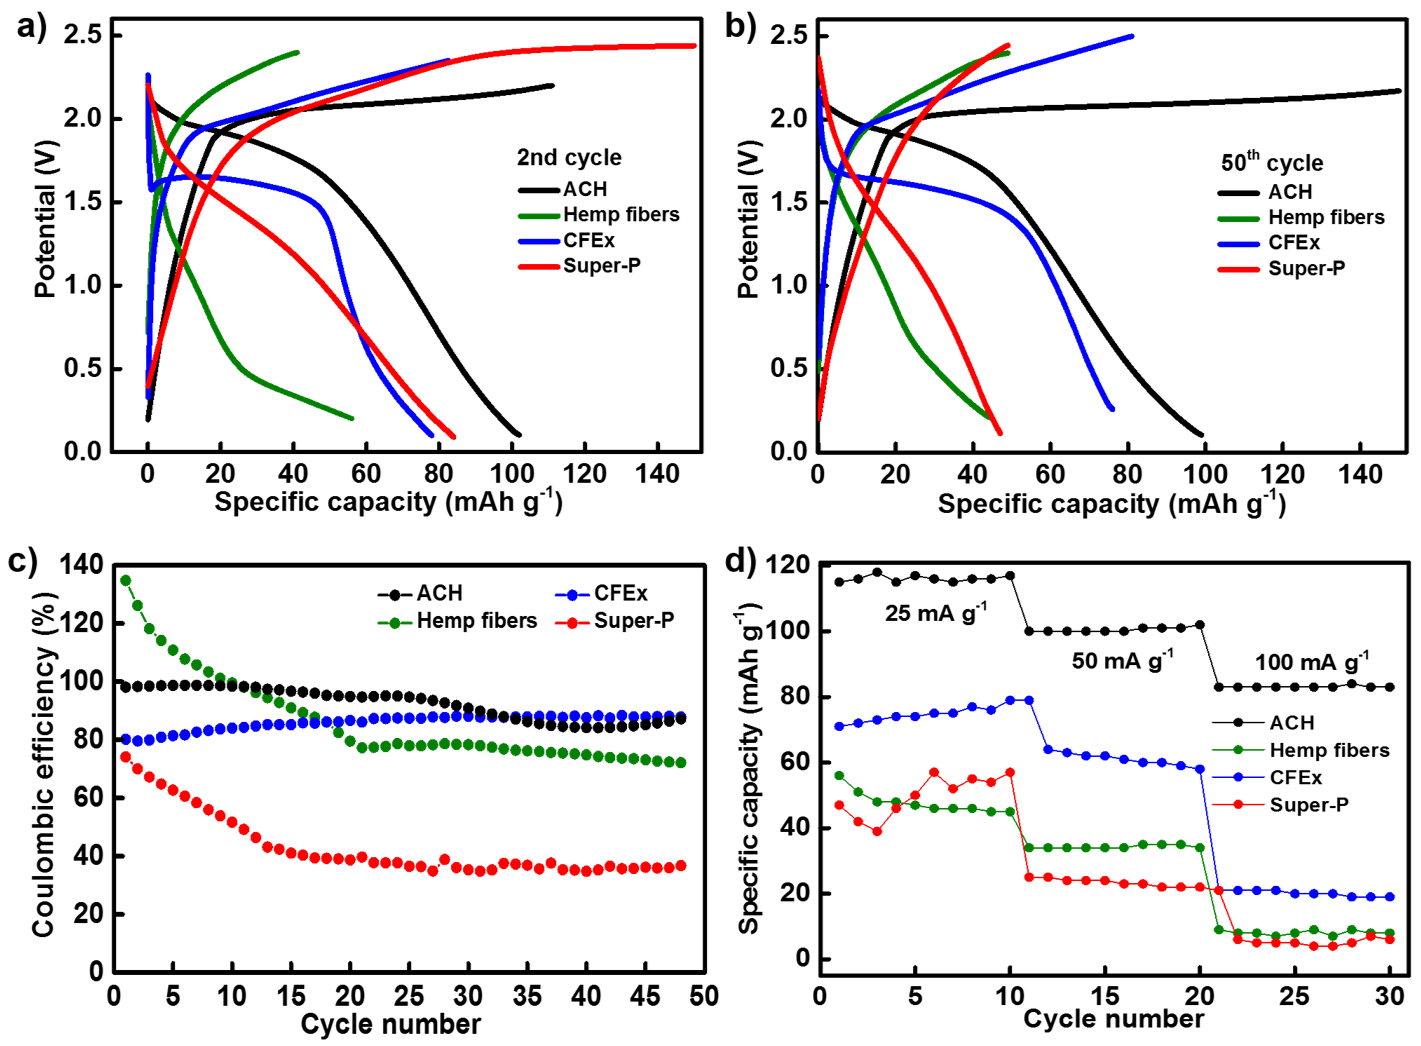
\includegraphics[width=\textwidth]{Figures/chap5fig/cdcall}
    \caption{Specific capacities in the a) 1$^{st}$ and b) 50$^{th}$ cycle of ACH, hemp fibers, CFEx and Super-P cathodes at a current rate of 50 mA g$^{-1}$. c) Cell efficiencies of cells at a current rate of 50 mAg$^{-1}$. d) Specific capacities of carbon cells at current rates of 25 mAg$^{-1}$, 50 mAg$^{-1}$ and 100 mAg$^{-1}$ in a two-electrode setup against Al$^{3+}$/Al. }
  \label{Figures/chap5fig:cdcall}
\end{figure}
Our battery system comprised of a cathode, 99\% pure aluminium foil as an anode and a room temperature ionic liquid (RTIL) acting as the electrolyte. ACH, hemp fibers and Super-P had an amorphous structure, however Raman spectra showed presence of a few graphitic planes. Any number of graphite-like layers would allow \ce{AlCl4-} ions to intercalate when the cell was charged. However, CFEx, a mixture of \ce{C60} and \ce{C70} fullerenes, had a crystalline lattice. Intercalation into the fullerene cage was not feasible because it needed a high amount of energy to break a C-C bond. We suggest that \ce{AlCl4-} anions seeped through the gaps present in between fullerenes without altering the molecular structure. Using a Neware BTS 3000 battery analyser, specific capacities of the cathodes were recorded at a constant current density of 50 mA g$^{-1}$ in Figure\ref{Figures/chap5fig:cdcall}a and b. Structural changes in the cathode before and after cycles was studied using their Raman spectra, XRD spectra and scanning electron microscopy (SEM) images.
ACH cells recorded the highest capacity at 102-mAh g$^{-1}$ and maintained it for 50 cycles. Coulombic efficiency was stable at ~95$\%$. Porous structure gave the material a high surface area that lead to an additional surface-based charge storage mechanism (observed in capacitors).Hemp fibers, due to their porous structure, observed a similar mechanism. Hemp cell showed a capacity of 56 mAh g$^{-1}$ in its first cycle, which decreased to 45 mAh g$^{-1}$ after 50 cycles. 
CFEx cell recorded its first discharge capacity at 79 mAh g$^{-1}$, which shifted to just 78 mAh g$^{-1}$. The cell maintained its coulombic efficiency at ~90$\%$. 
Specific capacity of the Super-P cell decreased considerably after repeated charge/ discharge cycles. With an initial capacity of 84 mAh g$^{-1}$, the value decreased to 47 mAh g$^{-1}$ with a low coulombic efficiency of $\sim$40$\%$. 
A low coulombic efficiency, which was also observed in the hemp cell, can be attributed to degradation of cathode structure, also known as cathode pulverisation. It seems due to continuous cycling, weak bonds existing between sections of the cathode broke and agglomerated into smaller chunks of C atoms. As a result, the number of surface pores decreased, which reduced the cell's capacity (Figure \ref{Figures/chap5fig:cdcall}c). 
Human hair has two components- cuticle and cortex. One way to make carbon porous is by treating it with an activating agent. Using activating agents especially alkali hydroxides improves the porosity and increases the surface area of material \cite{liu_hair-based_2017} .
In this work, sodium hydroxide (NaOH) was used as the activating agent, which breaks the weak interactions existing between the overlapping cells in the cortex. The reaction that takes place inside the matrix after adding NaOH is:
\begin{center}
    4NaOH + C $\longrightarrow$ 4Na + 4\ce{CO2} + 2\ce{H2O} \cite{qian_human_2013}
\end{center}

NaOH was reduced to Na, these atoms in turn expanded the carbon matrix. Oxidation of carbon formed \ce{CO2}, which created pores. An increase in temperature lead to Na activation, which was later removed from the matrix via channels created by \ce{CO2}. The channels created in this process provided path for \ce {AlCl4-} to intercalate inside the pores. The activating agent:carbon ratio and the calcinating temperature played an important role in determining the size of pores. The calcinating temperature used here was 750$^{\circ}$C. A schematic of ACH synthesis has been described in Figure \ref{Figures/chap5fig:achsyn}. Dong \textit{et al.} suggested that at higher temperatures (>900$^{\circ}$C) pores start to collapse resulting in graphitic sheets \cite{dong_commercial_2019}. 
Fibers obtained from Hemp (\textit{Cannabis Sativa L.}) have been used in several commercial items including paper, textiles, clothing, biodegradable plastics, paints, and bio-fuels. They have been used as reinforcements in composite materials and are capable of replacing glass fibers. Hemp fibers have a high moisture content which can be removed after high temperature treatment\cite{hussain_development_2019}. For creating activated carbon from these fibers, potassium hydroxide (KOH) was used as the activating agent. Since the samples were obtained from Carbon Valley\textsuperscript{\textregistered}, we are unable to report the precise calcinating temperature used. Unfortunately the structural domains appeared to have been damaged after this process. This phenomena negatively impacted its charge-storing capacity.  
Fullerenes have a fused-ring structure. The nucleus-to-nucleus diameter is 7.1\AA\ and van der Waals diameter is 11 \AA in a single crystal. Presence of $\pi$-electrons on its surface makes it a good electron acceptor. However, they are zero-dimensional materials, which means they cannot provide an efficient path for electron transport or a long-range conductivity\cite{loutfy_fullerene_2002, winkler_two-component_2007}. Electrochemical reduction of \ce{C60} to \ce{C60^{-3}} is highly reversible suggesting they are capable of giving reversible capacities. However, they are weak battery cathode materials owing to their solubility in electrolytes, especially in LIBs \cite{seger_prospects_1991}. To test their solubility in \ce{AlCl3}-EMImCl ionic liquid, 100 mg of CFEx was mixed in the electrolyte and stirred for 4 hours. For comparison, we mixed hemp fibers in another vial. The vials were left to stand for 24 hours in a \ce{N2}-filled glove box. A phase separation was observed with hemp fibers but not for CFEx indicating it dissolved in the electrolyte (Figure \ref{Figures/chap5fig:cfexsol}. It has been reported in Li-S batteries that poly-sulphides produced during charge-discharge were soluble in the electrolyte. It forms an insulating layer of \ce{Li2S} on the anode, which resulted in capacity fading \cite{sun_effect_2017}. However, reversible capacities obtained after 50 cycles suggested no such molecules were formed with \ce{AlCl3}/EmImCl electrolyte. 
 \begin{figure}[tbh!]
  \centering
  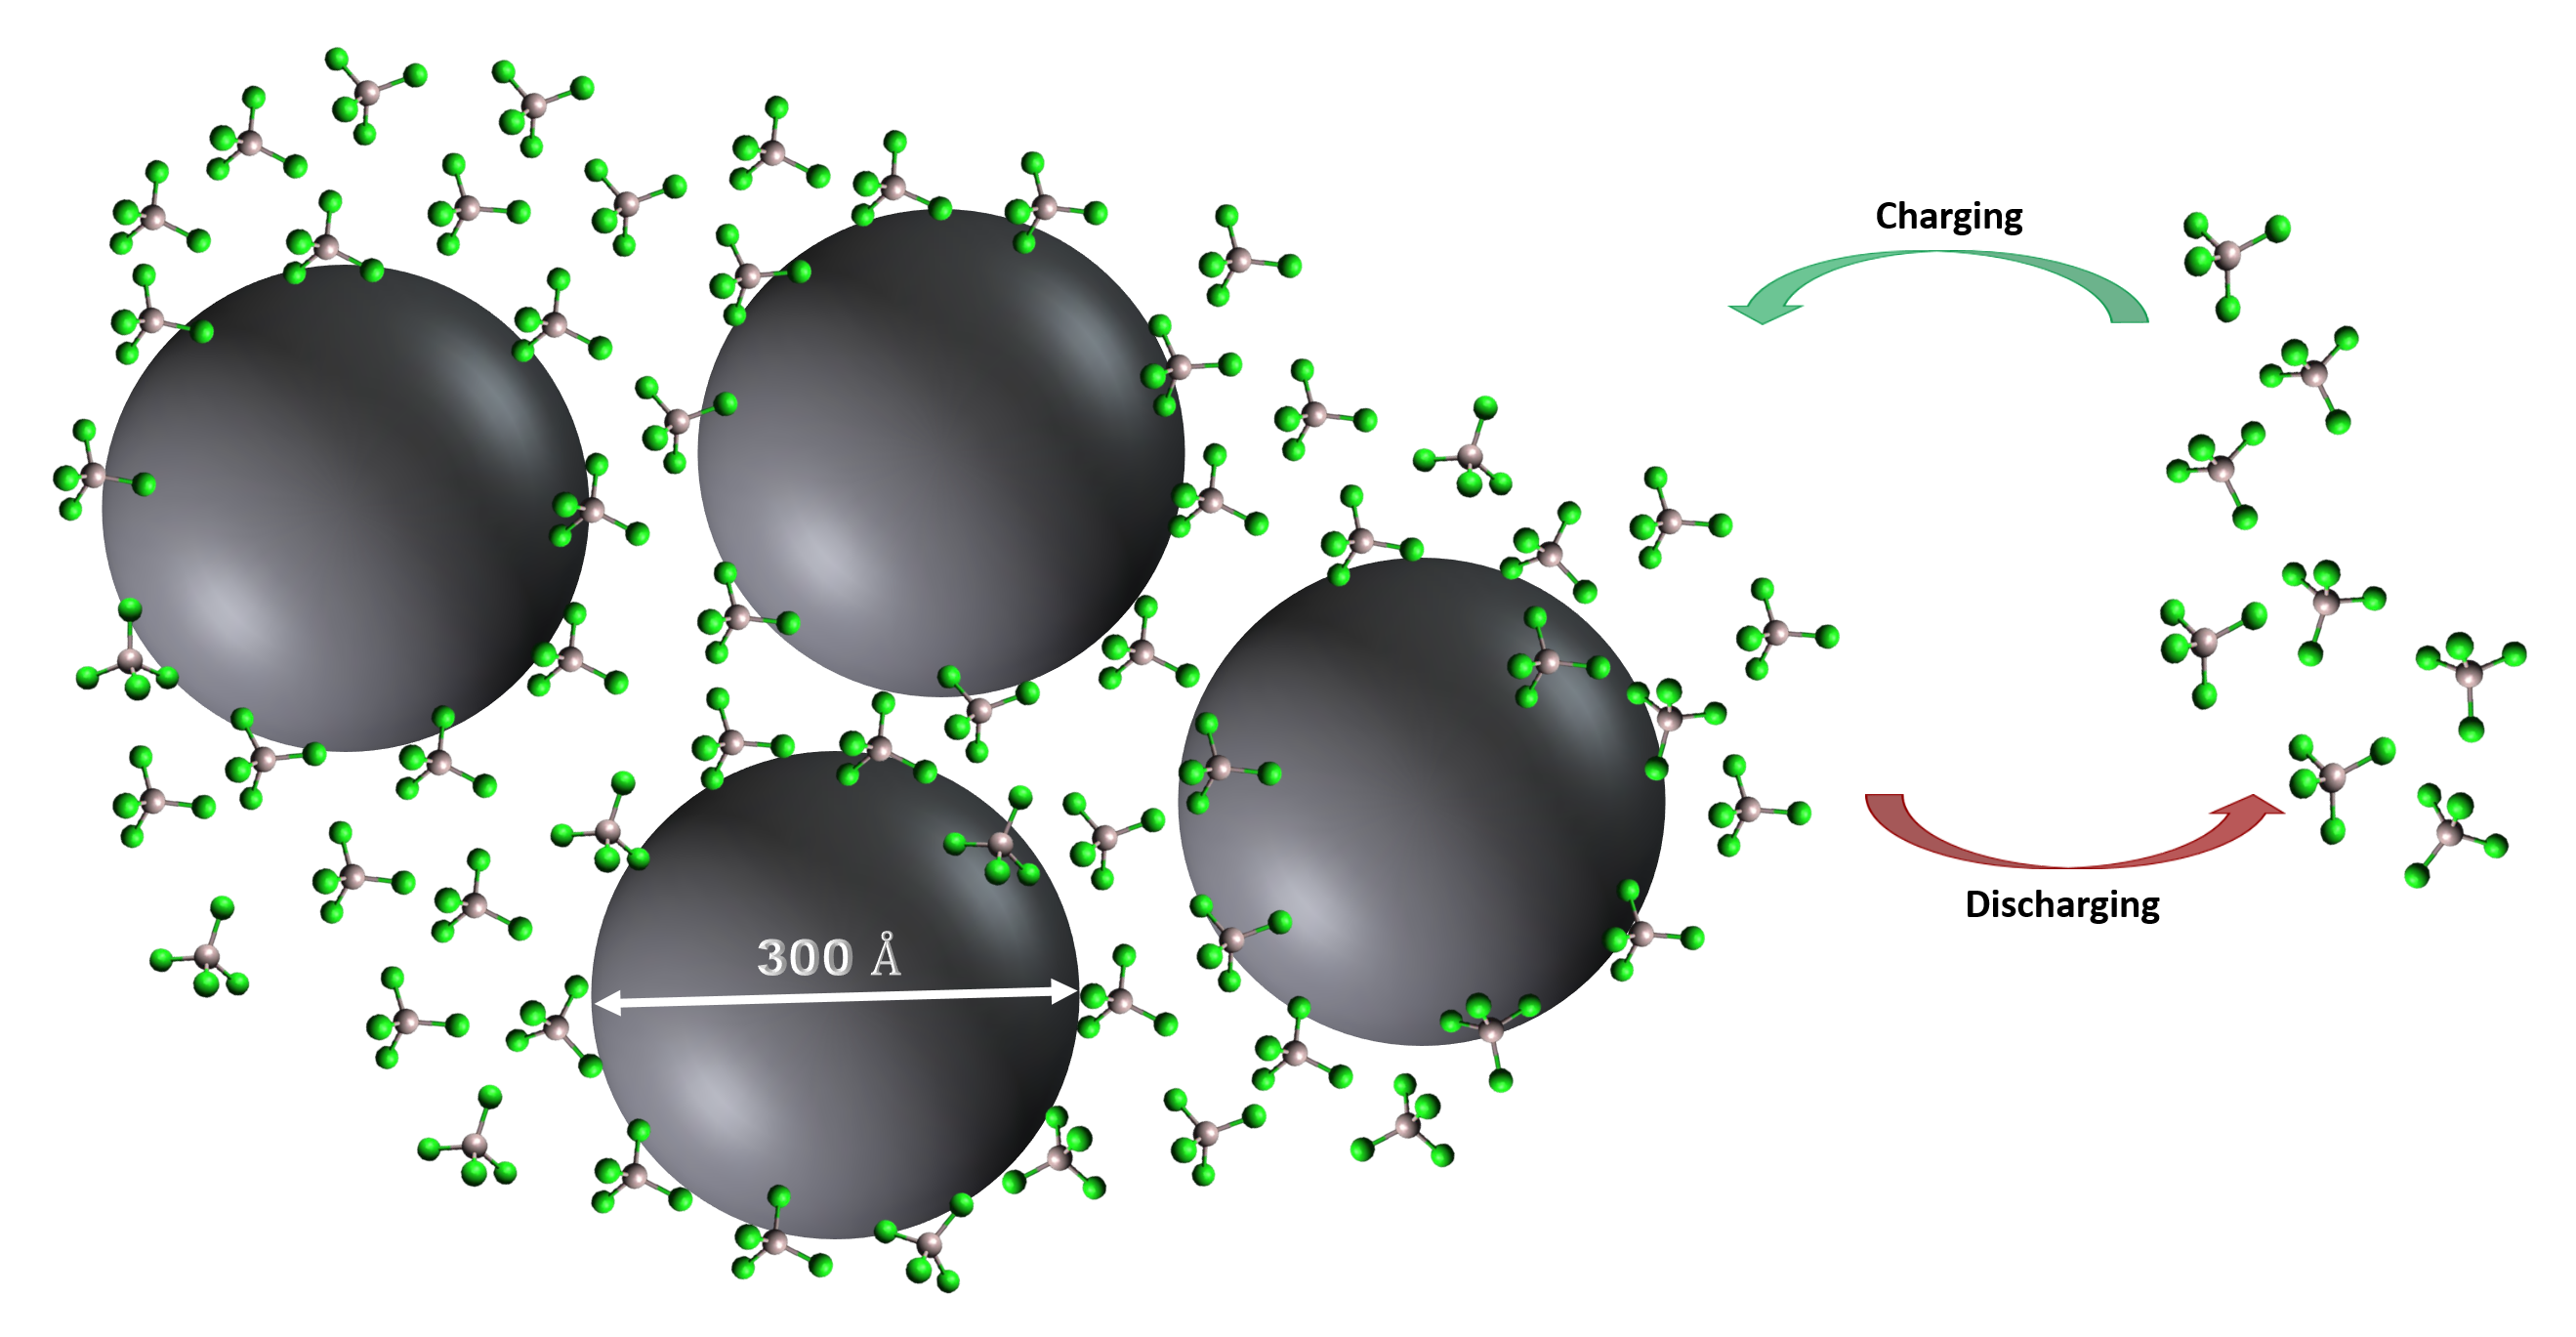
\includegraphics[width=\textwidth]{Figures/chap5fig/superpmech}
    \caption{Suggested mechanism for a \textbf{Al/Super-P} cell. Super-P has a very amorphous structure with a few graphite-like planes present in it. AlCl$_{4}^{-}$ ions intercalate into those layers and give the cell its capacity. However, cathode pulverisation results in capacity fading.}
  \label{Figures/chap5figs:superPmech}
\end{figure}
Pore size for Super-P ranges from ~30-50 nm \cite{younesi_analysis_2015}. It has the least graphitic structure when compared to ACH and hemp fibers. Loosely held structures, which disintegrated rapidly after every cycle resulted in reduced capacity and low coulombic efficiency values.


 \begin{figure}[tbh!]
  \centering
  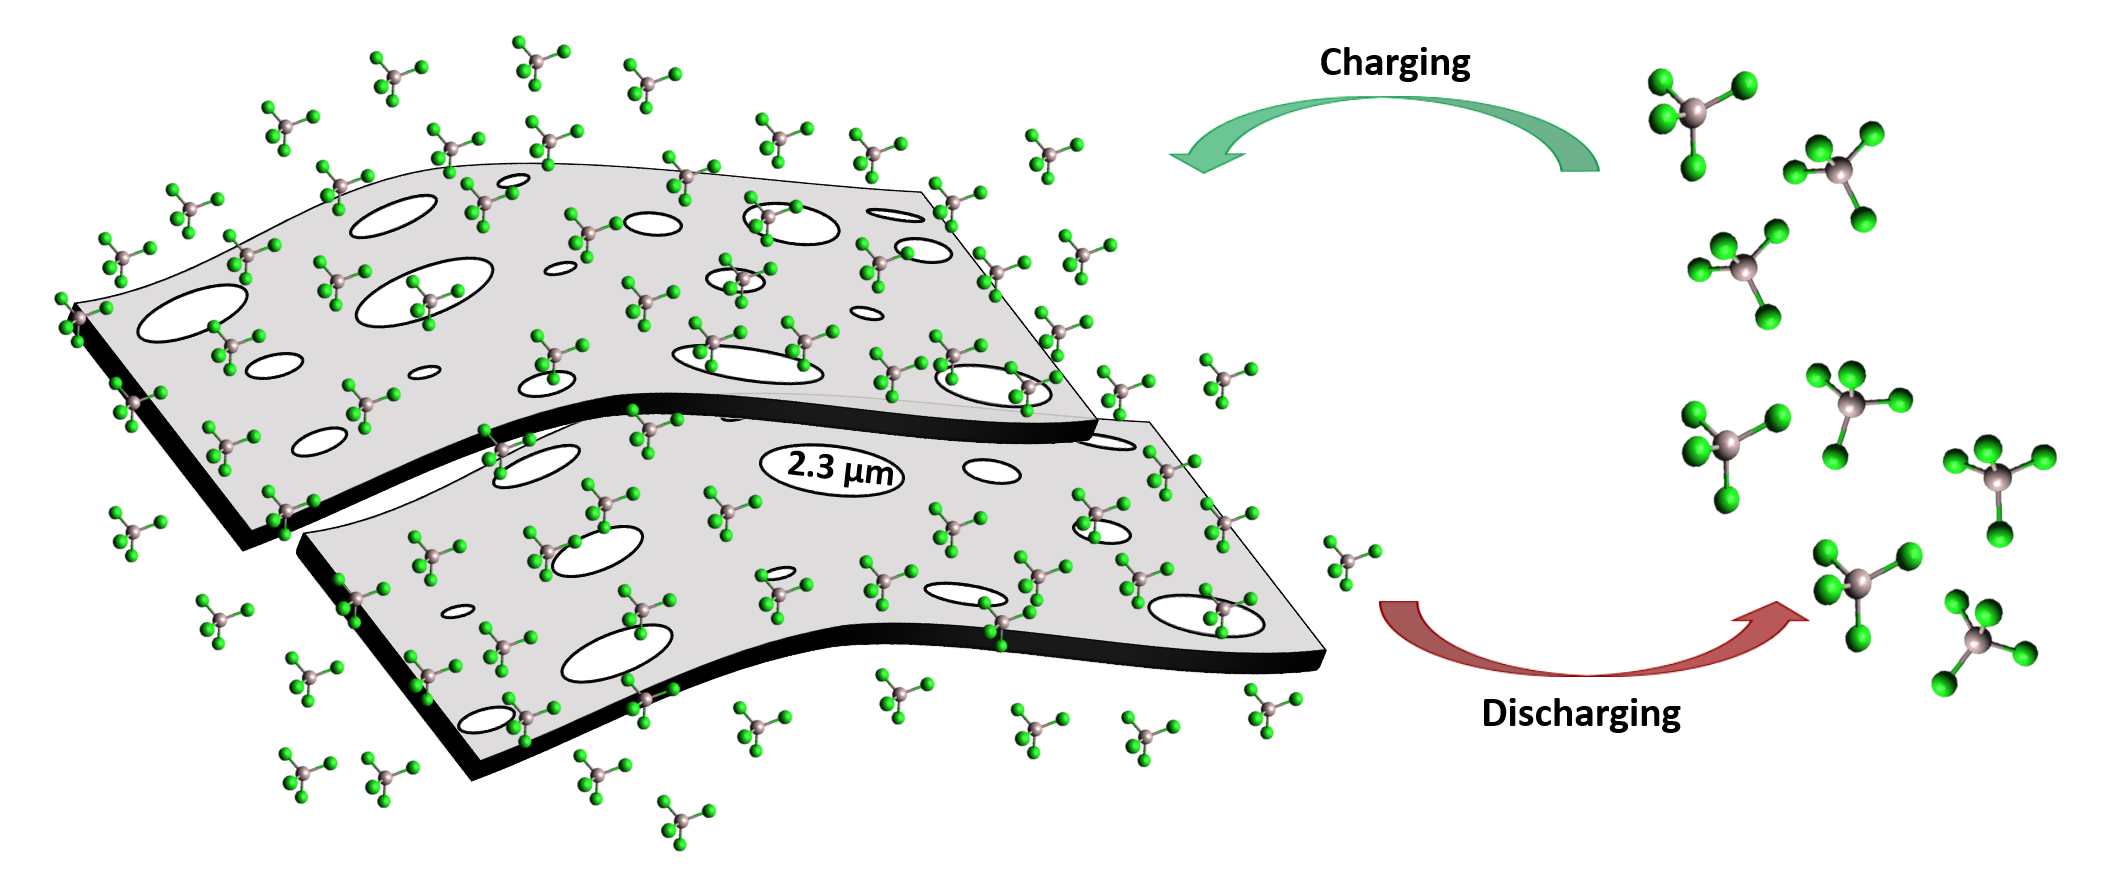
\includegraphics[width=\textwidth]{Figures/chap5fig/hempmech}
    \caption{Suggested mechanism for a \textbf{Al/hemp} cell. The fibers have a large pore size (2.0-2.5 $\mu$m) which allow the \ce{AlCl4-} to get absorbed on the cathode surface but agglomeration of carbon atoms after a few cycles reduces the active sites available for charge storage, which reduces cell's capacity after every cycle.}
  \label{Figures/chap5fig:hempmech}
\end{figure}
 \begin{figure}[tbh!]
  \centering
  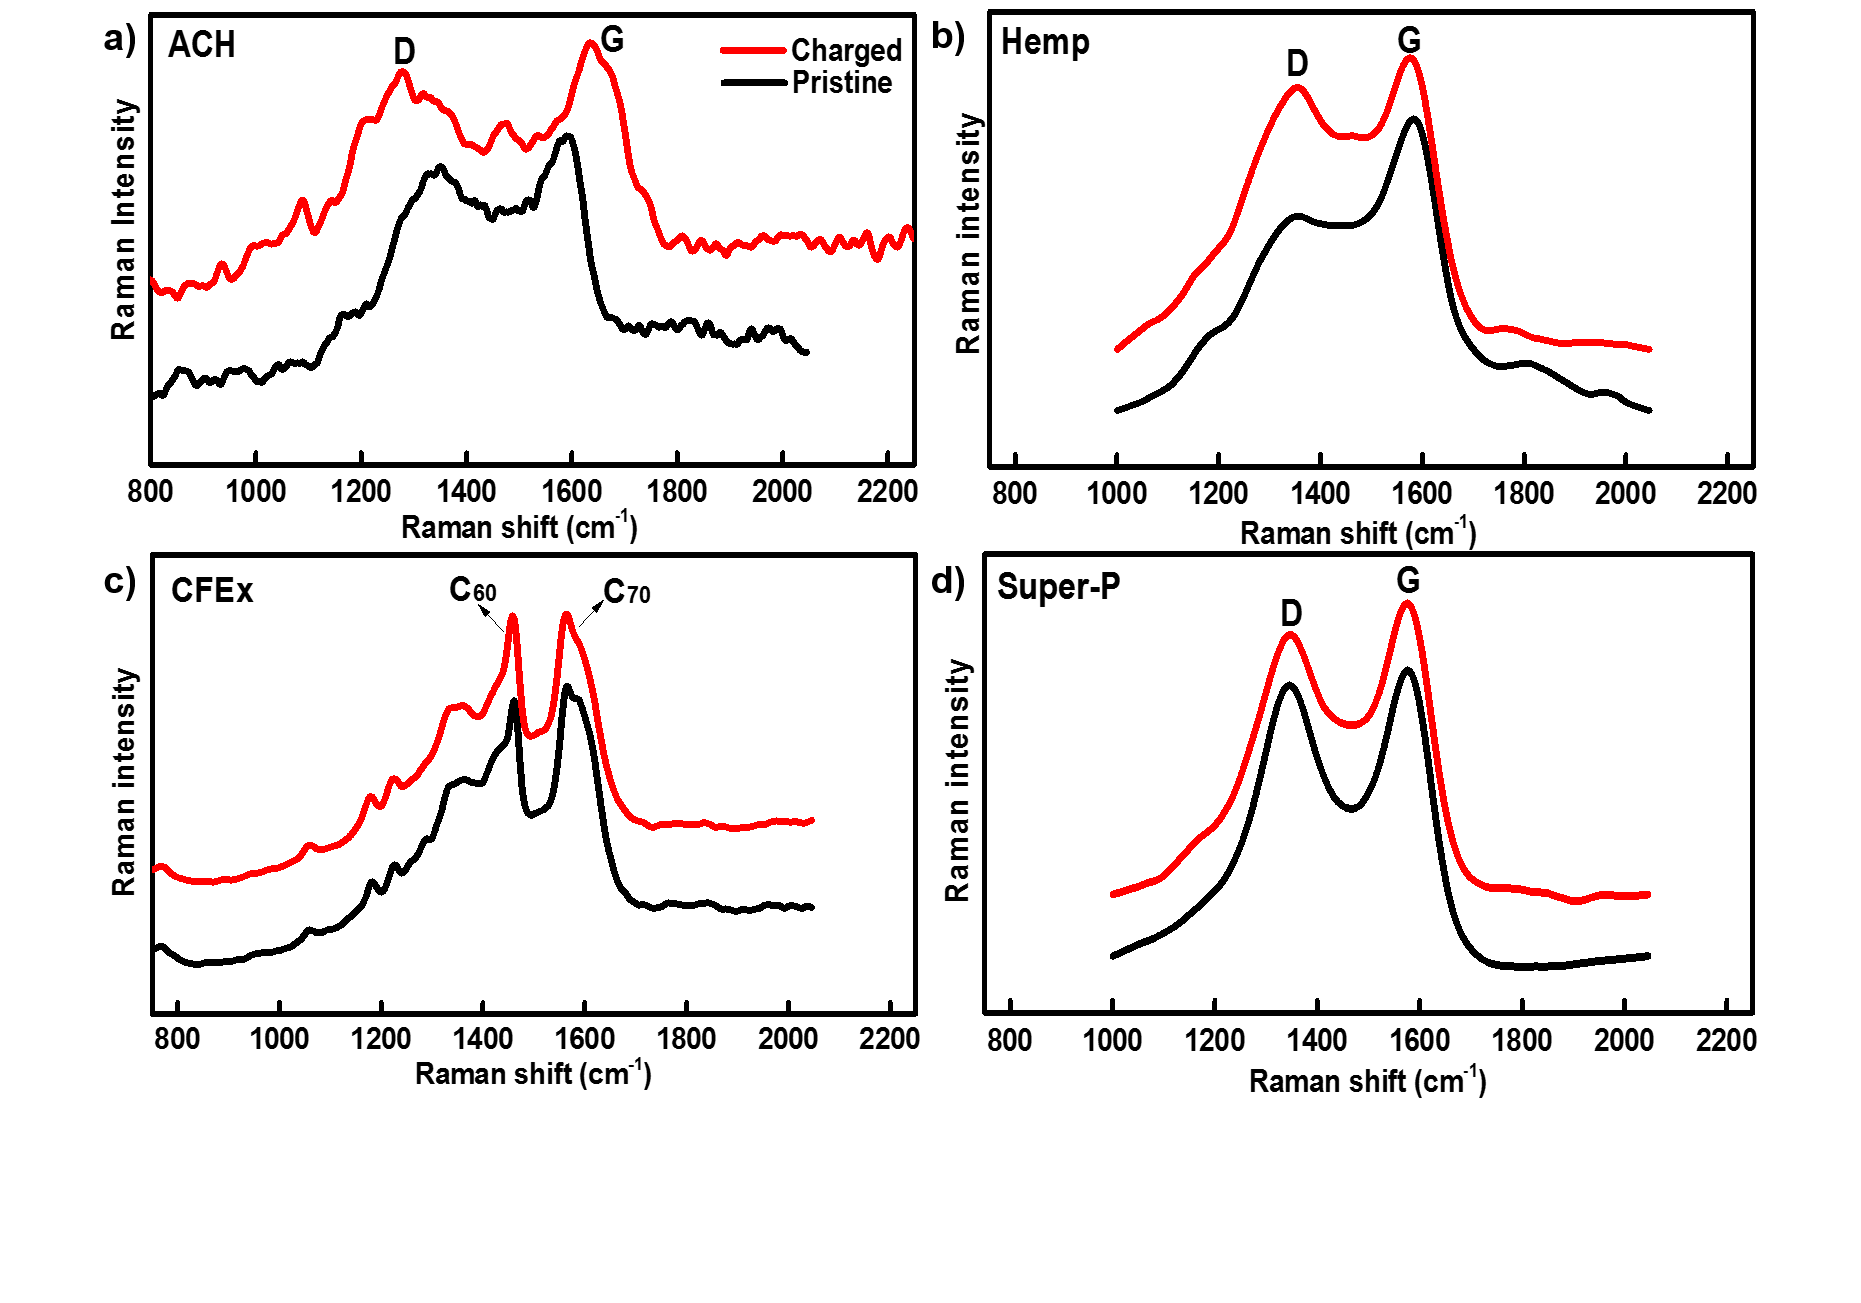
\includegraphics[width=\textwidth]{Figures/chap5fig/Raman}
    \caption{Raman spectra of pristine (in black) and charged (in red) a) CFEx , b) hemp fibers, c) ACH and d) Super-P cathodes indicating presence of both D and G-bands.}
  \label{Figures/chap5fig:Raman}
\end{figure}
Since it has been previously established that intercalation of \ce{AlCl$_{4}^{-}$} takes place in carbon materials during cell charge, we focused our analysis on the charged electrodes. Figure \ref{Figures/chap5fig:Raman} illustrates Raman spectra of the tested cathodes. Pristine ACH, hemp fibers and Super-P had a significant D-band indicating a distorted lattice. Increased intensity of D band can be seen in charged electrodes at ~1300 cm$^{-1}$ (ACH), 1329.7 cm$^{-1}$ (hemp fibers), and 1352.0 cm$^{-1}$ (Super-P) indicating an increase in the lattice defects and deformities. Hemp fibers and ACH observed an increased FWHM (full width at half maximum) of both D and G bands indicating a loss in symmetry. Intercalation of ions or surface adsorption of anions onto the porous carbon cathode, would alter the ordered structure on the surface. We suggest capacitive intercalation mechanism as well as a redox pseudocapacitance where \ce{AlCl4-} ions electrochemically adsorb onto the surface \cite{brezesinski_ordered_2010}. 
The main feature in a fullerene Raman spectrum was a sharp line observed at 1460 cm$^{-1}$, which is known as the 'pentagonal pinch mode'. \ce{C60} is composed of \ce{sp2} bonded carbon atoms. Sharpness of the band indicates a uniform nature of the bonds. However, the spectrum of \ce{C70} has multiple bands. Reduction in its molecular symmetry increases the number of active Raman bands \cite{}. Pristine CFEx electrode observed characteristic peaks of both \ce{C60} and \ce{C70} at 1459.3 cm$^{-1}$ and 1564 cm$^{-1}$ respectively in Figure \ref{Figures/chap5fig:Raman}c. An interesting observation was that pristine and charged CFEx electrodes had a similar-looking spectra after cycling. Since Raman spectroscopy is sensitive to very minute differences in molecular morphology, the results suggested that the structure remained intact. Another interesting observation was made in charged ACH electrode (Figure \ref{Figures/chap5fig:Raman}a). A new peak appeared at 1466 cm$^{-1}$. A similar band splitting was observed by Wang \textit{et al} \cite{wang_kish_2017} while charging natural graphite and \ce{AlCl4-} ions intercalated into the cathode layers. This peak appeared due to vibration of carbon atoms in a plane adjacent to intercalant layer planes. We observed no such effect was observed for any other cathode. Since the Al/ACH cell maintained a highly reversible capacity of 102 mAhg$^{-1}$ after 50 cycles, we assume ACH underwent a similar mechanism, where \ce{AlCl4-} ions intercalate into the cathode during charge. ACH has a high surface area and an inter-connected mesoporosity. The layered domains present in it enable insertion of \ce{AlCl4-}, while a few anions get electrochemically adsorbed onto the surface through a charge-transfer process resulting in a redox pseudo-capacitance. All these processes seem to take place at the same time without changing the reaction kinetics. Additionally, presence of both an amorphous and crystalline structure in this material increases the charge-storage capacity of the material \cite{brezesinski_ordered_2010}. This might be the reason why ACH shows a remarkable reversibility. Schematic of a possible mechanism is shown in Figure \ref{Figures/chap5fig:achmech}. Hemp fibers and Super-P had lattice deformities to begin with, which were enhanced after the cell underwent the preliminary galvanostatic cycles. This decreased capacity after every cycle. 
\begin{figure}[tbh!]
  \centering
  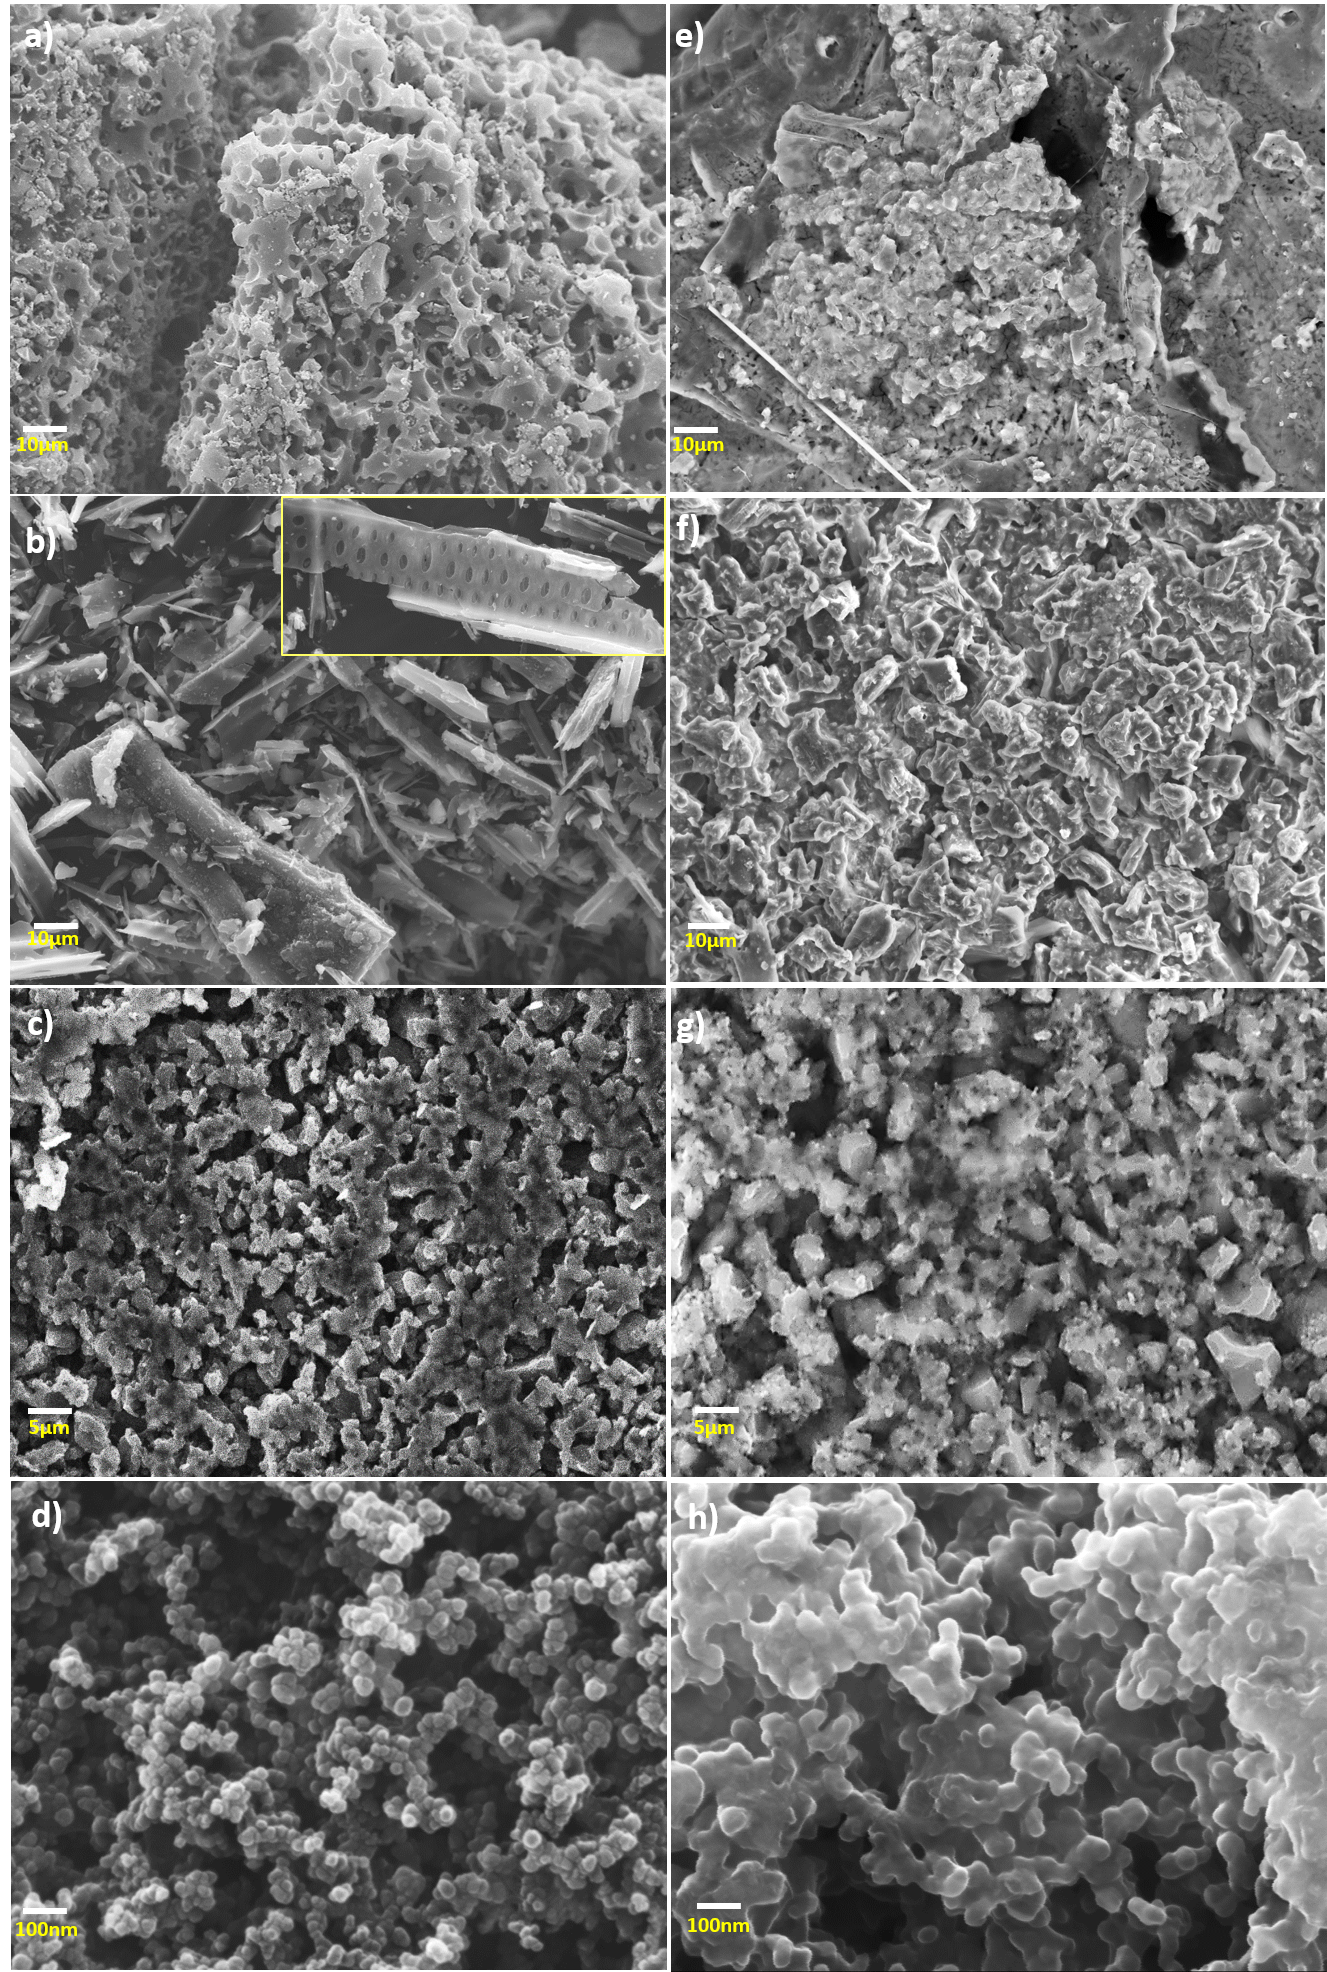
\includegraphics[width=0.6\textwidth]{Figures/chap5fig/SEM}
    \caption{Scanning electron microscopy images comparing pristine a) ACH, b) hemp fibers, c) CFEx and d) Super-P; and charged e)ACH, f) hemp fibers, g) CFEx and h) Super-P electrodes. Hemp fibers and Super-P undergo prominent changes after charge/discharge cycles (visible agglomeration of carbon atoms).}
  \label{Figures/chap5fig:SEM}
\end{figure}
Above results seem to be in good agreement with SEM images in Figure 9, where we compared pristine (Figure \ref{Figures/chap5fig:SEM}a, b, c and d) and charged electrodes (\ref{Figures/chap5fig:SEM}e,f,g and h). ACH and hemp fibres have a porous structure (Figure \ref{Figures/chap5fig:SEM}a and 9b), which looked visibly degraded after cycles (Figure \ref{Figures/chap5fig:SEM}e and f). Agglomeration of carbon atoms increases the edge defects in a material. This explains the high intensity of D-bands of these cathodes, Figure \ref{Figures/chap5fig:Raman}. Surface morphology of CFEx (Figure \ref{Figures/chap5fig:SEM}c did not change a lot after charge (Figure \ref{Figures/chap5fig:SEM}g), similar to our observations in its Raman spectra. 
\begin{figure}[tbh!]
  \centering
  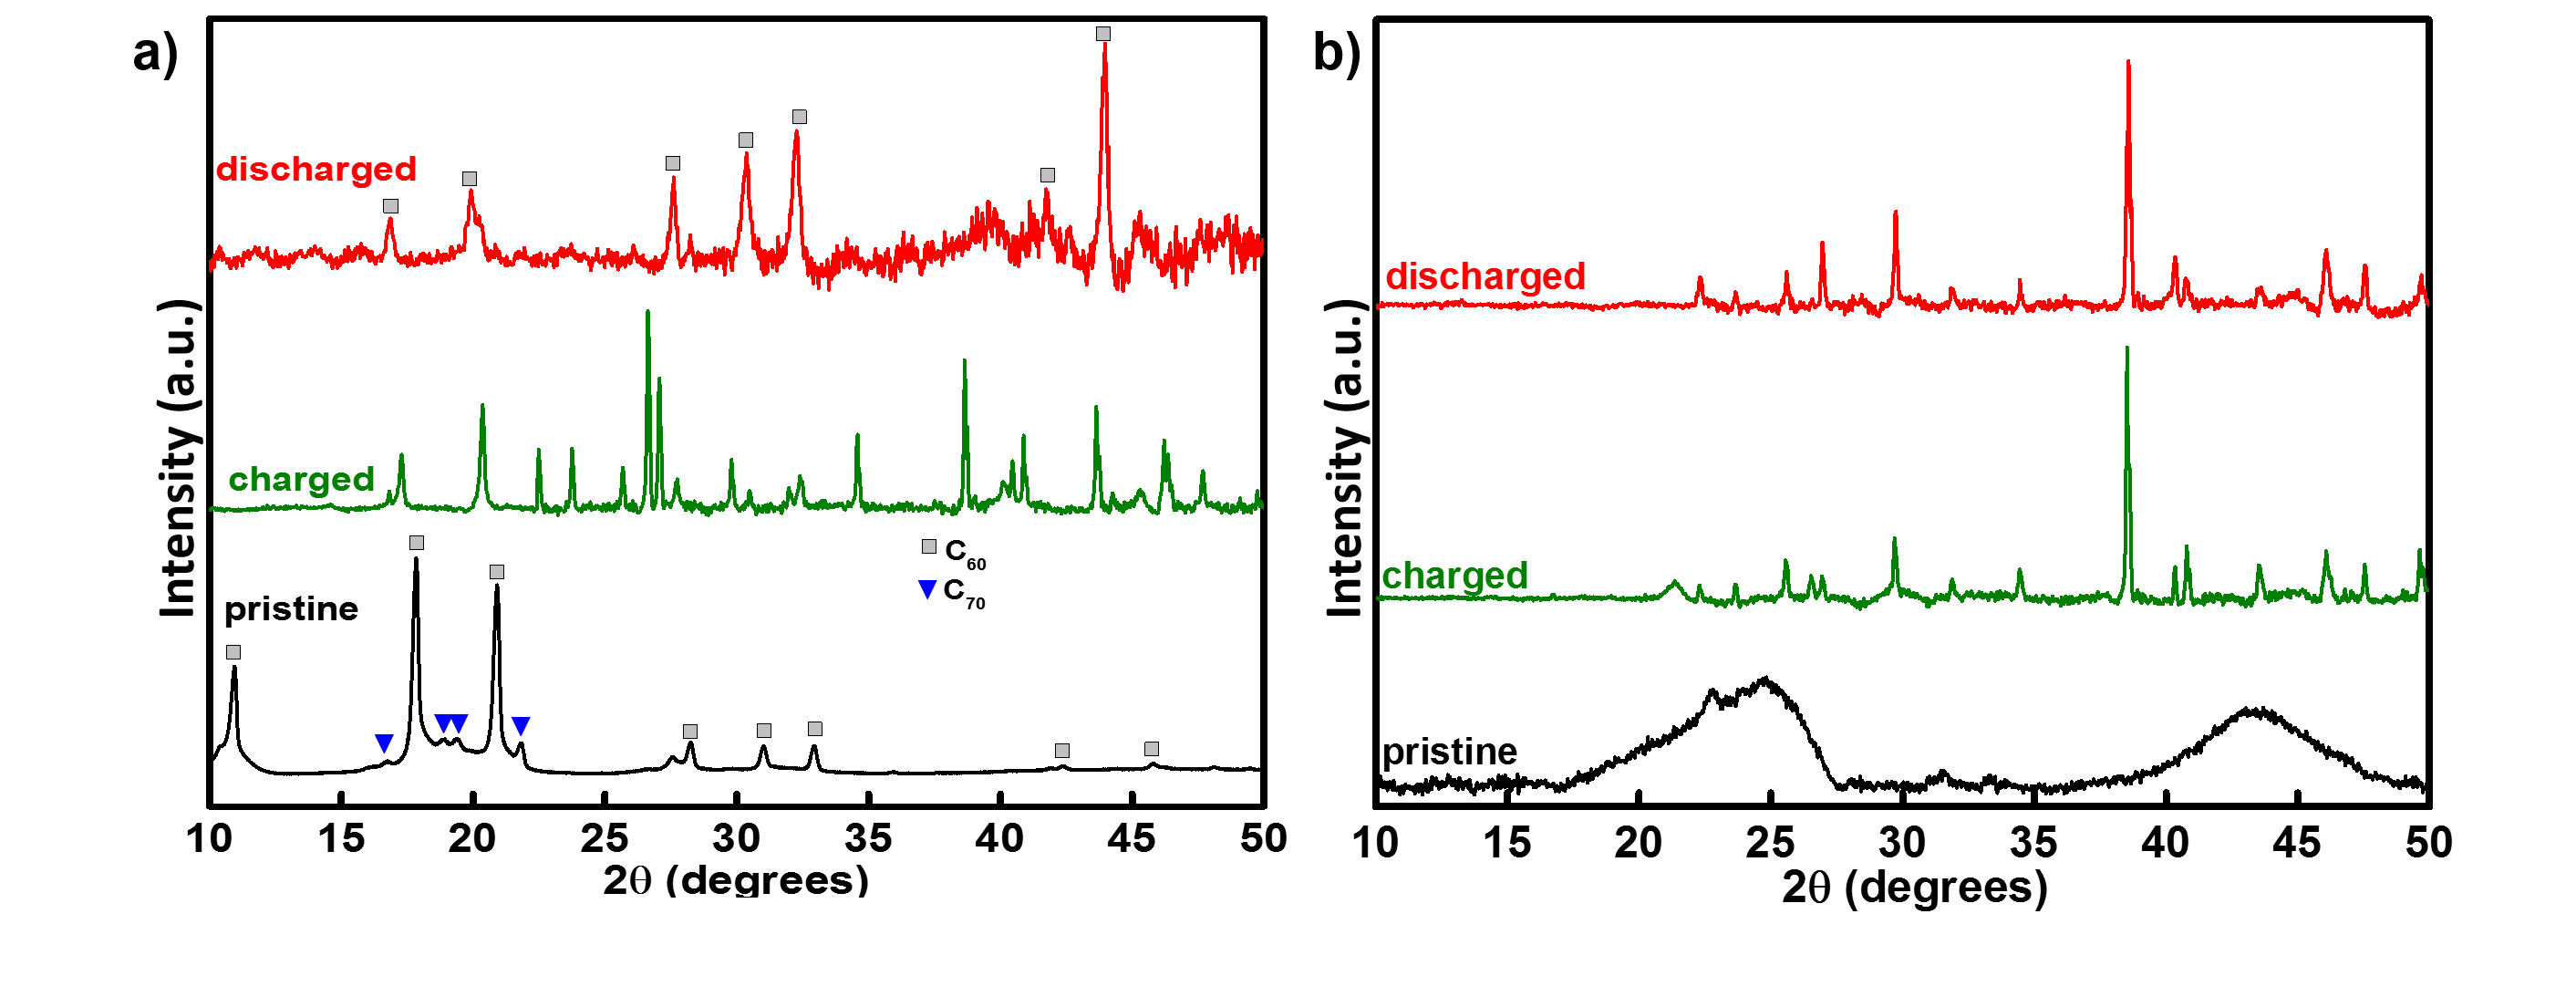
\includegraphics[width=\textwidth]{Figures/chap5fig/xrd}
    \caption{XRD spectra comparing a pristine (black), charged (green) and discharged (red) a) CFEx and b)ACH cathode to study changes in their lattice after 50 galvanostatic cycles in a two-electrode setup against \ce{Al$^{3+}$/Al} with characteristic peaks marked for \ce{C60} (in grey) and \ce{C70} (in blue).}
  \label{Figures/chap5fig:xrd}
\end{figure}
To confirm the reversible electrochemical processes taking place in CFEx and ACH, we examined their XRD spectra (pristine, charged and discharged) in Figure \ref{Figures/chap5fig:xrd}a and b respectively. Pristine cathode recorded the characteristic peaks of both \ce{C60} and \ce{C70}, which reappeared after discharge suggesting a reversible process. However, charged electrode observed new diffraction peaks which can be attributed to lattice deformities taking place at the electrode/electrolyte interface. We calculated the unit cell lattice parameters for both pristine and charged cathode for a \ce{C60} molecule. The unit cell had a tetragonal crystal system with space group of P42/mmc and a space group number 131 (ICDD: 04-013-1339 for \ce{C60}). Lattice parameter 'a' and 'b' for the charged electrode changed from 9.06 \AA to 9.57 \AA . Lattice parameter 'c' changed from 15.03 \AA to 15.65 \AA, in Figure \ref{Figures/chap5fig:cfexcrys}a and b. Lattice parameters for discharged cathode were closer to pristine values. The changes in the fullerene structure suggested a reversible intercalation process taking place, where the unit cells shifted from their original location during charge and returned back after discharge. A possible site for \ce{AlCl4-} intercalation is depicted in Figure \ref{Figures/chap5fig:cfexcrys}c. XRD spectra for ACH electrodes was inconclusive (Figure \ref{Figures/chap5fig:xrd}b). Pristine cathode observed very broad peaks suggesting the extreme amorphous nature of the material. However, the material seemed to have a more ordered structure after the galvanostatic cycles. It seems that surface-based charge-storage was more dominant than the intercalation process. This is why presence of crystallinity in the active material does not limit the surface-based charge storage and therefore, the capacity remains same \cite{kim_synthesis_2006, jow_factors_2018}. 
 \begin{figure}[tbh!]
  \centering
  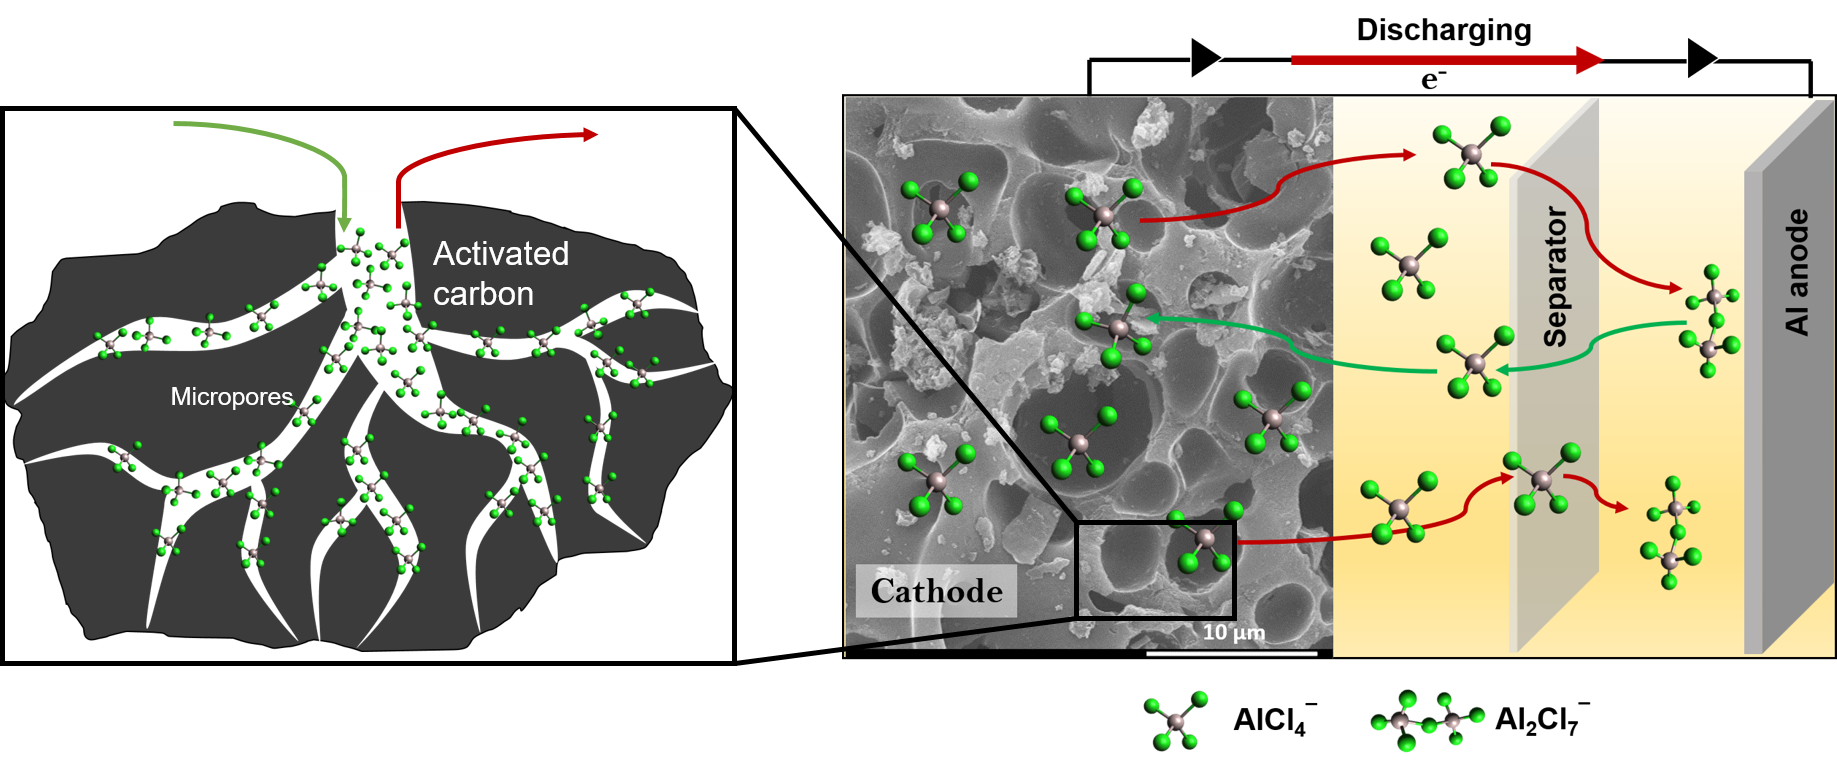
\includegraphics[width=\textwidth]{Figures/chap5fig/achmech}
    \caption{Suggested mechanism for a \textbf{Al/ACH} cell. ACH has a porous structure which allows \ce{AlCl4-} ions to get absorbed as well as reversibly intercalate into the graphitic planes, giving additional capacity to the cell.}
  \label{Figures/chap5fig:achmech}
\end{figure}

\begin{figure}[tbh!]
  \centering
  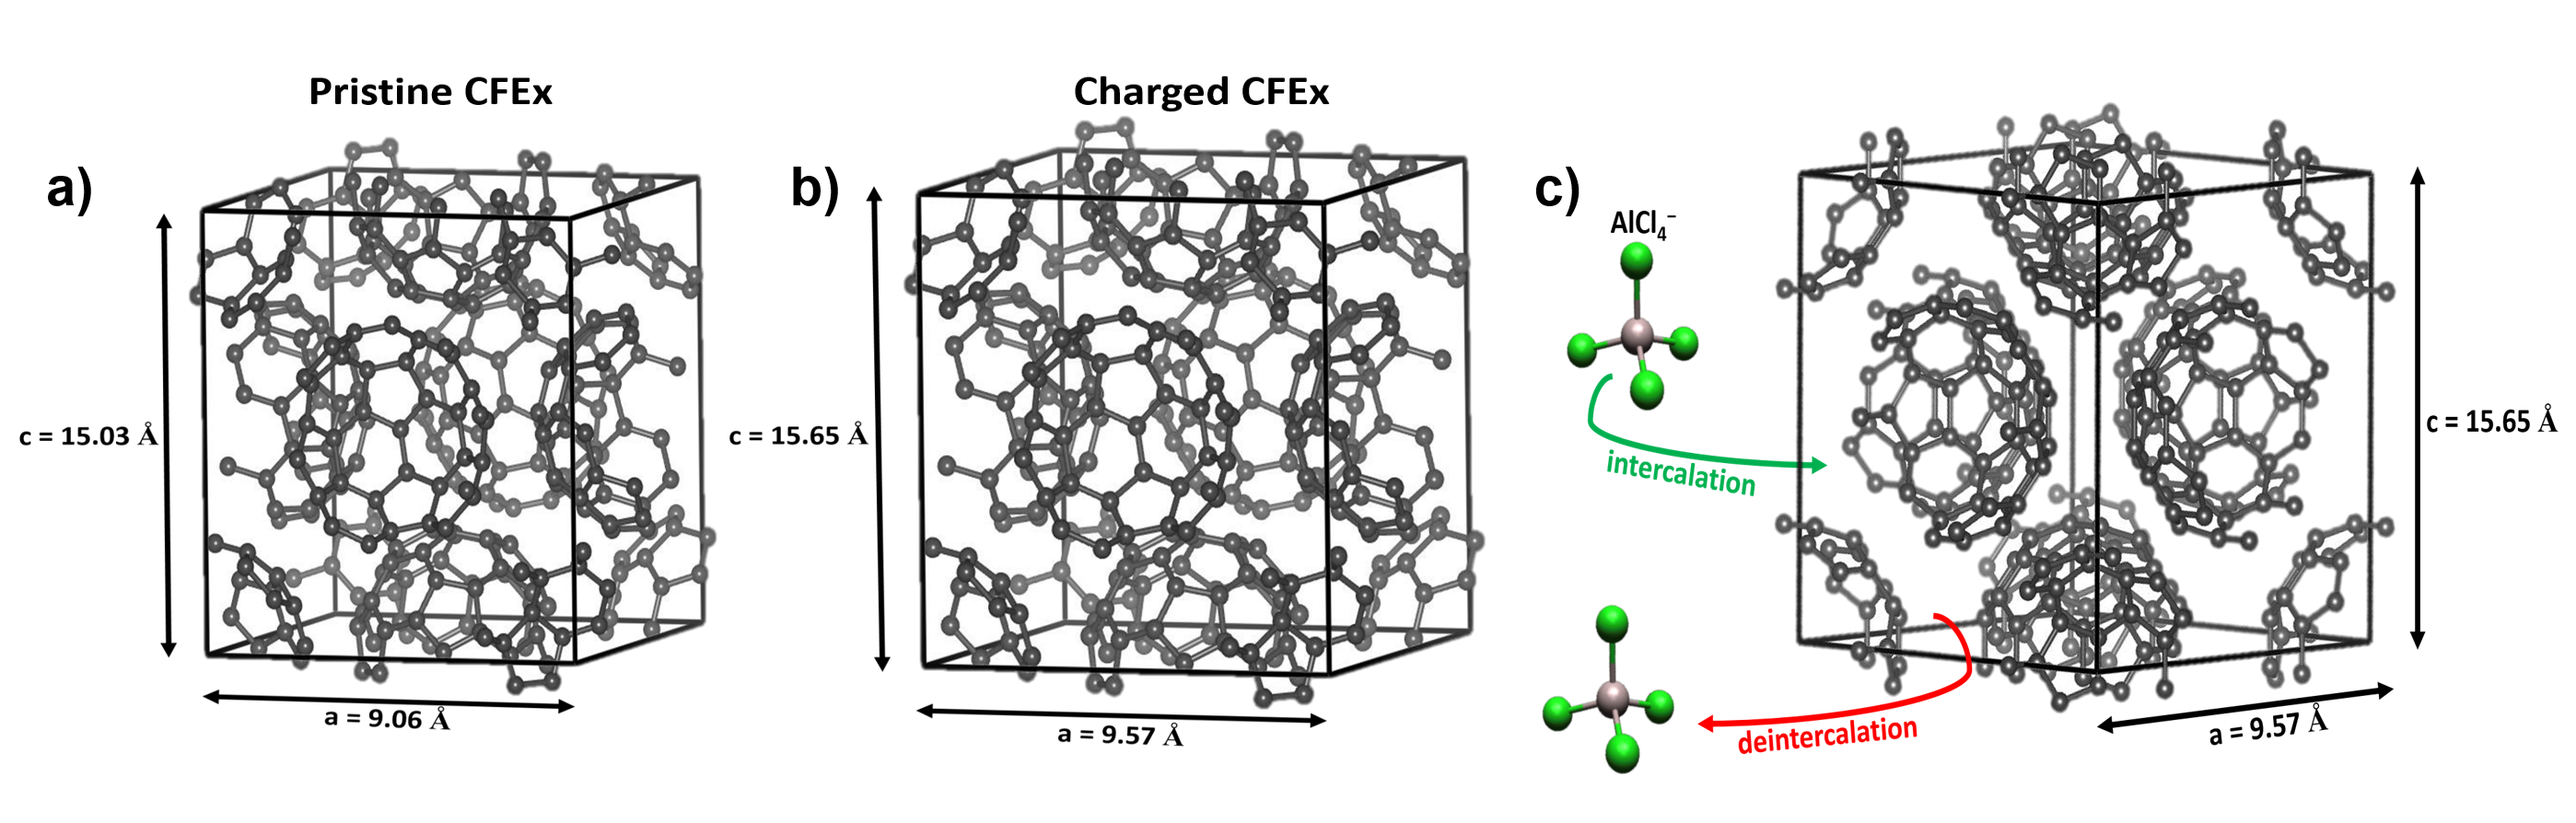
\includegraphics[width=\textwidth]{Figures/chap5fig/cfexcrys}
    \caption{Changes in the lattice parameters of a \ce{C60} unit cell. a) Pristine \ce{C60}unit cell, b) charged \ce{C60}unit cell with increased parameters suggesting a uniform shift in the lattice after charge/discharge. c) Expected intercalation sites of \ce{AlCl4-} ions in the unit cell.}
  \label{Figures/chap5fig:cfexcrys}
\end{figure}
%Charged Super-P and hemp fiber electrodes underwent degradation and appeared clumped together resulting in capacity decay. This was visible from their electrochemical results where a rapid decrease in capacity and cell efficiency was noted. 
%XPS analysis results... C 1s 
\begin{figure}[tbh!]
  \centering
  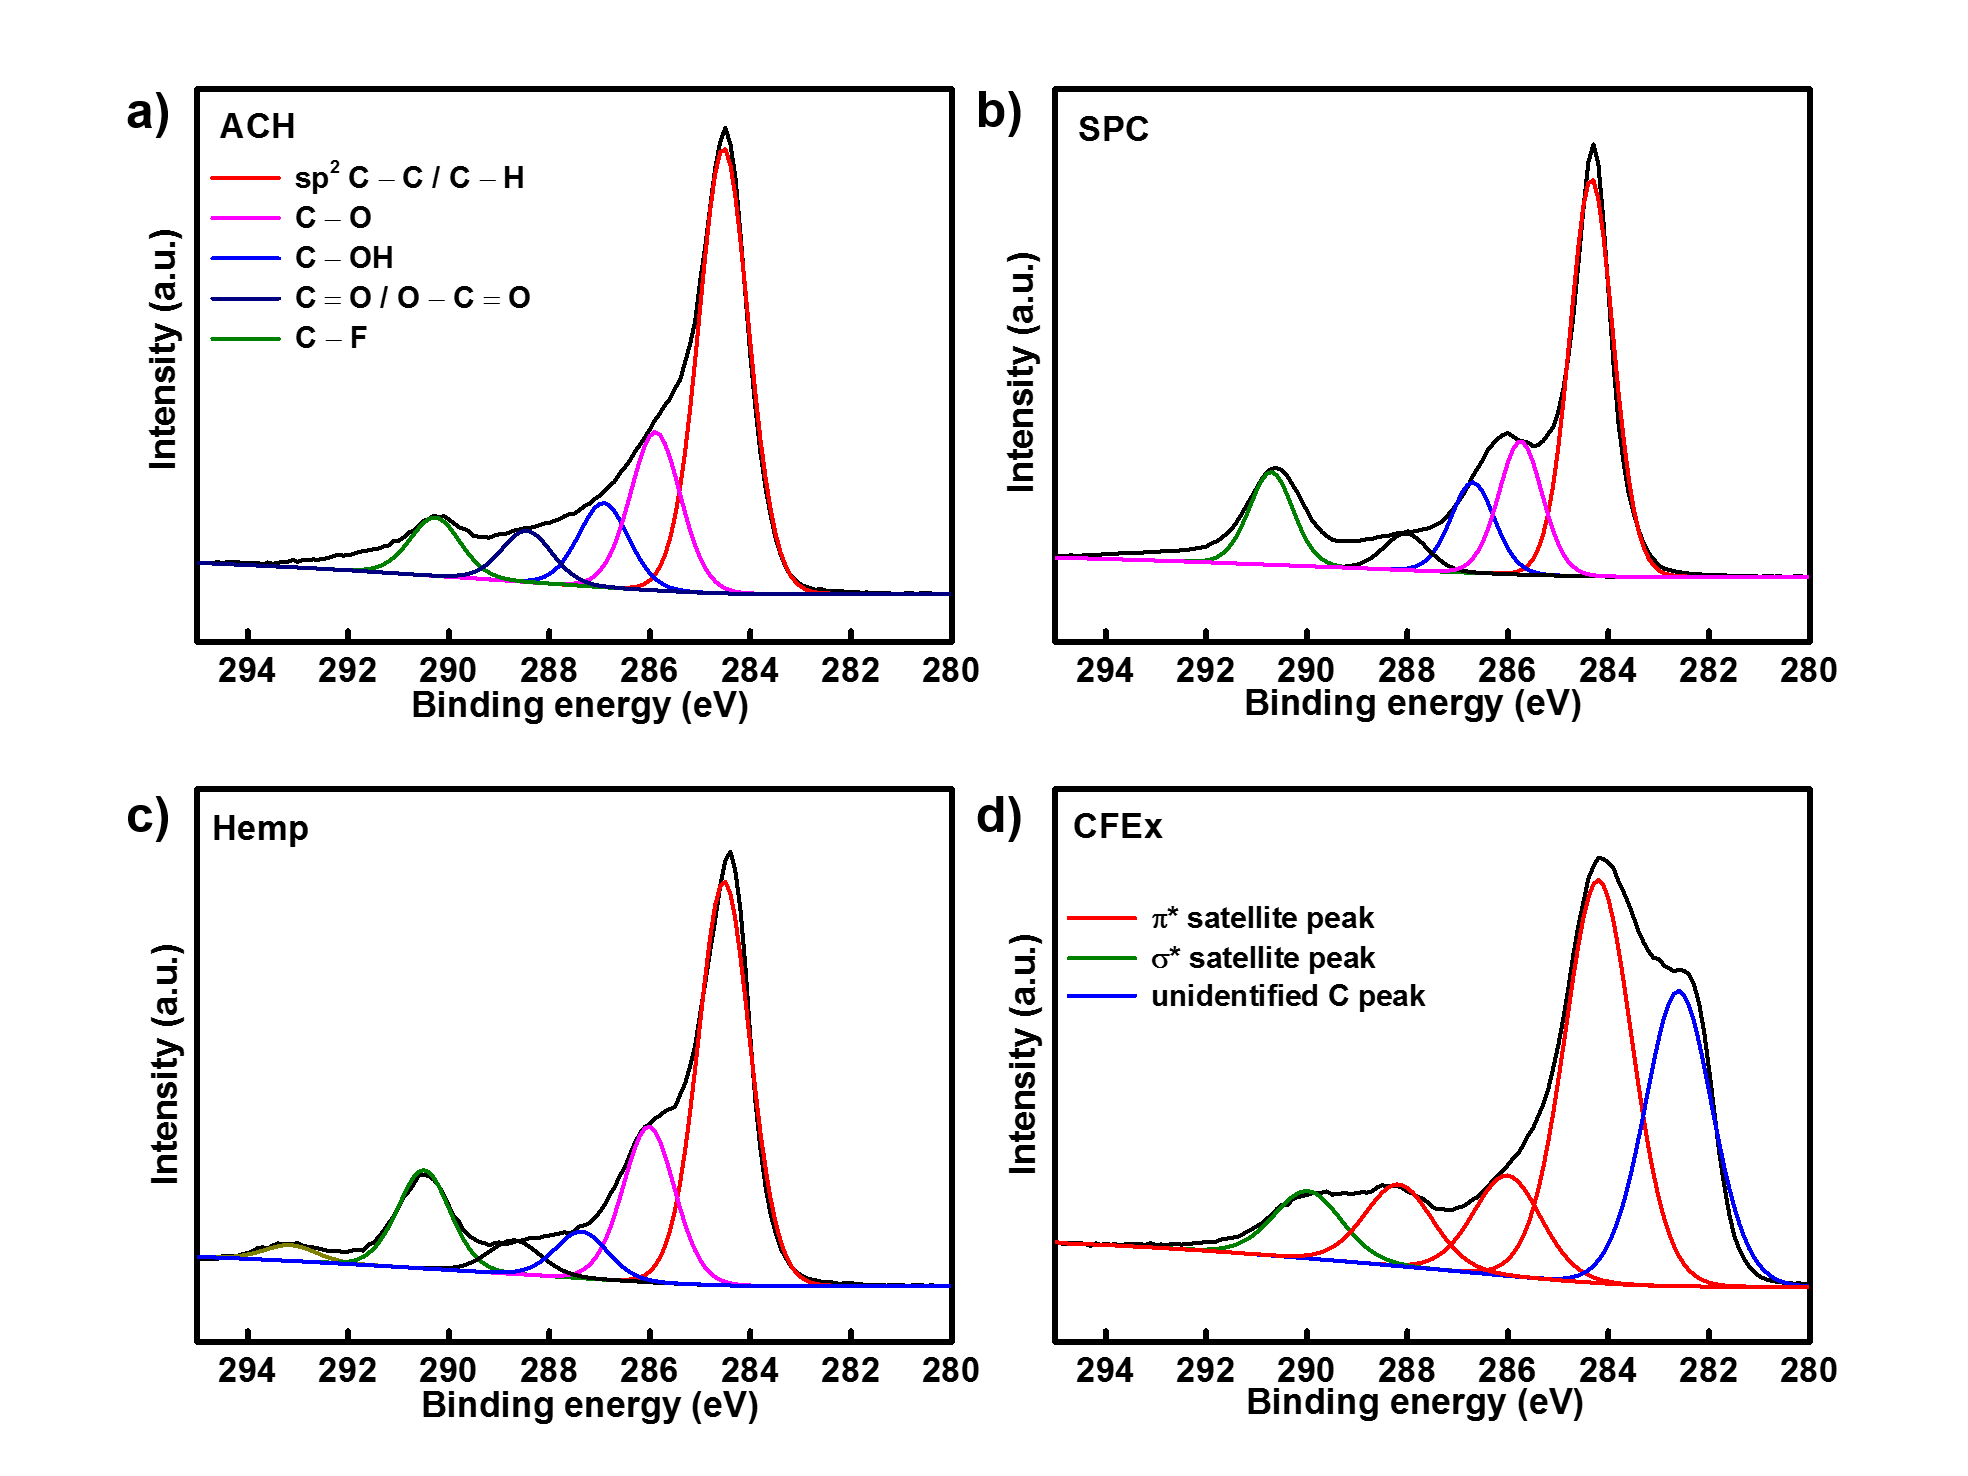
\includegraphics[width=\textwidth]{Figures/chap5fig/xpsc}
    \caption{Carbon 1s XPS spectra of pristine a) ACH, b) Super-P, c) hemp fibers and d) CFEx cathodes.While ACH, Super-P and hemp fibers observe carbonyl functional groups, CFEx cathodes have symmetrical looking $\pi$* and $\sigma$* satellite peaks.}
  \label{Figures/chap5fig:xpsc}
\end{figure}
We performed X-ray photoelectron spectroscopy on our cathodes to understand the kinds of reactions the cathodes could take part in. We observed ACH, hemp fibers and Super-P had similar looking peaks for carbon 1s orbital, Figure \ref{Figures/chap5fig:xpsc}. Peaks for sp$^2$ C-C/ C-H, C-O/ C-OH, O-C=O/ C=O and C-F bonds (formed between PVDF and the active material) appeared for ACH, hemp fibers and Super-P cathodes. To understand the presence of these bonds,we looked into the composition of these active materials. Hair is mainly composed of a protein called keratin displayed in Figure \ref{Figures/chap5fig:keratin}. Keratin constitutes of various C-H, C=O, C-OH and C-NH$_2$ bonds with their respective binding energies as observed in Figure \ref{Figures/chap5fig:xpsc}a. Sulphur is an essential part of this protein, a C-S bond can be observed at 286.94 eV (blue peak). 
\begin{table}
\caption{XPS data sheet for the tested cathodes with \textbf{Carbon 1s} peaks pointing C-H/ C-C, C-O/ C-OH, C=O/ O-C=O and C-F bonds, \textbf{Nitrogen 1s} peaks for pyrrolic and pyridnic N nods and \textbf{Oxygen 1s} peaks for aliphatic C-O and aromatic C=O peaks.} \label{table2}
\begin{tabular}{cccccccc}
\hline
Active & C-H/ & C-O/ & C=O/ & C-F & Pyrrolic N/ & aliphatic C-O & aromatic C=O\\
material & C-C & C-OH & O-C=O & & Pyridinic N & & \\
\hline\\
ACH & 284.5 eV & 285.8 eV & 288.4 eV & 290.2 eV & 400.2 eV/ & 533.0 eV & 531.2 eV\\
& & & & & 398.3 eV & & \\
CFEx & 284.2 eV & 286.0 eV & 288.2 eV & 290.0 eV & 399.3 eV & 531.3 eV & 530.2 eV\\
Hemp fibers & 284.5 eV & 286.0 eV & 288.7 eV & 290.5 eV & 400.3 eV & 532.9 eV & 531.4 eV\\
Super-P & 284.3 eV & 286.7 eV & 288.0 eV & 290.7 eV & 400.2 eV & 532.8 eV & ---\\
\hline
\end{tabular}
\end{table}
The oxygen-containing carbonyl and ester groups improve the wettability of cathode materials. It increases the availability of active surface area for the ions from the electrolyte to interact with the carbon matrix \cite{younesi_analysis_2015}. This enhances the pseudocapacitance of the cell since most of the capacity comes from a surface-based charge storage mechanism. Pristine hemp fibers and Super-P observed peaks for both sp$^2$ bonded carbon atoms and carbon-oxygen bonds \cite{hussain_development_2019}. Hemp fibers are composed of proteins called lignin (Figure \ref{Figures/chap5fig:lignin}), edestin and albumin which constitutes of arginine (Figure \ref{Figures/chap5fig:arginine}) and glutamic acid (Figure \ref{Figures/chap5fig:gluacid}).  

Carbon 1s spectrum of Super-P consists of contribution from O–C–O and/or C=O bonds and a strong \ce{CH2}/\ce{CF2} bond. The material is produced from partial oxidation of petrochemical precursors exhibiting a large specific surface area and a very high electrical conductivity \cite{gnanamuthu_electrochemical_2011}. Carbon black consists of nearly spherical primary particles, which are fused together in form of aggregates. A perfect graphite surface containing only carbon atoms, without heteroatoms like oxygen and sulfur would give a very well-ordered structure. Therefore, presence of carbonyl groups created defects resulting in a less graphitic and more amorphous structure\cite{hao_carbonaceous_2013}. 
Carbon spectra for CFEx electrode was uniquely different with highly symmetrical peaks. The presence of $\pi$ electrons on fullerene's surface renders multiple $\pi$ satellite peaks. These peaks are characteristic signs of a \ce{C60} molecule \cite{skryleva_xps_2016}. The symmetrical peaks in the low energy range, 284–289 eV, have C 1s excitation to final states of $\pi$* character (in red), while the higher energy peaks appear due to C 1s excitation to final states of $\sigma$* character (in green) \cite{erbahar_spectromicroscopy_2016, poirier_carbon_1993}. %Existence of several peaks in the $\pi$ satellite of a C$_6_0$ molecule is caused by the angular quantisation of orbitals around the centre of the spherical molecule. 
%XPS analysis results... O 1s
\begin{figure}[tbh!]
  \centering
  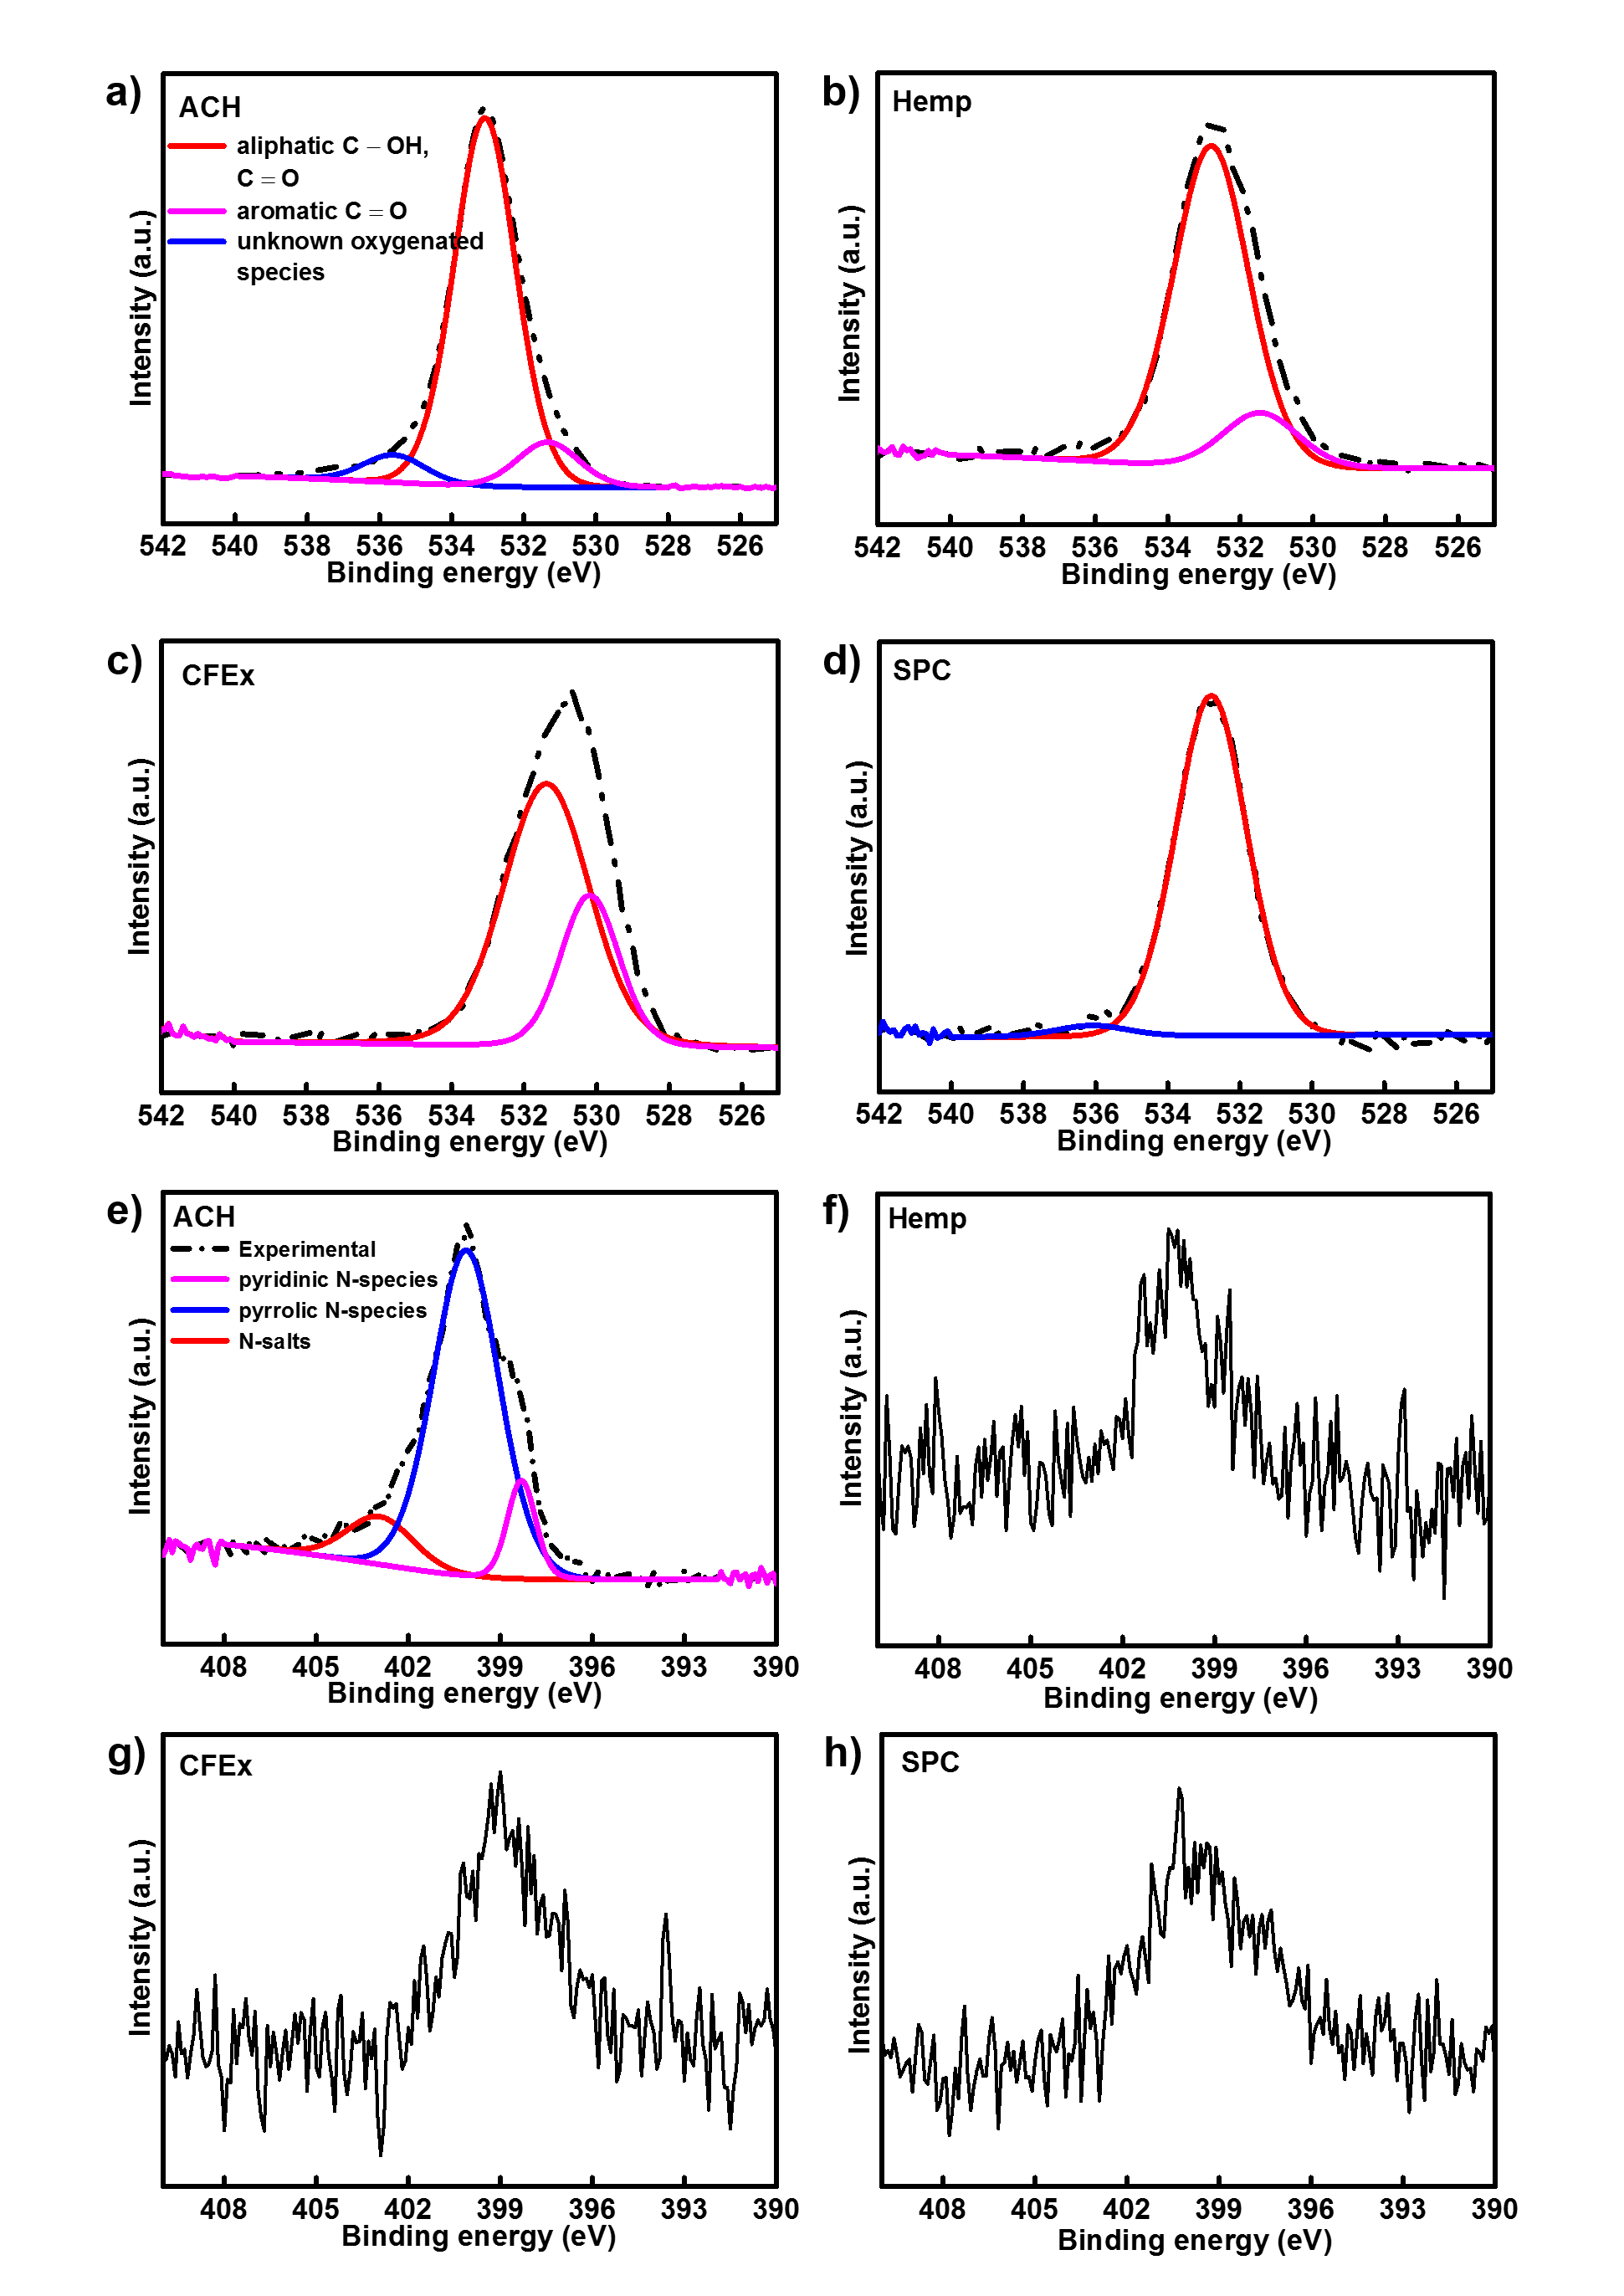
\includegraphics[width=0.8\textwidth]{Figures/chap5fig/xpson}
    \caption{Oxygen 1s orbital XPS spectra of a) ACH, b) hemp fibers c) CFEx and d) Super-P cathodes. ACH and hemp fibers have significant amounts of aliphatic (red) and aromatic (pink) C=O groups present on the cathode surface; while Super-P and CFEx have low amount of oxygenated species at their surface. Nitrogen 1s orbital XPS spectrum of e) ACH, f) hemp fibers g) CFEx and h) Super-P cathodes. ACH displays distinct binding energies for pyridinic and pyrrolic N-species; hemp fibers show lower amount of surface proteins, while Super-P and CFEx have low concentrations of N-containing functional groups.}
  \label{Figures/chap5fig:xpson}
\end{figure}
Figure \ref{Figures/chap5fig:xpson}a-d represents the oxygen 1s peaks of ACH, hemp fibers, CFEx and Super-P cathodes. The peaks at $\approx$ 531 eV stands for an aliphatic -C=O bond. Aromatic C-OH bond has a higher binding energy at $\approx$ 533 eV. The presence of these carbonyl groups not only enhance the wettability of the electrodes, but also suggest towards a Faradaic process\cite{}. 
SPC and CFEx recorded less intense peaks due to negligible amounts C=O and C-O bonds present on their surface.
Looking at the nitrogen spectra in Figure 20, ACH has a distinct presence coming from keratin. Pyrrolic N species have a binding energy at 400.1 eV whereas pyridinic N-species appear at 398.3 eV. Guengen \textit{et al.} suggested that adding nitrogen molecules changed the electron distribution of carbon materials, enhances the wettability of the active material and  contributes to its capacitance \cite{gueguen_xps_2016}. Presence of strong N 1s peaks (Figure \ref{Figures/chap5fig:xpson}e) suggests enhanced wettability of the ACH cathode compared to others, which improves its charge-storage capacity. This might be another reason why ACH cathode recorded a higher specific capacity than other cathodes. 
 \begin{figure}[tbh!]
  \centering
  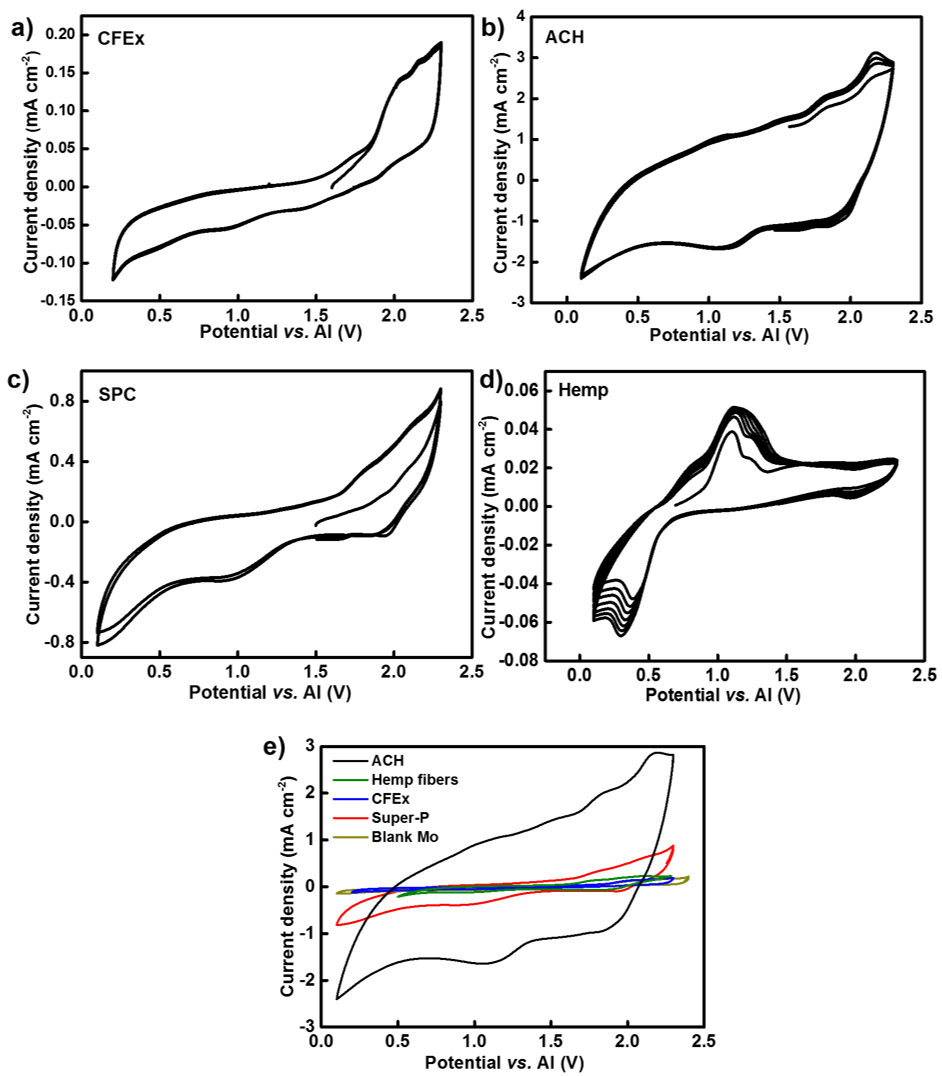
\includegraphics[width=\textwidth]{Figures/chap5fig/CV}
    \caption{Cyclic voltammograms of a) CFEx, b) ACH, c) Super-P and d) hemp fibers cathodes at a scan rate of 10 mV s$^{-1}$ against \ce{Al3+}/Al as a counter/reference electrode in a two-electrode setup. ACH cathode observed a larger CV area than other cathodes, which comes from an additional pseudocapacitance, adding capacity to the system.}
  \label{Figures/chap5fig:CV}
\end{figure}
Lastly, to confirm that ACH is surprisingly a psedocapacitive material, we compared cyclic voltammograms of all the cathodes at a scan rate of 10 mV s$^{-1}$. From Figure \ref{Figures/chap5fig:CV}a-e, it was seen that ACH had a rectangular CV curve. Intercalation process is noticeable at a lower sweep rate (10 mV s$^{-1}$) with tiny redox peaks visible (Figure \ref{Figures/chap5fig:CV}b). Redox pseudo-capacitance, which is usually observed at higher sweep rates (50 mV s$^{-1}$), can be seen in Figure \ref{Figures/chap5fig:hair50mVs}. Since \ce{AlCl4-} anions electrochemically absorb onto the surface of ACH, the  need for long-range diffusion of ions through van der Waals gap decreases. 

ACH proved to be the best carbon-based cathode among all the tested materials, with a specific capacity of 100 mAh g$^{-1}$ at a potential of 1.9 V with a coulombic efficiency of ~90$\%$. Intercalation and deintercalation of \ce{AlCl4-} takes place in the very few graphitic layers of ACH, hemp fibers and Super-P. 
We found that CFEx lacks a layered structure and it is mainly a cluster of \ce{C60} and \ce{C70} molecules. \ce{AlCl4-} anions seep in and out of the gaps in between the fullerenes changing its structure during insertion and expanding the crystal lattice (Figure \ref{Figures/chap5fig:cfexmech}). Since the cathode maintains its structural integrity, coulombic efficiency remains stable throughout the cycles for CFEx cell. Hemp fibers and Super-P on the other hand, have a highly amorphous structure and degrades after every cycle, resulting in a low capacity value. Figure \ref{Figures/chap5fig:cfexachlong} compares the 50th cycle measurement for Al/ACH and Al/natural graphite cell. It not only displays a higher specific capacity than conventional graphite, but also a high battery voltage of 1.92 V with an energy density of 202 Wh kg$^{-1}$.
 \begin{figure}[tbh!]
  \centering
  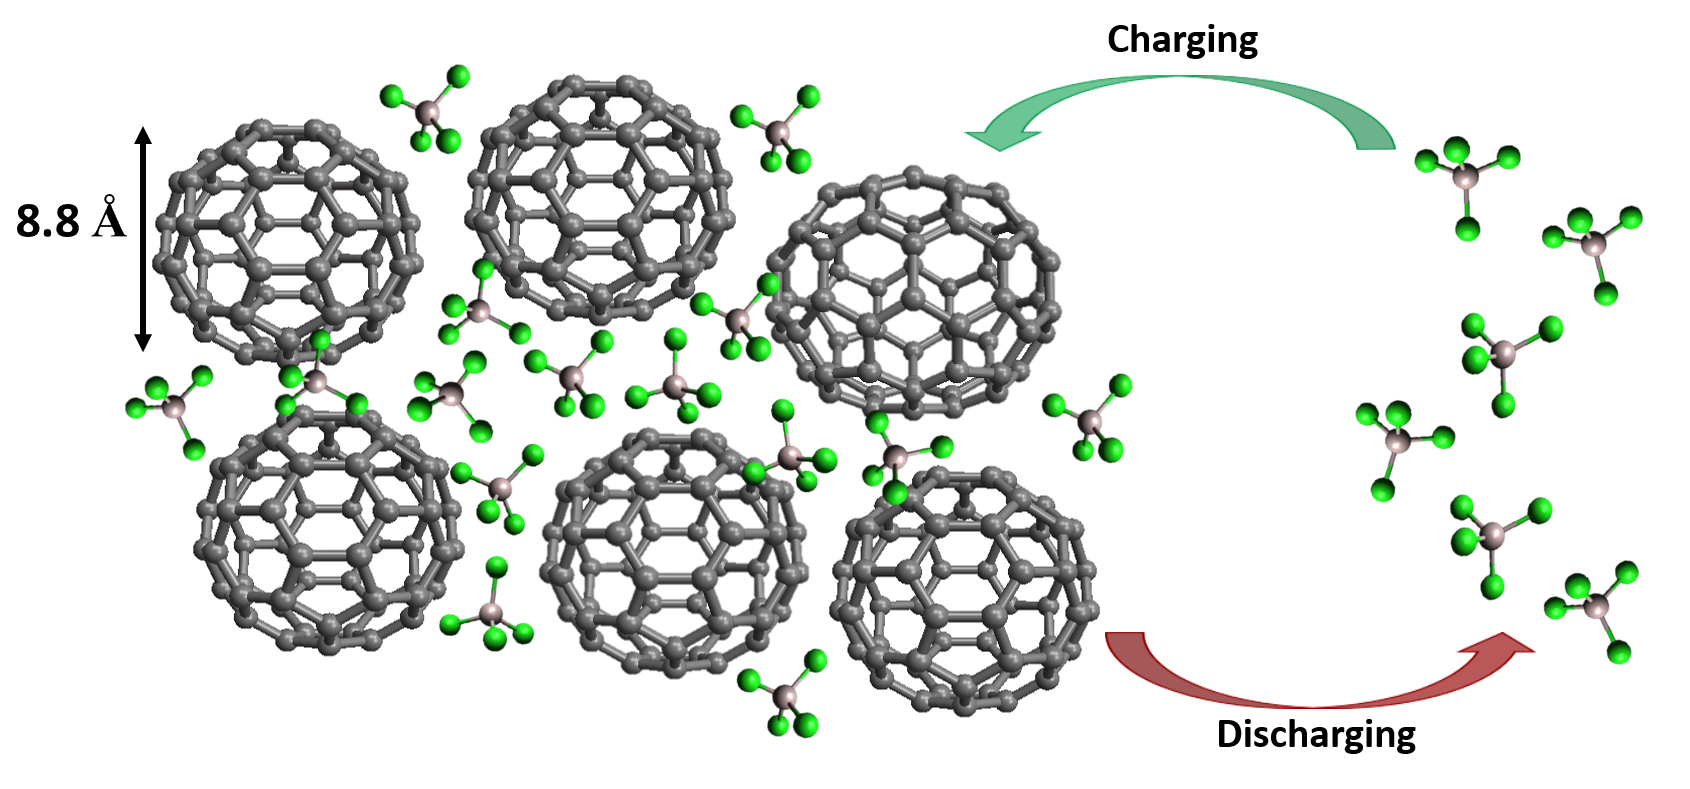
\includegraphics[width=\textwidth]{Figures/chap5fig/cfexmech}
    \caption{Suggested mechanism for a \textbf{Al/CFEx} cell. \ce{AlCl4-} ions seeping in through the gaps present between fullerene molecules. A few \ce{AlCl4-} ions get absorbed on the cathode's surface resulting in a capacity purely from a non-Faradaic process.}
  \label{Figures/chap5fig:cfexmech}
\end{figure}
\begin{figure}[tbh!]
  \centering
  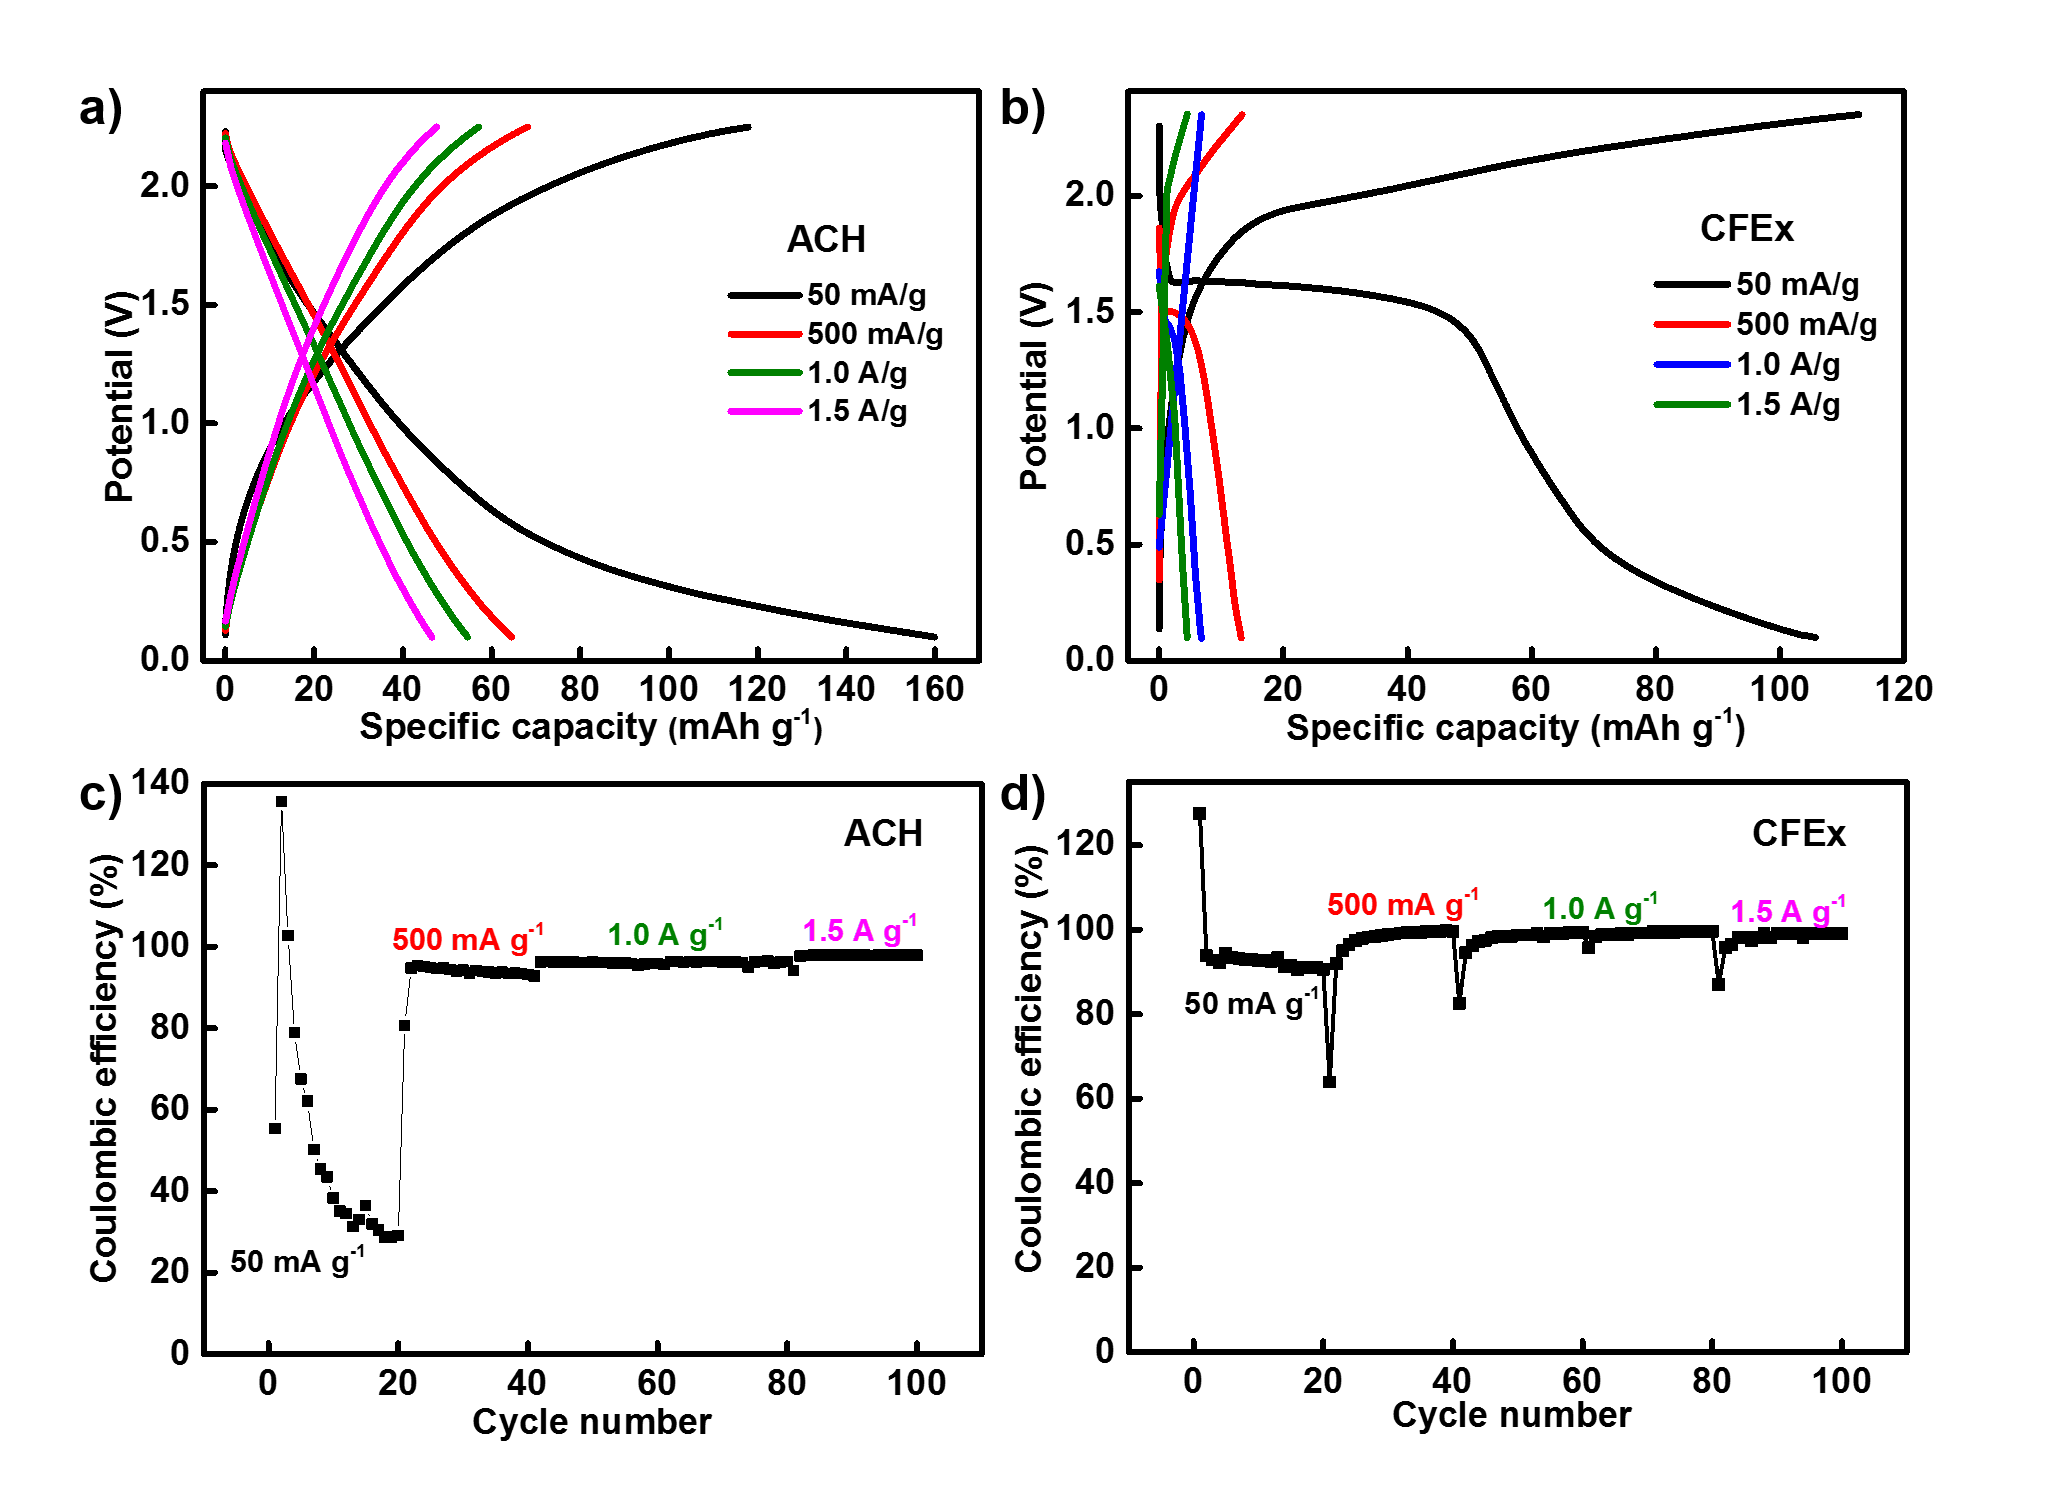
\includegraphics[width=\textwidth]{Figures/chap5fig/cfexachlong}
    \caption{Discharge capacities of a) ACH and b) CFEx cathodes at current rates of 50mAg$^{-1}$, 500mAg$^{-1}$, 1.0 Ag$^{-1}$ and 1.5 Ag$^{-1}$ along with their coulombic efficiencies. }
  \label{Figures/chap5fig:cfexachlong}
\end{figure}
\section{Experimental methods}
\subsection{Cathode preparation}
Slurry was prepared by mixing the active material (85$\%$ by wt.), 9$\%$ binder (PVDF, MTI Corp.) and 6$\%$ Super-P conductive carbon (99+$\%$ metals basis, Alfa Aesar) in N-methyl pyrrolidone NMP (anhydrous, 99.5$\%$, Sigma-Aldrich). For SPC slurry 94$\%$ active material and 6$\%$ binder was mixed together to form a slurry. It was ‘doctor-bladed’ on molybdenum foil used as a conductive substrate (thickness 0.1 mm, MTI Corp.) and dried in a vacuum oven at 120$^{\circ}$C for 12 hours to adhere the slurry on the substrate and evaporate the solvent. Specific loading of the materials ranged from 11-12 mg cm$^{-2}$. 
\subsection{Electrolyte preparation}
Anhydrous \ce{AlCl3} (Sigma-Aldrich) and EMImCl (97$\%$, Sigma-Aldrich) were mixed in a molar ratio of 1.3:1, at room temperature. EMImCl was baked in vacuum for 24 hours at 100$^{\circ}$C to remove residual moisture. Small aliquots of \ce{AlCl3} was added to EMImCl after every few minutes. The ionic liquid was stirred for 2-3 hours until a clear brown liquid was obtained. Since the electrolyte is hygroscopic in nature, it was prepared in a \ce{N2}-filled glove box with <0.1 ppm \ce{H2O}/\ce{O2}. 
\subsection{Cell assembly}
PEEK (polyether ether ketone) cells were used for electrochemical measurements. Molybdenum rods were used as current collectors. It was seen previously that steel rods reacted with the electrolyte forming a green-colored substance on the cathode. Slurry coated on molybdenum foil was used as the cathode and placed at bottom of the cell. Two glass microfibers (Grade GF/F, Whatman) were used as separators. 80$\mu$l of the electrolyte was used to wet the separator. Aluminium foil (thickness 0.1 mm, 99$\%$, GoodFellow) used as an anode and placed on top of the separator. It was assembled in a \ce{N2}-filled glove box. The cell was then sealed and wrapped with a paraffin film to avoid any air or moisture contact. Since this was a two-electrode setup, aluminium foil was used as both counter and reference electrode. The cell was taken out of the glove box and electrochemical measurements were performed. 
\begin{figure}[tbh!]
  \centering
  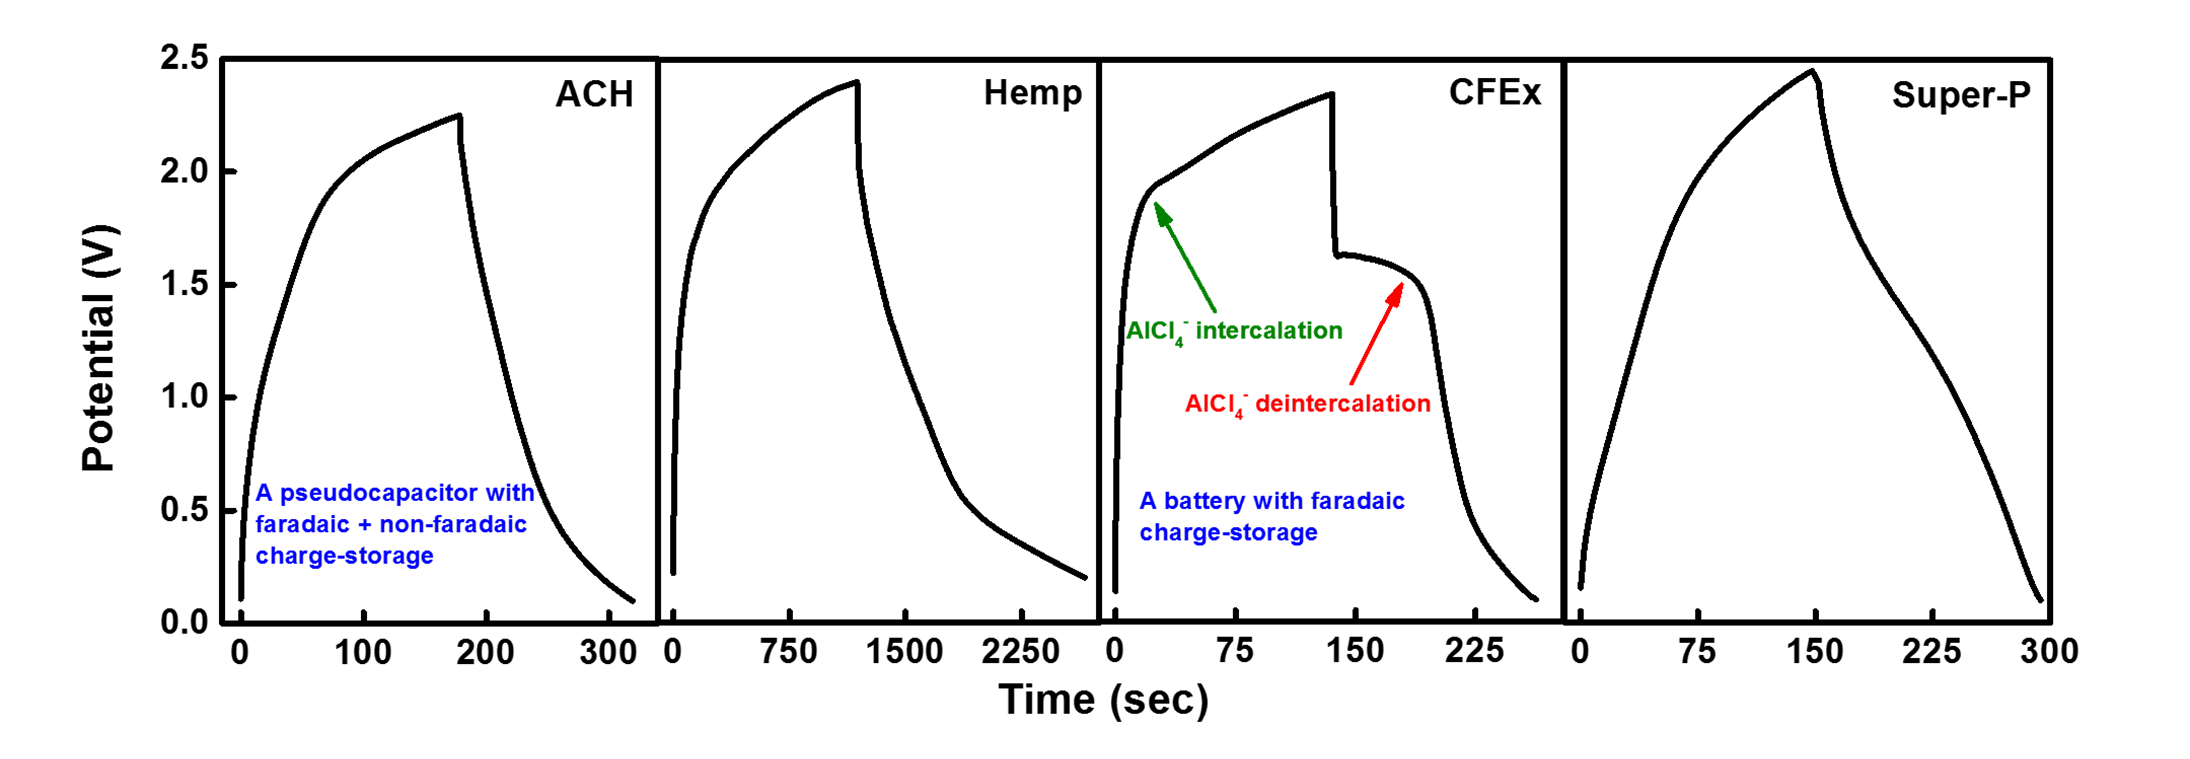
\includegraphics[width=\textwidth]{Figures/chap5fig/gcdall}
    \caption{Chronopotentiographs (Voltage vs. Time) curves of all tested cathodes.}
  \label{Figures/chap5fig:gcdall}
\end{figure}

\newcommand{\beginsupplement}{
               \setcounter{figure}{0}
        \renewcommand{\thefigure}{S\arabic{figure}}
     }
\beginsupplement
\begin{figure}[tbh!]
  \centering
  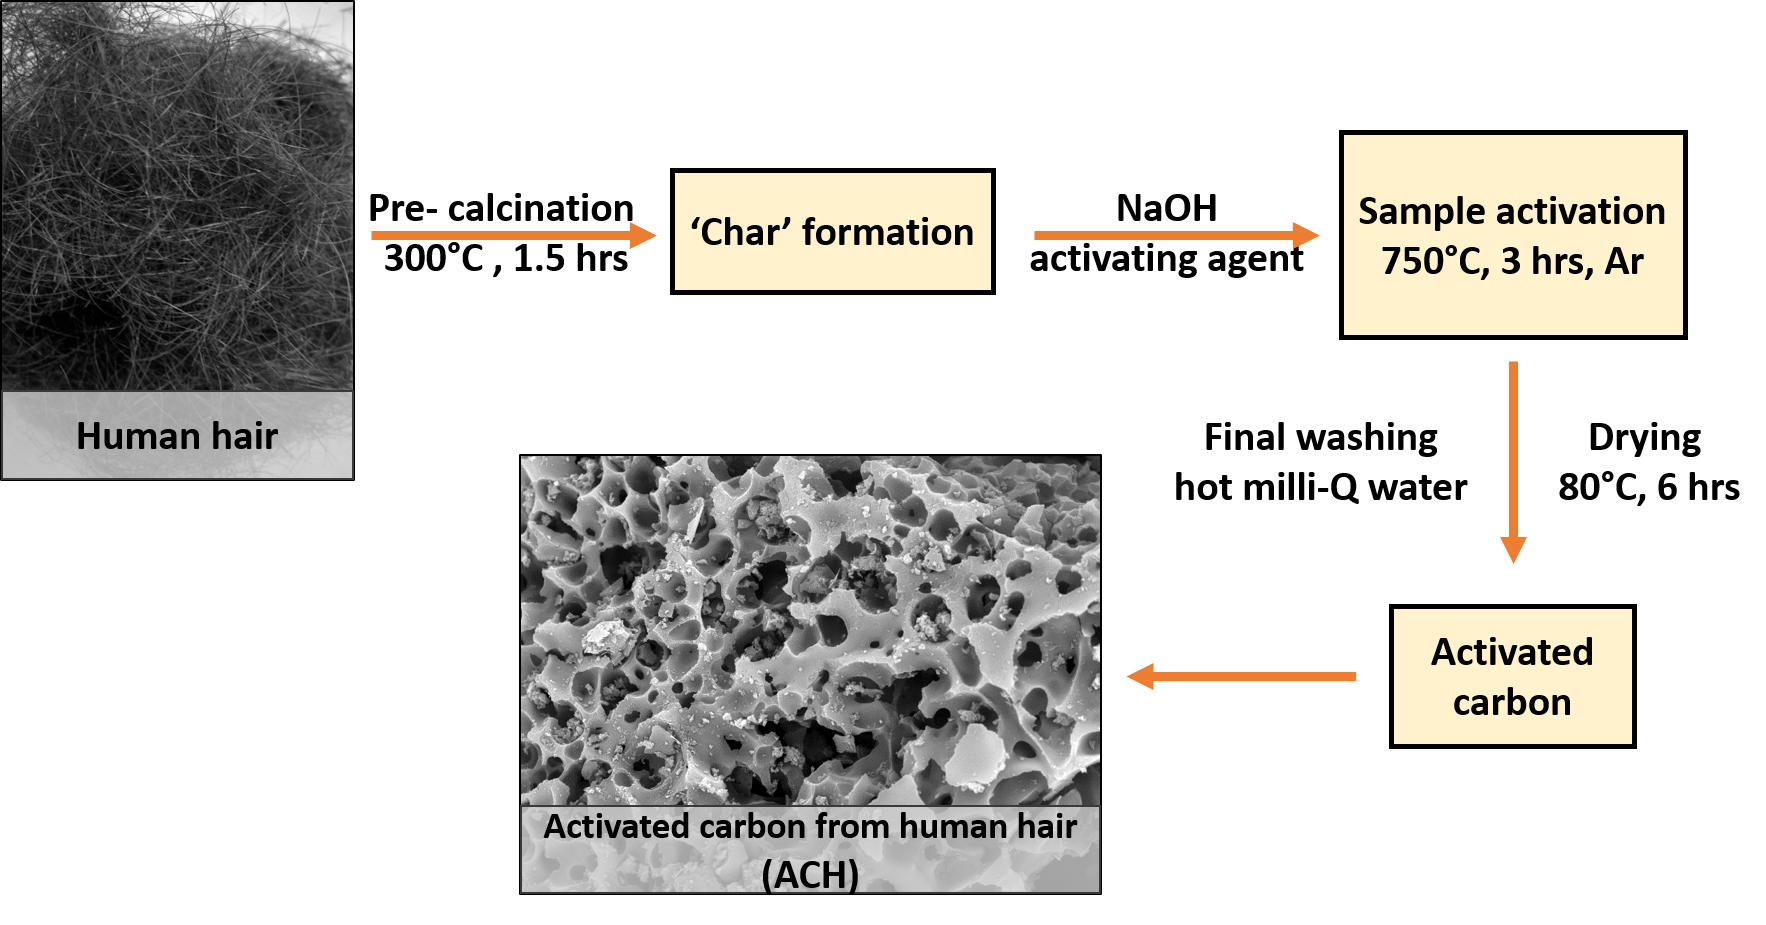
\includegraphics[width=\textwidth]{Figures/chap5fig/achsyn}
    \caption{Synthesis of activated carbon from human hair using NaOH as the activating agent. The choice of temperature and activating agent plays a crucial role in determining pore size of the activated carbon.}
  \label{Figures/chap5fig:achsyn}
\end{figure}
\begin{figure}[tbh!]
  \centering
  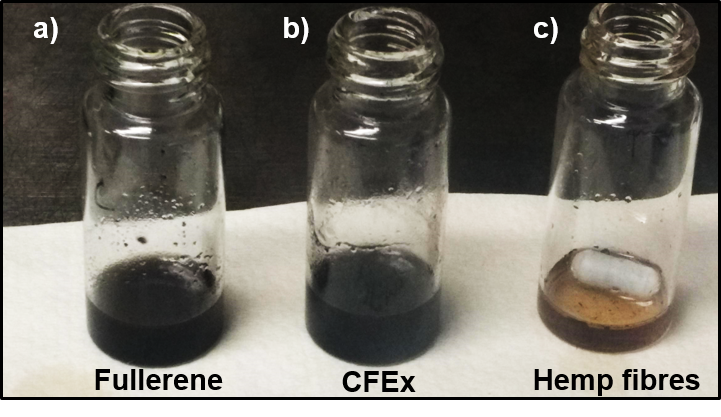
\includegraphics[width=\textwidth]{Figures/chap5fig/cfexsol}
    \caption{Synthesis of activated carbon from human hair using NaOH as the activating agent. The choice of temperature and activating agent plays a crucial role in determining pore size of the activated carbon.}
  \label{Figures/chap5fig:cfexsol}
\end{figure}
\begin{figure}[tbh!]
  \centering
  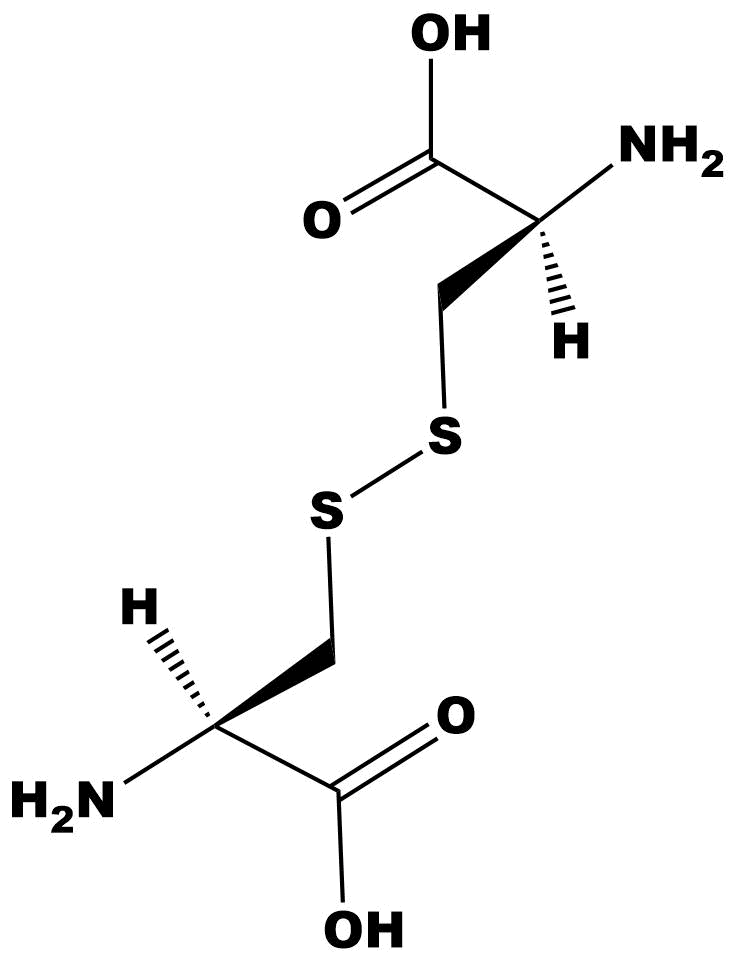
\includegraphics[width=0.5\textwidth]{Figures/chap5fig/keratin}
    \caption{Keratin: a protein abundantly found in human hair contains C-O, C=O, C-NH$_2$ bonds.} 
    \label{Figures/chap5fig:keratin}
\end{figure}
\begin{figure}[tbh!]
  \centering
  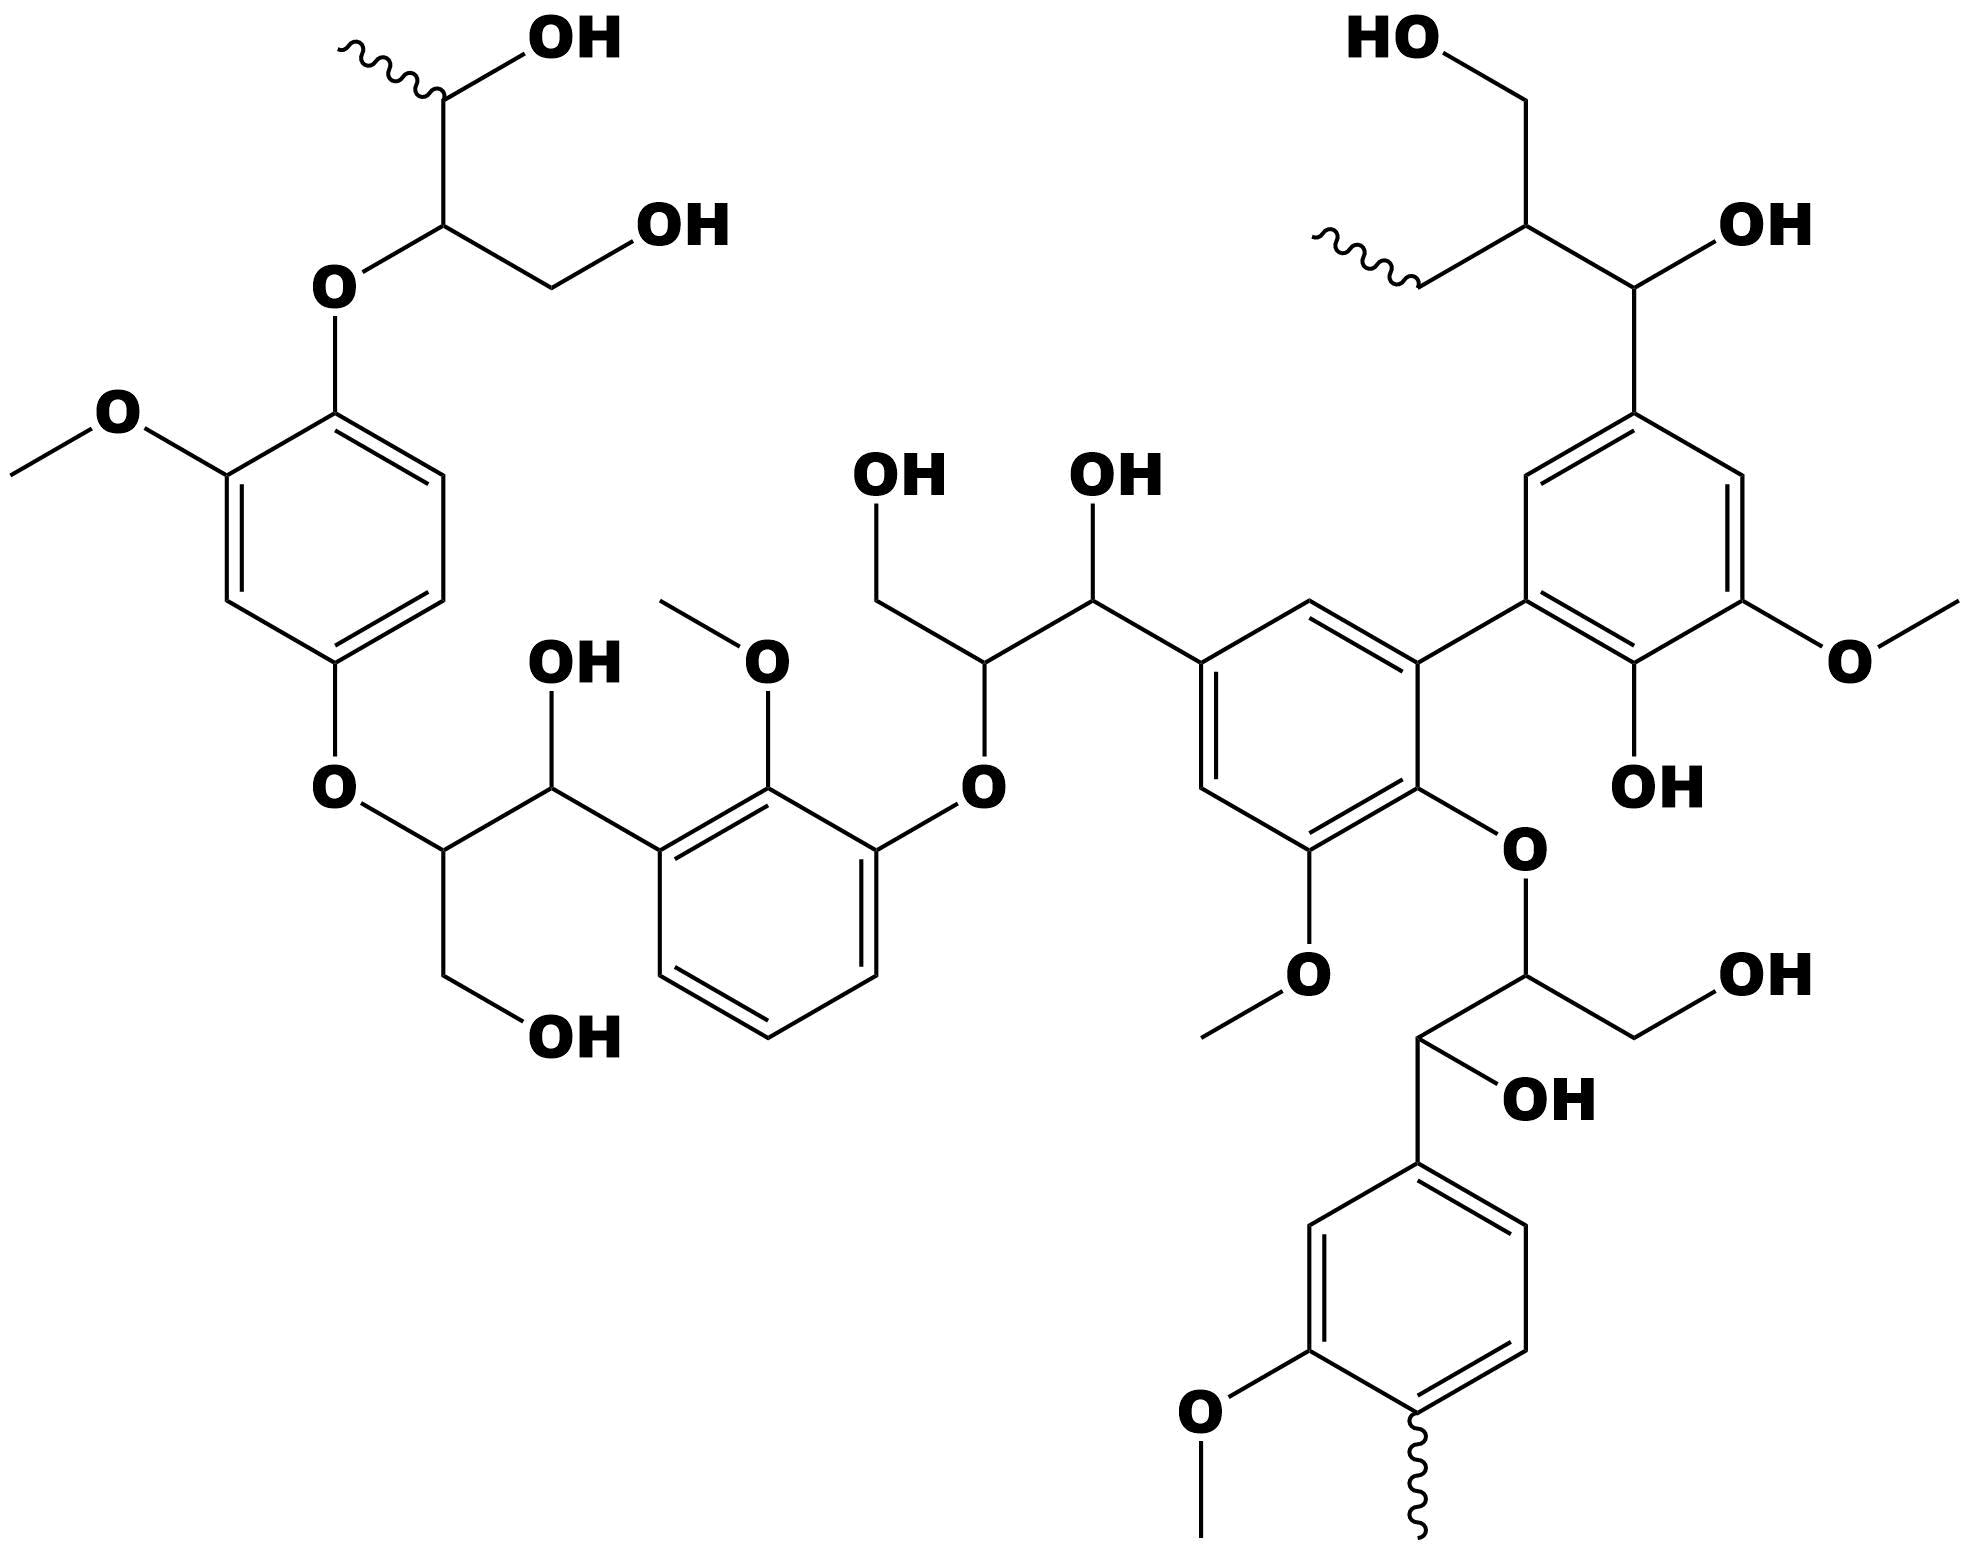
\includegraphics[width=0.5\textwidth]{Figures/chap5fig/lignin}
    \caption{Structure of Lignin- The lignin content of hemp will vary according to the part of the plant under observation. It contains a number of carbonyl, ester groups along with other proteins such as edestin and albumin.}
  \label{Figures/chap5fig:lignin}
\end{figure}
\begin{figure}[tbh!]
  \centering
  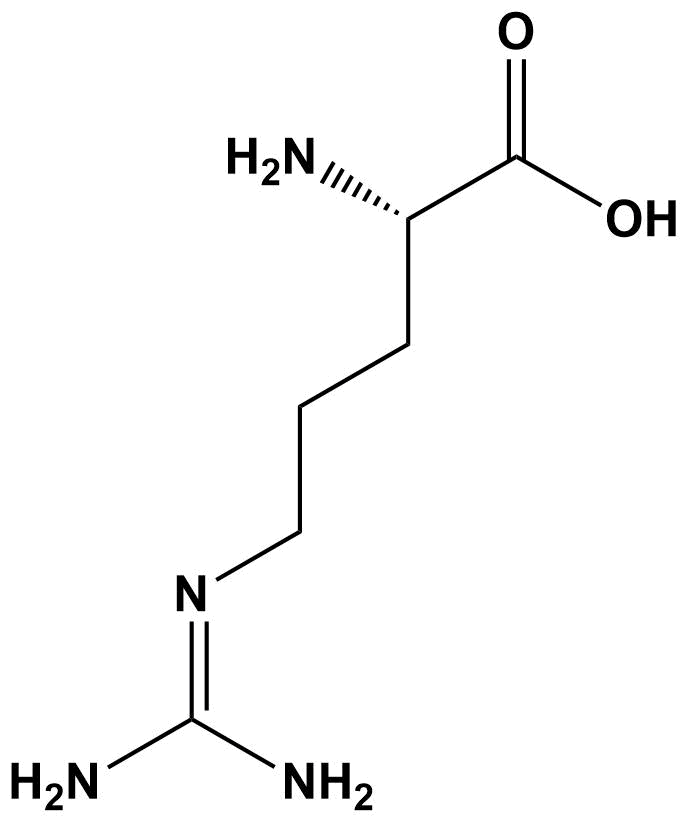
\includegraphics[width=0.5\textwidth]{Figures/chap5fig/arginine}    
  \caption{Structure of Arginine- major component of hemp fibers containing C-N, C=O, C-O bonds.}
  \label{Figures/chap5fig:arginine}
\end{figure}
\begin{figure}[tbh!]
  \centering
  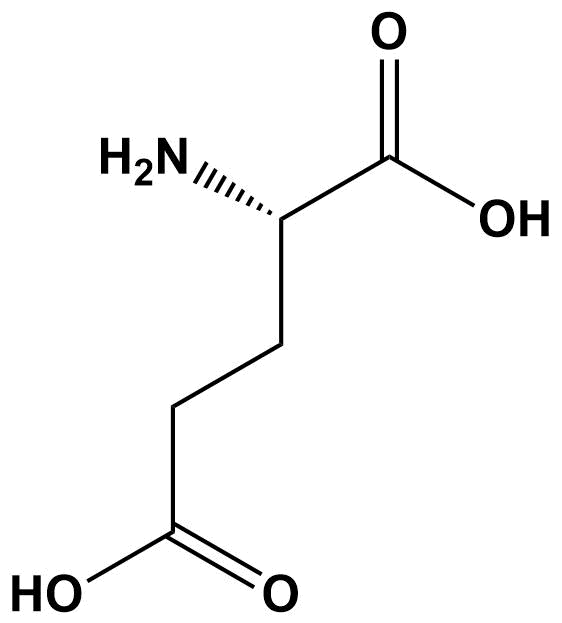
\includegraphics[width=0.5\textwidth]{Figures/chap5fig/gluacid}
    \caption{Structure of Glutamic acid- another protein found in hemp fibers containing C-O, C=O and C-N bonds.}
  \label{Figures/chap5fig:gluacid}
\end{figure}
\begin{figure}[tbh!]
  \centering
  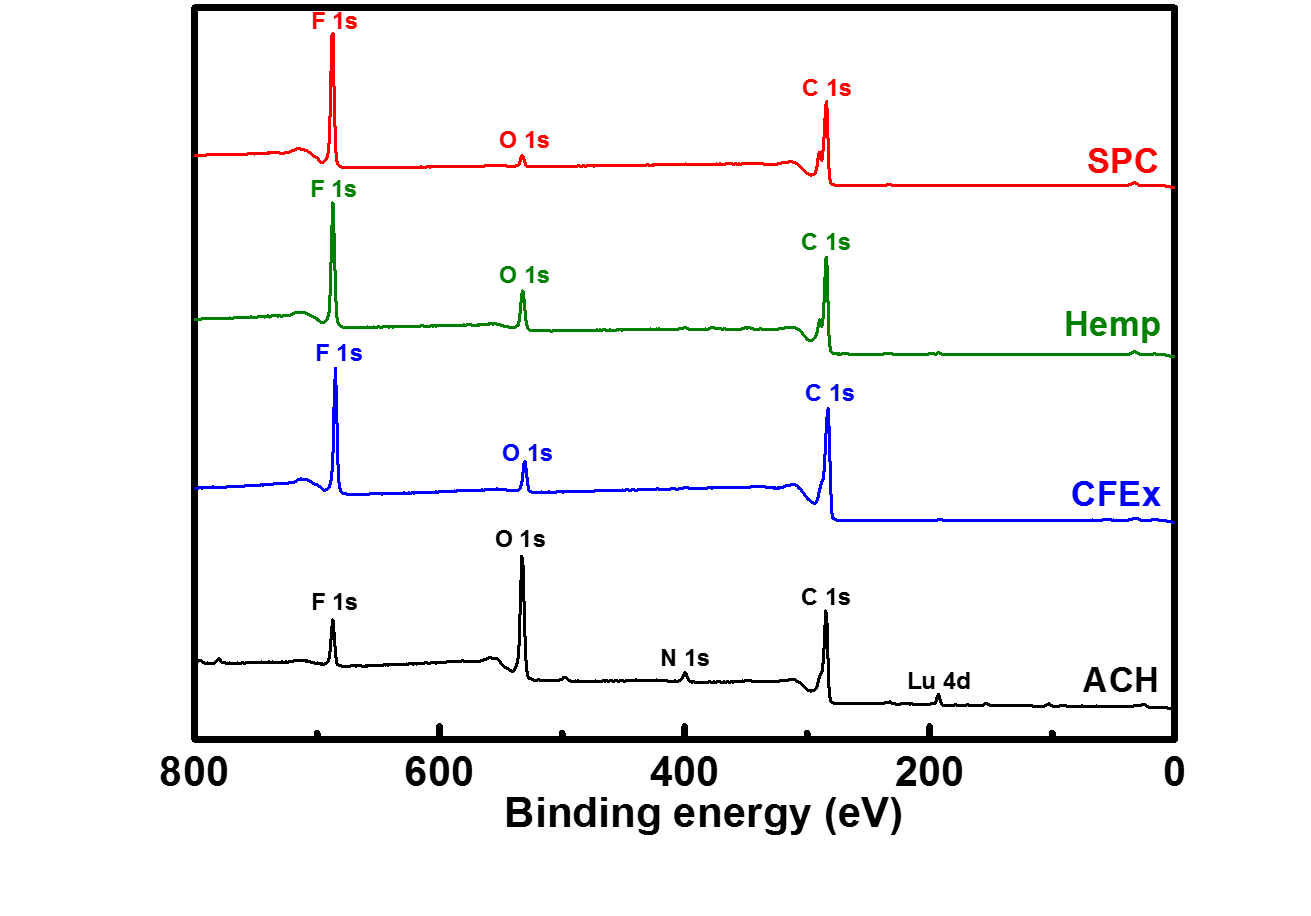
\includegraphics[width=\textwidth]{Figures/chap5fig/xpsoverall}
    \caption{Overall spectra of ACH (blck), hemp fibers (blue), CFEx (green) and SUper-P(red).}
  \label{Figures/chap5fig:xpsoverall}
\end{figure}
\begin{figure}[tbh!]
  \centering
  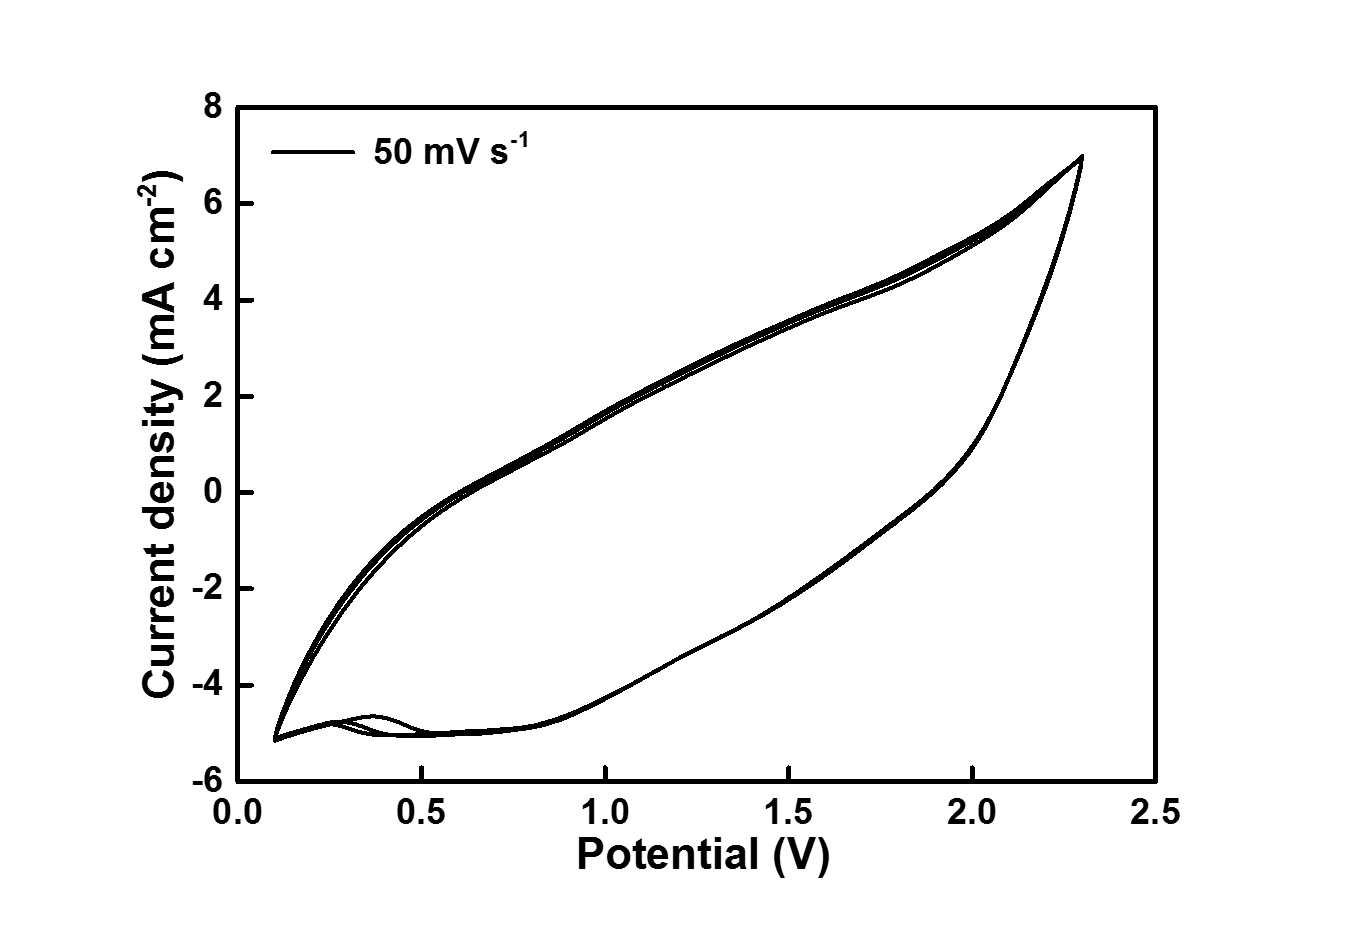
\includegraphics[width=\textwidth]{Figures/chap5fig/hair50mVs}
    \caption{Cyclic voltammogram of ACH at a scan rate of 50 mV/s in a two electrode setup against \ce{Al3+}/Al showing a capacitor-like behaviour with no visible oxidation-reduction peaks unlike Figure \ref{Figures/chap5fig:CV}b where we distinctly observed redox peaks.}
  \label{Figures/chap5fig:hair50mVs}
\end{figure}
\section{Conclusion and future outlook}

 
%\section*{Preface}
This chapter is about discovering a material which achieved one of the highest specific capacities for non-aqueous aluminium-ion batteries! Boron nitride was tested as a cathode material and it showed a very high discharge capacity (>250 mAh g$^{-1}$). However, it turned out that boric anhydride (\ce{B2O3}), which was an impurity in hexagonal boron nitride (hBN), was the active material. Pure \ce{B2O3} was tested as a cathode material, the battery produced a similar discharge capacity of >250 mAh g$^{-1}$.   

\begin{figure}[tbh!]
\centering
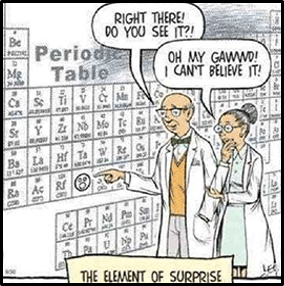
\includegraphics[width=\textwidth]{Figures/BOhBN/ah}
\end{figure}

\newpage
\chapter{Boron nitride/boron oxide as a cathode for rechargeable AIBs} 
\label{BOhBN} 

\section{Theory and background}

\begin{figure}[tbh!]
\centering
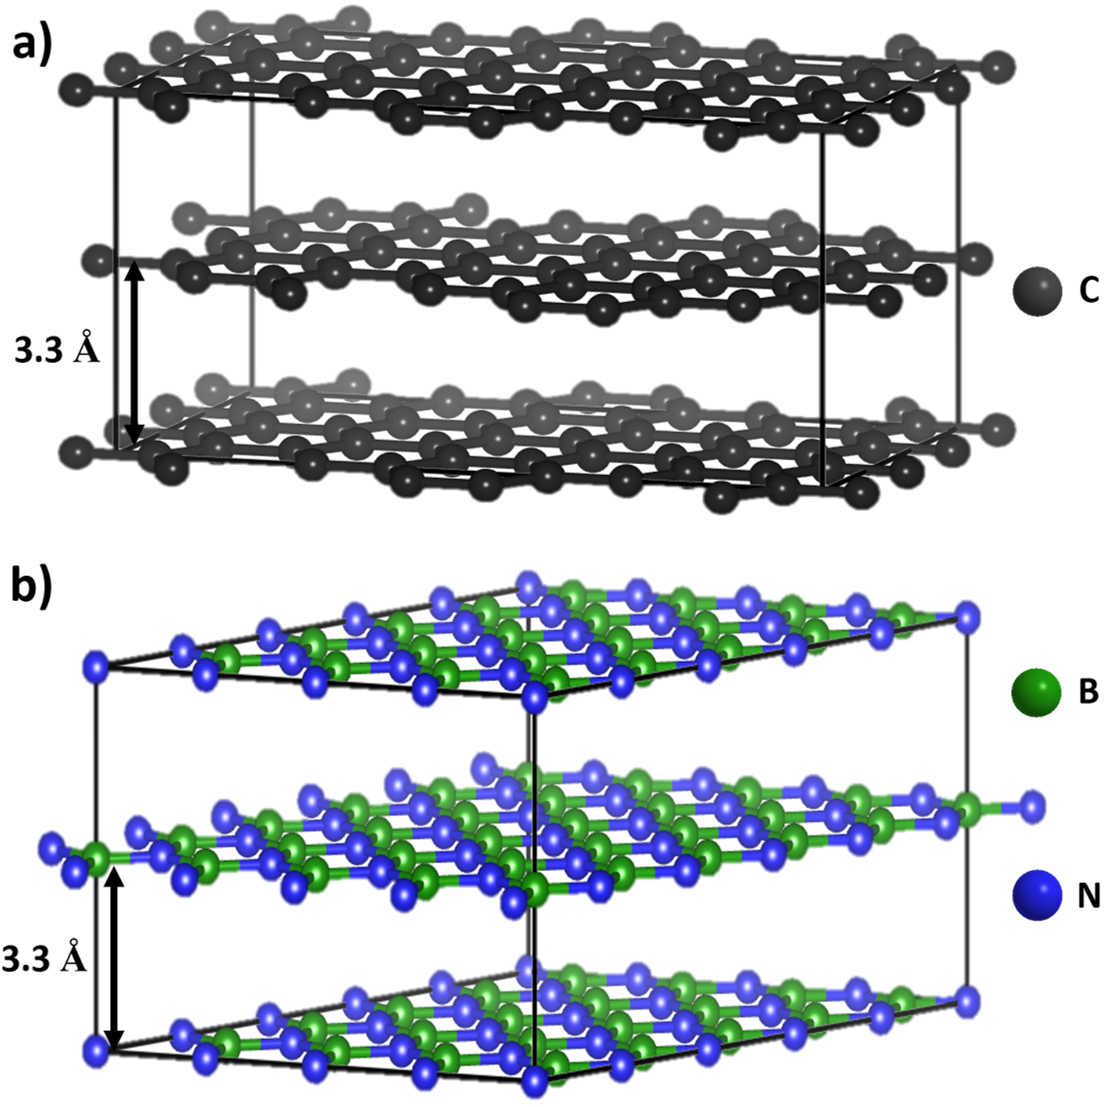
\includegraphics[width=\textwidth]{Figures/BOhBN/grpBNcomp}
\caption{Honeycomb lattice of a) natural graphite and b) hexagonal boron nitride. Both structures display an interlayer distance of 3.3\AA.}
\label{Figures/BOhBN:grpBNcomp}
\end{figure}

Graphite has been extensively used as a cathode in AIBs due to its high conductivity and its layered structure. Graphite and hexagonal boron nitride (hBN) are materials that possess a hexagonal lattice structure \cite{hod_graphite_2012}. hBN is also known as inorganic graphite. Where graphite has non-polar homonuclear C-C intralayer bonds, hBN on the other hand displays highly polar B-N bonds. In the bulk form, the two materials have different stacking modes. Furthermore, the static polarizabilities of the constituent atoms are significantly different, suggesting large differences in the dispersive component of the interlayer bonding\cite{song_large_2010, zeng_white_2010}. Despite these major differences, both materials present practically identical interlayer distances as shown in  Figure \ref{Figures/BOhBN:grpBNcomp}. Structurally, a single layer of hBN is very similar to a graphene sheet and has a hexagonal backbone where each couple of bonded carbon atoms is replaced by a boron nitride pair, making the two materials isoelectronic. Nevertheless, due to the electronegativity differences between the boron and the nitrogen atoms, the $\pi$ electrons tend to localize around the nitrogen atomic centers, thus making it an insulating material. The nature of bonding between nitrogen and boron differs from the carbon-carbon bonds found in graphite. hBN possesses coordinate bonds resulting from donation of \ce{e-} pair from nitrogen into empty p-orbital of a neighbouring B atom. Each N atom develops a partial positive charge and each B develops a partial negative charge. The partial ionic character of BN bonding makes it a semi-conductor as opposed to a conductor like graphite. hBN has been used in solid-state LIBs in various forms. When it is mixed with the electrolyte, it imparts exceptional thermal stability that allows high-rate operation of solid-state rechargeable LIBs at temperatures up to 175 $^{\circ}$C\cite{hyun_high}. When coated onto the surface of a poly(ethylene oxide) (PEO)-based electrolyte, hBN formed a robust interfacial layer to improve the chemical and mechanical stability of the PEO-based electrolyte, leading to the enhanced performance of solid-state Li metal batteries\cite{shen_chem}. Boron nitride nanotubes (BNNTs) were synthesized by Rahman \textit{et al.} and used for the modification of a polyolefin separator without blocking the porous channels of the conventional separator for \ce{Li+} ion diffusion. This improved the thermal stability up to 150 $^{\circ}$C \cite{rahamn_}.\\*
For the above mentioned advantages, hBN was considered as a cathode for AIBs. Despite the fact that hBN is an insulator, it was assumed that additives like conductive carbon (Super-P) would compensate for the loss of conductivity. In addition, hBN was a new material in the field of AIBs.\\* 

\section{Results and discussion}

\begin{figure}[tbh!]
\centering
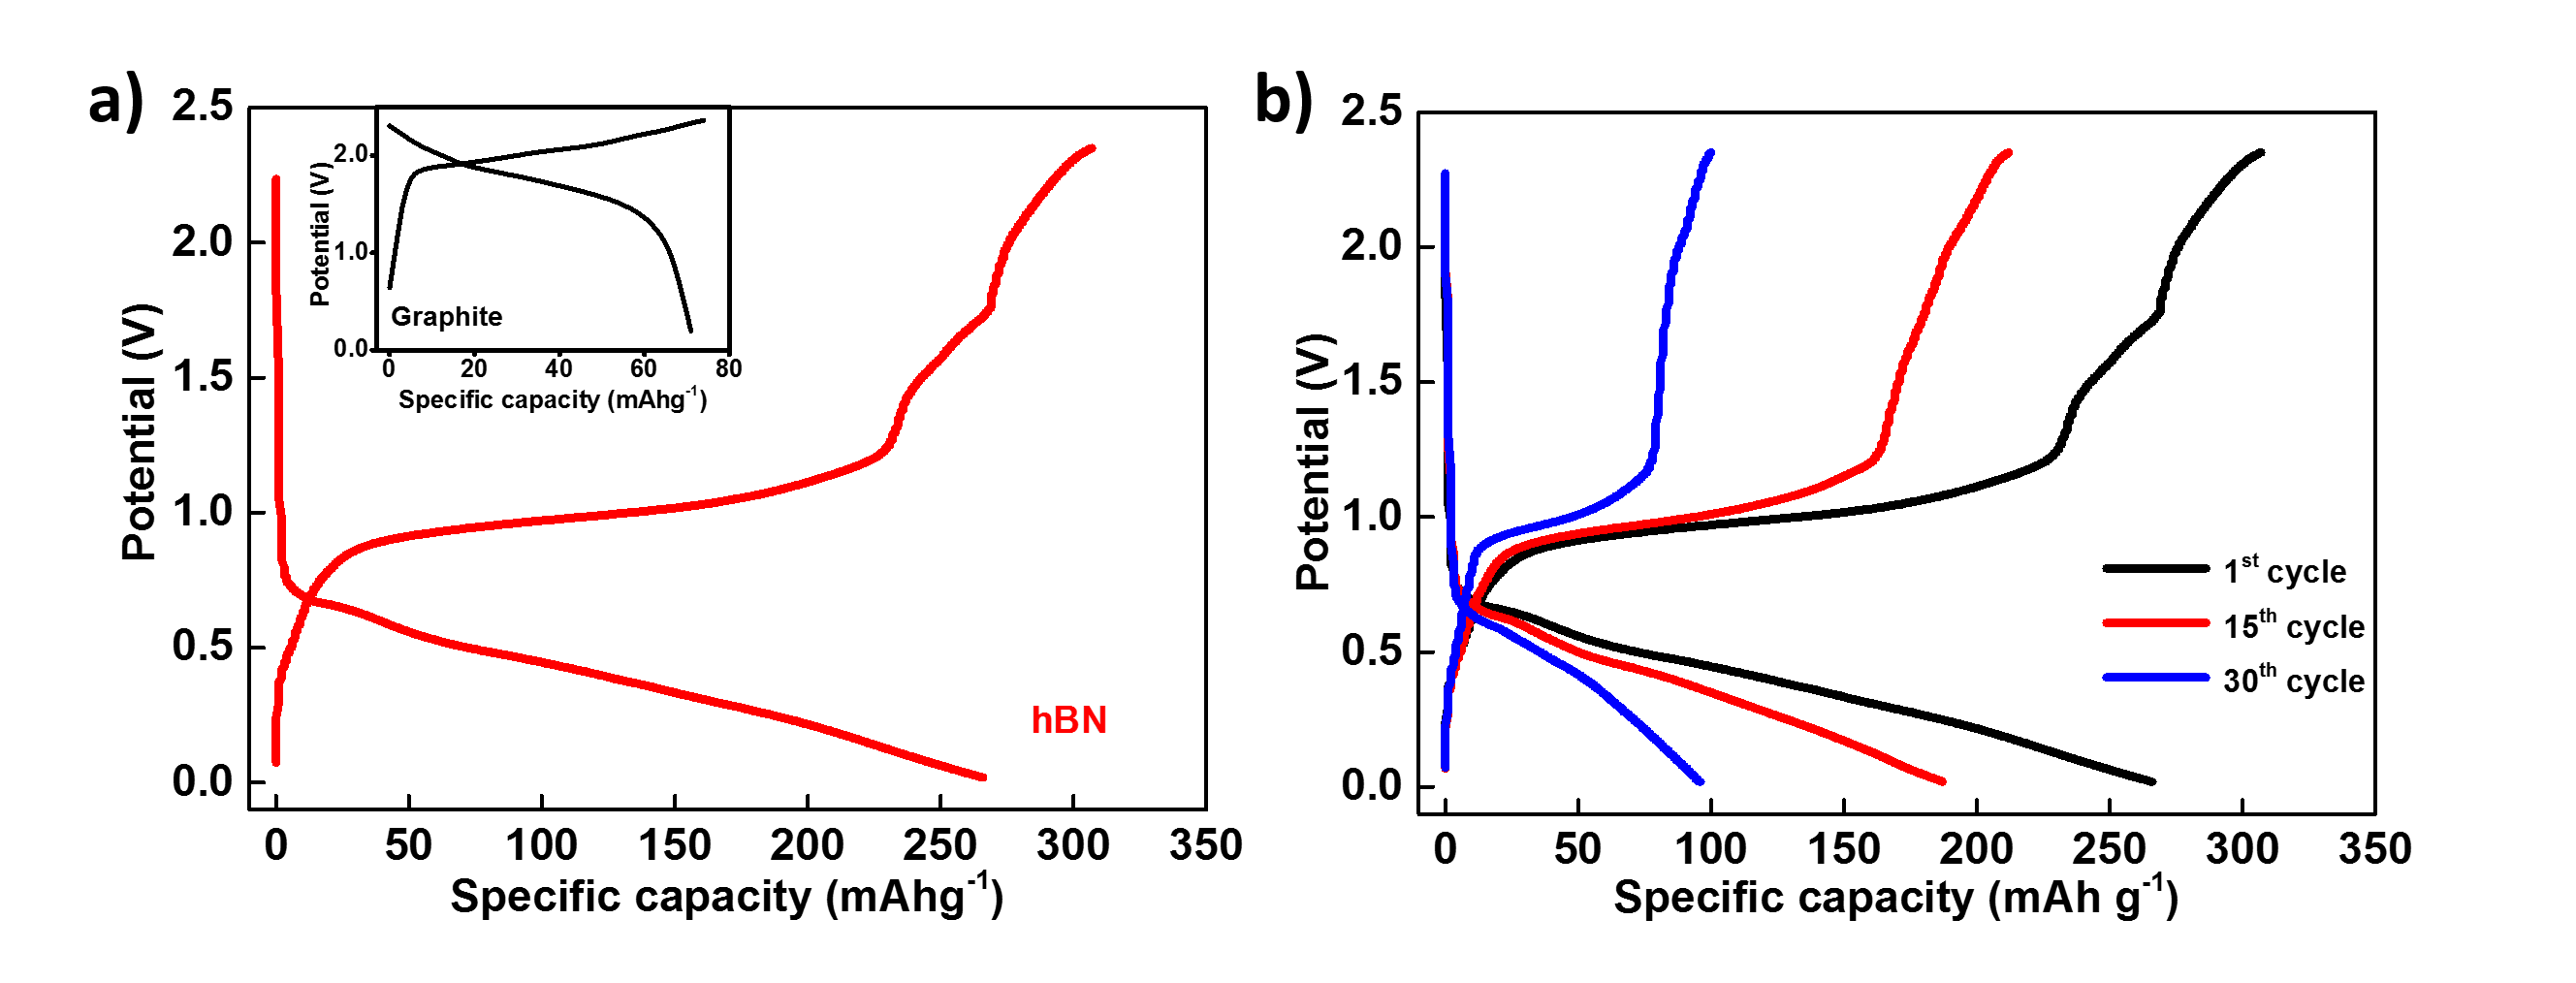
\includegraphics[width=\textwidth]{Figures/BOhBN/hBNiniCDC}
\caption{a) Galvanostatic cycles of an Al/hBN, using hBN from the stores (with \ce{B2O3} as an impurity), at a current density of 50 mA g$^{-1}$ compared with natural graphite (inset). b) Capacity fading of Al/hBN cell recorded for 30 cycles at a current rate of 50 mA g$^{-1}$.}
\label{Figures/BOhBN:hBNiniCDC}
\end{figure}

\begin{figure}[tbh!]
\centering
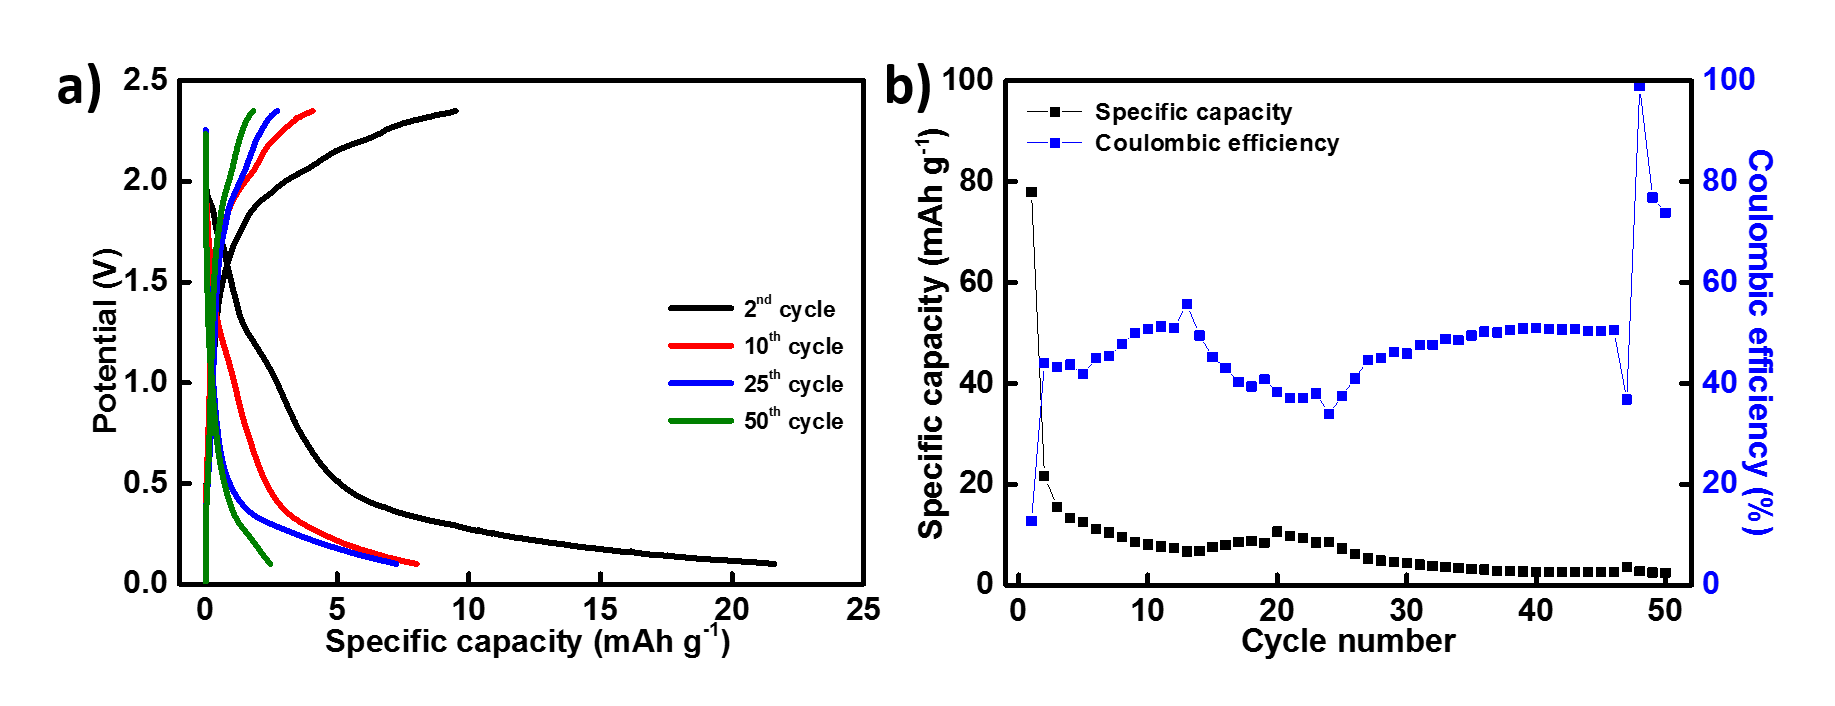
\includegraphics[width=\textwidth]{Figures/BOhBN/BNNSCDCCE}
\caption{a) Performance of an aluminium-ion battery using pure hBN as cathode at a current rate of 50 mA g$^{-1}$. b) Discharge capacity drops down to 5 mAh g$^{-1}$ after 50 cycles. hBN displays a very low coulombic efficiency $\approx$ 55\%.}
\label{Figures/BOhBN:hBNCDCCE}
\end{figure}

For all the above mentioned reasons, we tested hBN as a cathode for AIBs. To save cost, an old bottle of hBN was retrieved from VUW's chemical stores. A cell was assembled and preliminary electrochemical tests were performed. Figure \ref{Figures/BOhBN:hBNiniCDC} displays the galvanostatic charge/discharge profile of an Al/hBN cell at a current density of 50 mA g$^{-1}$. hBN exhibited very high specific capacities reaching values as high as 270 mAh g$^{-1}$. The cell displayed a discharge potential of 0.6 V. Despite being not as conductive as graphite, the discharge capacity value was more than three times the capacity of graphite (inset, Figure \ref{Figures/BOhBN:hBNiniCDC}a). Repeated measurements of Al/hBN cells using hBN from the same old bottle of hBN gave similar results, Figure \ref{Figures/appendix:hBNrepeat}. However, it was noted that the specific capacity dropped after a few cycles. In Figure \ref{Figures/BOhBN:hBNiniCDC}b, it was observed that the capacity retention of hBN was very poor (decreased by 60\%) after 30 cycles. In expectation of better results, a new bottle of hBN from Sigma Aldrich (98\%, $\sim$1 $\mu$m in size) was purchased. New batch of cathodes were made and tested. Surprisingly, the discharge capacity obtained from the new cells was nowhere near the values achieved by the older hBN as displayed in Figure \ref{Figures/BOhBN:hBNCDCCE}. A number of batches were made from the new bottle, but none of them achieved capacities higher than 50 mAh g$^{-1}$ (Figure \ref{Figures/appendix:hBNmultiattempts}). It seemed that two completely different materials were being tested! Given the old nature of the hBN sample, it was important to investigate whether the material was actually hBN or had it changed to some other compound over time.\\*
Figure \ref{Figures/BOhBN:oldxps} displays the binding energy of 1s orbital of boron. Th experimental peak was split into two peaks after curve fitting. In addition, with the B-N bond, a new B-O bond with a binding energy at 193.5 eV was observed. This suggested a strong presence of a \ce{B2O3} in the old hBN sample.
\begin{figure}[tbh!]
\centering
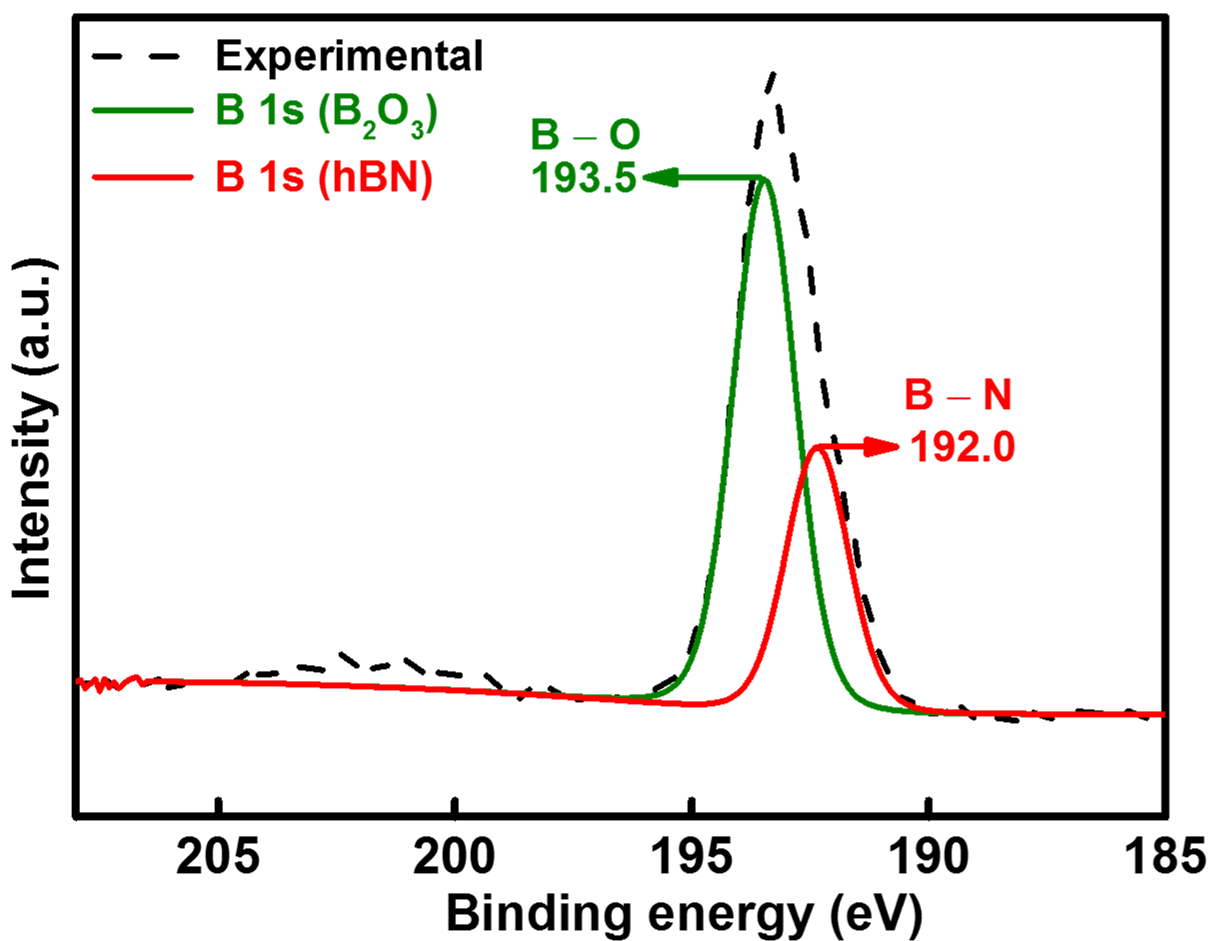
\includegraphics[width=\textwidth]{Figures/BOhBN/oldxps}
\caption{X-ray photoelectron spectra an old hBN cathode.}
\label{Figures/BOhBN:oldxps}
\end{figure}

To conclude that hBN did not play any active role in the old sample cell, boron nitride nano sheets (BNNS) were synthesised and tested as cathodes for AIBs. 
\large{Boron nitride nano sheets (BNNS)}
As mentioned in previous chapters, nano-sized materials increase the contact area between an electrode and electrolyte. They provide short path lengths for both ion diffusion and electron transport, which improves the charge/ discharge rate. The high surface area of the material allows large volume expansion/ contraction associated with ion transport and prevents cathode pulverisation leading to longer cycle-life \cite{zhang_ultrathin_2015,cong_intrinsic_2015}. \\*
\Large{Synthesis of BNNS} \\*
Nano sheets of hexagonal boron nitride were synthesised via mechanical exfoliation. 250 mg of hBN was dispersed in 75 ml isopropanol (IPA) in a 100 ml round bottom flask (RBF). The mixture was heated at 500$^{\circ}$C for 24 hours and was magnetically stirred. To accelerate the dissolution of hBN into IPA, the RBF was then put in an ultrasonic bath for 20 hours. The solution was then left to stand for 2 days and the supernatant was removed in a centrifuge tube. It was centrifuged at a speed of 14000 rpm. The obtained precipitate was washed with acetone to remove residual IPA. The product was dried overnight at 60$^{\circ}$C. 

\begin{figure}[tbh!]
\centering
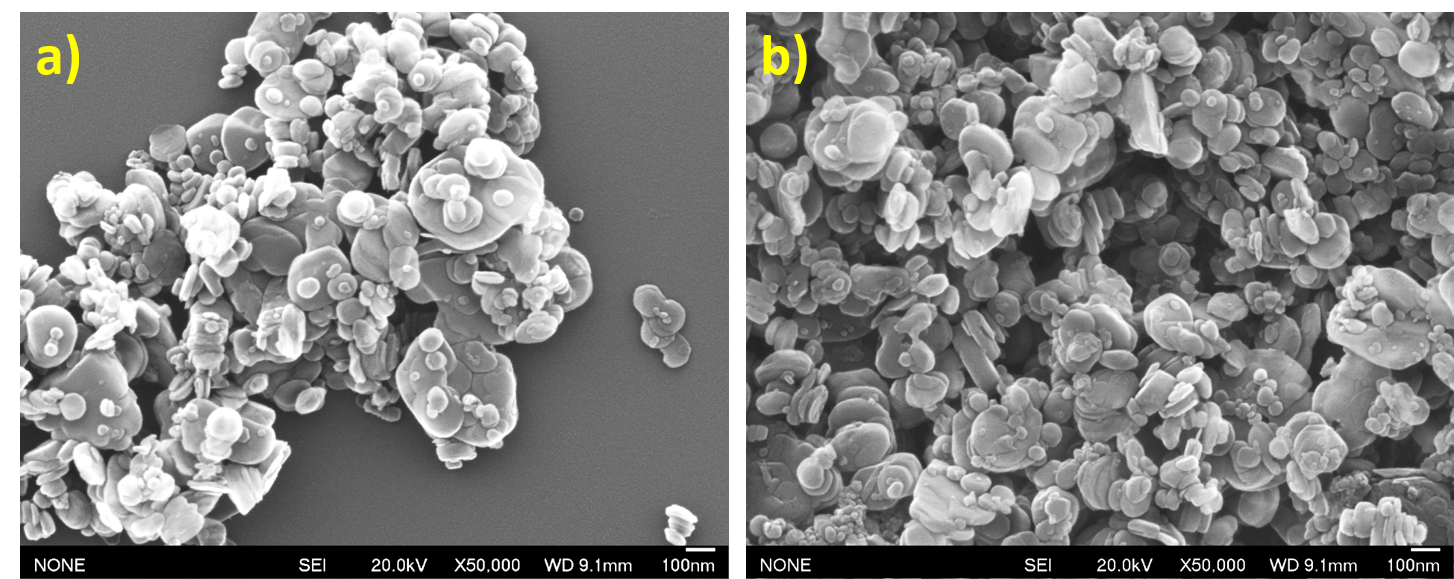
\includegraphics[width=\textwidth]{Figures/BOhBN/BNNSSEM}
\caption{SEM images of hexagonal boron nitride nano sheets.}
\label{Figures/BOhBN:BNNSSEM}
\end{figure}

\begin{figure}[tbh!]
\centering
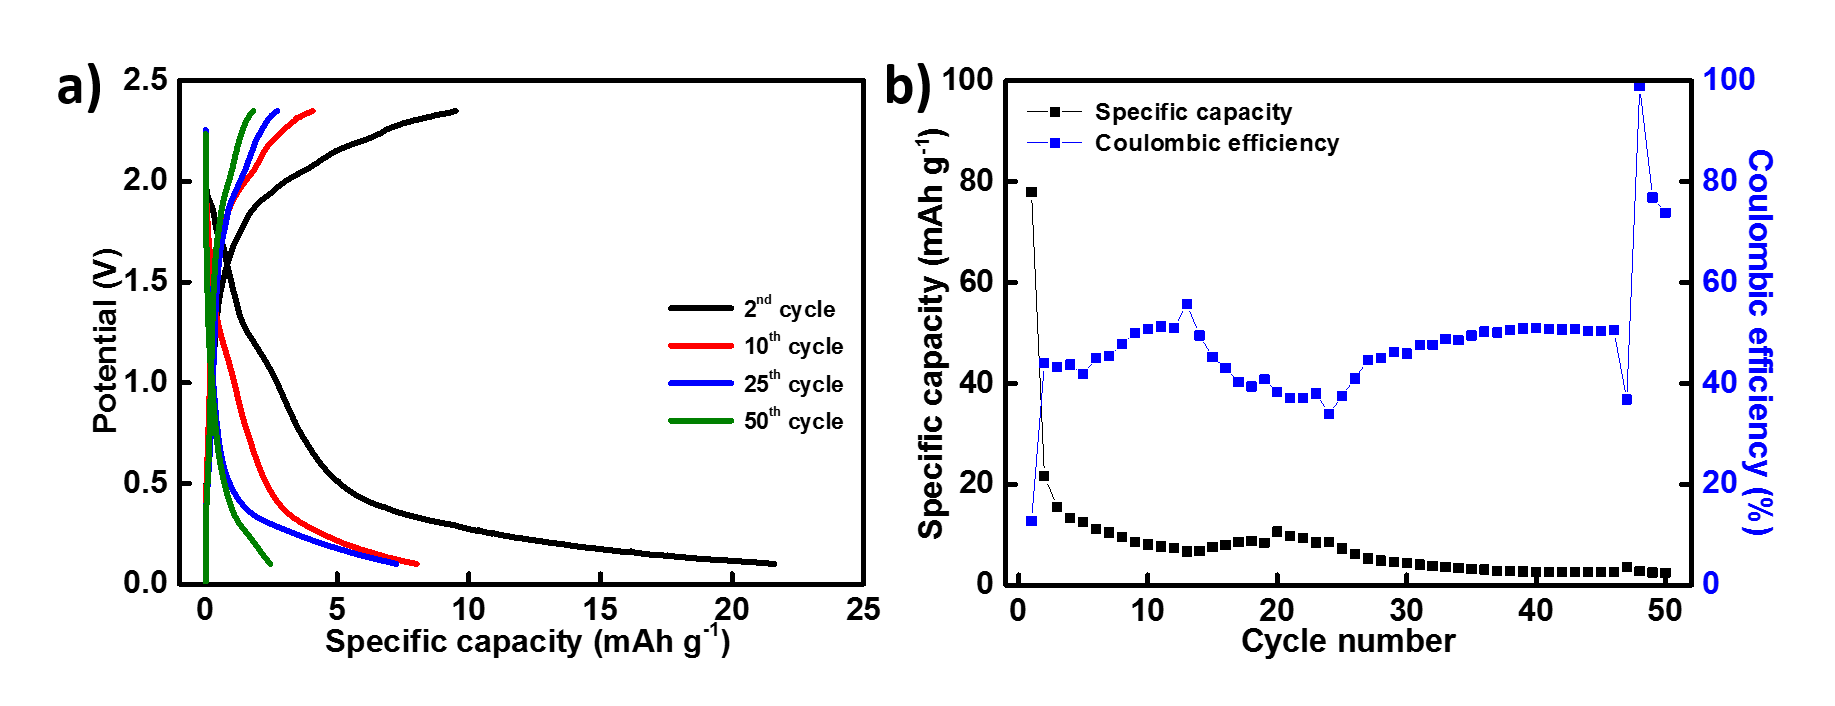
\includegraphics[width=\textwidth]{Figures/BOhBN/BNNSCDCCE}
\caption{Galvanostatic charge/discharge profile of Al/BNNS cell at a current rate of 50 mA g$^{-1}$. The cell achieved 22 mA h g$^{-1}$ in its first cycle, which dropped down to 2 mAh g$^{-1}$ after 50 cycles. Coulombic efficiency was also very low $\sim$50\%. }
\label{Figures/BOhBN:BNNSCDCCE}
\end{figure}

The galvanostatic charge/discharge profile of Al/BNNS is displayed in Figure \ref{Figures/BOhBN:BNNSCDCCE}a and b. Capacity fade and low coulombic efficiencies similar to pure hBN was observed in BNNS as well. This experiment proved that hBN present in the old hBN/\ce{B2O3} mixture, did not have high enough capacity and \ce{B2O3} played a significant role in achieving capacity as high as 270 mAh g$^{-1}$. \\*

\begin{figure}[tbh!]
\centering
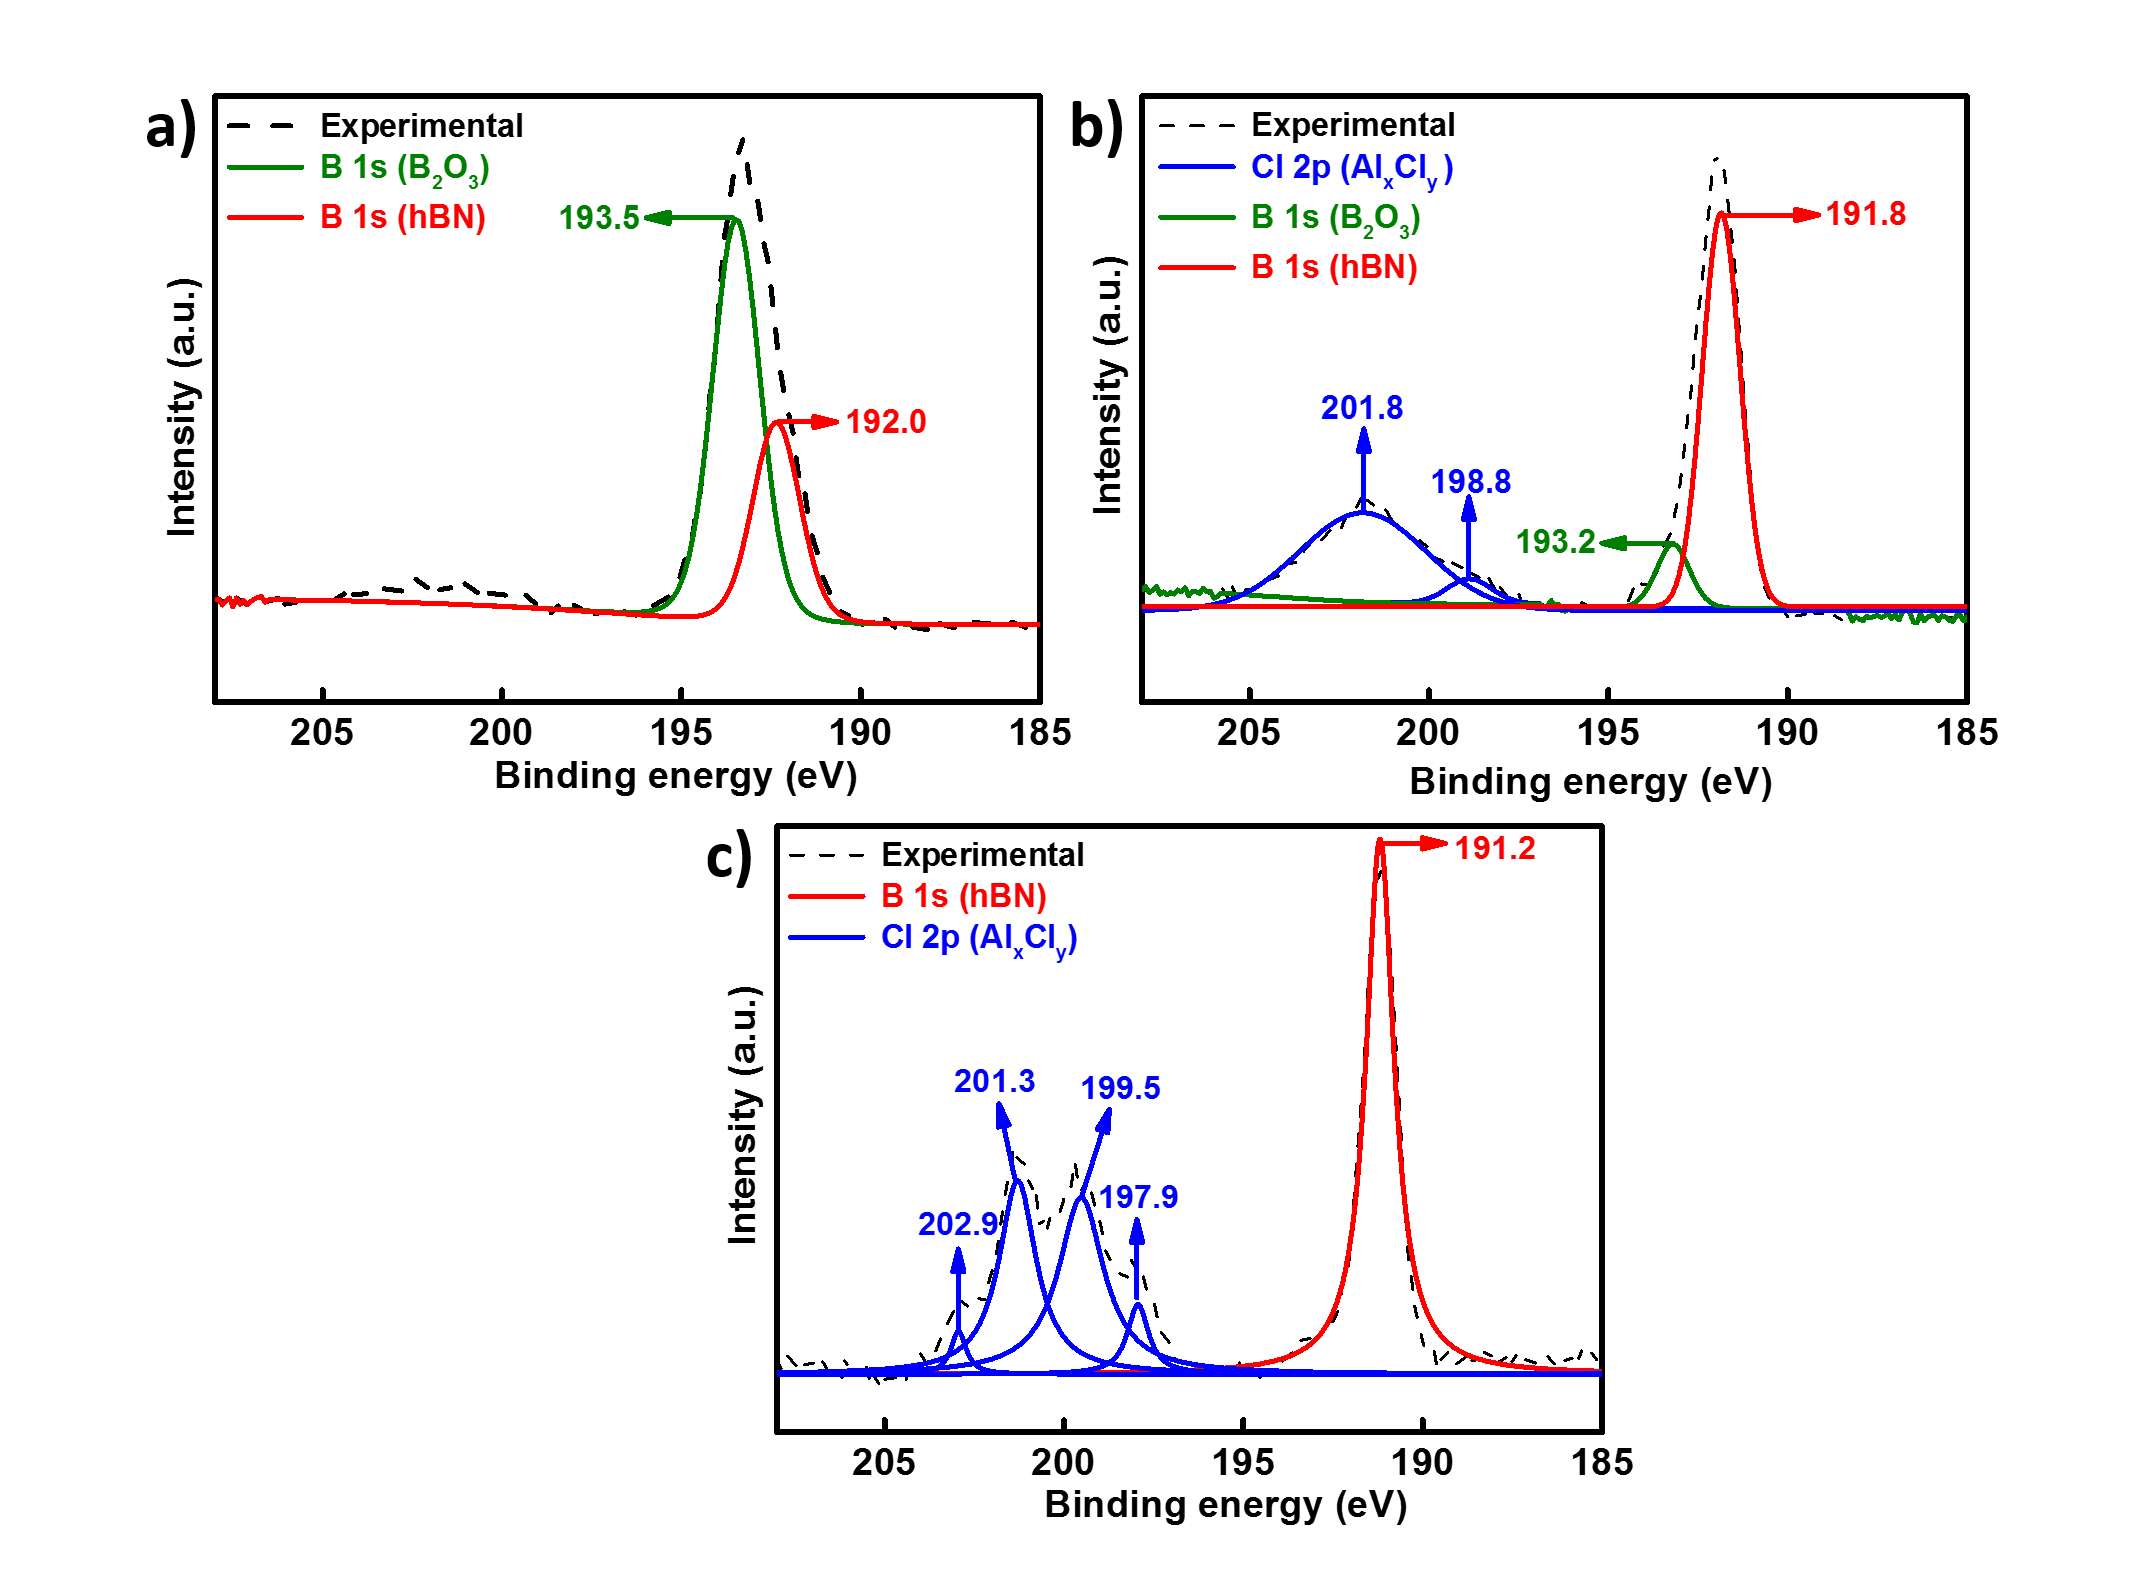
\includegraphics[width=\textwidth]{Figures/BOhBN/oldhBNXPS}
\caption{XPS spectra of a a) pristine, b) charged and c) discharges old hBN cathodes after 30 cycles.}
\label{Figures/BOhBN:oldhBNXPS}
\end{figure}

To examine the changes taking place in the old hBN cathode during charge/discharge cycles, \textit{ex-situ} X-ray photoelectron spectroscopy (XPS) was carried out. The high resolution spectra displaying the binding energies of B 1s and Cl 2p orbitals is shown in Figure \ref{Figures/BOhBN:oldhBNXPS}a-c). The spectra reveal the presence of B and Cl elements for a pristine (Figure \ref{Figures/BOhBN:oldhBNXPS}a) charged (Figure \ref{Figures/BOhBN:oldhBNXPS}b) and discharged (Figure \ref{Figures/BOhBN:oldhBNXPS}c) cathode. Since the pristine electrode was not in contact with the electrolyte, Cl 2p binding energy was absent and the spectra displayed binding energies for boron only. The presence of Cl in the charged and discharged cathodes was mainly derived from the expected intercalation of chloroaluminates into the hBN layers. It can been seen from Figure \ref{Figures/BOhBN:oldhBNXPS}a-c) that the binding energy of B 1s includes a pair of peaks at 193.5 and 192.0 eV before test, which are attributed to B-O (from \ce{B2O3}) and B-N bonds (from hBN) respectively. After charging to 2.35 V, the peak area of the B-O bond significantly decreases. B-N bond from hBN becomes much more dominant. Interestingly, after discharging to 0.3 V, the B-O bond completely disappears as shown in Figure \ref{Figures/BOhBN:oldhBNXPS}c. Binding energy at 191.2 eV was attributed to a B-N bond. Curve fitting for Cl 2p orbital in the charged cathode was problematic. Two broad peaks were fitted into the one broad experimental peak. However, the peak was deconvoluted into 4 peaks at 202.9, 201.3, 199.5 and 197.9 eV after complete discharge. The binding energies (charged cathode) at 193.2 and 191.8 eV are again attributed to B-O from \ce{B2O3} and B-N from hBN respectively. After complete discharge, the B-O bond's binding energy is completely eliminated and only B-N bond remains.

\begin{figure}[tbh!]
\centering
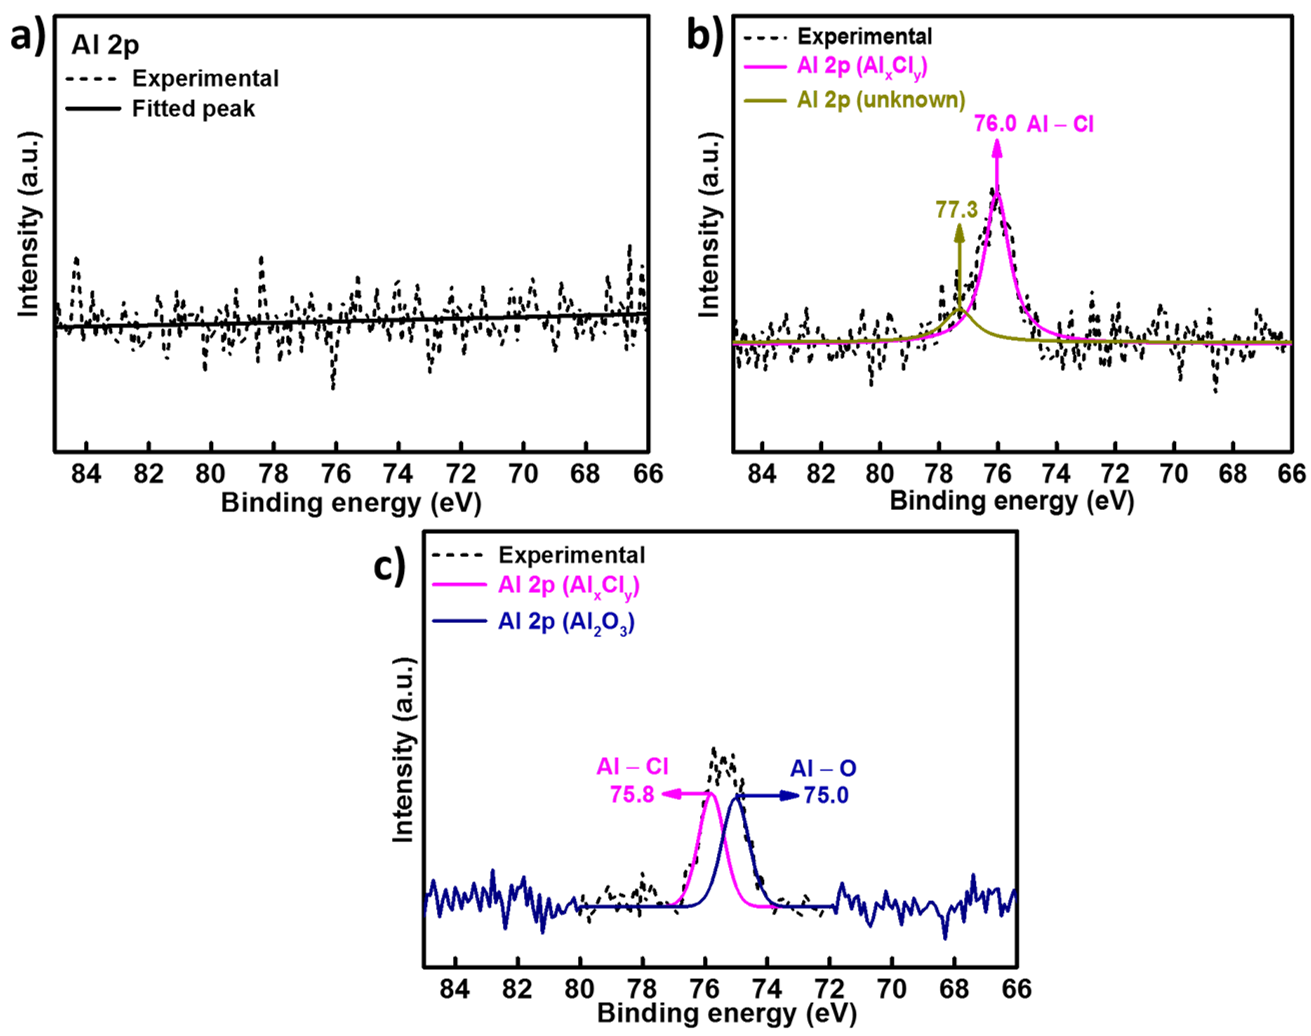
\includegraphics[width=\textwidth]{Figures/BOhBN/hBNAlXPS}
\caption{Honeycomb lattice of a) natural graphite and b) hexagonal boron nitride. Both structures display an interlayer distance of 3.3\AA.}
\label{Figures/BOhBN:hBNAlXPS}
\end{figure}

XPS spectra of Al 2p orbital showed a variation in its binding energies during charge and discharge. During cell charging (Figure \ref{Figures/BOhBN:hBNAlXPS}b), the Al 2p peak deconvolutes into two binding energies at 76.0 and 77.3 eV. The peak at 76.0 eV was attributed to an Al-Cl bond from the chloroaluminates (\ce{AlxCly}). After complete discharge (Figure \ref{Figures/BOhBN:hBNAlXPS}c), the peak shifts to lower binding energies. Experimental curve fitting suggested two binding energies at 75.0 and 75.8 eV. The binding energy at 75.0 eV was attributed to an Al-O bond. It was noted that the binding energy of Al 2p in the oxidised state is 75 eV, which is very close to a typical Al-O bond in \ce{Al2O3} at 74.5 eV \cite{}. This indicated formation of \ce{Al2O3} during discharge. The binding energy at 75.8 eV corresponds to chloroaluminates. It is known that if the electronegativity of the doping element is higher than Al, the electron density around Al decreases and its binding energy increases. Chlorine has a higher electronegativity than oxygen, therefore the peak at higher binding energy in Figure \ref{Figures/BOhBN:hBNAlXPS}c is attributed to \ce{AlxCly} and the lower energy corresponds to \ce{Al2O3}. Since the pristine cathode dis not come in contact with the electrolyte, no peak was observed in Figure \ref{Figures/BOhBN:hBNAlXPS}a for Al. \\*

\begin{figure}[tbh!]
\centering
\includegraphics[width=\textwidth]{Figures/BOhBN/hBNOXPS}
\caption{Honeycomb lattice of a) natural graphite and b) hexagonal boron nitride. Both structures display an interlayer distance of 3.3\AA.}
\label{Figures/BOhBN:hBNOXPS}
\end{figure}

Figure \ref{Figures/BOhBN:hBNOXPS}a-c shows the high resolution O 1s spectra of the pristine (Figure \ref{Figures/BOhBN:hBNOXPS}a), charged (Figure \ref{Figures/BOhBN:hBNOXPS}b) and discharged (Figure \ref{Figures/BOhBN:hBNOXPS}c) cathodes made from the old hBN sample. The O 1s core level spectrum for pristine hBN (Figure \ref{Figures/BOhBN:hBNOXPS}a) was split into two peaks that corresponded to an O-H bond at 535.3 eV. This binding energy was attributed to adsorbed moisture (\ce{H2O}) from the environment. The peak at 534.1 eV was attributed to an O-B bond, which confirmed the presence of \ce{B2O3} in the old hBN sample. In the charged cathode, the major contribution of oxygen comes from \ce{B2O3} at 533.6 eV and the remaining from an O-Al bond with a peak at 531.7 eV, suggesting presence of \ce{Al2O3}.  Figure \ref{Figures/BOhBN:hBNOXPS}c shows the spectrum after complete discharge. The peak obtained was deconvoluted into three binding energies at 535.3, 532.9 and 531.6 eV, corresponding to an O-H bond from adsorbed moisture, O-Al and OH-Al bonds from \ce{Al2O3} and possible formation of \ce{Al(OH)3} respectively \cite{}. Following points were concluded from the XPS analysis:
\begin{itemize}
    \item \ce{B2O3} was present in significant amounts in the old hBN sample. However, it disappears completely after discharge. This might suggest the possibility of a conversion reaction where \ce{B2O3} is being converted into something else during discharge.  
    \item \ce{Al2O3} was formed after complete discharge. AL-Cl bonds were present in both charged and discharged electrodes. Even if deintercalation of ions took place during discharge, not all ions came out and a few \ce{AlCl4^-} ions remained in between the layers. However, an Al-Cl bond might also be a result of electrolyte residue on the cathode. 
\end{itemize}

It was assumed that \ce{B2O3} oxidised the \ce{AlCl4^-} ions to \ce{Al2O3} and itself reduced to elemental boron. However, during charge, elemental B was oxidised to \ce{B2O3} and \ce{Al2O3} was reduced back to \ce{AlCl4^-} ions. The conversion reaction in the form of an equation is mentioned below: 

\begin{equation}
    0.5\ce{B2O3 + AlCl3 + 3e-} \longrightarrow \ce{B + 0.5Al2O3 + 3Cl-}
\end{equation}

\begin{figure}[tbh!]
\centering
\includegraphics[width=\textwidth]{Figures/BOhBN/hBNXPS}
\caption{A wide scan spectrum of pristine (in black), discharged (in red) and charged (in green) hBN (old) cathode. Figure shows the survey spectra with peaks corresponding to aluminum and chlorine observed in the charged and discharged cathodes. Intensity of Al 2p and Cl 2p is higher in discharged cathode.}
\label{Figures/BOhBN:hBNXPS}
\end{figure}

It was important to find out if hBN played any role in this conversion reaction. hBN has a long-range order in its crystal lattice, while \ce{B2O3} has an amorphous structure. An XRD analysis of the old hBN sample would reveal if the layered structure of hBN allows any intercalation of chloroaluminates and undergoes structural changes during cycles. \\*


\begin{figure}[tbh!]
\centering
\includegraphics[width=\textwidth]{Figures/BOhBN/hBNXRD2}
\caption{.}
\label{Figures/BOhBN:hBNXRD2}
\end{figure}

In Figure \ref{Figures/BOhBN:hBNXRD2}, X-ray diffraction patterns of pristine (in black), charged (in green) and discharged (in red) cathodes of old hBN is shown. The patterns are in good agreement with the standard ICDD pattern (04-003-6253) and show the existence of hBN with P6/mmc space group. The miller indices (hkl) of all the characteristic peaks are marked as per the standard pattern. Peak at 2$\theta$ value of 26.5$^{\circ}$ confirms the d-spacing of 3.3\AA\, which matches well with the 002 plane of hBN. An additional shoulder that begins at 22$^{\circ}$ suggested presence of amorphous \ce{B2O3}. Interestingly, a new peak was observed at a 2$\theta$ value of 52.36$^{\circ}$. This peak matched with xxx plane of \ce{B2O3} (ICDD:). There was a slight shift observed for some peaks during the charge and discharge process. The peaks at 100 and 101 shift to lower 2$\theta$ values. This indicated an increase in the d-spacing value. The spacing increased from to 2.17 \AA to 2.22\AA for 100 and from 2.06\AA to 2.16\AA for 101 plane after cycles. In an ideal case, when ions intercalate during charging, the d-spacing increases and then when the ions deintercalate during discharging, the d-spacing returns back to its original value \cite{wang_advanced_2017}. In this case however, the d-spacing does not shift back to its original value after discharge. This suggests that the structural changes that take place during cycles in the hBN crystal lattice are permanent in nature. Since hBN is more crystalline in nature and therefore dominates the XRD data, it was difficult to study the patterns obtained from \ce{B2O3}.  \\*

\textit{Ex-situ} SEM experiments were also conducted to determine the structural changes taking place in the old hBN cathode. Figure \ref{Figures/BOhBN:hBNSEM} displays the SEM images of hBN cathode before and after cycles. Although a few sites showed agglomeration after cycles in Figure \ref{Figures/BOhBN:hBNSEM}b and d, it was difficult to make conclusions from these images.

\begin{figure}[tbh!]
\centering
\includegraphics[width=\textwidth]{Figures/BOhBN/hBNSEM}
\caption{SEM images of a), c) pristine hBN. The hexagonal shape of boron nitride is distinctly visible. Figure\ref{Figures/BOhBN:hBNSEM} b and d) suggest that after a few cycles, the particles agglomerate. The particles retain their distinct hexagonal shape.}
\label{Figures/BOhBN:hBNSEM}
\end{figure}



\section*{Pure boric anhydride \ce{B2O3} as an active material}
To find determine how \ce{B2O3} performed as a cathode material in absence of hBN, cells were assembled using \ce{B2O3} as the active material and the results are shown in Figure \ref{Figures/BOhBN:BOCDC}. 

\begin{figure}[tbh!]
\centering
\includegraphics[width=\textwidth]{Figures/BOhBN/BOCDC}
\caption{Charge/discharge profile of pure \ce{B2O3} as the active material in an AIB at the current rate of 50 mA g$^{-1}$. After 15 cycles, the capacity drops by $\sim$50\%. Coulombic efficiency of Al/\ce{B2O3} is low and  stabilises at $\sim$78\%.}
\label{Figures/BOhBN:BOCDC}
\end{figure}

\ce{B2O3} achieved a discharge capacity of 390 mAh g$^{-1}$ in its first cycle, which decreased to 200 mAh g$^{-1}$ in its second cycle and further dropped down to 90 mAh g$^{-1}$ after 15 cycles. Significant amount of capacity fading was observed, although coulombic efficiency of $\sim$ 78\% was maintained. It was possible that hBN provided structural support to \ce{B2O3}, therefore a combination of both was required to store high amounts of charge Figure \ref{Figures/appendix:hBNrepeat}. 

\begin{figure}[tbh!]
\centering
\includegraphics[width=\textwidth]{Figures/BOhBN/BonhBN}
\caption{Schematic showing the layered structure of hBN supporting \ce{B2O3}. During discharge \ce{AlCl3} reacts with \ce{B2O3} resulting in formation of elemental boron and \ce{Al2O3} and free \ce{Cl-} ions. Further analysis is needed to fully understand the role of hBN.}
\label{Figures/BOhBN:BohBN}
\end{figure}

The ratio of hBN  and \ce{B2O3} in the old sample was unknown. For this reason, different weight ratios of hBN and \ce{B2O3} were investigated as cathodes. The ratios and their performance is tabulated below in Table \ref{tabdiffpc}. All cells achieved discharge voltage plateaus at $\sim$ 0.6 V. 50\% hBN/50\%\ce{B2O3} was the best performing cathode amongst all tested ratios. The results for 1:1 hBN/\ce{B2O3} are displayed in Figure \ref{Figures/BOhBN:hBNBO5050}. Since a conversion reaction (Equation 6.1) was taking place during electron transfer, evaluating a combination of other nitrides and oxides was an important part of this chapter. As the optimum ratio obtained for hBN /\ce{B2O3} cathode was 1:1, all new nitrides and oxides were mixed in that same ratio. 

\begin{table}[tbh!]
\centering
\caption{Comparing performance of hBN/\ce{B2O3} cathodes at different weight percentages.} \label{tabdiffpc}
\begin{tabular}{|ccc|}
\hline
\textbf{Weight \% of} & \textbf{Weight \% of} & \textbf{Discharge capacity in 20th cycle} \\
\textbf{hBN} & \textbf{\ce{B2O3}} & \textbf{mAh g$^{-1}$} \\
\hline
\hline
50 & 50 & 120\\
25 & 75 & 22\\
20 & 80 & 48\\
15 & 85 & 48\\
10 & 90 & 68\\
5 & 95 & 171\\
0 & 100 & 104\\
\hline 
\end{tabular}
\end{table}

\begin{figure}[tbh!]
\centering
\includegraphics[width=\textwidth]{Figures/BOhBN/hBNBOdifpc}
\caption{Charge/discharge curves of aluminium-ion cells with \ce{B2O3}/hBN as cathode in their 20$^{th}$ cycle. The weight percentage varied from 75\%\ce{B2O3}-25\%hBN to 100\% pure\ce{B2O3}.}
\label{Figures/BOhBN:hBNdifpc}
\end{figure}



\begin{figure}[tbh!]
\centering
\includegraphics[width=\textwidth]{Figures/BOhBN/hBNBO5050}
\caption{Charge/discharge curves of hBN/ \ce{B2O3} cells a) for the first 20 cycles at a current rate of 50 mA g$^{-1}$, b) coulombic efficiencies and c) long term cell performance at various current densities ranging from 50 mA g$^{-1}$ to 1500 mA g$^{-1}$ .}
\label{Figures/BOhBN:hBNBO5050}
\end{figure}

Other nitrides such as graphitic carbon nitride g-\ce{C3N4}, aluminium nitride (AlN) and silicon nitride (\ce{Si3N4}) were mixed with \ce{B2O3} in a ratio of 1:1 and tested as cathodes. The results are displayed in Figure \ref{Figures/BOhBN:Bonit}. 
\begin{figure}[tbh!]
\centering
\includegraphics[width=\textwidth]{Figures/BOhBN/Bonit}
\caption{Galvanostatic charge/discharge cycles of cells at different current rates using \ce{B2O3} mixed with other nitrides such as a) \ce{C3N4}, c) AlN and e) \ce{Si3N4} as cathodes. Coulombic efficiencies of b) \ce{B2O3}/\ce{C3N4}, d) \ce{B2O3}/AlN and f) \ce{B2O3}/\ce{Si3N4} cells .}
\label{Figures/BOhBN:Bonit}
\end{figure}

Other oxides such as manganese dioxide (\ce{MnO2}) and titanium dioxide (\ce{TiO2}) were mixed with hBN in a ratio of 1:1 and tested as cathodes for AIBs. The results are displayed in Figure \ref{Figures/BOhBN:BNdifO}.

\begin{figure}[tbh!]
\centering
\includegraphics[width=\textwidth]{Figures/BOhBN/BNdifO}
\caption{Galvanostatic charge/discharge profile and cell efficiencies of AIBs composed of a-b) \ce{hBN}/\ce{MnO2} and c-d) \ce{TiO2}/hBN cathodes.}
\label{Figures/BOhBN:BNdifO}
\end{figure}

A few other combinations were tested as cathodes and the results are displayed in Figure \ref{Figures/BOhBN:othON}.

\begin{figure}[tbh!]
\centering
\includegraphics[width=\textwidth]{Figures/BOhBN/othON}
\caption{Galvanostatic charge/discharge profile and cell efficiencies of AIBs composed of a-b) \ce{MnO2}/\ce{C3N4} c-d) \ce{TiO2}/\ce{C3N4} and e-f) \ce{MnO2}/\ce{Si3N4} cells.}
\label{Figures/BOhBN:othON}
\end{figure}

The research findings from this chapter raises a lot of questions that need to be answered.
\begin{itemize}
    \item {\Large{Role of hBN.}} Is it only providing structural support to \ce{B2O3} or is it actually participating actively in the electron transfer process? If this is just a conversion reaction and hBN is not playing any significant role, why do other nitrides when combined with \ce{B2O3}, do not produce high discharge capacity $\sim$ 250 mAh g$^{-1}$?
    \item {\large{First principle studies of hBN/\ce{B2O3}.}} A conversion-type reaction has been hypothesised for this new material. However, it is important to study the changes taking places inside the cell \textit{in-situ} to fully determine the cell's mechanism. 
    \item {\Large{Using other nitrides and oxides.}} Once the role of nitrides and oxides in this mixture is established, can cheaper alternatives be used instead of hBN? On that note, why do the results in Table \ref{tabdiffpc} differ so much?
\end{itemize}


%% Chapter 6

\chapter{Aluminium-ion batteries using oxides and other materials as cathodes} % Main chapter title

\label{Chapter6} % For referencing the chapter elsewhere, use \ref{Chapter1} 

%----------------------------------------------------------------------------------------

% Define some commands to keep the formatting separated from the content 
\newcommand{\keyword}[1]{\textbf{#1}}
\newcommand{\tabhead}[1]{\textbf{#1}}
\newcommand{\code}[1]{\texttt{#1}}
\newcommand{\file}[1]{\texttt{\bfseries#1}}
\newcommand{\option}[1]{\texttt{\itshape#1}}

%----------------------------------------------------------------------------------------
\section{Theory and background}
\subsection*{Tin oxide, \ce{SnO2}}
Tin (IV) oxide is an inorganic compound with the formula \ce{SnO2}. It finds abundant use as a colorant, polishing powder, for glass coatings and as a sensor for combustible gases. It is a colourless, diamagnetic, amphoteric (reacts with both acid and base) solid. Due to its high theoretical capacity ($\approx$ 782mAh g$^{-1}$), safe handling and environmental-friendliness, \ce{SnO2} is a good cathode candidate for AIBs. Miyasak \textit{et al.} used tin-based amorphous composite oxide (TCO) contains Sn(II)-O as the active center for lithium-insertion and other glass-forming elements, which made an oxide network \cite{idota_tin-based_1997}. In its charged state, TCO accepted 8 moles of lithium ions per unit mole. However, it underwent large volumetric changes $\approx$ 300{\%}, which caused slow diffusion kinetics. It further resulted in agglomeration and pulverisation of cathodes after continuous charge-discharge cycles. This resulted in capacity fading. To improve the battery performance, carbon-based materials were added to \ce{SnO2}. It not only provided a high surface area that would act as a buffer for volume expansion/shrinkage, but also would improve the conductivity of the active material. Based on this concept, Nowak \textit{et al.} \cite{nowak_composites_2018}
Carbon is known not to react with tin and does not form tin carbide \cite{}. It is very crucial in terms of utilizing carbon as a buffer in preventing electric contact loss of the tin negative electrode with the current collector\cite{}. The historical background for modification of tin oxides with carbonaceous material origins from Lee \textit{et al.} who obtained synthetic graphite modified by a highly dispersed tin oxide which improved the cell's performance \cite{navarro-suarez_2d_nodate}. 
It was observed that carbon coating on \ce{SnO2} surface prevents their agglomeration and volume expansion. A smaller particle size (like nanorods\cite{}, nanosheets\cite{}, nanospheres\cite{}, nanowires\cite{}, nanotubes\cite{}, nanoflowers\cite{}) or/and a porous structure of the active material would further alleviate the contact area between the electrode and the electrolyte, accelerating the transport of ions. 
We tested SnO2 and Sb-SnO2 as cathodes for AIBs. Antimony is commonly used as a n-type dopant which increases the conductivity of SnO2 by increasing its band gap. 
\subsection*{Molybdenum trioxide, \ce{MoO3}}

%Boron nitride is a thermally and chemically resistant compound. It exists in various crystalline forms that are isoelectronic to a similarly structured carbon lattice and therefore is also called 'inorganic graphite'. The hexagonal form corresponding to graphite is the most stable and soft among BN polymorphs, and is therefore used as a lubricant and an additive to cosmetic products. The most stable crystalline form is the hexagonal one, also called hBN, $\alpha$BN, and graphitic boron nitride. Hexagonal boron nitride has a layered structure similar to graphite. Within each layer, boron and nitrogen atoms are bound by strong covalent bonds, whereas the layers are held together by weak van der Waals forces. While graphite has non-polar homonuclear C−C intralayer bonds, h-BN presents highly polar B−N bonds resulting in different optimal stacking modes of the two materials in the bulk form. Furthermore, the static polarizabilities of the constituent atoms considerably differ from each other, suggesting large differences in the dispersive component of the interlayer bonding. Despite these major differences, both materials present practically identical interlayer distances\cite{}. 
\subsection*{graphitic Carbon Nitride, g-\ce{C3N4}}
\subsection*{Prussian blue, \ce{C19Fe7N18}}
\section{Experimental methods}
Same as discussed in Chapter\ref{chap3}.
\section{Results and discussions}
\section{Conclusion and future work}
%% Chapter 7
\section*{Preface}
To find cheaper alternatives to the state-of-the-art, a wide range of solvents and current collectors were investigated while preparing cathodes and their performance was recorded.   
\newpage

\chapter{Impact of solvents and current collectors on rechargeable AIBs} % Main chapter title
\label{chap7} % For referencing the chapter elsewhere, use \ref{Chapter1} 

\section{Introduction}

Battery electrodes are manufactured by casting a slurry onto a current collector. The slurry contains an active material, conductive carbon, and a polymer binder dispersed in a solvent. Synergy between the different components in a slurry enhances the electrochemical property of the electrode by placing the electrode particles closer together and increasing the conductivity of the slurry \cite{zheng_cooperation_2012}.
However, the role of one additive is controlled by the other. For example, a more non-conductive binder and an oxide active material, would inhibit the electronic conductivity resulting from carbon additives, and nano-sized carbon additives can spoil the binding effect between particles of the active material \cite{guy_novel_2006, seki_effect_2004}. Therefore, optimization of electrode compositions is essential for fabrication of high-quality electrodes. Furthermore, a good solvent should provide:
\begin{itemize}
    \item high viscosity,
    \item high stability,
    \item high dispersity,
    \item avoid decomposition of electrolyte and 
    \item improve the compatibility of cathode slurry and electrolyte.
\end{itemize}
A non-uniform coating on the current collector, results in an uneven weight distribution \cite{ludwig_solvent-free_2016}. The solvent should prevent agglomeration of the particulate materials as that would lead to a poorly flowing slurry. This deteriorates the battery performance and leads to a slower transfer of energy to or from the cell. N-methyl pyrrolidinone (NMP) is chosen as the solvent because it is still the premium choice for cathodes in commercial lithium ion cells. It is polar and its functional groups provide enhanced adhesion with binders, especially polyvinylidene fluoride (PVDF) (Figure \ref{Figures/chap7fig:NMP}). After a slurry has been mixed uniformly, it is cast onto a metal foil and dried. Solvent evaporation is necessary for cell fabrication. Since NMP is an expensive solvent and an environment pollutant, ideally an NMP recovery system must be in place during the drying process to recover evaporated NMP. However, new coating techniques and different solvents are now being developed to make battery manufacturing more economical. \cite{liu_effective_2014-1,spreafico_pvdf_2014-1, liu_effects_2008-1, lee_effect_2010-1, wenzel_challenges_2015, lee_selection_2017, stein_non-aqueous_2016}. In LIBs, the NMP/PVDF couple was replaced by water/elastomers (styrene-butadiene rubber), however the anode was not compatible with water and the batteries failed to deliver desired energy densities \cite{lee_novel_2007, li_effects_2005}. 
To find a cheaper alternative to NMP, we investigated a few solvents such as isopropyl alcohol (IPA), toluene, acetone, methanol, butanol, dimethylsulfoxide (DMSO), dimethylformamide (DMF), dimethylacetamide (DMA), and acetonitrile (listed in Table \ref{tab1}) and used them for preparing cathode slurries . 

\begin{figure}[tbh!]
\centering
\includegraphics[width=0.75\textwidth]{Figures/chap7fig/NMP}
\caption{Structure of N-methyl pyrrolidinone, NMP.}
\label{Figures/chap7fig:NMP}
\end{figure}

\begin{table}
\caption{List of solvents used for making cathode slurries.} \label{tab1}
\begin{center}
 \begin{tabular}{|c|c|c|c|} 
 \hline
 \textbf{Solvent} & \textbf{Polarity} & \textbf{Boiling point} & \textbf{Price}\\
 \textbf{} & \textbf{} & \textbf{($^{\circ}$C)} & \textbf{(\$L$^{-1}$)}\\
 \hline
 \hline
IPA & 0.55 & 82 & 83 \\
Toluene & 0.09 & 110 & 88 \\
Acetone & 0.35 & 56 & 93 \\
Methanol & 0.76 & 65 & 112 \\ 
Butanol & 0.59 & 117 & 143 \\
DMSO & 0.44 & 189 & 198 \\
DMF & 0.39 & 153 & 207 \\
DMA & 0.35 & 165 & 211 \\
Acetonitrile & 0.35 & 82 & 221 \\
NMP & 0.35 & 202 & 259 \\
 \hline
\end{tabular}
\end{center}
\end{table}

\section{Experimental methods}
NMP/PVDF mixtures were made by dissolving 18 mg of PVDF in 1.25 ml of anhydrous NMP. A given amount of SPCB and active material was dispersed in the PVDF/NMP solution to meet the desired active material:SPCB::PVDF ratios. To ensure the thorough mixing of the SPCB particles into the polymer solution, the solution was stirred overnight. Electrode laminates were prepared by casting the slurries onto a metal foil by the doctor blade method. All the electrode films had approximately the same loading of active material (around 5-6 mg cm$^{-2}$) to eliminate the thickness effect on the electrochemical performance of the electrode. After coating the foils, the laminates were dried at 80$^{\circ}$C for two hours and then at 120$^{\circ}$C for 12 hours under vacuum. It is essential that the solvent completely evaporates and is removed from the coated electrode. It was noted that DMSO/PVDF, DMF/PVDF, DMA/PVDF and NMP/PVDF mixtures resulted in clear solutions, while ethanol, isopropanol, toluene, acetone, methanol and butanol had a cloudy appearance. 
In addition, the boiling point of the solvents was a limiting factor. High volatility of the solvents resulted in quick drying of the slurries. Cathodes that used low boiling points such as acetone, ethanol, methanol isopropanol and acetonitrile, developed cracks on their surface due to high evaporation rates, which rapid drying of the coating before they were vacuum dried.
Slurries that used DMSO, DMF, DMA, NMP, butanol and toluene as solvents yielded crack-free coatings. Consequently, the cathodes that were used for electrochemical tests were the ones made from DMSO, DMF and DMA.
The cathodes were tested via galvanostatic charge/discharge cycles in Figure \ref{Figures/chap7fig:hBNsolvents}. Same active material was used for all the cells, which is why the discharge capacities did not vary a lot. Figure \ref{Figures/chap7fig:hBNsolvents}b  shows that overall capacity of DMA based cathode was highest in its first cycle. However, it also recorded the fastest capacity fading. A possible explanation could be deducted from the coulombic efficiencies shown in Figure \ref{Figures/chap7fig:hBNsolventsCE}b. With efficiencies higher than 100\% for almost every cycle, it is likely that a few side reactions took place. DMSO-based cathodes showed consistent but high cell efficiencies >100\% (Figure \ref{Figures/chap7fig:hBNsolventsCE}a). 

\begin{figure}[tbh!]
\centering
\includegraphics[width=\textwidth]{Figures/chap7fig/hBNsolvents}
\caption{Galvanostatic charge and discharge curves of aluminium-ion cells using different solvents, a) DMSO, b) DMA, c) DMF and d) NMP.}
\label{Figures/chap7fig:hBNsolvents}
\end{figure}

\begin{figure}[tbh!]
\centering
\includegraphics[width=\textwidth]{Figures/chap7fig/hBNsolventsCE}
\caption{Performance of aluminium-ion cells using different solvents, a) DMSO, b) DMA, c) DMF and d) NMP.}
\label{Figures/chap7fig:hBNsolventsCE}
\end{figure}

Figure \ref{Figures/chap7fig:hBNsolvents}c showed that with increasing cycle numbers, capacity of DMF-based cathode decreased faster than NMP based cathode, Figure \ref{Figures/chap7fig:hBNsolvents}d. Though, cell efficiency for DMF (98\%), Figure \ref{Figures/chap7fig:hBNsolventsCE}c, was better than that for NMP-based cathode (>100\%), Figure \ref{Figures/chap7fig:hBNsolventsCE}d.

\begin{figure}[h!]
\centering
\includegraphics[width=\textwidth]{Figures/chap7fig/hBNsolventSEM}
\caption{Scanning electron microscopic images of pristine cathodes using a) DMSO, b) DMA, c) DMF and d) NMP as solvents.}
\label{Figures/chap7fig:hBNsolventSEM}
\end{figure}

Figure \ref{Figures/chap7fig:hBNsolventSEM} shows the SEM images. With DMSO and DMA, the electrode is shown to be a stack of active material, Figure \ref{Figures/chap7fig:hBNsolventSEM} a and b. SPCB agglomerates are not homogeneously dispersed in the electrode, since these particles easily flocculate as a result of their large surface area. DMF and NMP-based cathodes appeared evenly distributed and seemed to be immersed into a matrix of PVDF and SPCB composite, Figure \ref{Figures/chap7fig:hBNsolvents} c and d.\\
Overall, DMF-based cathodes maintained their specific discharge capacity after 50 cycles, with a very high coulombic efficiency $\sim$ 100\%. It seems DMF can be alternatively used as an electrode solvent, which would reduce the battery production costs. 

\subsection*{Current collectors}

\begin{table}
\caption{List of materials used as current collectors in increasing order of their marker price.} \label{t2}
\begin{center}
 \begin{tabular}{|c|c|c|c|} 
 \hline
 \textbf{Material} & \textbf{Thickness} & \textbf{Price} & \textbf{Conductivity} \\
 \textbf{Material} & \textbf{(mm)} & \textbf{(\$)} & {X 10$^{7}$}({$\Omega$}m)$^{-1}$ \\
  \hline
 \hline
Steel & 0.1 & 1.0 & 0.6 \\ 
Carbon paper & <0.1 & 1.2 & 6.5 \\
Aluminium & 0.1 & 3.04 & 3.6 \\
Brass & 1 & 5.07 & 1.4 \\
Copper & 0.1 & 9.91 & 5.9 \\ 
Nickel foam & 1 & 17.93 & 1.4 \\
Molybdenum & 0.1 & 39.61 & 1.9 \\
\hline
\end{tabular}
\end{center}
\end{table}

A current collector is a conductive solid connected to the electrode with external loading. The primary role of a current collector is to provide support to the electrodes (cathode and/or anode), collect the accumulated electrical energy from the electrode. A common current collector is a metal foil onto which a slurry is coated. A good connection between the active material and the metal foil is established only after a slow drying process which evaporates the solvent and binds it to the CC. Many metal foils have been used as metal/alloys foils in LIBs, such as nickel, copper, aluminium and steel. LIBs use two metal foils. Copper is used for the anode and aluminium is used for the cathode. This is because the two metal foils are stable at different potentials. Copper is electrochemically stable at a lower potential--
 V vs. Li\ce{Li+}, whereas aluminium is stable at a higher potential-1.34 V vs. Li\ce{Li+}. Aluminium cannot be used in our setup because it acts an anode and any contact between the active material and the anode would create a short circuit.  A CC should allow a stable flow of electrons, and should be ionically insulated. A good CC should be mechanically robust, and freestanding (usually with a macroscale size). Since a CC should be electrochemically inert, we could not use nickel foil because it oxidised at 1.1 V vs. Al/\ce{Al3+}. Steel, which is light in weight and cheap, underwent a vigorous reaction with our electrolyte and resulted in undesirable products, which resulted in rapid capacity decay and a very short cycle life. It seemed that \ce{AlCl3}/EmImCl corroded in presence of steel as can be seen in Figure \ref{Figures/chap7fig:steeleffect}. To avoid this, a CC should be within the electrochemical window if the electrolyte being used. Chemical potential of a CC ({$\mu${${_{cc}}$}} < 2.5 V) vs. Al/\ce{Al$^{3+}$}. Molybdenum foil ticked all the boxes and therefore was chosen as the CC in all our battery tests.  
 We compared the cell performances of all cells using different CCs, showed in Figure \ref{Figures/chap7fig:hBNCCCDC}. Firstly, carbon as a CC stands out from the other CCs. The cell recorded the highest discharge capacity at 82 mAh g$^{-1}$ (in green). When run for longer, the capacity was retained at 70 mAh g$^{-1}$ after25 cycles. The curve was exceptionally similar to the CDCs of an Al/graphite cell (inset Figure \ref{Figures/chap7fig:hBNCCCDC}b). This lead us to the conclusion that hBN became dormant in this cell and graphitic nature of the carbon paper took over and acted as the active material intercalating the \ce{AlCl4-} ions during charge. Steel, nickel, copper, brass and copper foils did not allow any charge or discharge to take place. Despite applying a continuous current, the charges seemed to accumulate and provided an unstable flow of electrons. Copper is a highly conductive metal; when aluminium electroplates, a few ions might get deposited on the CC creating a short circuit. Steel on the other hand contains chromium, which reacts with \ce{AlCl3}/EmImCl and some greenish stuff can be observed after we open the cell Figure \ref{Figures/chap7fig:steeleffect} \cite{reed_roles_2013}. This confirms that a side reaction took place, which consumed the electrolyte. Brass is less conductive than copper, as seen in Table \ref{t2}, and it contains other metals which have impeded the cell reaction and its capacity.   
%The battery performance results are shown in figure 6. It can be seen that the charging behaviour of brass, copper and aluminium have a similar tendency. Starting from different voltages, charging the system does not result in an actual increase in voltage, thus charge built-up as desired. As shown in figure 6 a), brass, copper and aluminium tend to reach a specific equilibrium voltage regardless of the energy provided to the system. Energy consumption without any charging indicates other processes being present consuming the provided energy. It is assumed that the energy consumed is used to disintegrate the substrate material. Ideally, the substrate is not in direct contact with the electrolyte. In reality however there will always be some sort of contact area present. The Al atoms in the aluminium and eventually the iron or chromium atoms present in the brass and copper are resulting in the disintegration of the substrates as such. As a reference how a single charging/discharging cycle should appear, figure 6 b)	shows a complete cycle for a BN RAB using a molybdenum substrate. Here the desired charge built-up can be observed until reaching the cut-off limit of 2.4V and the following discharging can be observed. A very unique charging behaviour could be observed for carbon coated aluminium as a substrate for the hBN slurry as shown in figure 6 c). A mixture of fast charging and abrupt rapid discharging can be observed. Knowing the tendency of the aluminium shown in figure 6 a) to completely discharge to the cutoff voltage of 0.1, it can be assumed that the rapid discharging behaviour results from the underlying aluminium. As discussed in section 2, carbon based RAB have been shown to work well and achieve high charging rates. Therefore it is assumed that the charging phases are either caused by the BN cathode material or by the underlying carbon coating. Even though the just discussed tested alternatives did not succeed in charging at all, Ni foam and Carbon paper did successfully charge and discharge. The corresponding capacities are shown in figure 6 d). The fact that the capacity of the battery with Ni foam as substrate is noticeable lower is caused by the fact that nickel oxidises at voltages exceeding 0.9 V. This relatively low cutoff voltage is one reason why the capacity is rather low. It can be noticed that carbon paper as a substrate has a very high capacity. Comparing the achieved result however with results previously achieved by researchers of the VUW using carbon paper only, showed that that the overall performances are very much alike. This leads to the conclusion, that contrary to the desired hBN, mainly the carbon paper participated in the intercalation/deintercalation process. Therefore it is not a suitable substrate candidate for the specific use in the hBN based batteries due to the ions preferred affinity towards the carbon paper rather than to the hBN cathode material.
\begin{figure}[tbh!]
\centering
\includegraphics[width=\textwidth]{Figures/chap7fig/steeleffect}
\caption{SEM images of pristine hBN cathodes using a) DMSO, b) DMA, c) DMF and d) NMP solvents.}
\label{Figures/chap7fig:steeleffect}
\end{figure}
\begin{figure}[tbh!]
\centering
\includegraphics[width=\textwidth]{Figures/chap7fig/hBNCCCDC}
\caption{Galvanostatic cycles using hBN as the active material with a) steel and nickel foils (black), copper sheet (red), brass sheet (blue) and carbon paper (green) as current collectors in a two-electrode setup at a current rate of 40 mA g$^{-1}$. b) Performance of Al/hBN cell using carbon paper as the current collector which showed graphite dominating as active material (inset: CDC curve of an Al/graphite cell) }
\label{Figures/chap7fig:hBNCCCDC}
\end{figure}

\section{Conclusion and future outlook}
Replacing NMP with a cheaper solvent would be beneficial when commercialising AIBs. However, no solvent has proven to be as efficient as NMP yet. LIB plants recycle NMP on a regular basis. During vacuum drying process, NMP is collected from the exhaust gases and is used to clean equipment and is reused. This method can be applied while manufacturing AIBs, which would further reduce the battery production costs. 
Molybdenum, titanium and ITO turned out to be a good current collectors for our AIBs. Although a CC is inactive in a cell, however it occupies enough space- almost 9\%! If this number is reduced, the cell will record a higher energy density. One can use a thinner foil (structurally stable) instead of a thick one to attain a higher capacity value. In fact a thicker coating of the active material might seem as a solution but that limits the ion and electron transport across the electrode leading to a lower cycle life. 3D current collectors based on carbon might be the way to go. In LIBs, graphite foam has been used as a CC, since it does not intercalate at a potential >0.5V. Ruoff \textit{et al.} \cite{ji_ultrathin_2012} use graphene foam as a current collector for the first time. A 3D CC not only provides a dense interconnected structure that can rapidly transport /diffuse ions, but also an excellent conductivity. CC with a large pore volume accommodates expansion of active material would also prevent cathode pulverisation. 

%% Chapter 9
\chapter{Conclusion/ summary} % Main chapter title
\label{chap9} % For referencing the chapter elsewhere, use \ref{Chapter1} 


%	THESIS CONTENT - APPENDICES

\appendix % Cue to tell LaTeX that the following "chapters" are Appendices

% Include the appendices of the thesis as separate files from the Appendices folder
% Uncomment the lines as you write the Appendices

%% Appendix Template
\chapter{Appendix} % Main appendix title
\label{appA} % Change X to a consecutive letter; for referencing this appendix elsewhere, use \ref{AppendixX}

\begin{figure}[tbh!]
\centering
\includegraphics[width=\textwidth]{Figures/appendix/hBNrepeat}
\caption{Galvanostatic charge/discharge curves of an Al/hBN cells using old hBN using a two-electrode setup at a current rate of 40 mA g$^{-1}$. }
\label{Figures/appendix:hBNrepeat}
\end{figure}

\begin{figure}[tbh!]
\centering
\includegraphics[width=\textwidth]{Figures/appendix/pouchCE}
\caption{a) Coulombic efficiency recorded for 1600 cycles of an Al/hBN pouch cell assembled in IKTS, Germany.}
\label{Figures/appendix:pouchCE}
\end{figure}

\begin{figure}[tbh!]
\centering
\includegraphics[width=\textwidth]{Figures/appendix/hBNmultiattempts}
\caption{CDCs of Al/hBN cells using pure hBN, 98\% pure, $\approx$1 $\mu$m in size using similar assembly conditions. All cells were run at a current rate of 40 mA g$^{-1}$. Despite repeated attempts, none of the cells recorded a capacity above 50 mAh g$^{-1}$. This was an issue because we were trying to replicate our previous results where an Al/hBN cells recorded capacities above 100 mAh g$^{-1}$, Figure \ref{Figures/appendix:hBNrepeat}.}
\label{Figures/appendix:hBNmultiattempts}
\end{figure}

\begin{figure}[tbh!]
\centering
\includegraphics[width=\textwidth]{Figures/appendix/pouchcellCDCCE}
\caption{a-c) Cell performance of various Al/hBN pouch cells assembled in ITKS, Germany. None of the cells managed to achieve capacities above 50 mAh g$^{-1}$. d) Coulombic efficiency of an Al/hBN cell run for thousand cycles at a current rate of 40 mA g$^{-1}$. }
\label{Figures/appendix:pouchcellCDCCE}
\end{figure}
\begin{figure}[tbh!]
\centering
\includegraphics[width=\textwidth]{Figures/appendix/WS2CDCCE}
\caption{ a) Galvanostatic charge/discharge cycles, and b) coulombic efficiency of an Al/\ce{WS2} cell for 10 cycles at a current rate of 50 mA g$^{-1}$. A distinct plateau was seen during discharge at 0.68 V and a charging plateau was observed at 1.0 V vs \ce{Al$^{3+}$}/Al. \ce{WS2} has a layered structure similar to \ce{MoS2} with an interlayer distance of 6.18 \AA. Looking at the CDCs, a few \ce{AlCl4-} ions manage to intercalate but it seems the side reactions taking place at the electrode/electrolyte interface prevent the cell from achieving high specific capacities.}
\label{Figures/appendix:WS2CDCCE}
\end{figure}

%----------------------------------------------------------------------------------------
%	BIBLIOGRAPHY
%----------------------------------------------------------------------------------------

\printbibliography[heading=bibintoc]

%----------------------------------------------------------------------------------------

\end{document}  
